\chapter{Correction and validation of the MC simulation}
\label{ref:mc-cor}

This chapter describes updates to form factor modelling and corrections to
detector responses on MC.
The procedure is the following:
%%%%
First, the outdated form factor models are updated with a reweighting
procedure documented in \cref{ref:mc-cor:ff}.
%%%%
Then, the known problematic detector responses,
such as tracking efficiency and \B production kinematics,
are corrected.
This is termed as \emph{initial reweighting}, and is described in
\cref{ref:mc-cor:init}.
%%%%
After, a \emph{preliminary} fit is performed to build
\emph{post-fit cocktail},
with the building procedure outlined in \cref{ref:mc-cor:postfit-cocktail}.
Finally, agreements between data and cocktail on additional kinematic
and geometric variables of the \B decay daughters are assessed,
and a multi-stage reweighting process is
performed to correct disagreements if necessary.
Outlined in \cref{ref:mc-cor:final}, such procedure is called \emph{final
reweighting}.


\section{Form factor models}
\label{ref:mc-cor:ff}

The form factor model for a $B \rightarrow D \ell\neulb$ process \emph{defines}
the truth-level \qSq distribution (with angular variables integrated out) which
in turn affect the estimated \qSq which is a fit variable.
Therefore, it is important to use the state-of-art form factor models.
Naively this is hard, because the form model model is defined at MC generator
level, any change in form factor may require a regeneration of all MC samples.
In reality, however, for a given phase space point\footnote{
    % FIXME: Implement the reference!
    The phase space is parameterized by \qSq and possibly angular variables,
    as defined in \cref{ref:theory:ff}.
}  \PSpt, the probability density that an event is generated \emph{at}
\PSpt is proportional to the differential decay rate evaluated at
\PSpt.
%%%%
For an event (or equivalently a given \PSpt point)
generated with an old form factor model,
its contribution (weight) in the new model is given by the ratio of differential
decay rates
\begin{equation}
    r = \left.
            \frac{d\Gamma_\text{target} / d\PSpt}{d\Gamma_\text{source} / d\PSpt}
        \right|_\text{eval at phase space point}
\end{equation}
So a change in form factor model is equivalently to a reweight, with weight given
by $r$.

\Hammer, the current state-of-art form factor reweighting program, is used
in this analysis to reweight
$B \rightarrow (\Dz| \Dstar| D^{**}) \lepton\neulb$ MC samples.
\Hammer implements a fast reweighting procedure with a multi-dimensional
expansion of form factors around a central point in the form factor parameter
space.
The details of the form factor reweighting are given below.

\subsection{$B \rightarrow \Dz$ decays}

The \Dz MC samples are generated with an up-to-date CLN form factor model.
Still, it is reweighted to a BGL model whose parameters are taken
from Table 4 in \cite{Bigi_2016} at $N = 2$, as these
parameters are obtained from a fit to lattice and experimental data.
The $N = 2$ is chosen because it is the only case where the correlation matrix
is reported.
\Cref{fig:ff-d0} shows the change of true \qSq distributions due to form factor
reweighting for \Dz samples.
The changes are minimal because both models are up-to-date.

% Generated in /rdx-run2-analysis with:
%   make plot-all-ff-rwt
\begin{figure}[htb]
    \centering
    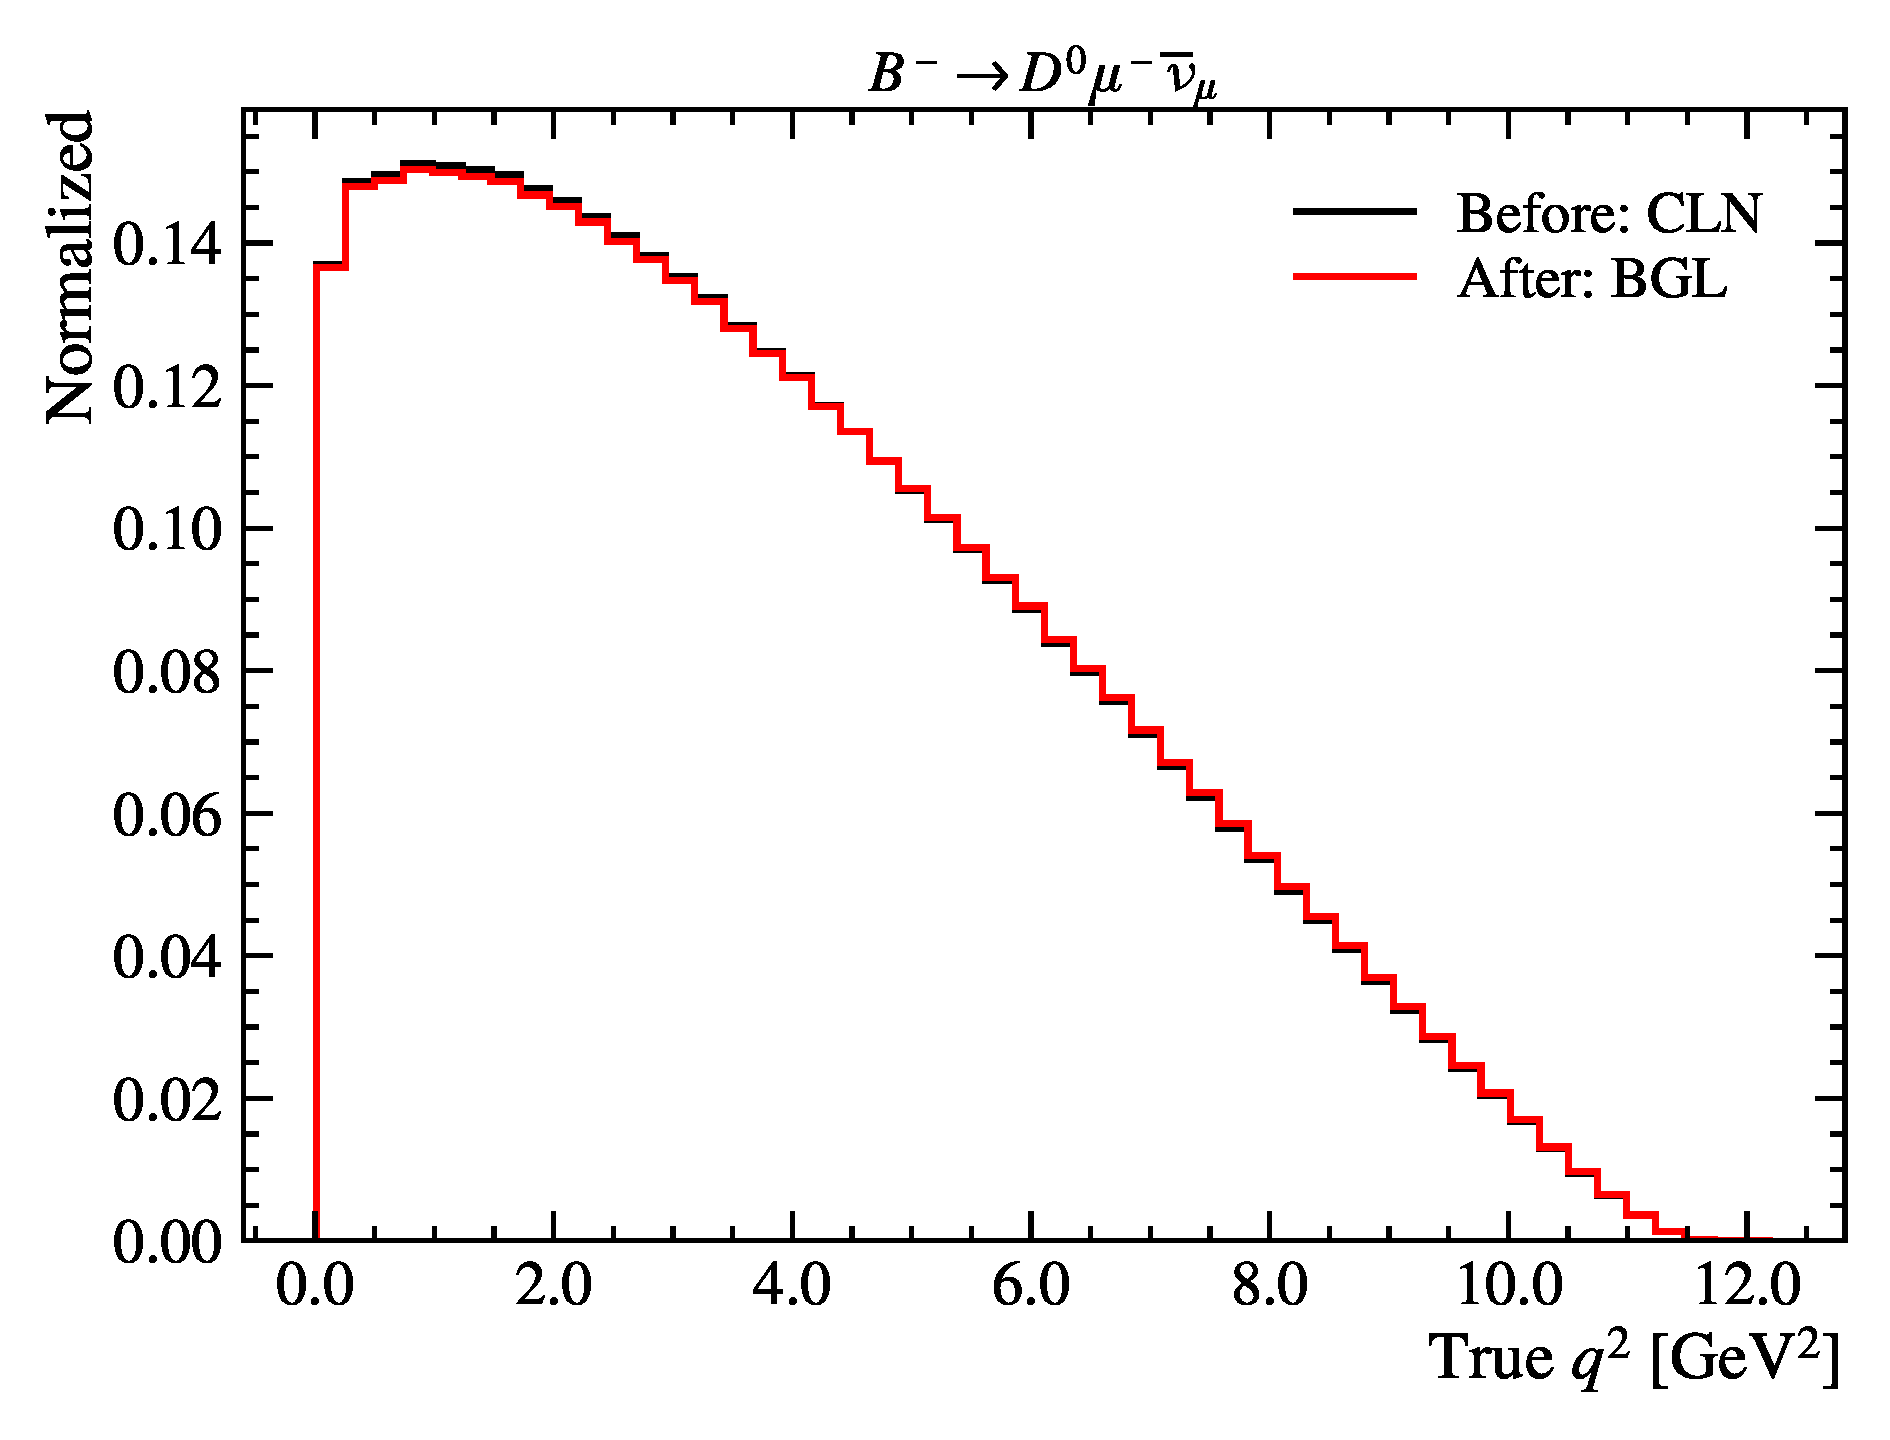
\includegraphics[width=0.45\textwidth]{
        ./figs-mc-correction/reweighting-form-factors/norm/D0Mu.pdf
    }
    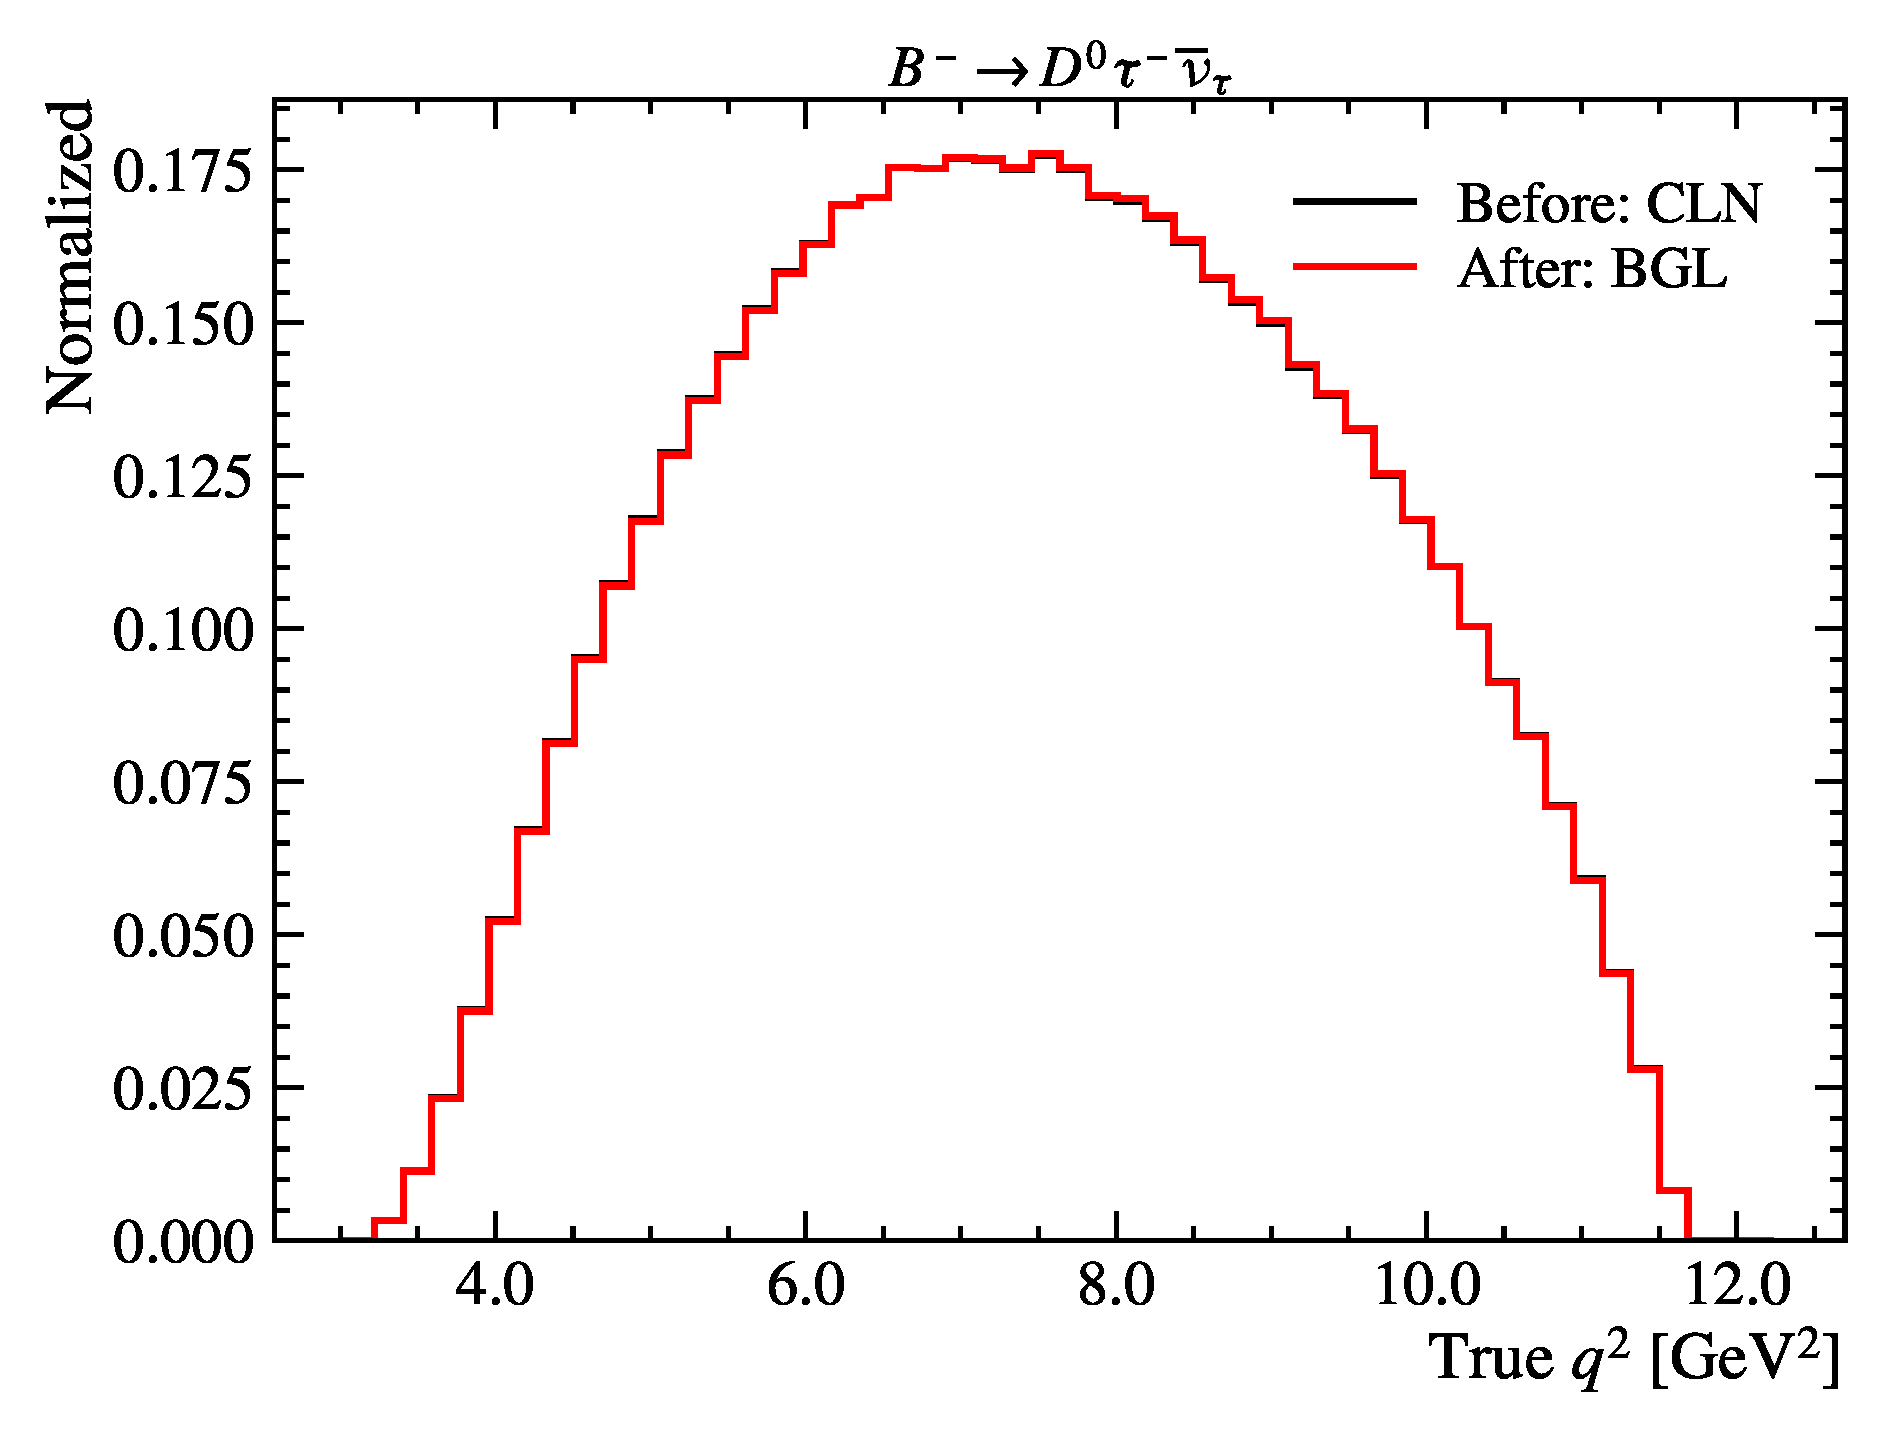
\includegraphics[width=0.45\textwidth]{
        ./figs-mc-correction/reweighting-form-factors/sig/D0Tau.pdf
    }
    \caption{
        Form factor reweight for $B \rightarrow \Dz \lepton\neulb$ MC samples.
    }
    \label{fig:ff-d0}
\end{figure}


\subsection{$B \rightarrow \Dstar$ decays}

The \Dstar MC samples are reweighted from a CLN to a BGL model with parameters
taken from the right-most column of Table XII in the \textbf{v1} version of
\cite{Bazavov_2021},
the first work to calculate \Dstar form factors at non-zero recoil
based on lattice-QCD with constraints from external measurements.
The change of true \qSq is shown in \cref{fig:ff-dst}.

The $c_3$ and $d_2$ parameters are not implemented in \Hammer (yet).
Given the large uncertainties on these sub-dominate parameters,
they are set to 0 with the corresponding entries in the correlation matrix
removed.

\begin{figure}[htb]
    \centering
    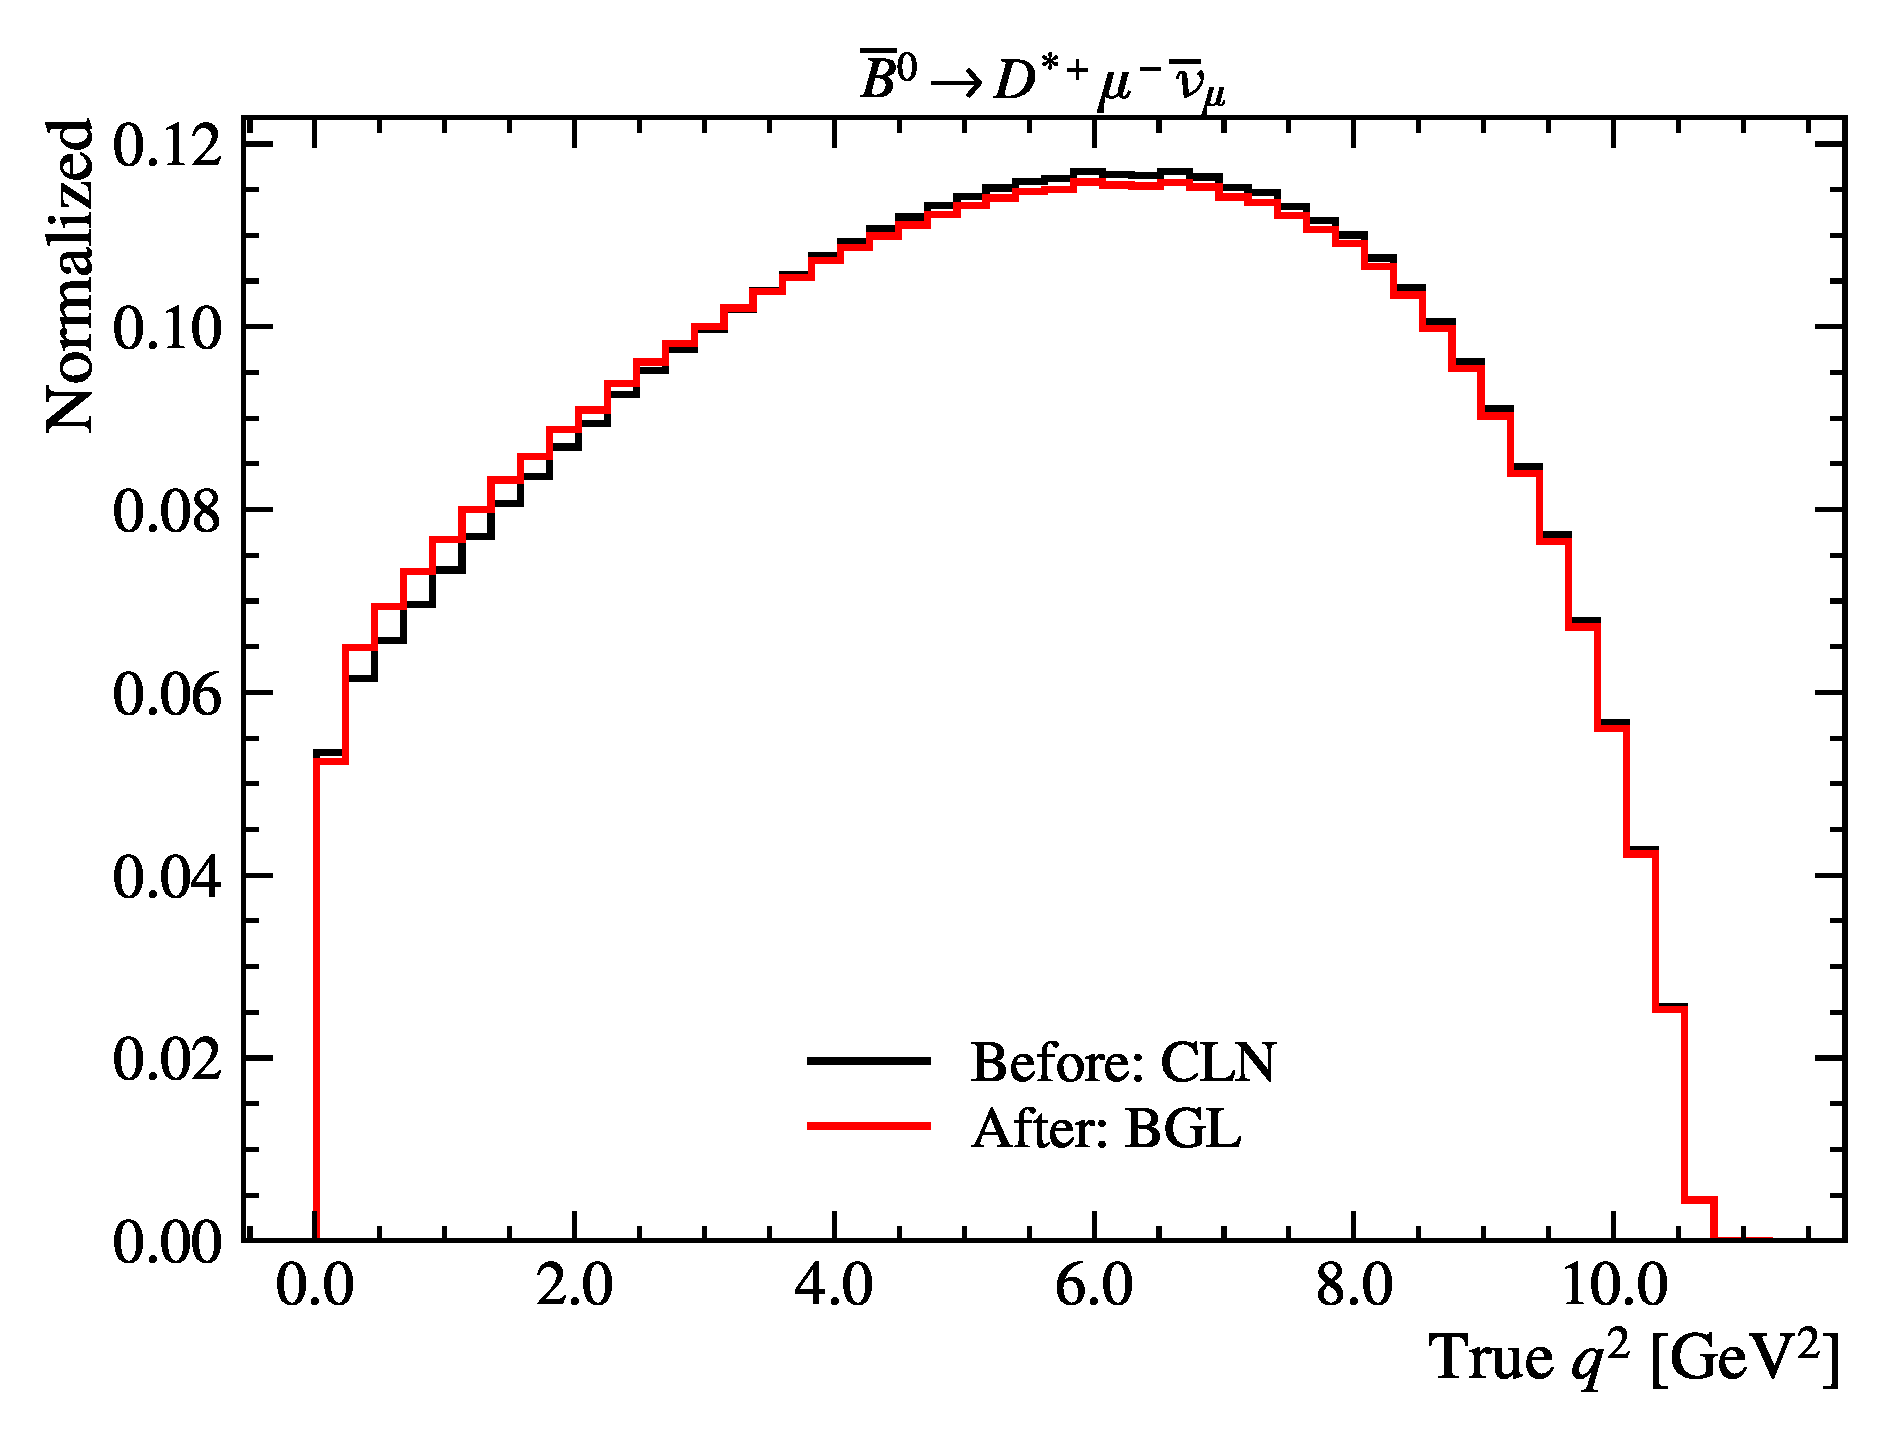
\includegraphics[width=0.45\textwidth]{
        ./figs-mc-correction/reweighting-form-factors/norm/DstMu.pdf
    }
    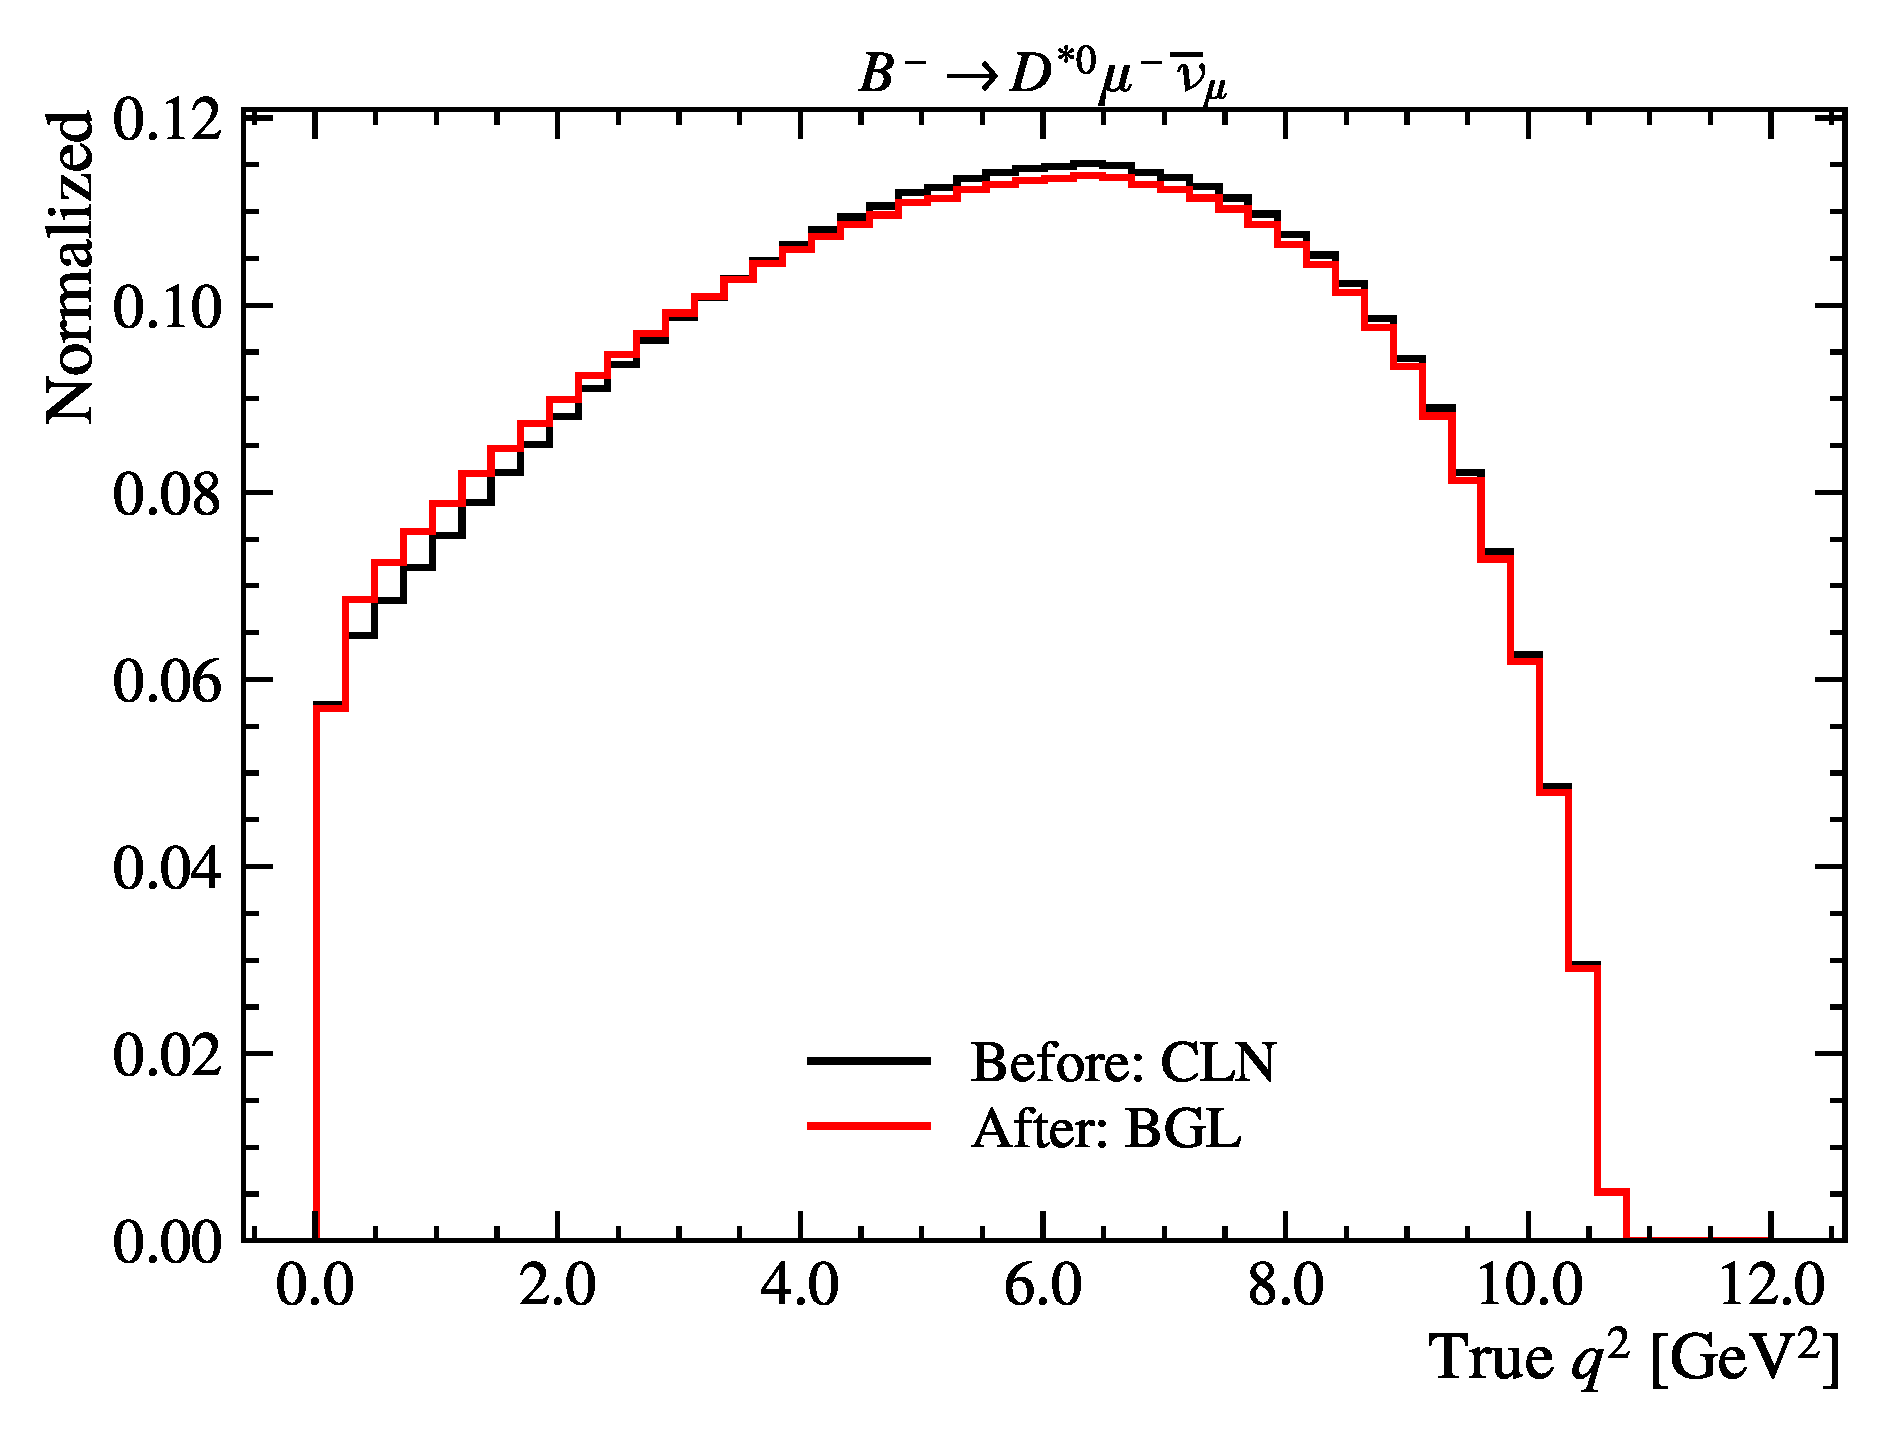
\includegraphics[width=0.45\textwidth]{
        ./figs-mc-correction/reweighting-form-factors/norm/Dst0Mu.pdf
    }

    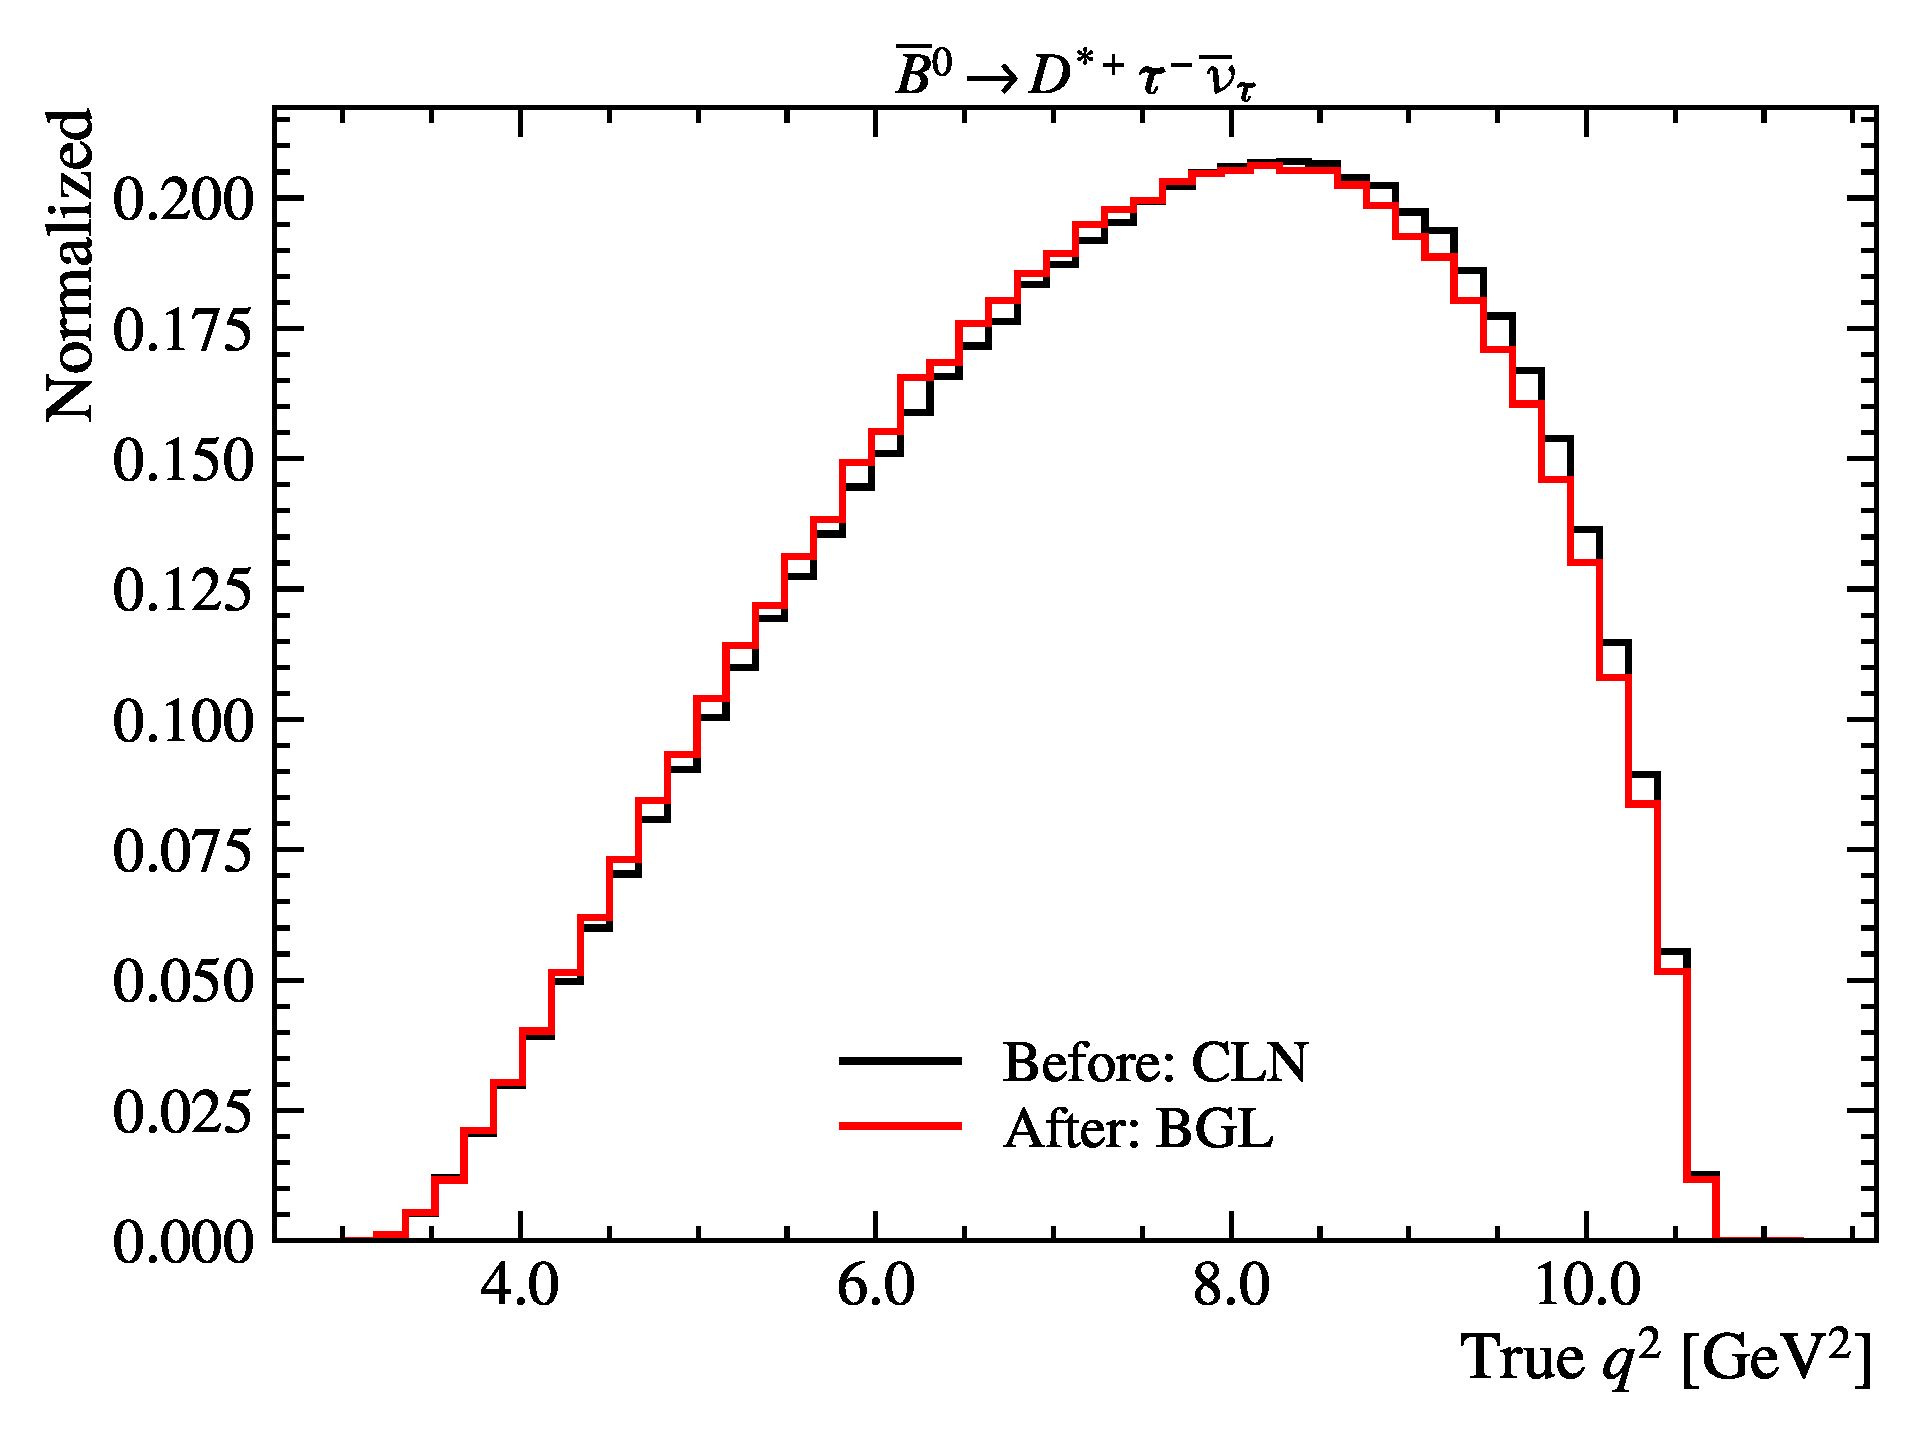
\includegraphics[width=0.45\textwidth]{
        ./figs-mc-correction/reweighting-form-factors/sig/DstTau.pdf
    }
    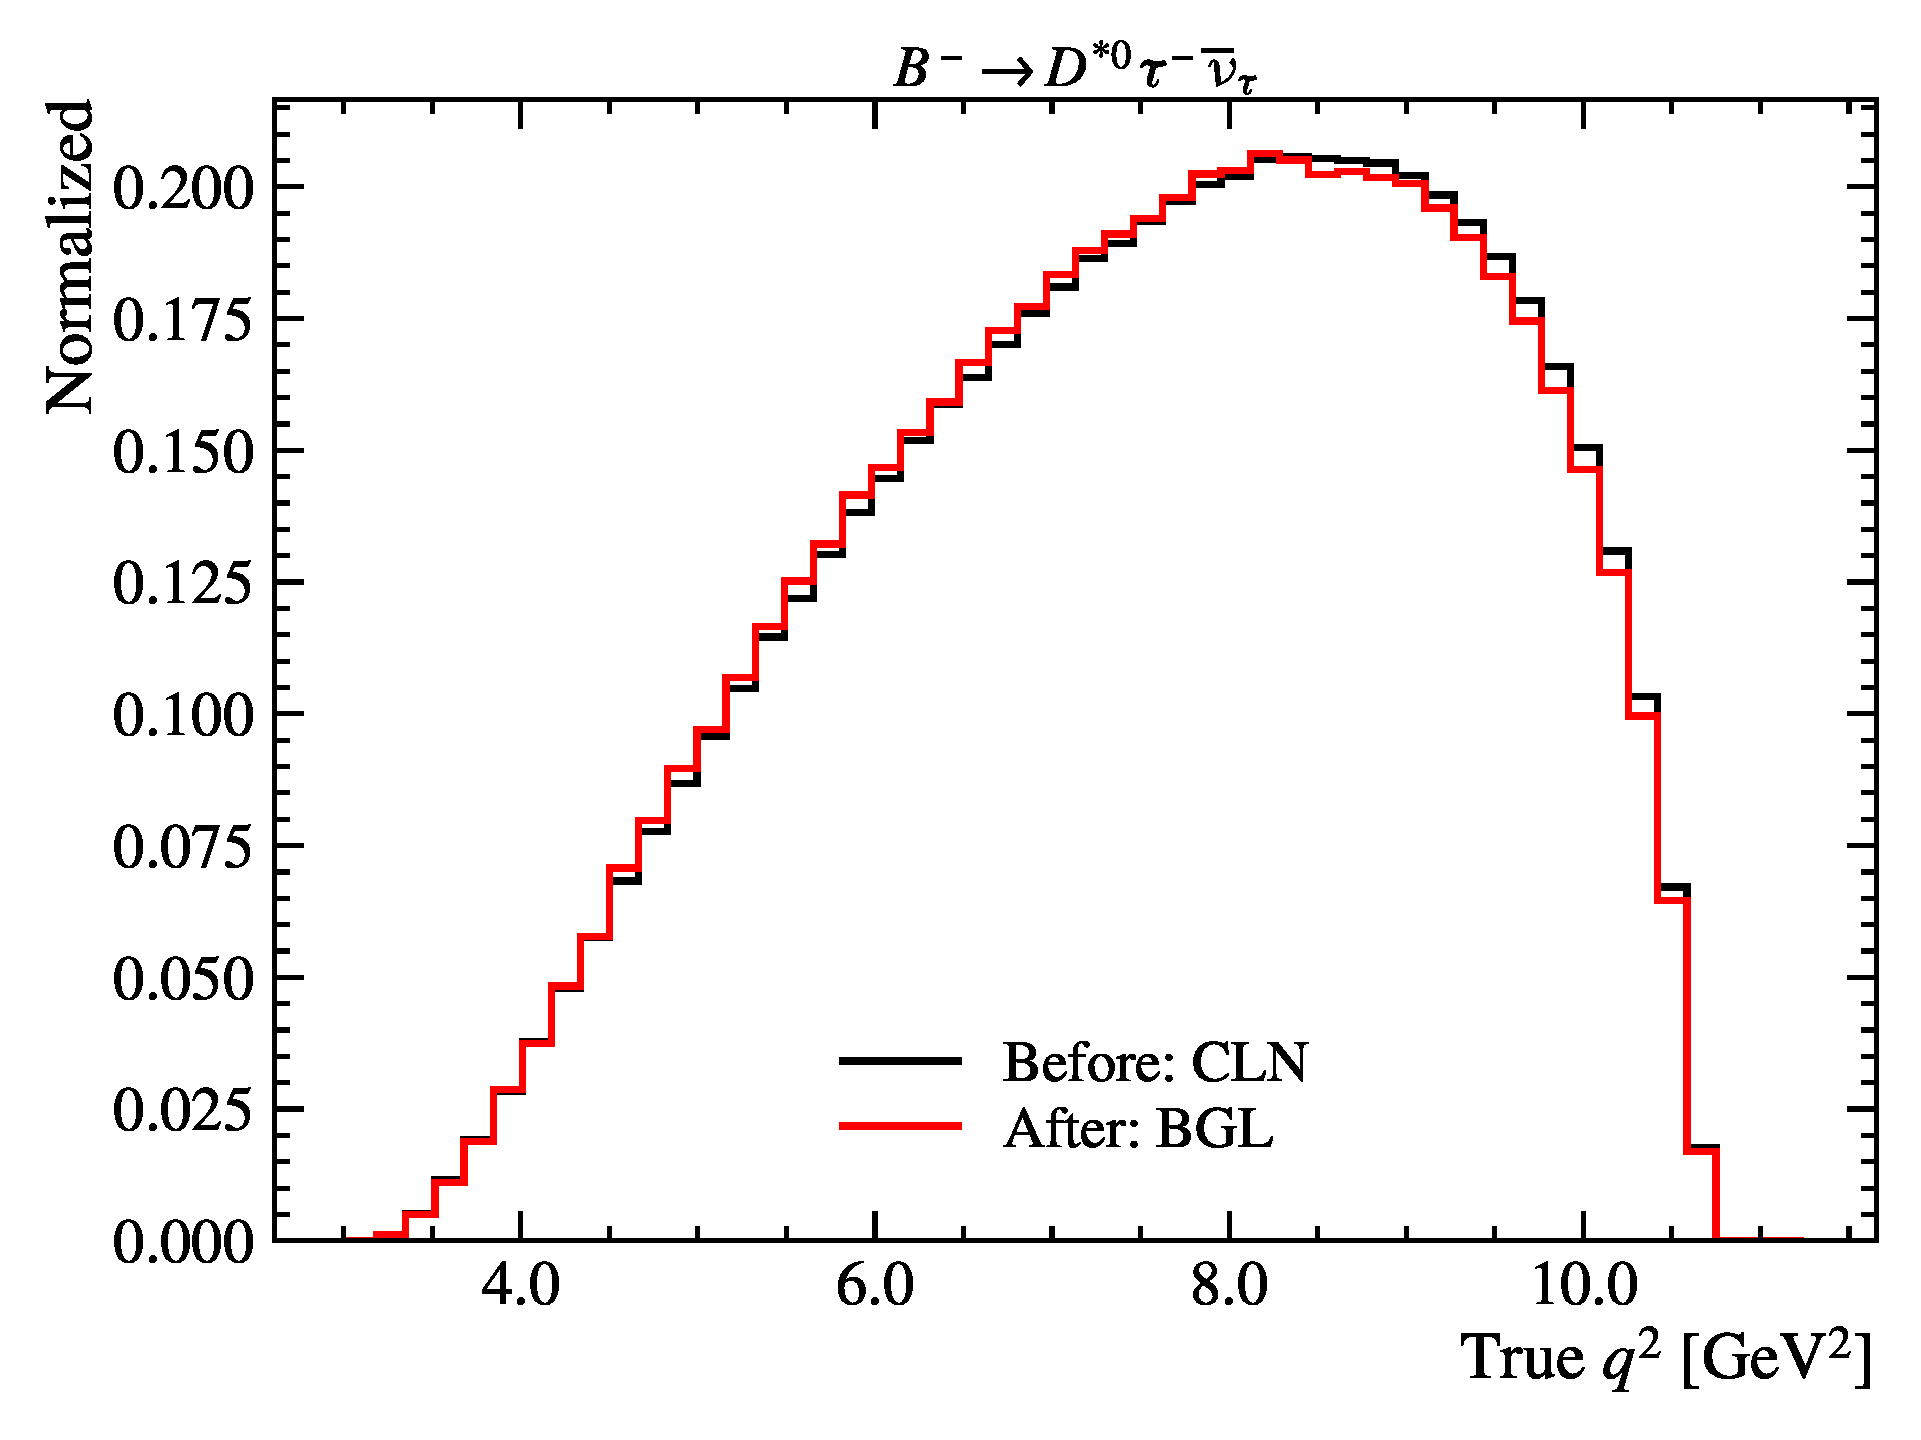
\includegraphics[width=0.45\textwidth]{
        ./figs-mc-correction/reweighting-form-factors/sig/Dst0Tau.pdf
    }
    \caption{
        Form factor reweight for $B \rightarrow \D^* \lepton\neulb$ MC samples.
    }
    \label{fig:ff-dst}
\end{figure}


\subsection{$B \rightarrow \Dstst$ decays}

The four 1P \Dstst states ($D^*_0$, $D_1$, $D'_1$, $D^*_2$) with decay mode
$B \rightarrow D^{**}\lepton\neulb$,
generated with ISGW2 form factor model,
are reweighted to BLR model.
These \Dstst states can be further split into two heavy quark spin symmetry
doublets: $D^{1/2+} (D^*_0, D'_1)$ and $D^{3/2+}: (D_1, D^*_2)$.
The BLR parameters for the doublets are taken from Table V of
\cite{Bernlochner_2018}.

The form factor parameters are allowed to float in the fit from the nominal
values, with the shift of fit variables due to these parameters accounted for
via an interpolation/extrapolation mechanism\footnote{
    % FIXME: Implement the ref
    More details regarding the interpolation/extrapolation are discussed
    in \cref{ref:fit:var}.
}.
Uniquely for $D^{**}$, the fitted parameters have large deviations from the
nominal (up to $7\sigma$!), at which point the extrapolation becomes
unphysical.
Similar effect has been reported in the previous analysis.

To workaround the large deviations from nominal, the \emph{nominal} values for
$D^{**}$ form factor parameters are \emph{shifted} based on the fit, so that
the deviations are small ($\leq 2\sigma$) and the
interpolation/extrapolation remains physical.
The change of true \qSq with the \emph{shifted} parameters are
plotted in \cref{fig:ff-rwt-Dstst-norm-like,fig:ff-rwt-Dstst-sig-like},
which are used in the fit as the nominal.
The change of fit variables with the parameters taken from
\cite{Bernlochner_2018} are plotted separately in
\cref{fig:ff-rwt-raw-Dstst-norm-like,fig:ff-rwt-raw-Dstst-sig-like}.

\begin{figure}[ht]
    \centering
    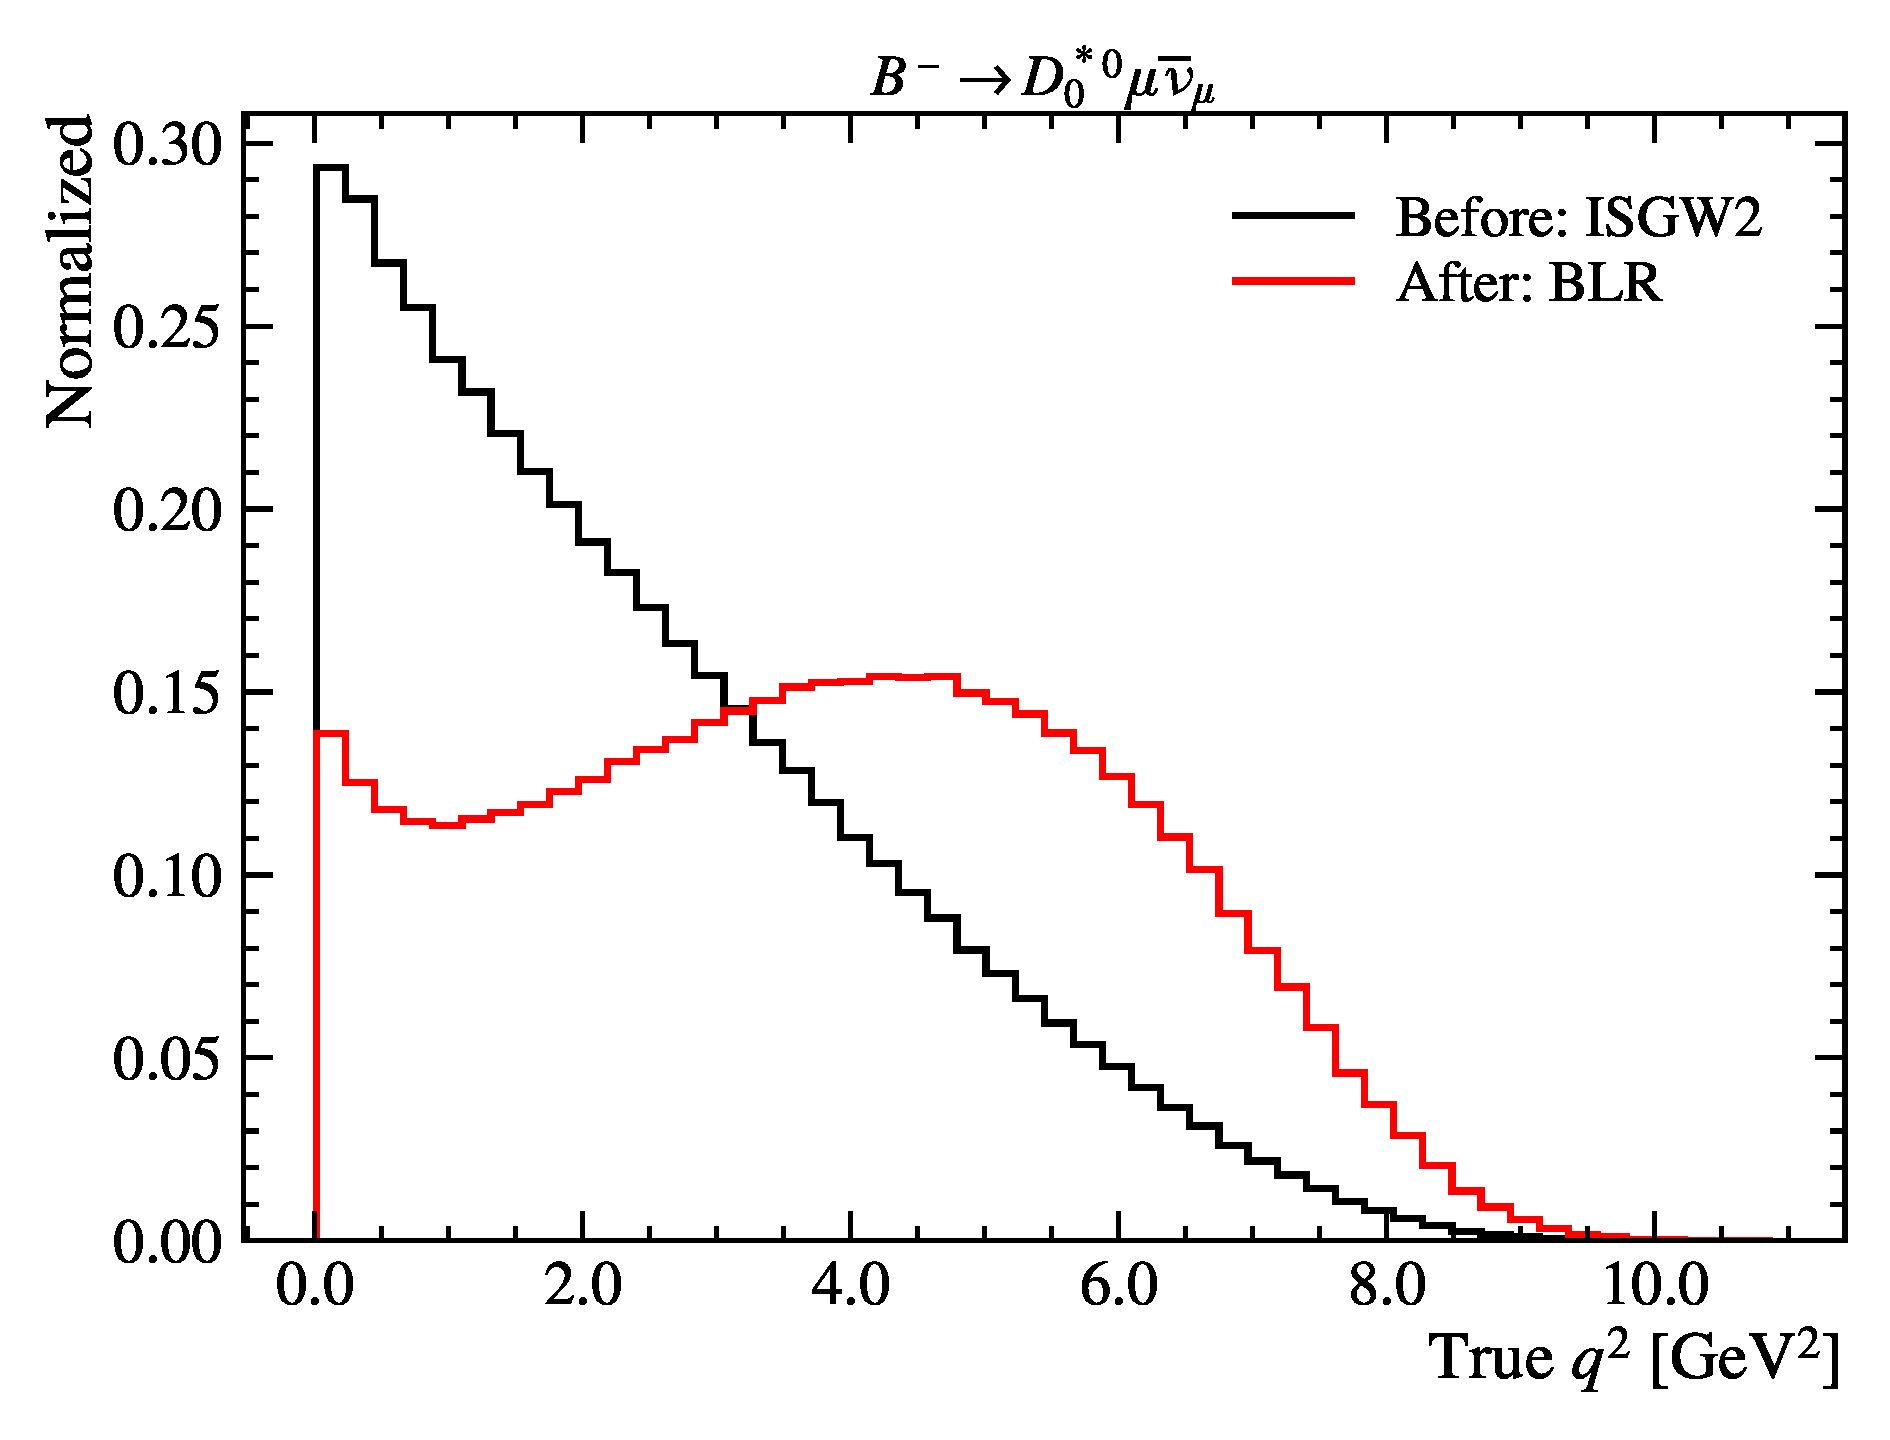
\includegraphics[width=0.24\textwidth]{
        ./figs-mc-correction/reweighting-form-factors/DststMu/D0stst0Mu.pdf
    }
    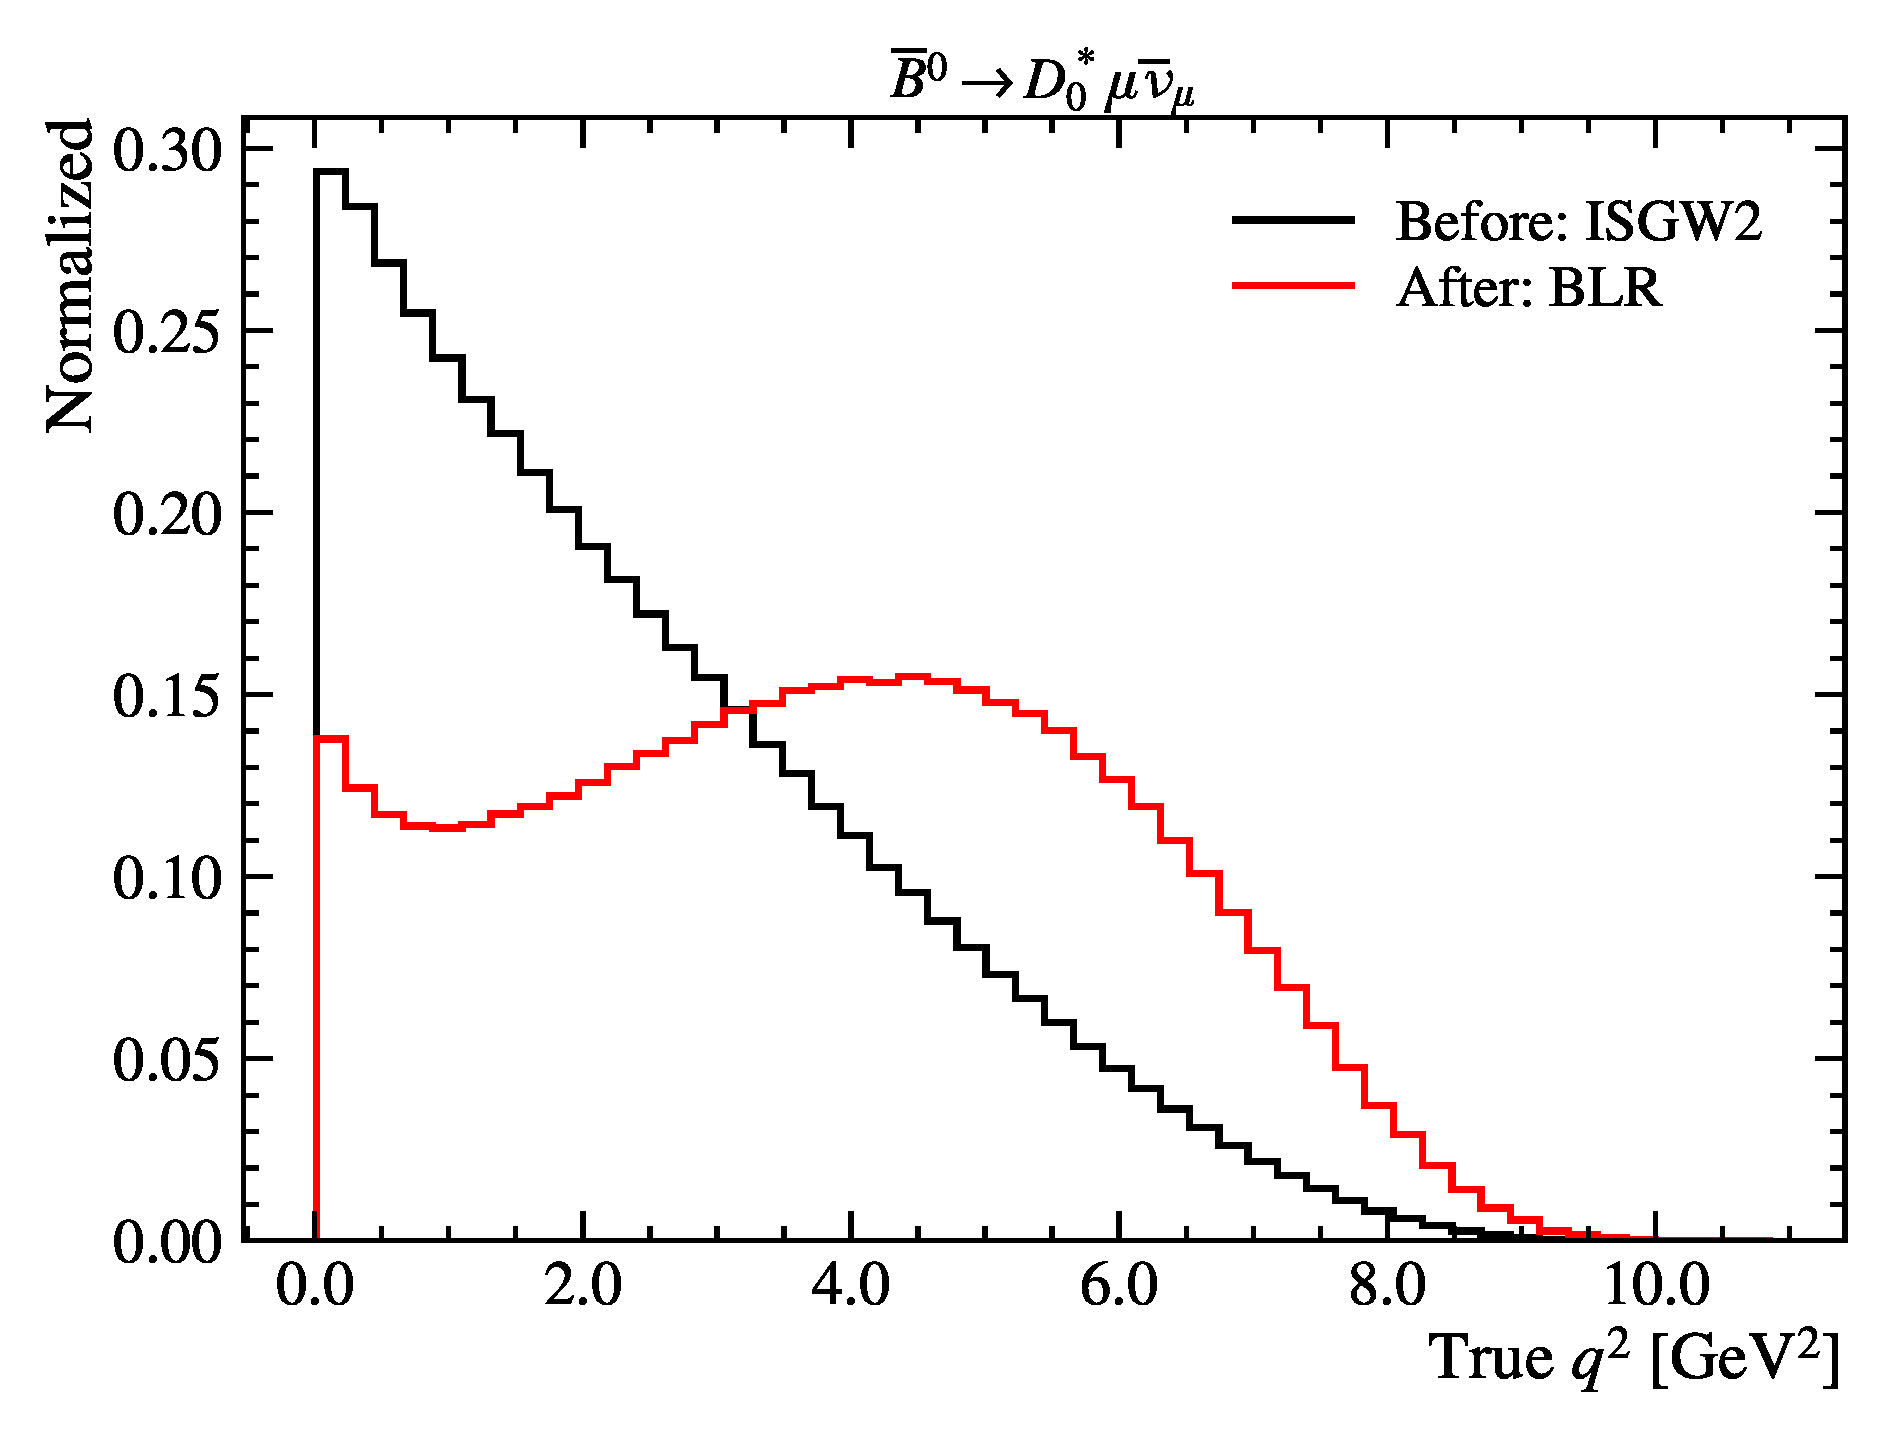
\includegraphics[width=0.24\textwidth]{
        ./figs-mc-correction/reweighting-form-factors/DststMu/D0ststMu.pdf
    }
    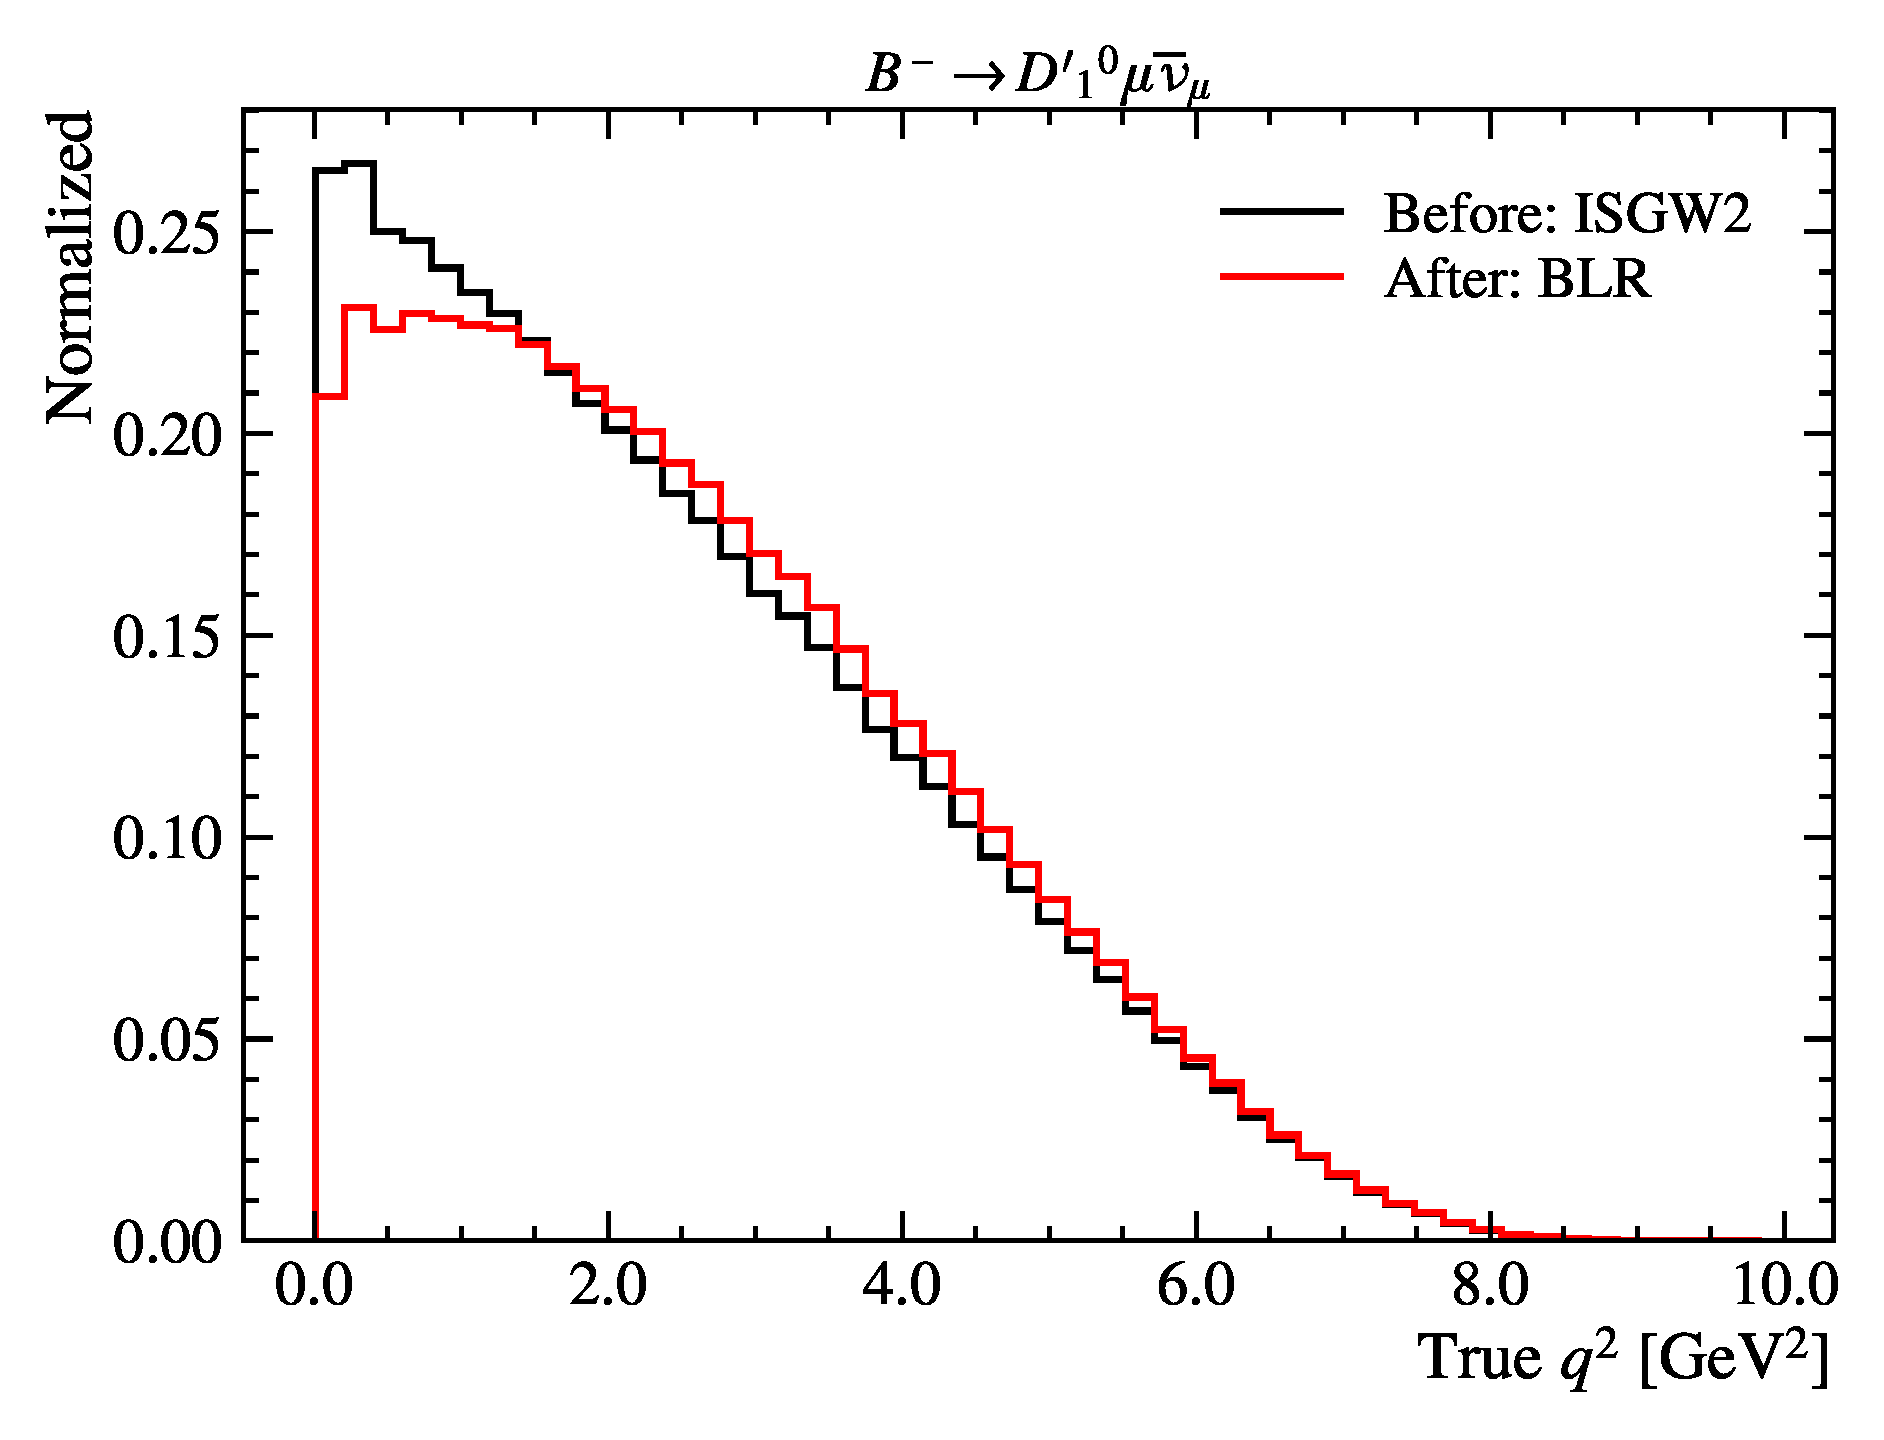
\includegraphics[width=0.24\textwidth]{
        ./figs-mc-correction/reweighting-form-factors/DststMu/D1pstst0Mu.pdf
    }
    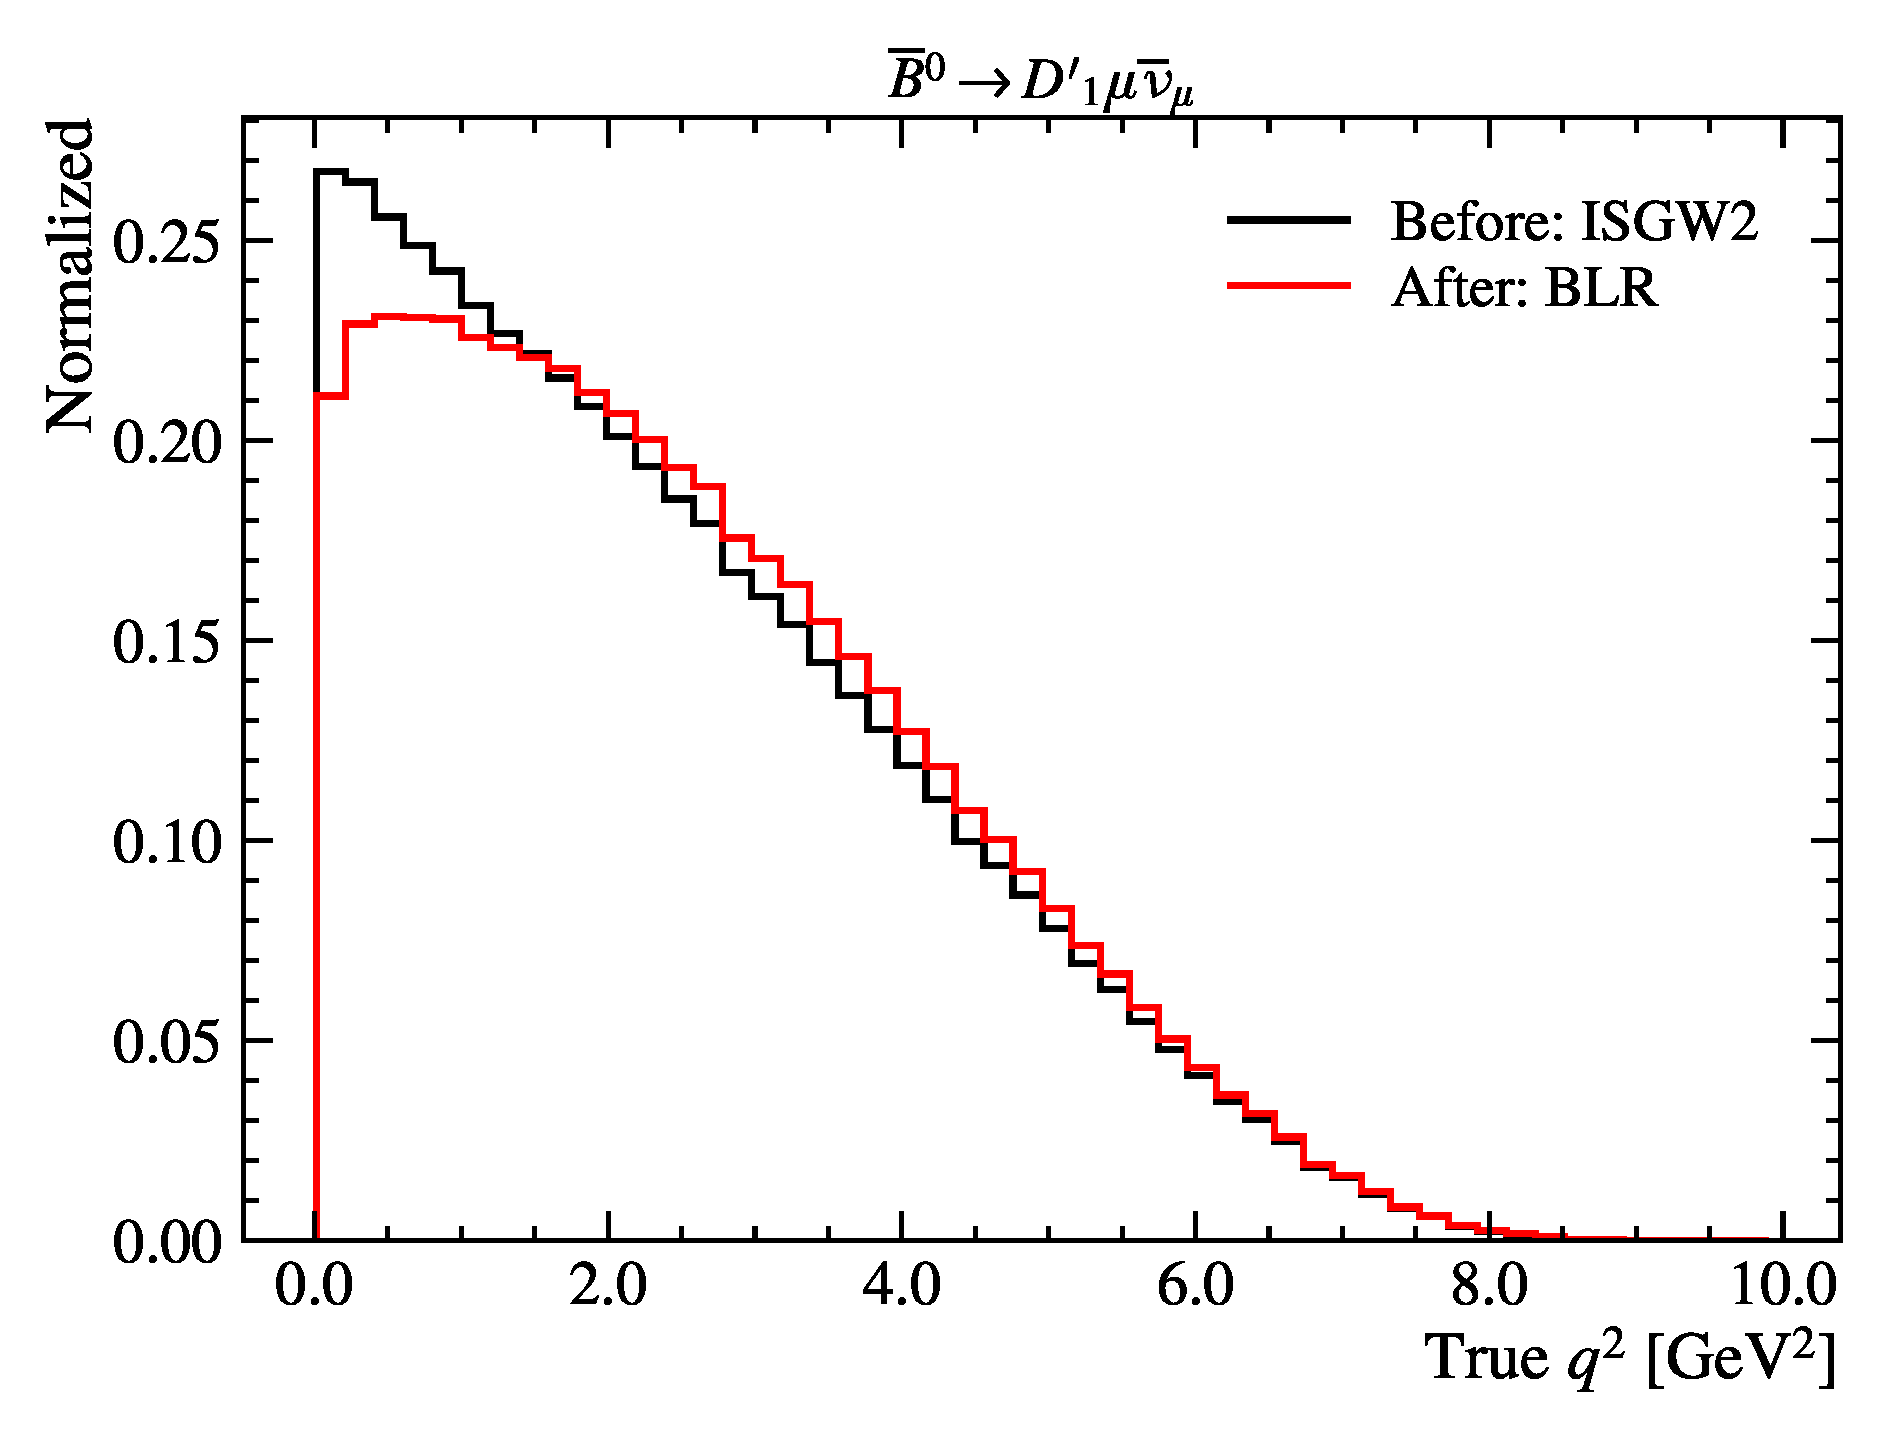
\includegraphics[width=0.24\textwidth]{
        ./figs-mc-correction/reweighting-form-factors/DststMu/D1pststMu.pdf
    }

    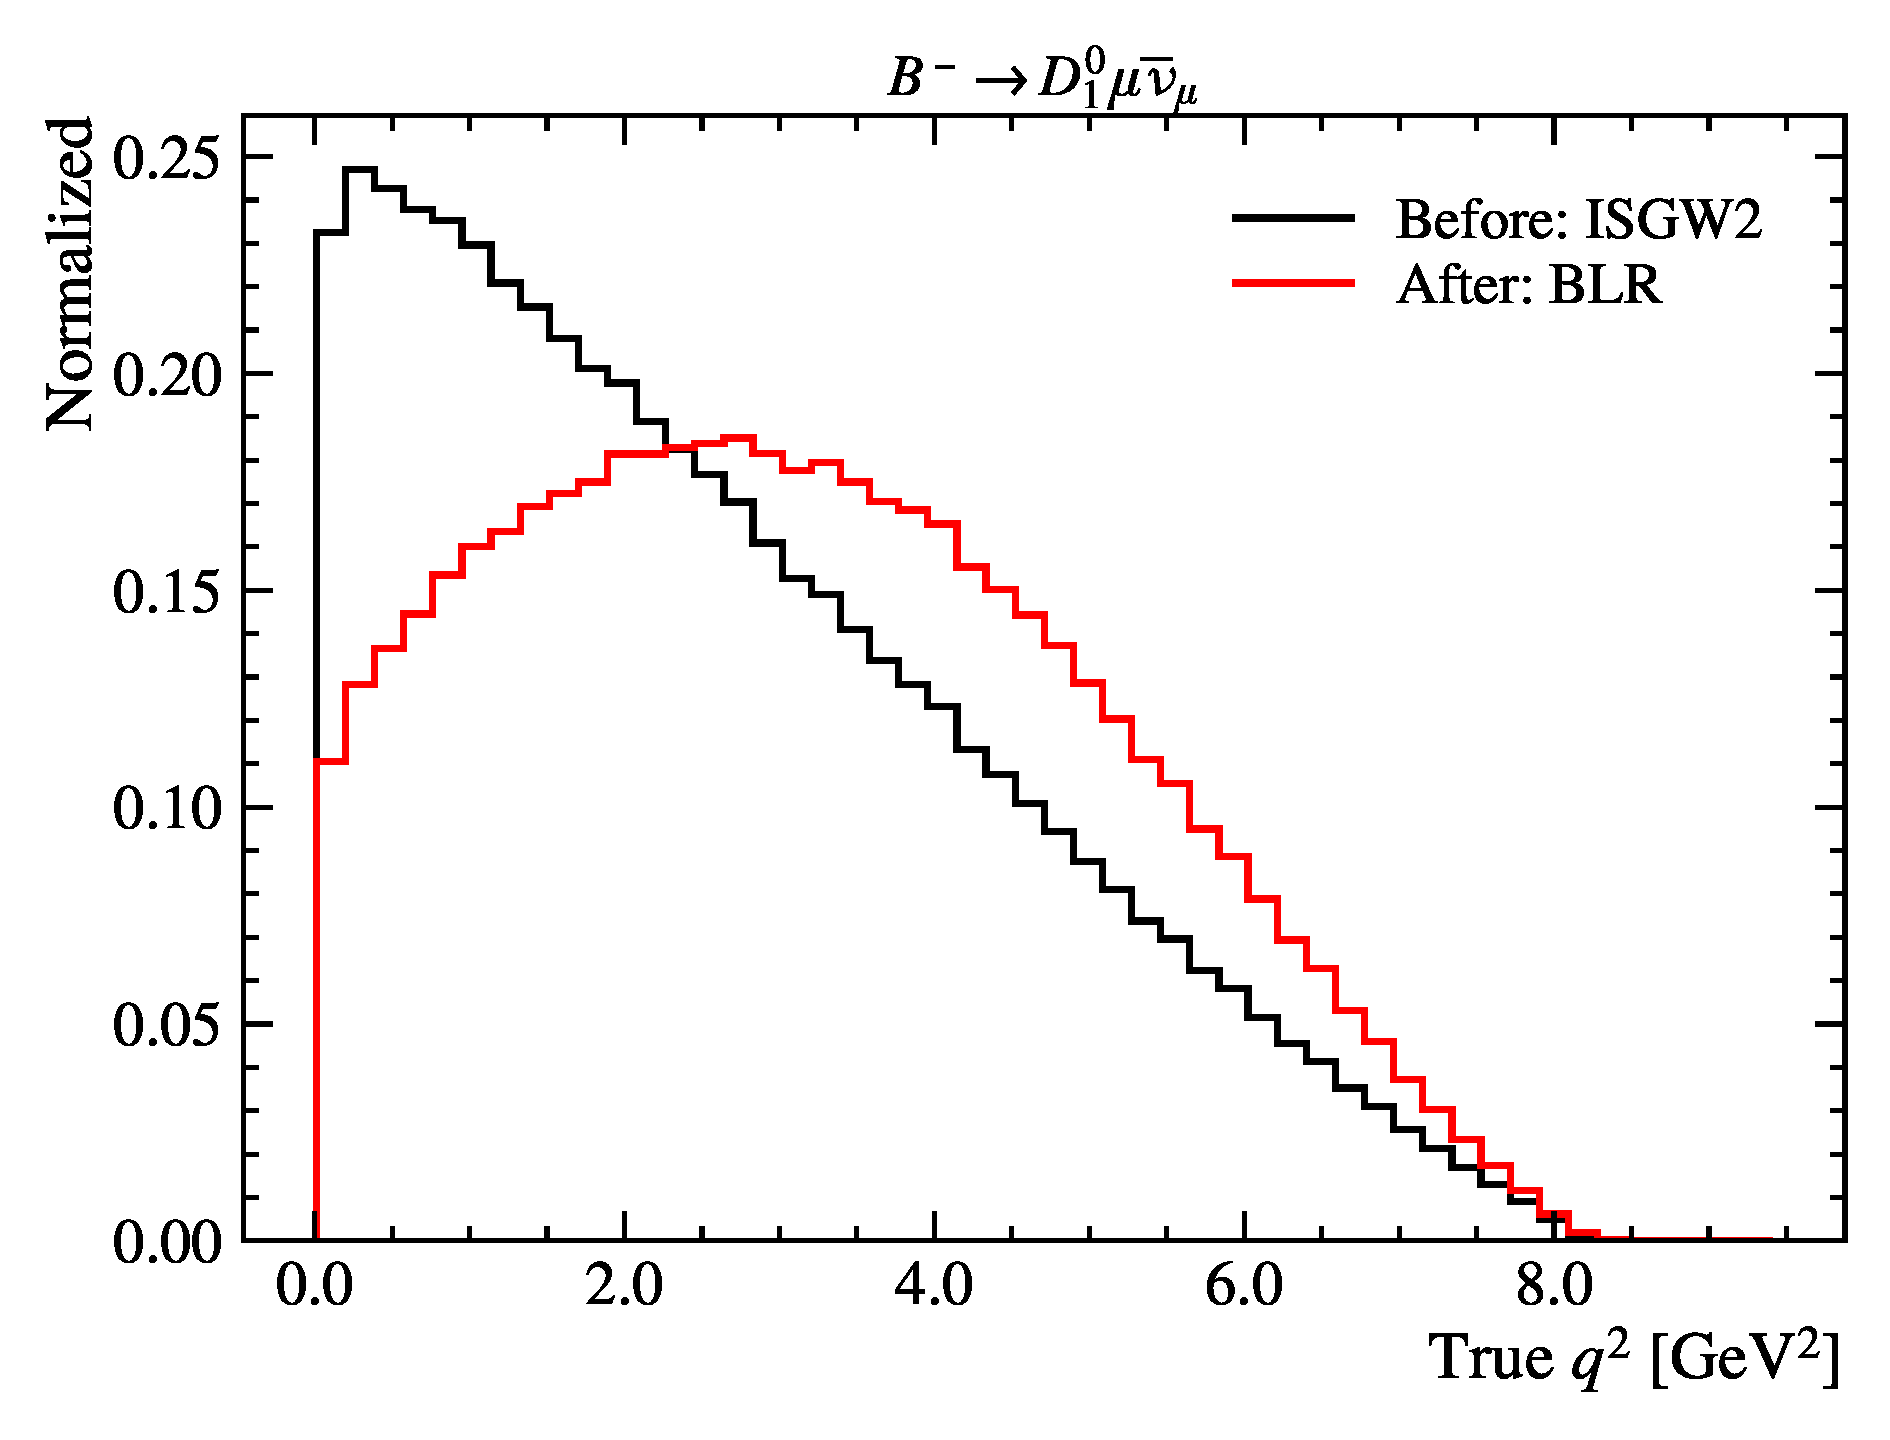
\includegraphics[width=0.24\textwidth]{
        ./figs-mc-correction/reweighting-form-factors/DststMu/D1stst0Mu.pdf
    }
    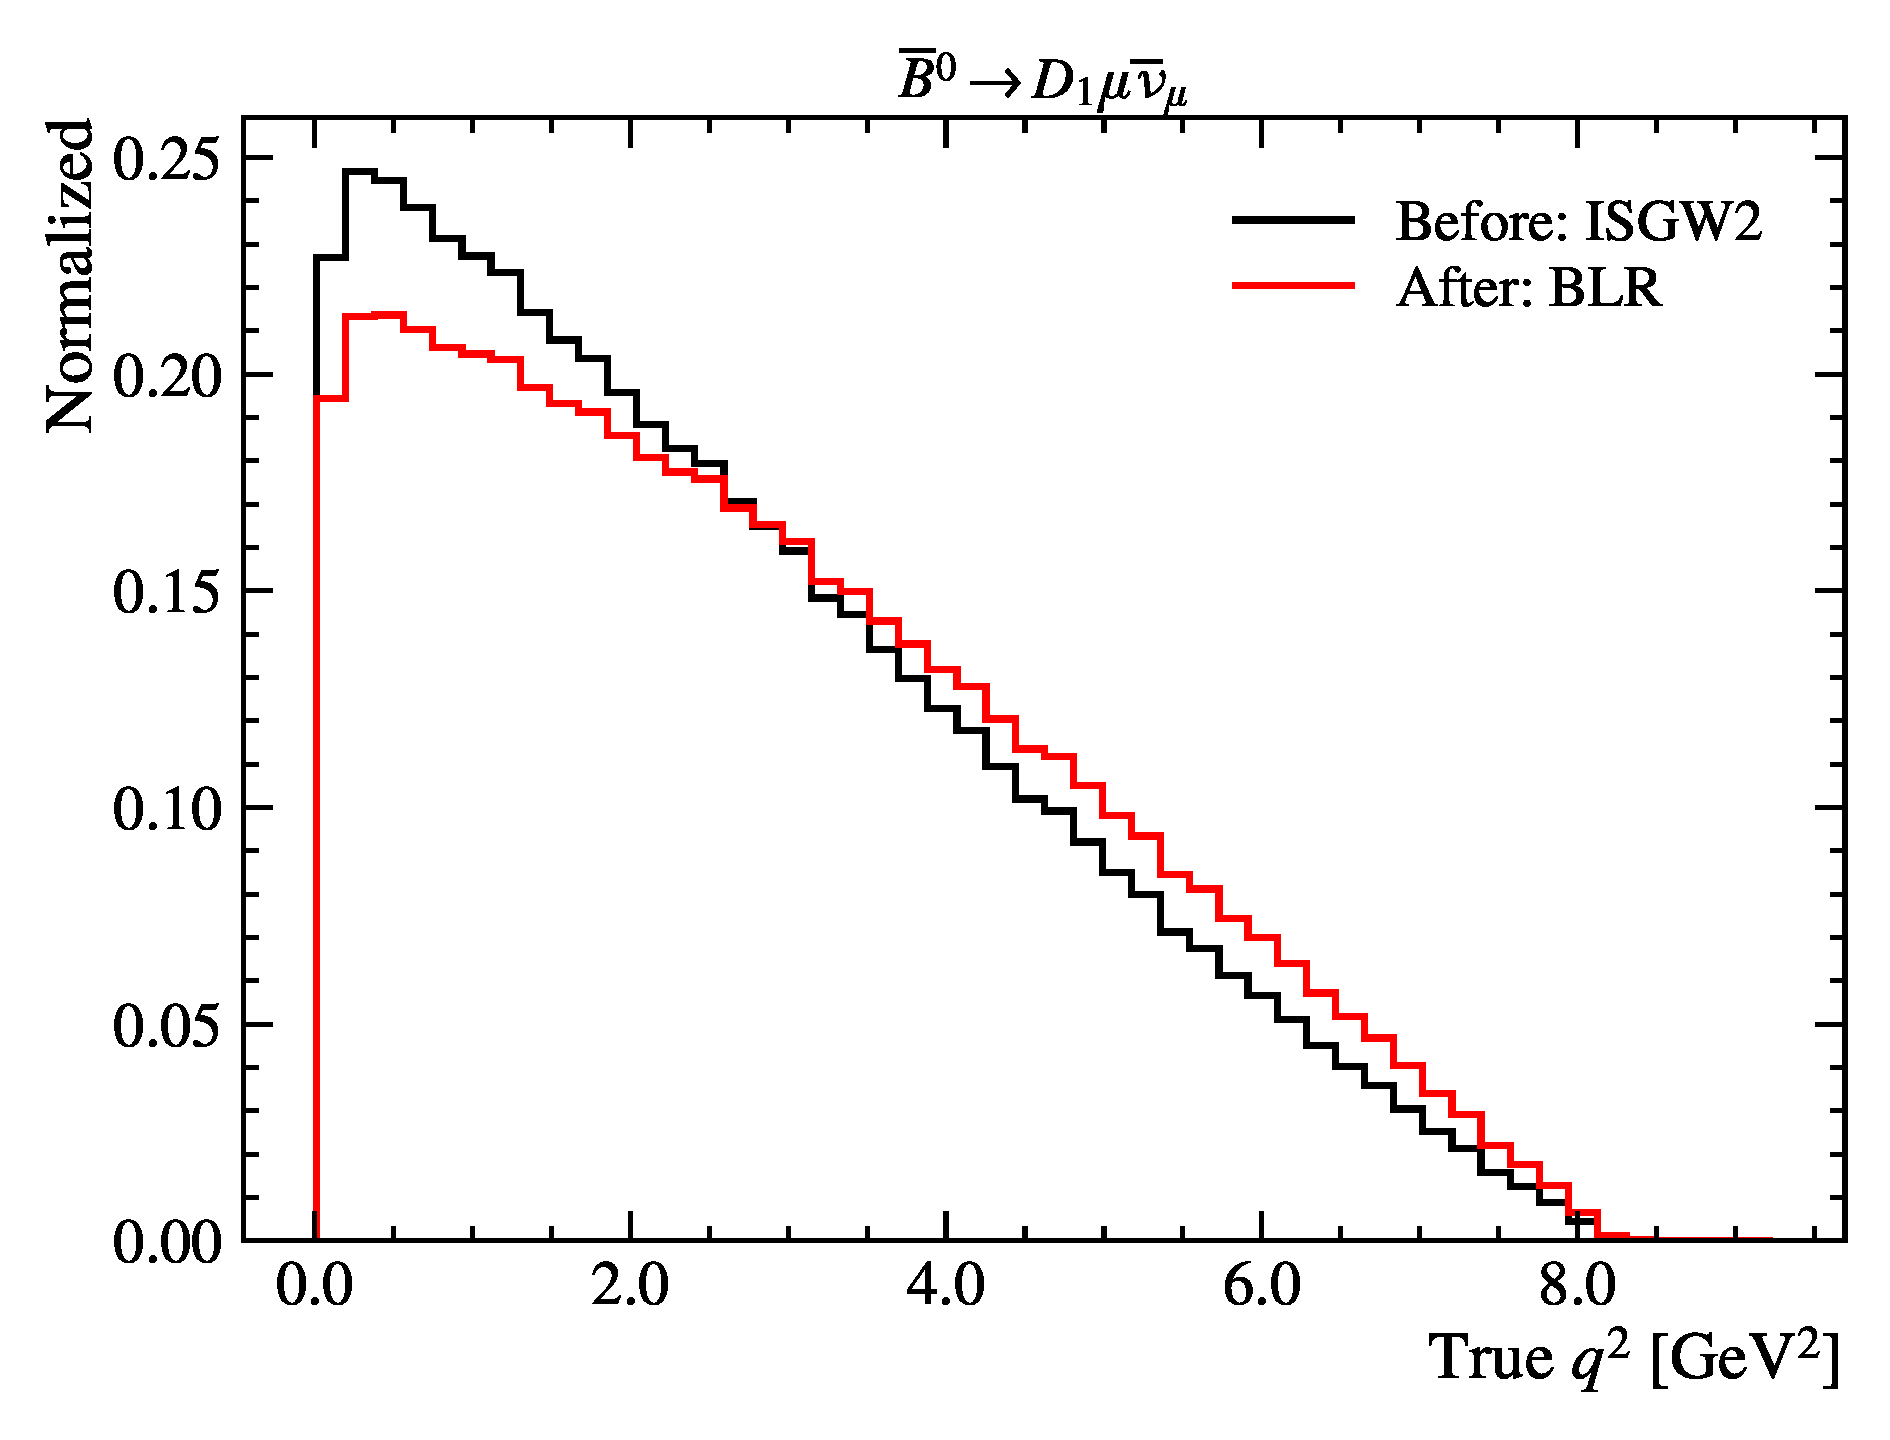
\includegraphics[width=0.24\textwidth]{
        ./figs-mc-correction/reweighting-form-factors/DststMu/D1ststMu.pdf
    }
    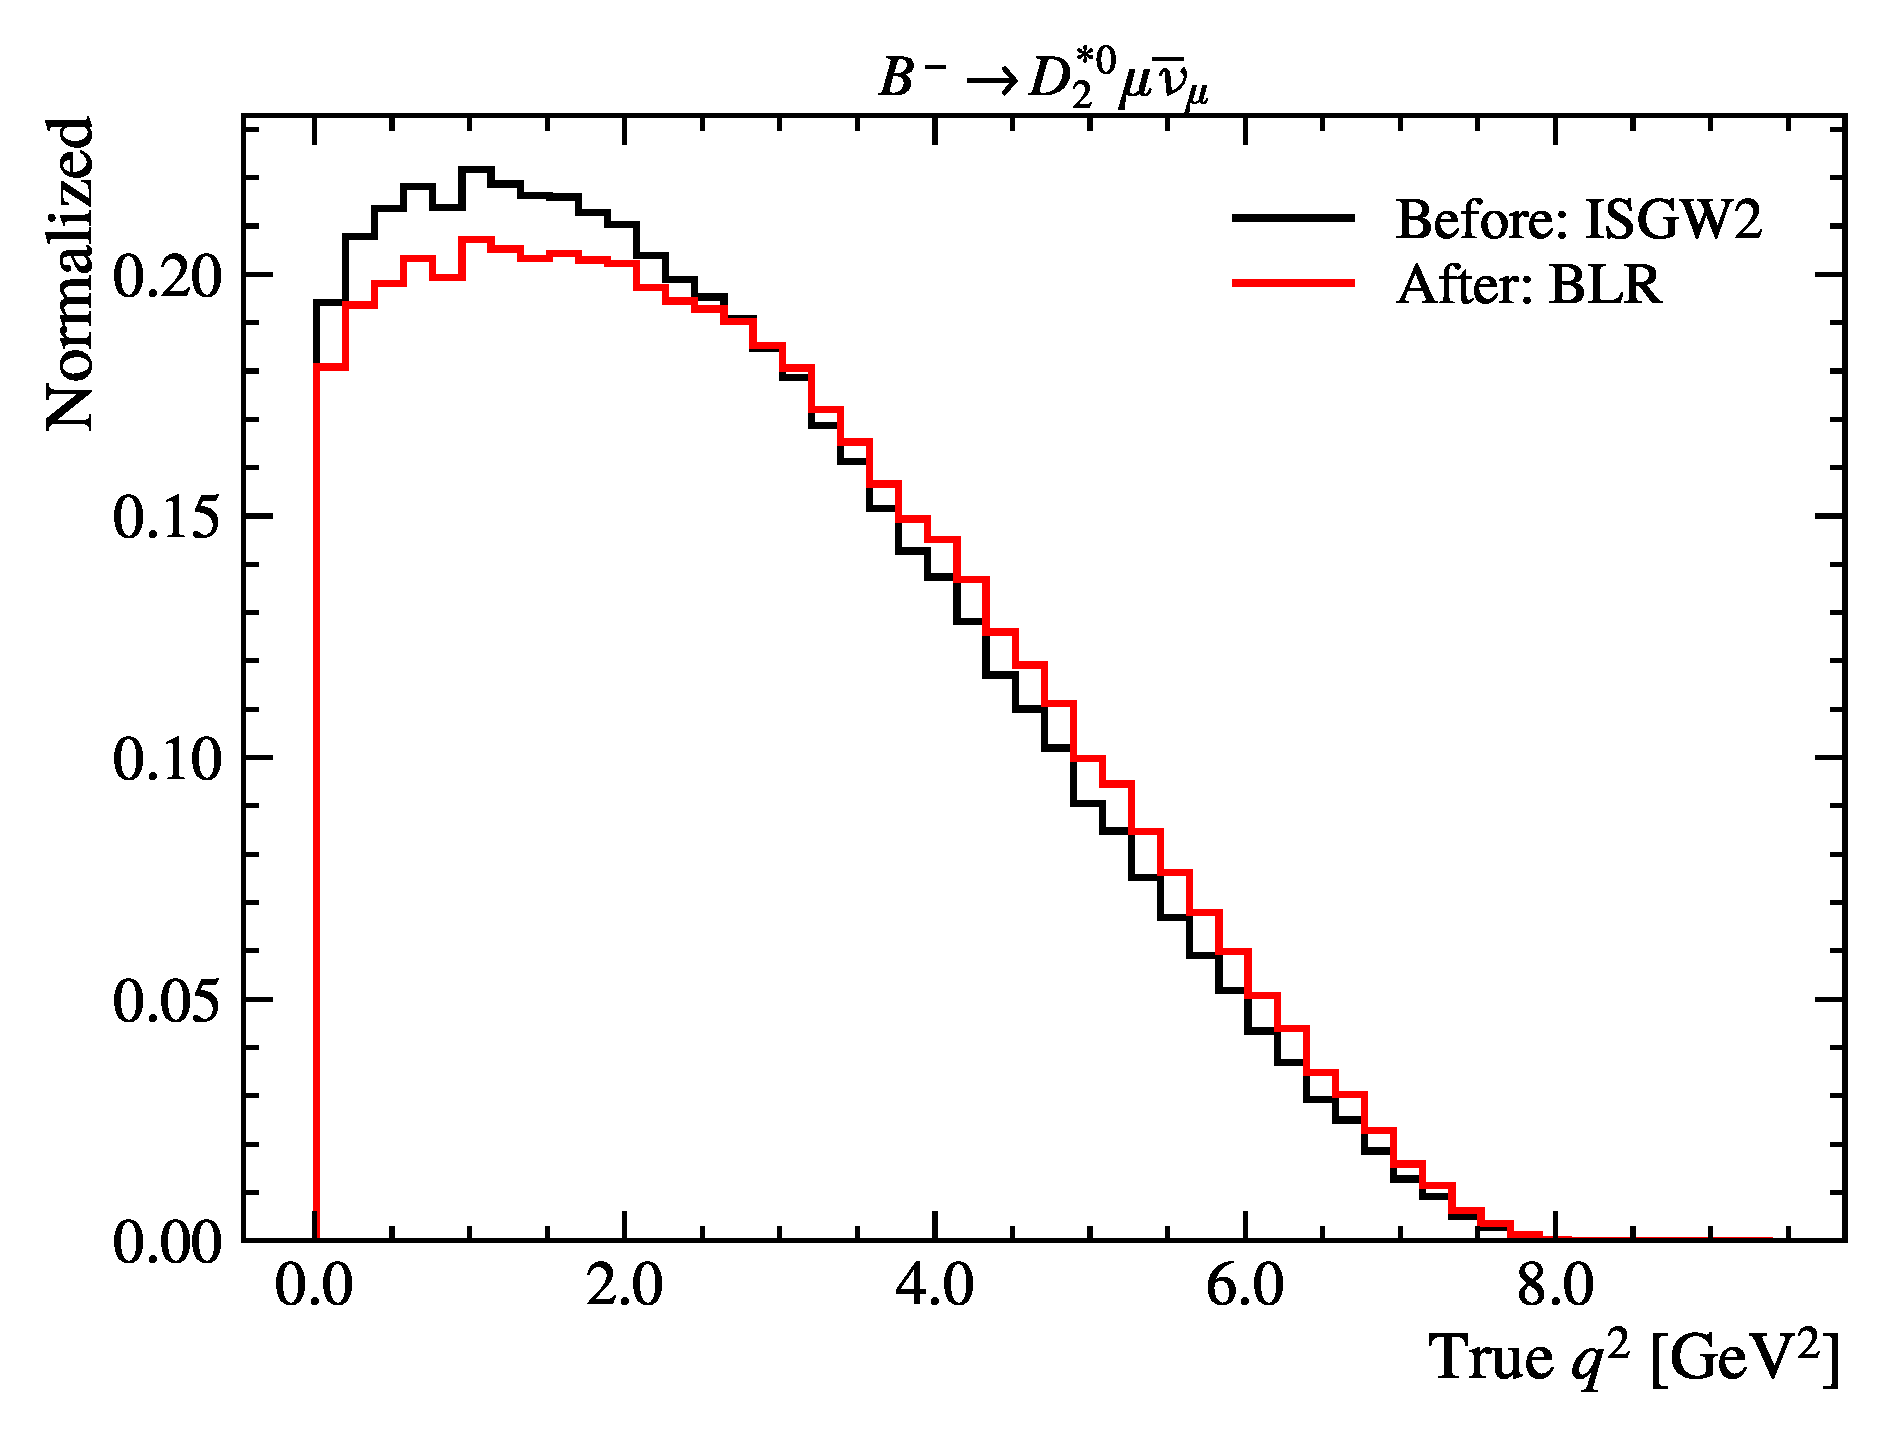
\includegraphics[width=0.24\textwidth]{
        ./figs-mc-correction/reweighting-form-factors/DststMu/D2stst0Mu.pdf
    }
    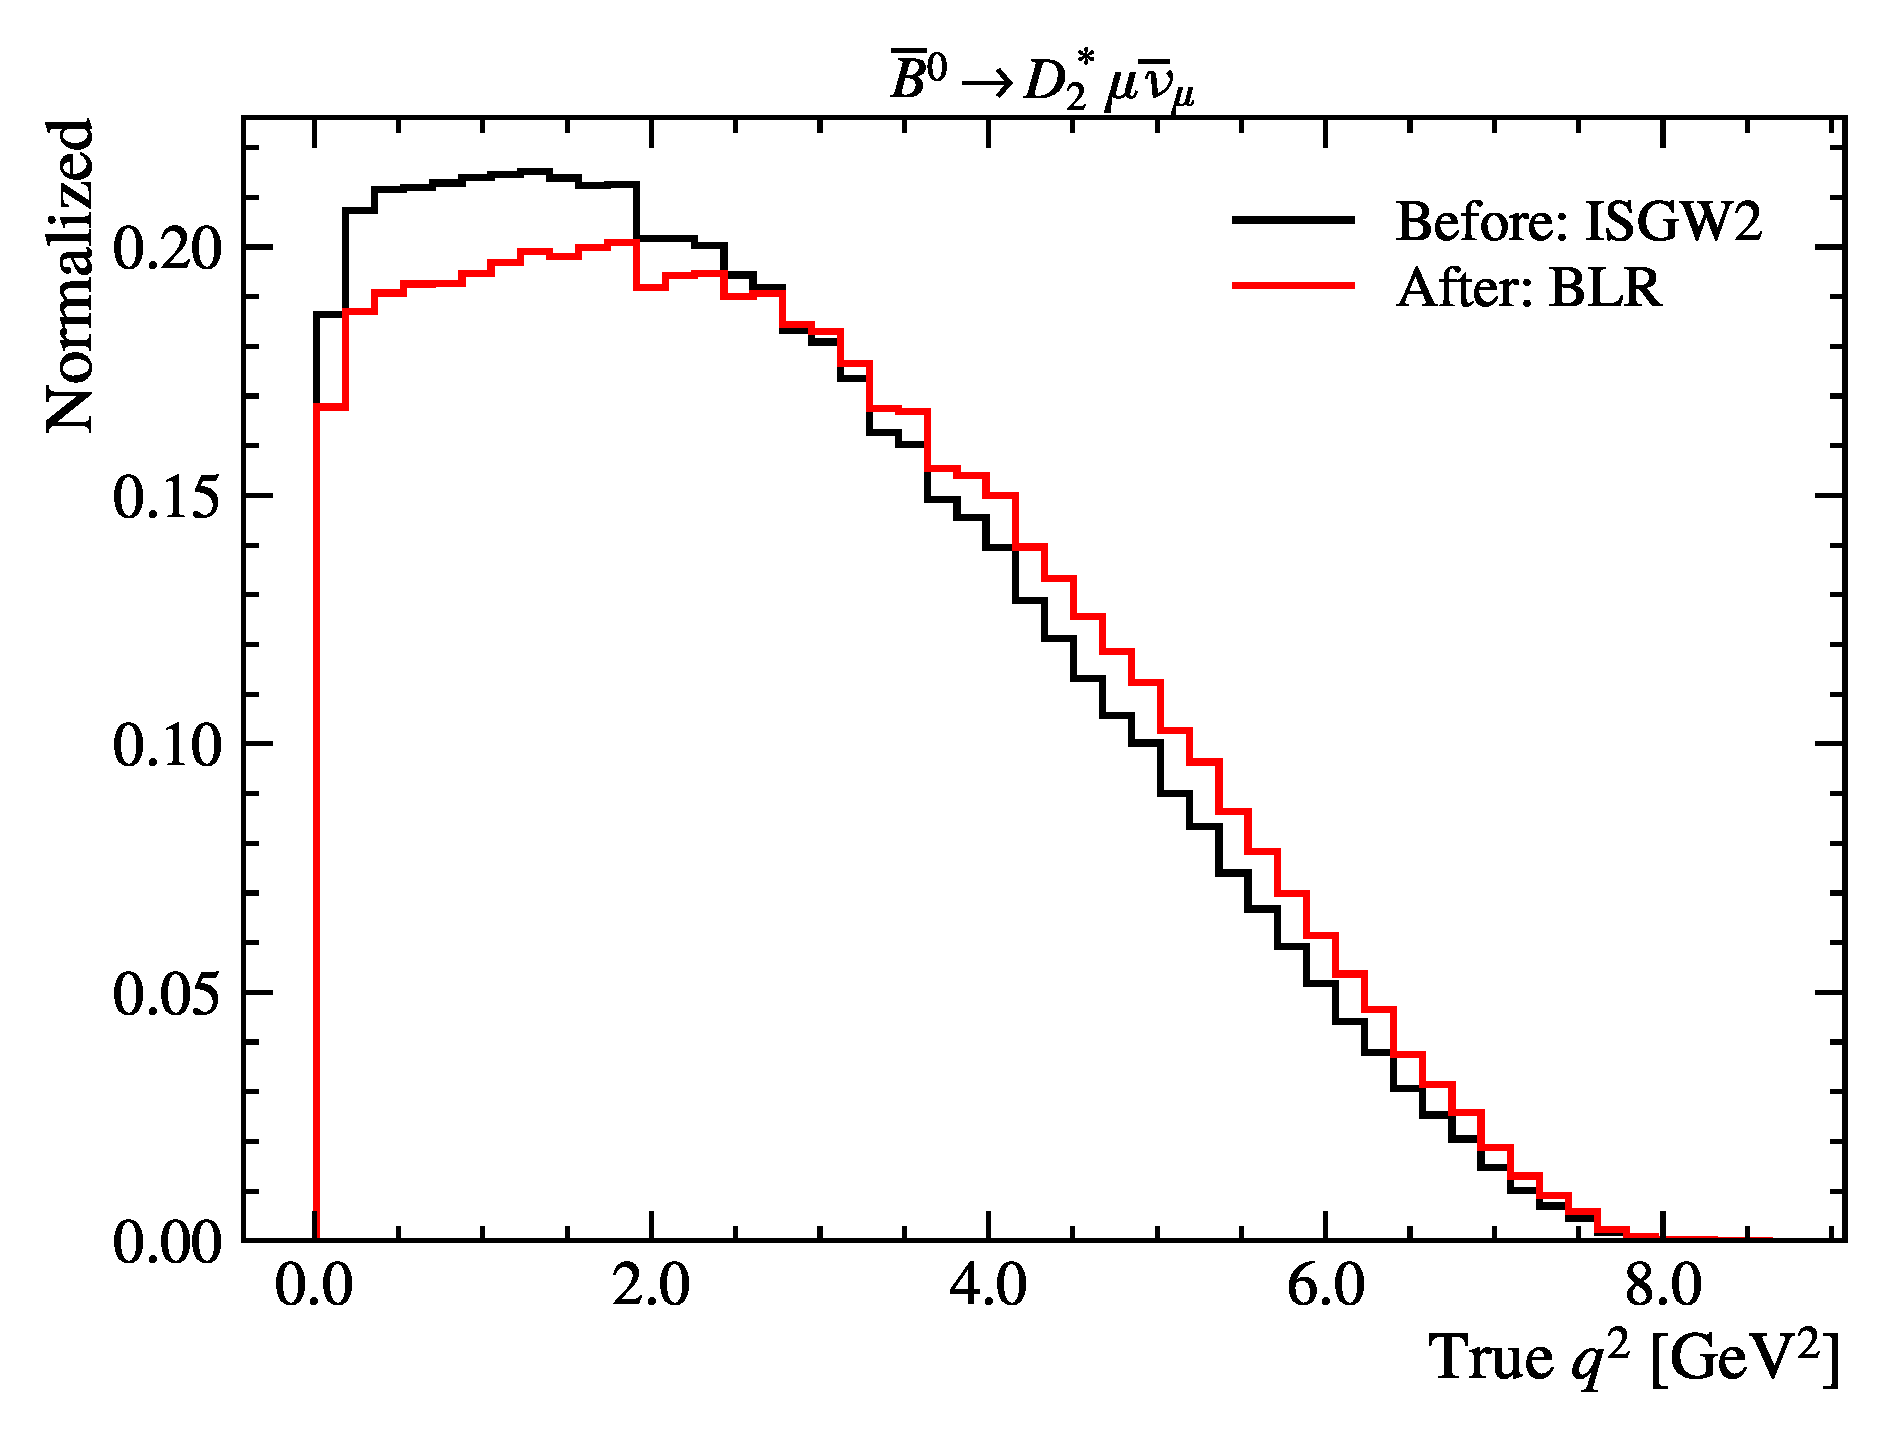
\includegraphics[width=0.24\textwidth]{
        ./figs-mc-correction/reweighting-form-factors/DststMu/D2ststMu.pdf
    }

    \caption{
        Form factor reweight effect on $D^{**}\mu$ MC templates.
        Parameters are shifted based an initial fit.
    }
    \label{fig:ff-rwt-Dstst-norm-like}
\end{figure}

\begin{figure}[ht]
    \centering
    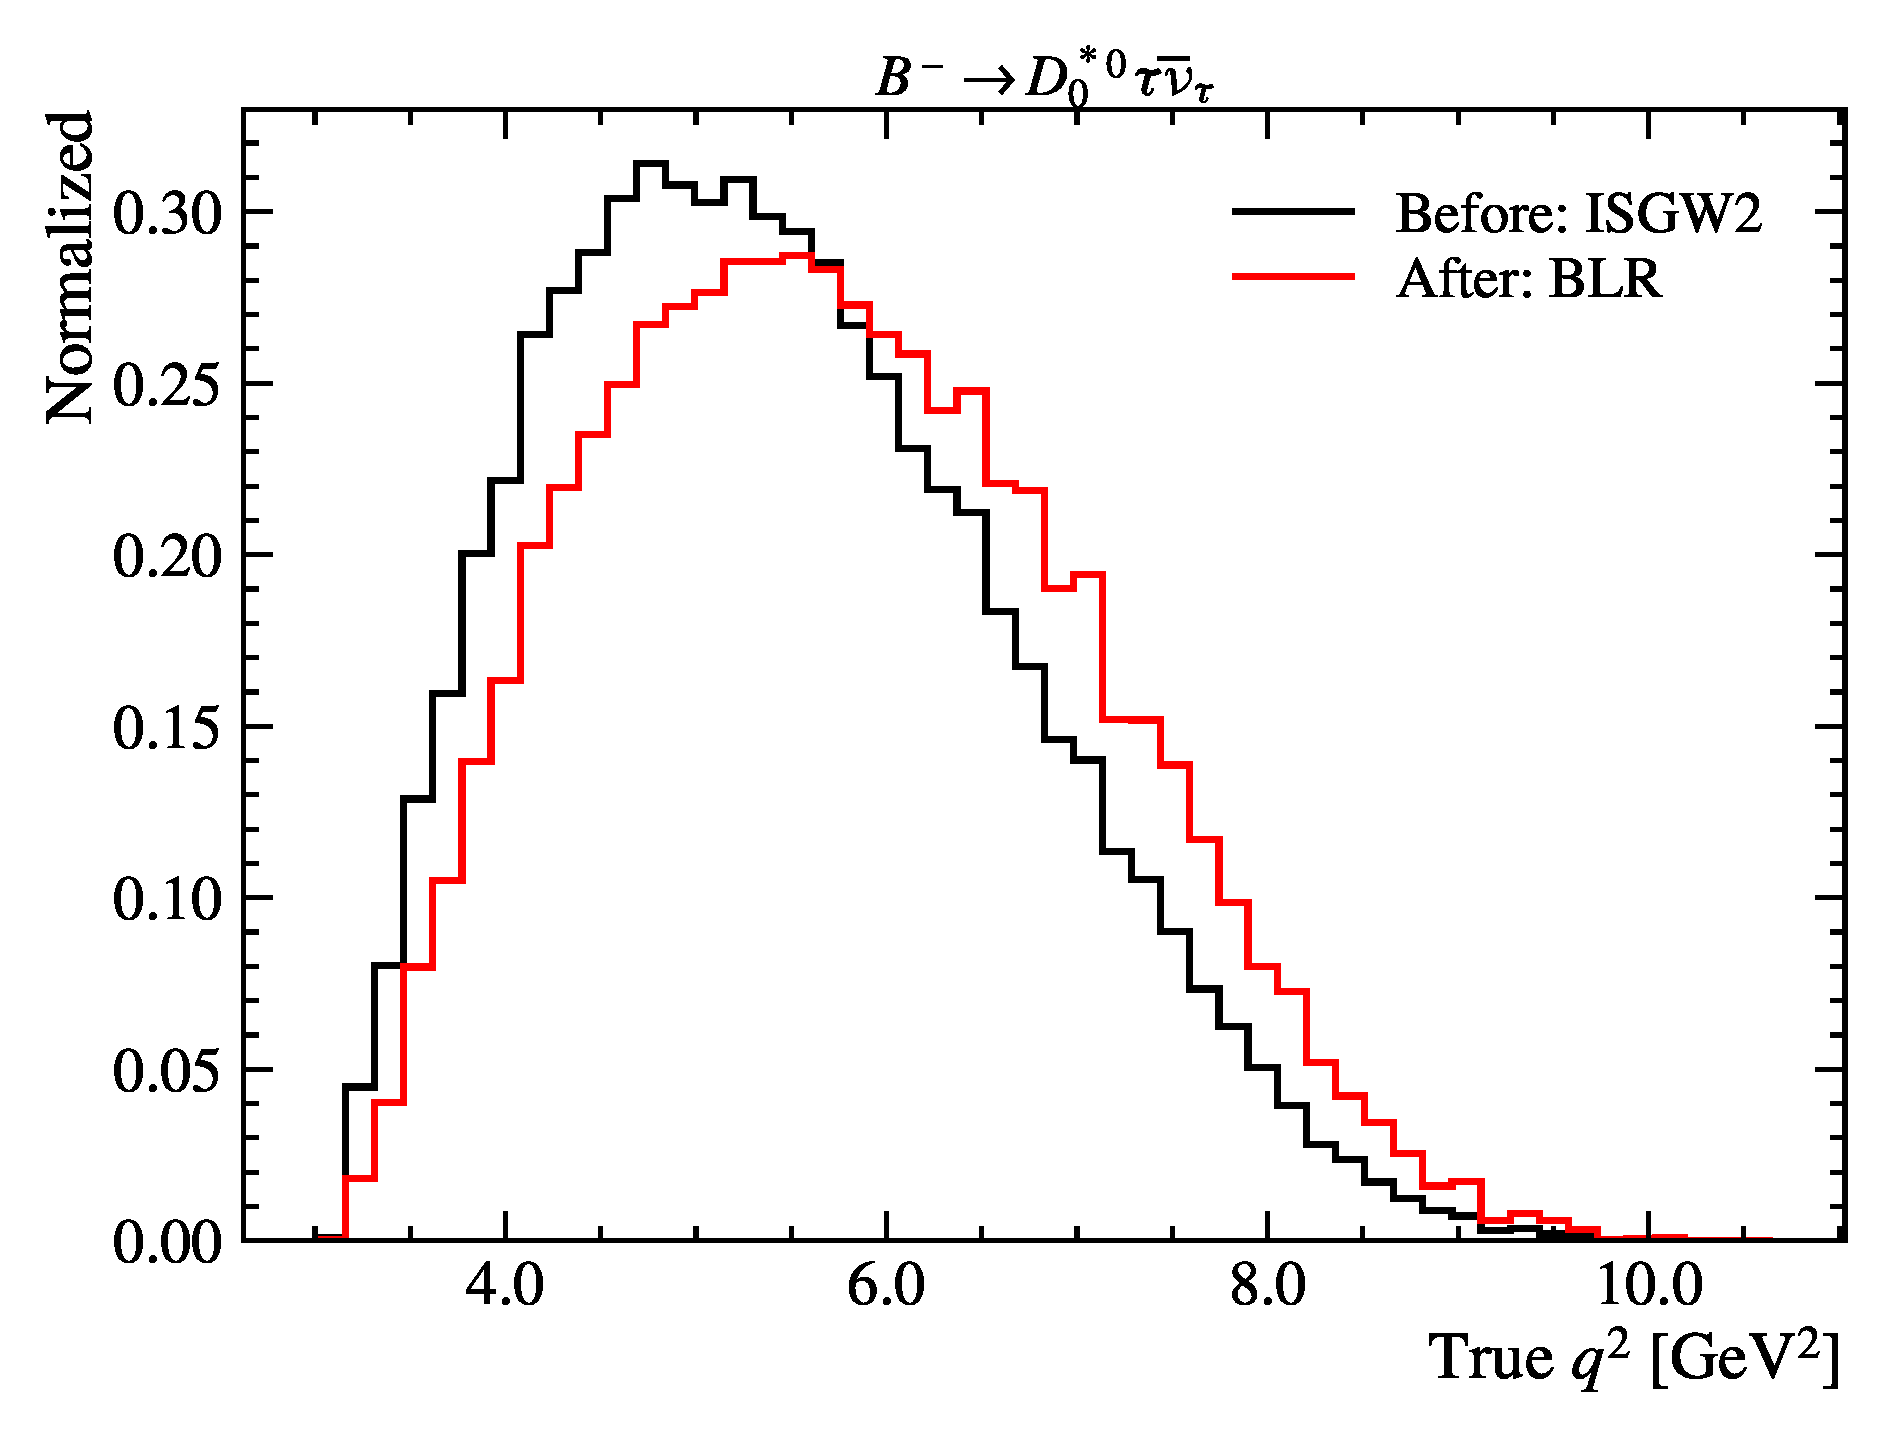
\includegraphics[width=0.24\textwidth]{
        ./figs-mc-correction/reweighting-form-factors/DststTau/D0stst0Tau.pdf
    }
    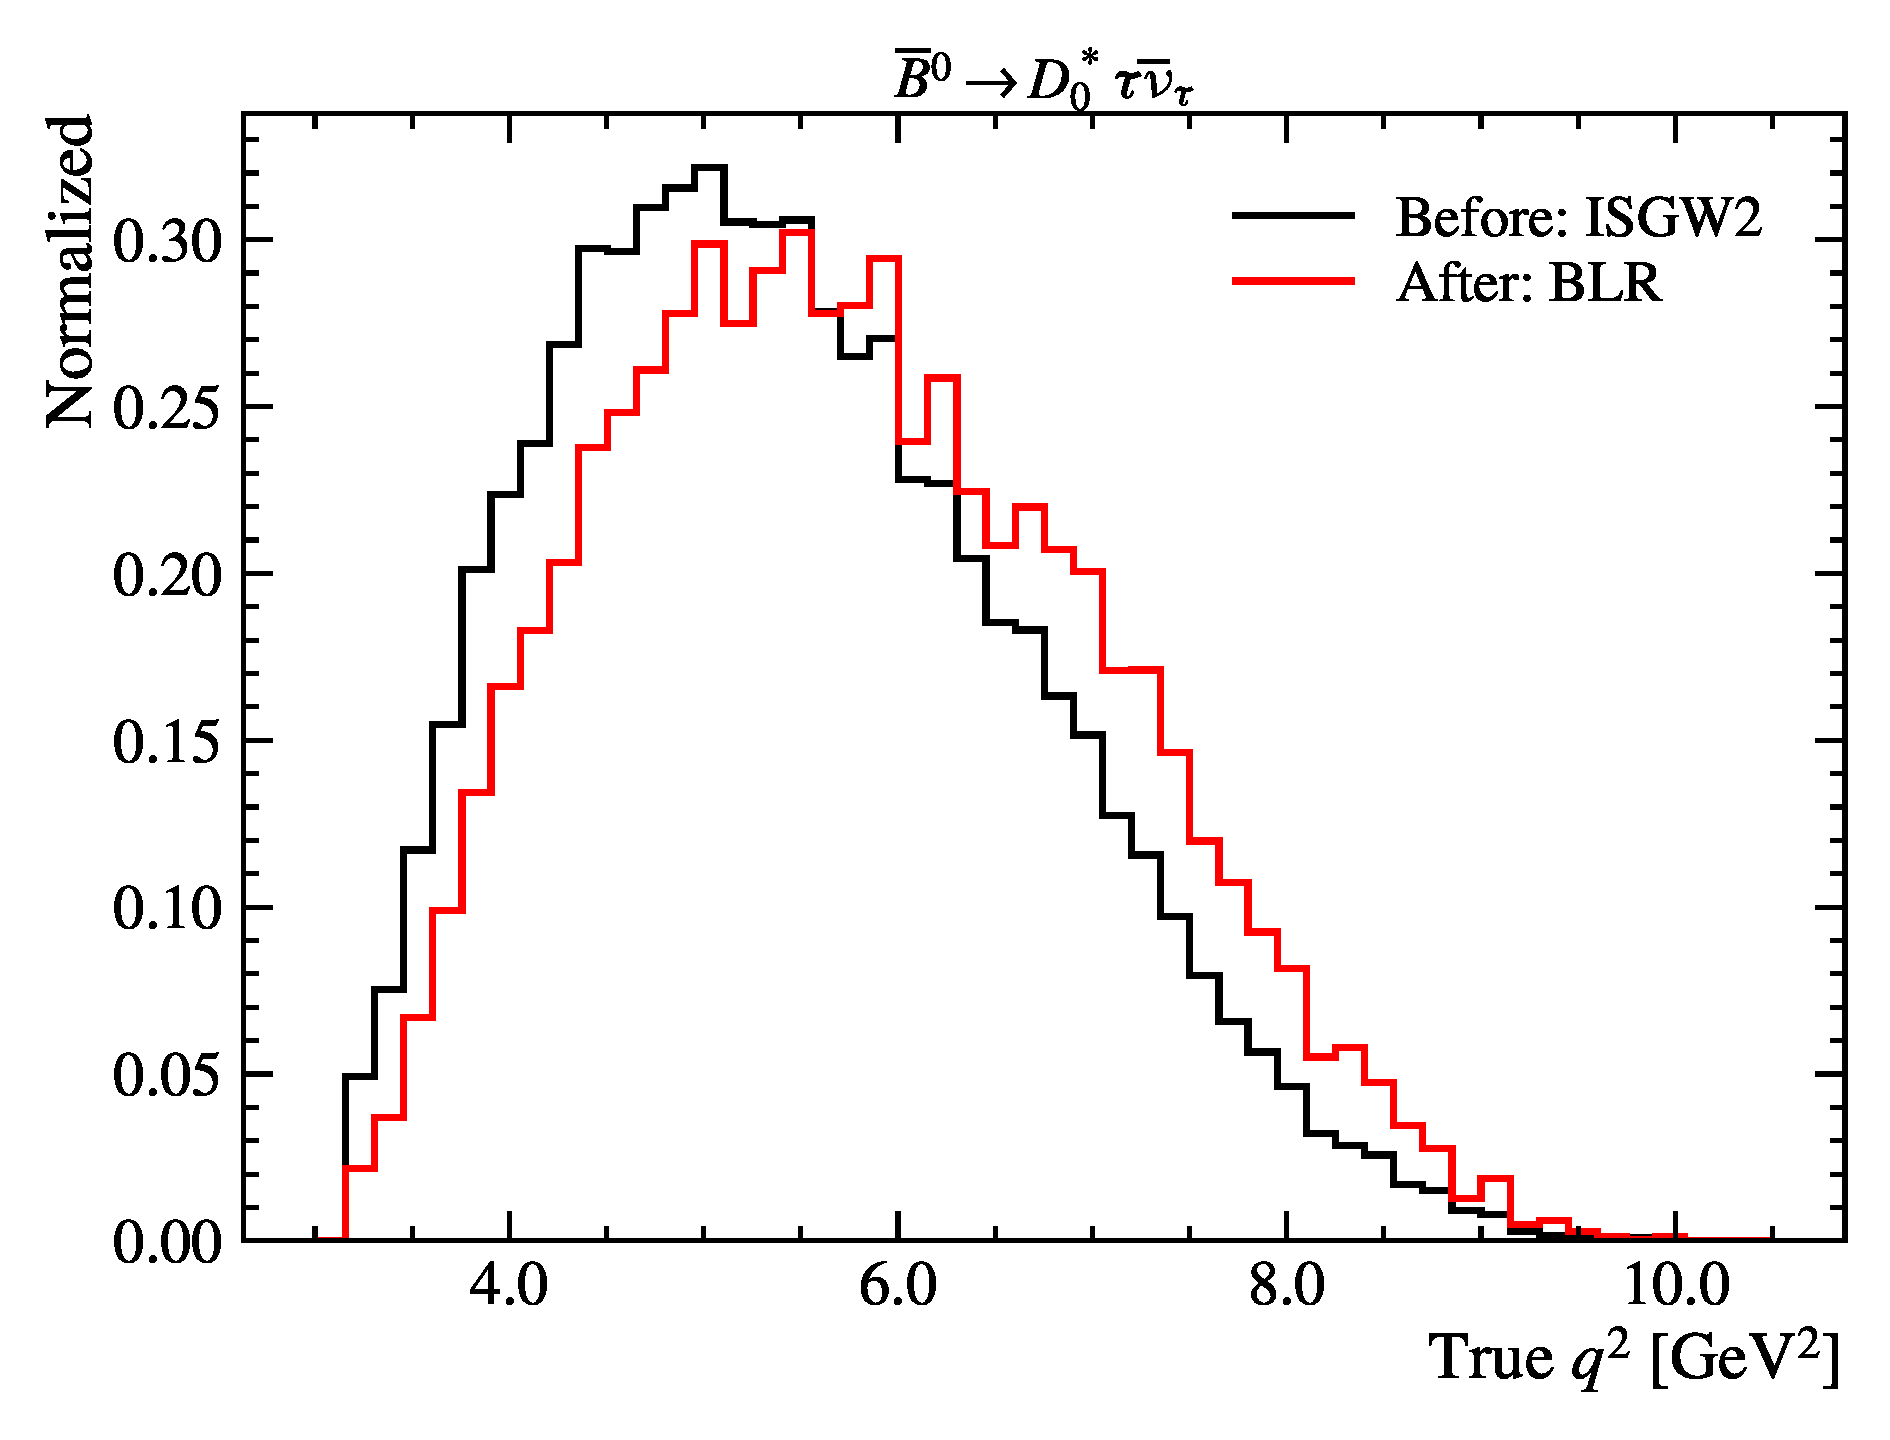
\includegraphics[width=0.24\textwidth]{
        ./figs-mc-correction/reweighting-form-factors/DststTau/D0ststTau.pdf
    }
    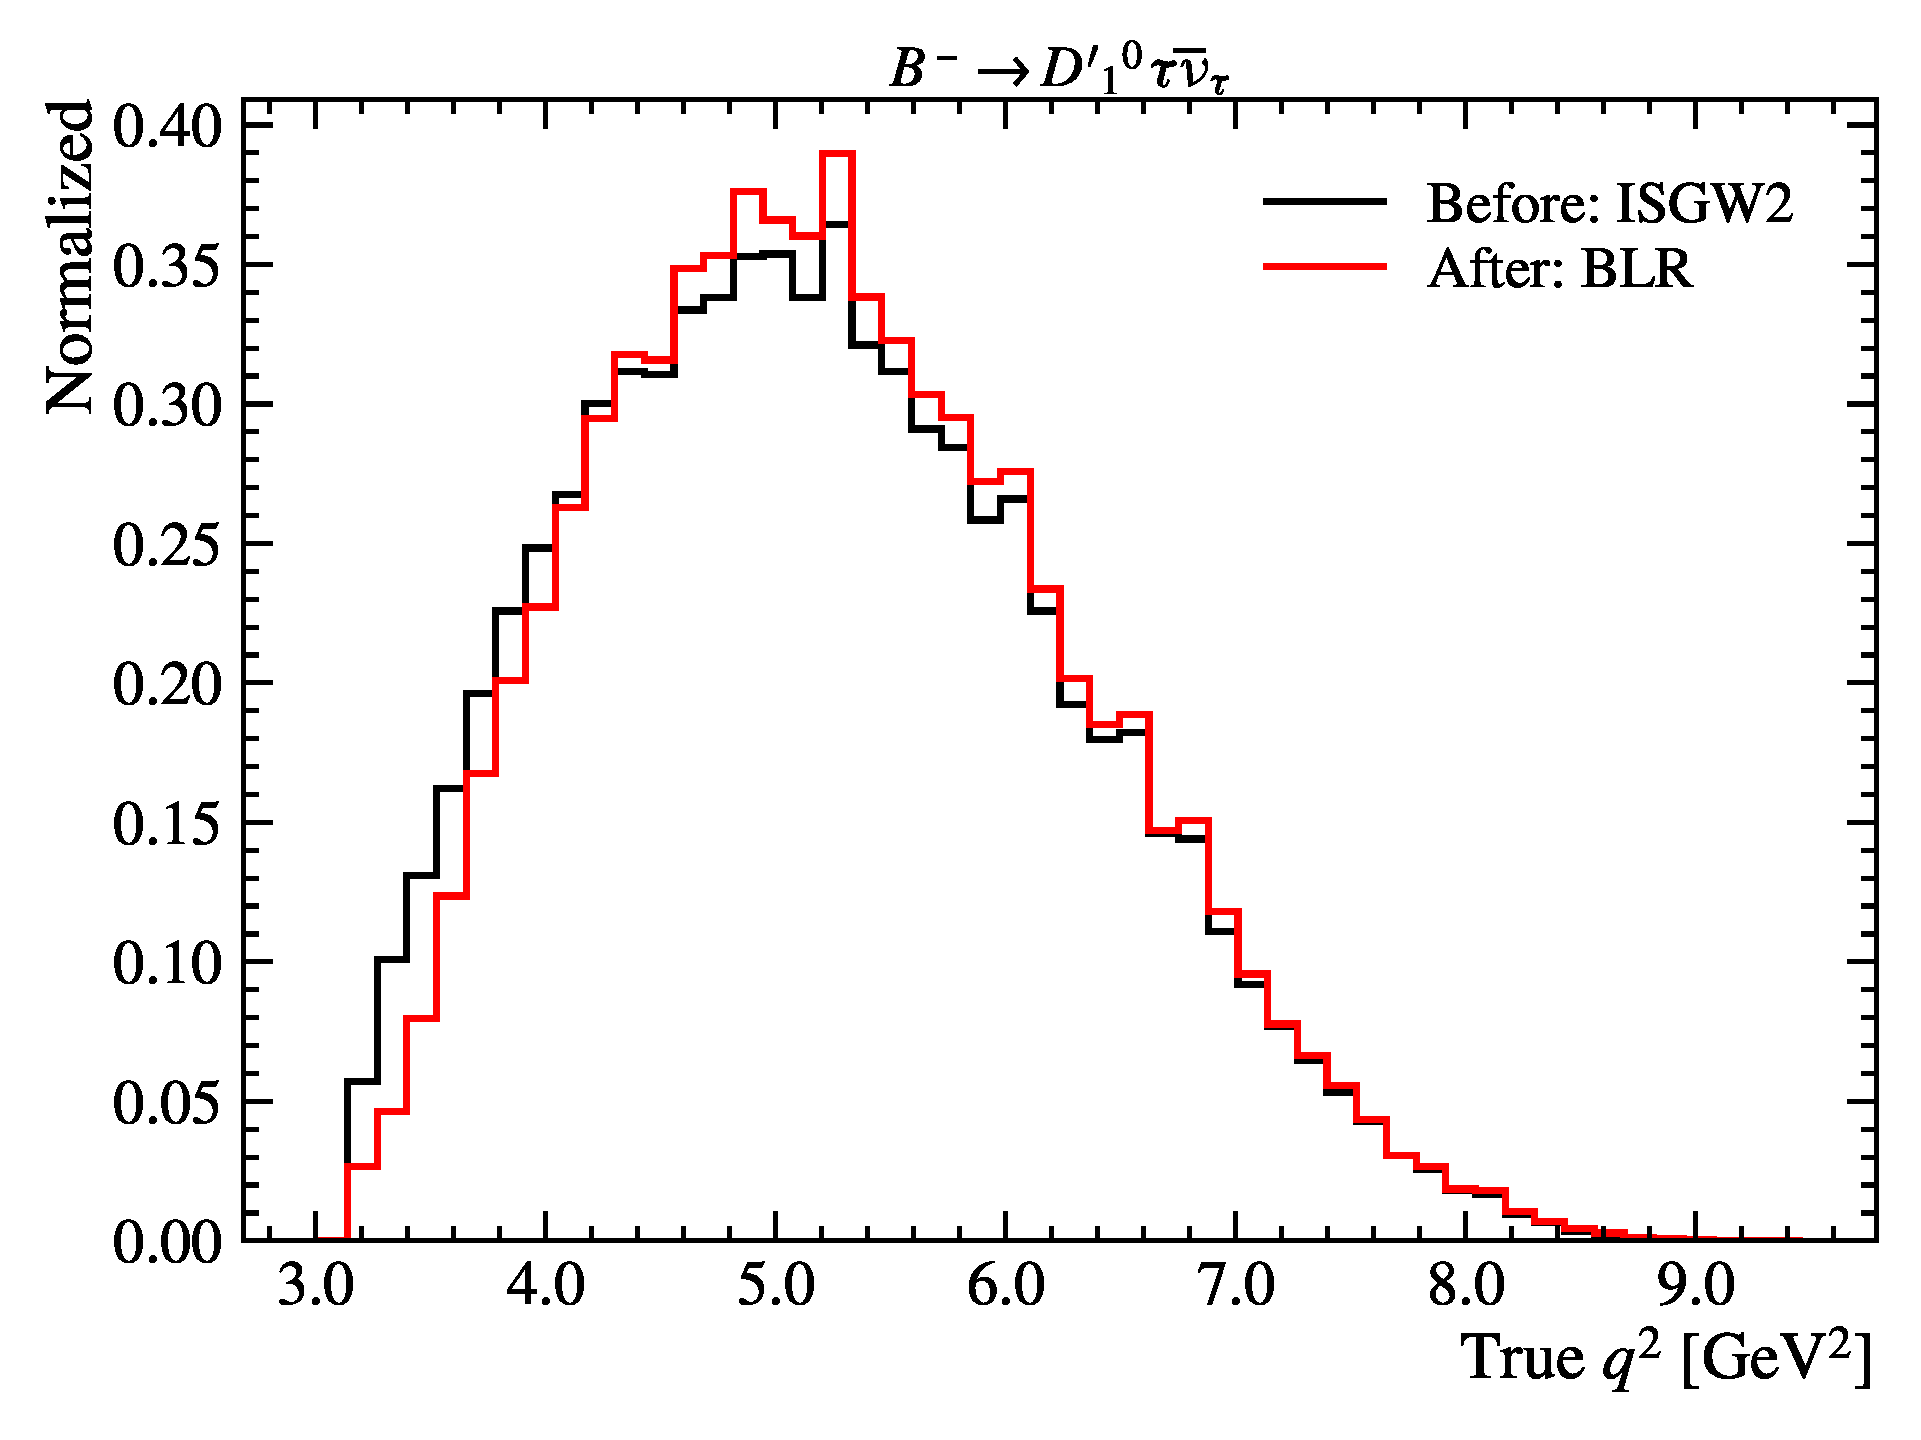
\includegraphics[width=0.24\textwidth]{
        ./figs-mc-correction/reweighting-form-factors/DststTau/D1pstst0Tau.pdf
    }
    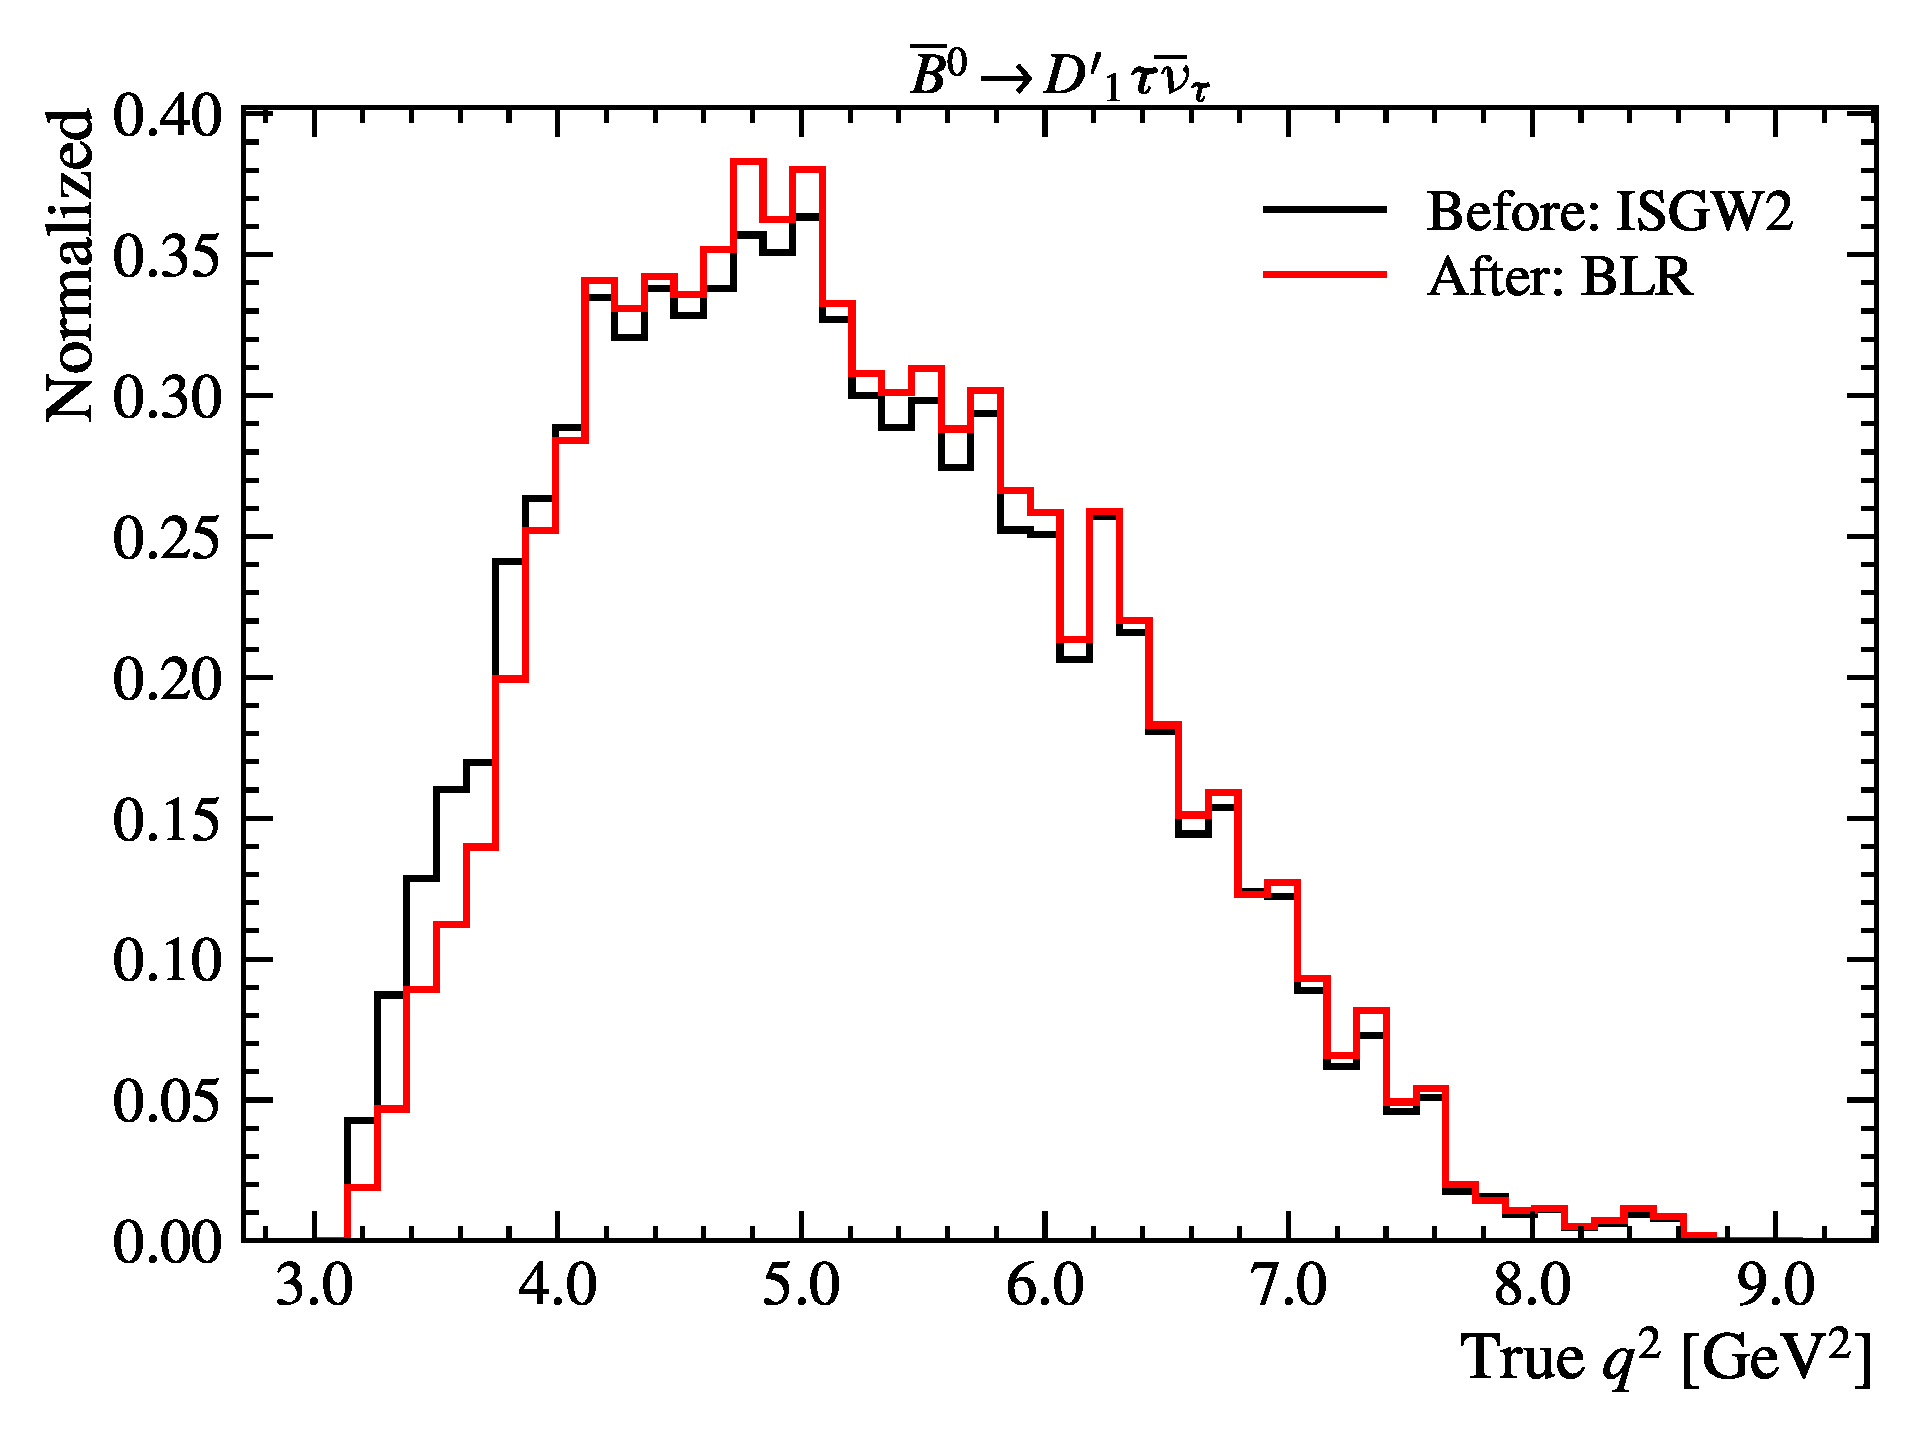
\includegraphics[width=0.24\textwidth]{
        ./figs-mc-correction/reweighting-form-factors/DststTau/D1pststTau.pdf
    }

    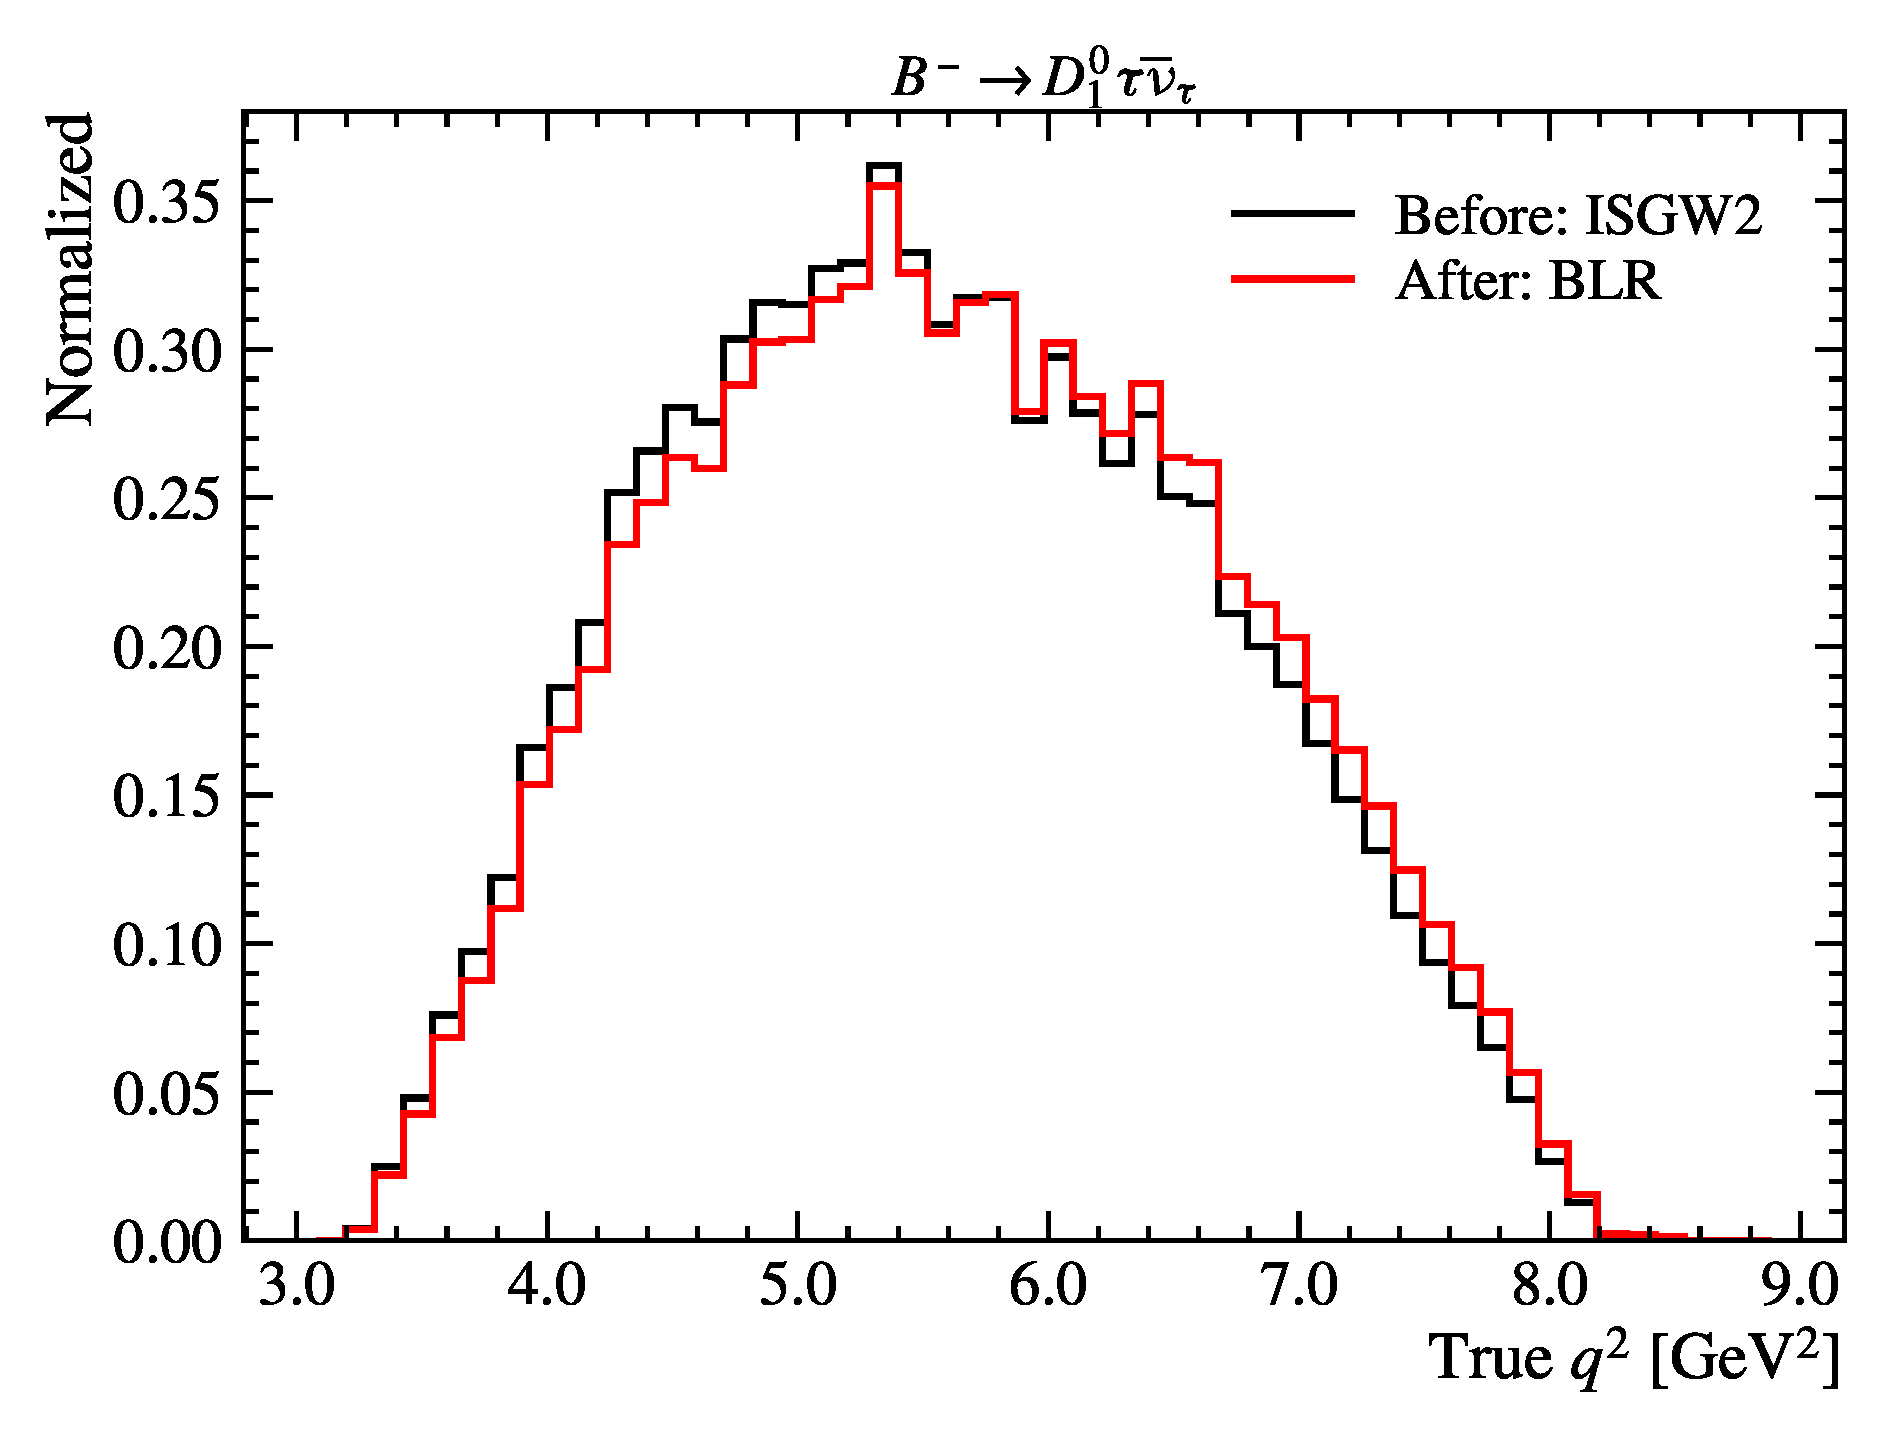
\includegraphics[width=0.24\textwidth]{
        ./figs-mc-correction/reweighting-form-factors/DststTau/D1stst0Tau.pdf
    }
    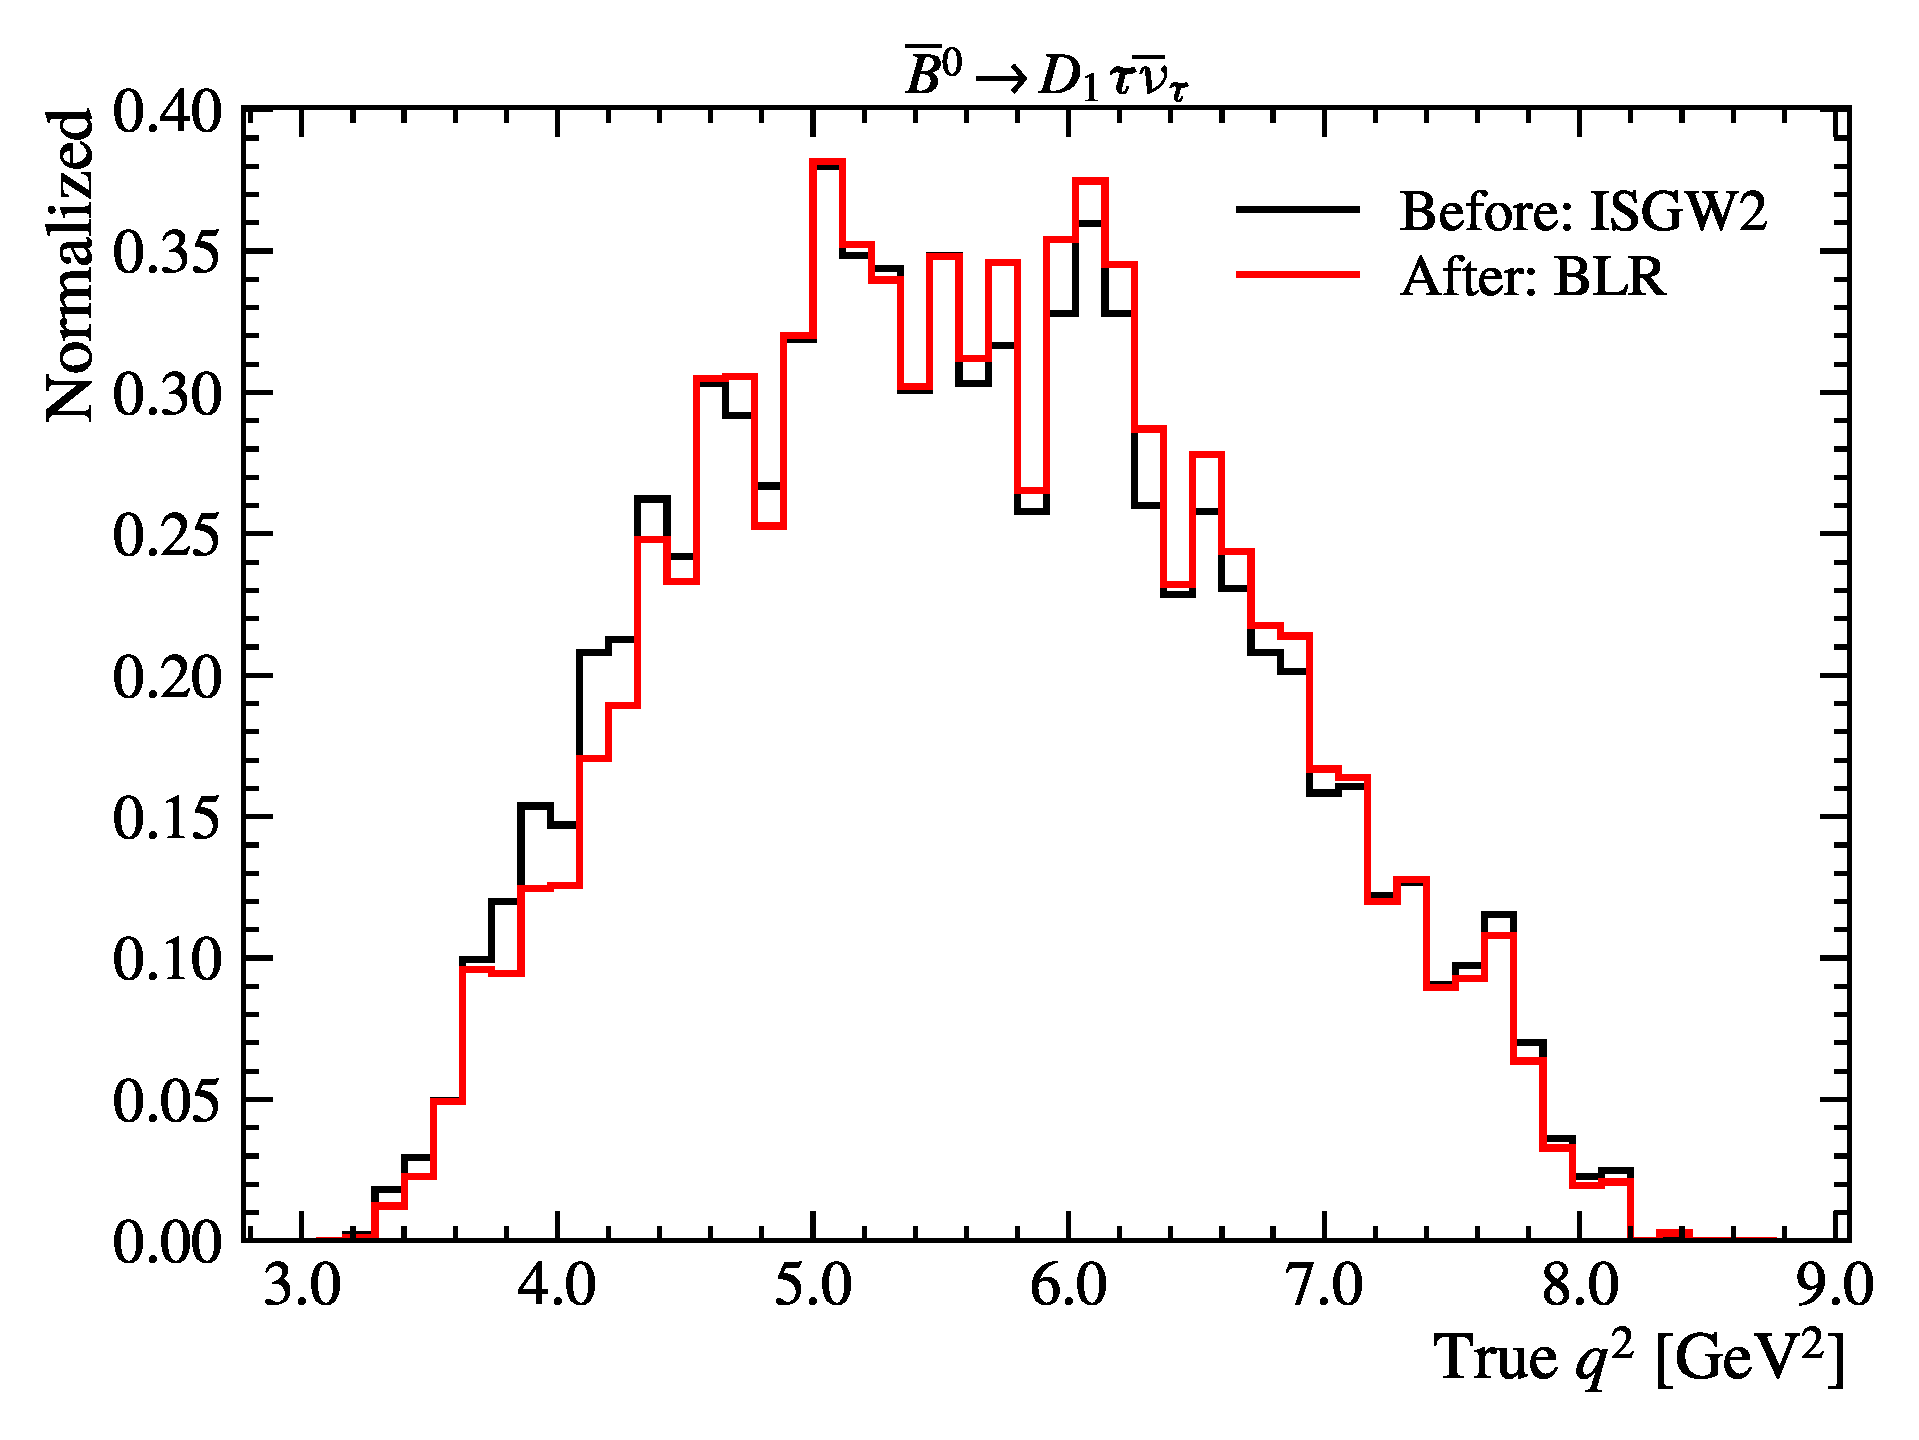
\includegraphics[width=0.24\textwidth]{
        ./figs-mc-correction/reweighting-form-factors/DststTau/D1ststTau.pdf
    }
    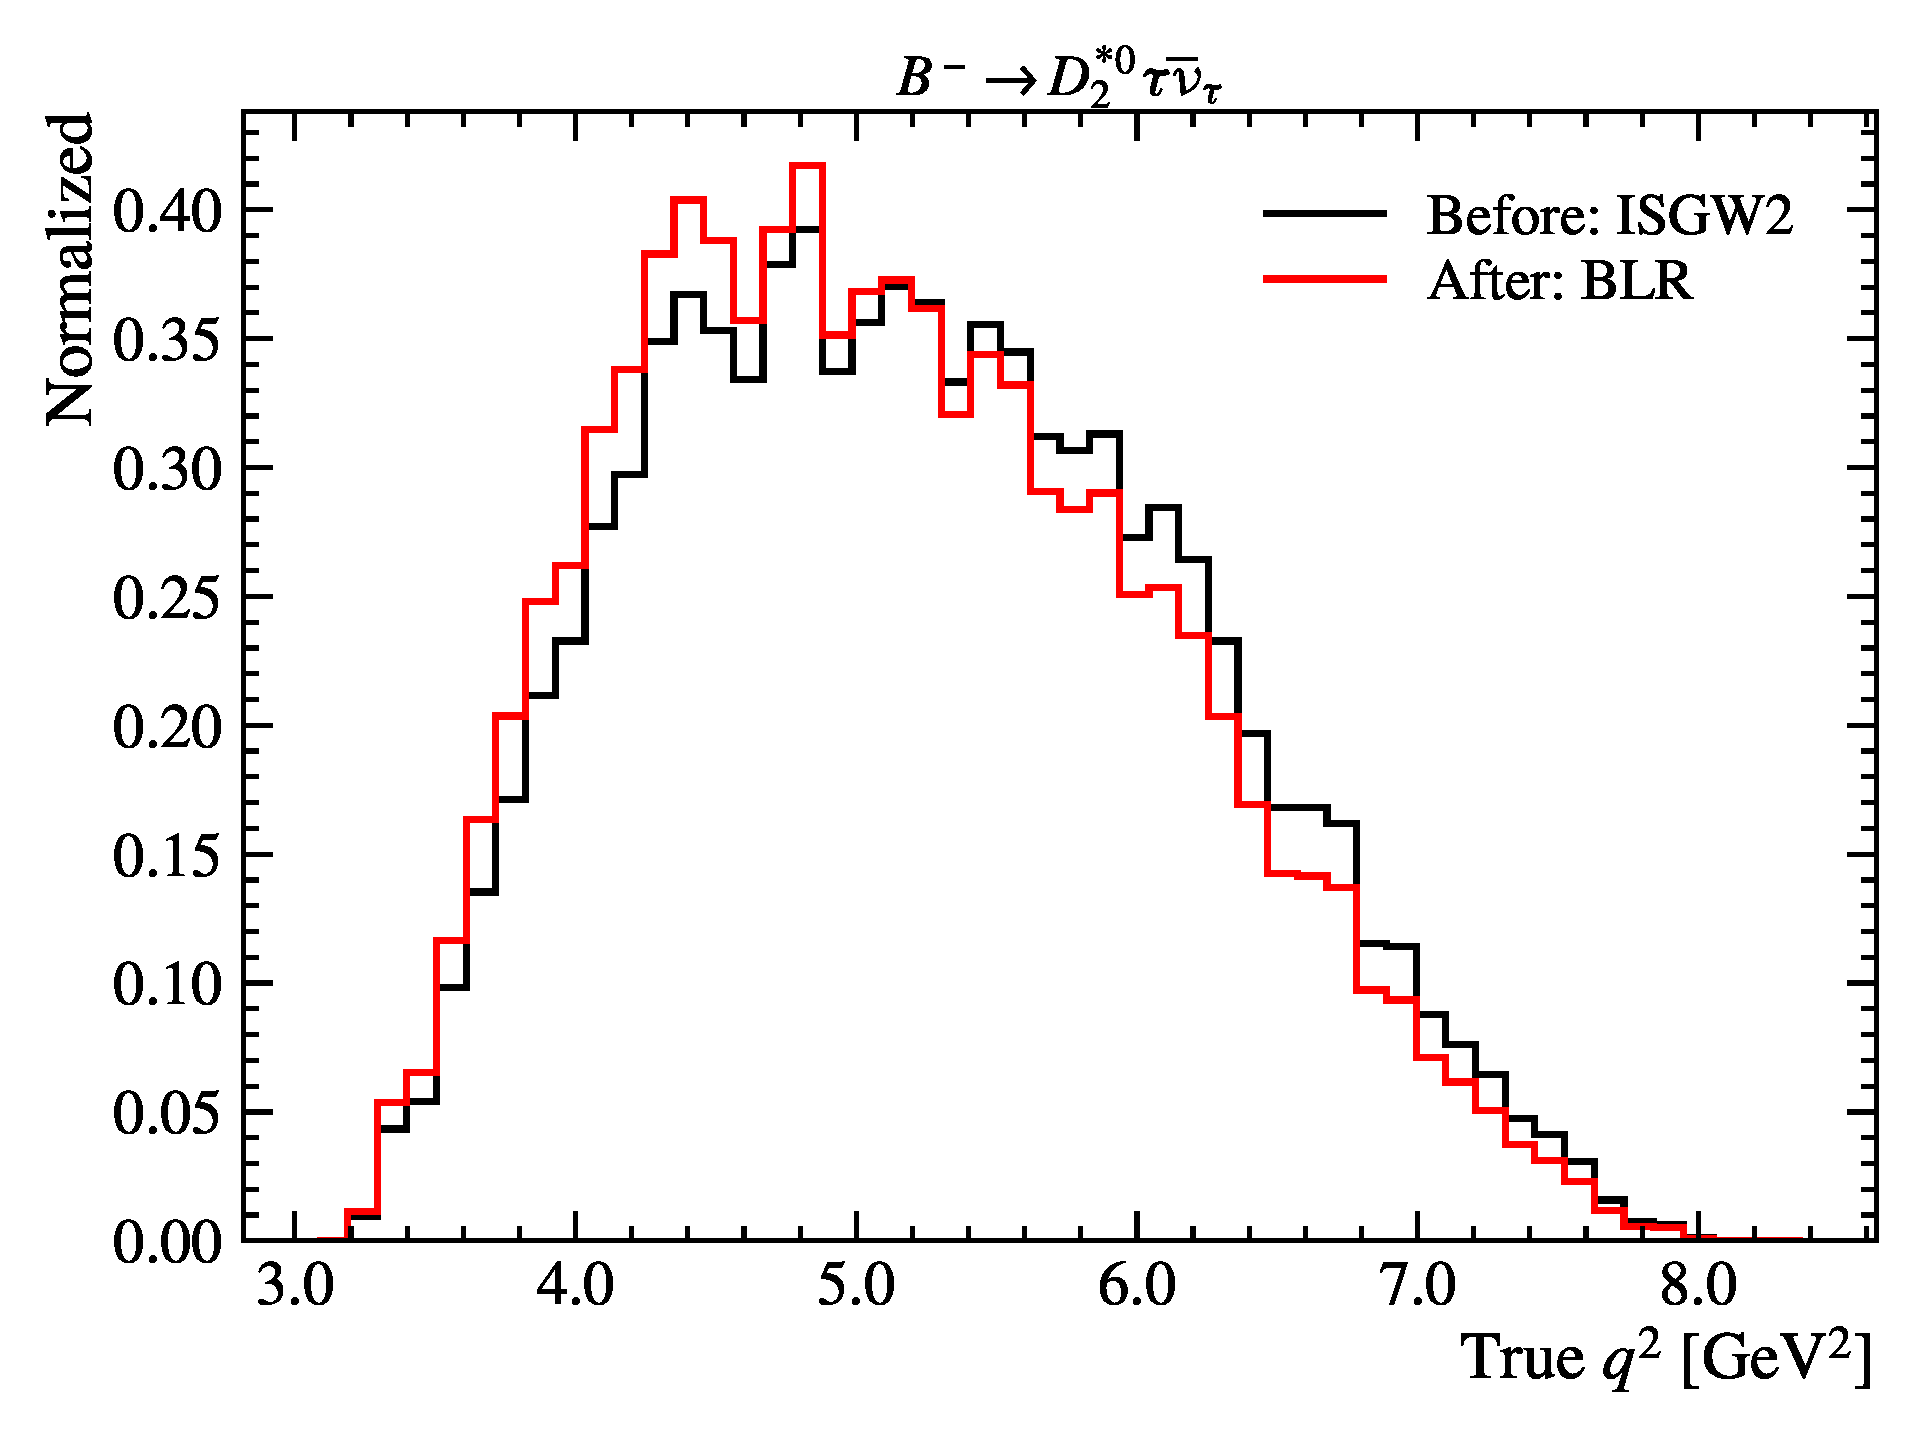
\includegraphics[width=0.24\textwidth]{
        ./figs-mc-correction/reweighting-form-factors/DststTau/D2stst0Tau.pdf
    }
    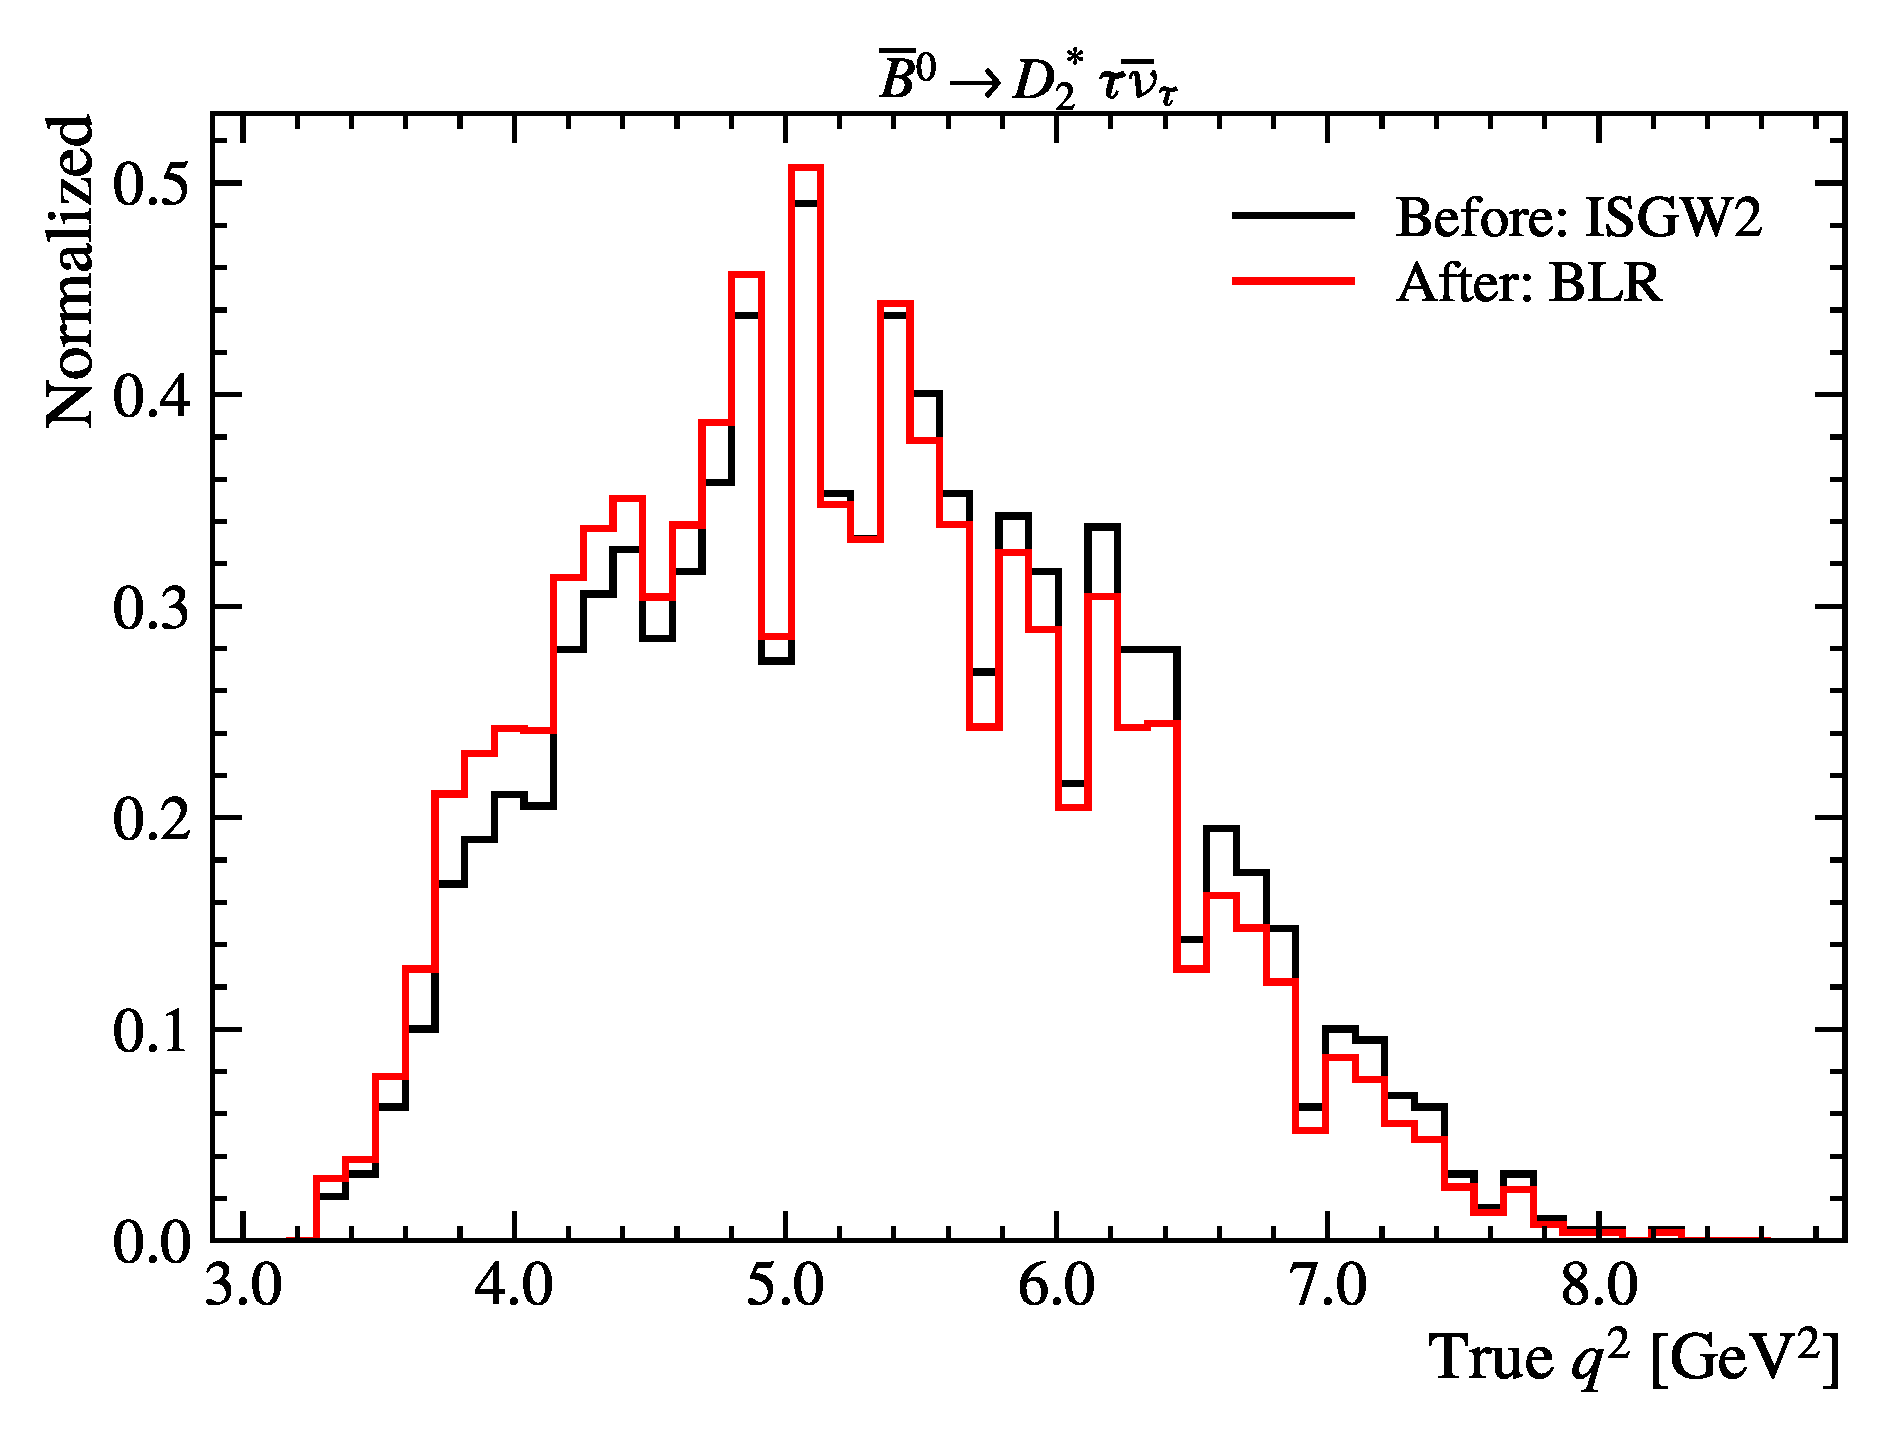
\includegraphics[width=0.24\textwidth]{
        ./figs-mc-correction/reweighting-form-factors/DststTau/D2ststTau.pdf
    }

    \caption{
        Form factor reweight effect on $D^{**}\tau$ MC templates.
        Parameters are shifted based an initial fit.
    }
    \label{fig:ff-rwt-Dstst-sig-like}
\end{figure}


\section{Initial reweighting}
\label{ref:mc-cor:init}

\subsection{Tracking efficiency}

The track reconstruction efficiencies,
defined as $\frac{N_\text{reconstructed}}{N_\text{reconstructable}}$ for
\emph{long tracks}\footnote{
    Long tracks means that the tracks have hits recorded at both VELO (upstream)
    and T-stations (downstream).
    They have the best tracking quality and most analyses use them exclusively.
},
are known to be different between data and MC.
The efficiencies are measured with a \emph{tag-and-probe} method on
$\jpsi \rightarrow \mup\mun$ samples
which involves the following steps:
First, a fully reconstructed long \muon-like track (tag) and a partially
reconstructed\footnote{
    For this analysis, partially reconstructed means that only the
    TT (tracker before the dipole magnet, to be replaced by UT)
    and T-station hits are considered for track reconstruction.
    This partially reconstructed track carries enough momentum information
    such that the invariant mass of the mother particle is reconstructed
    with high precision.

    The efficiencies computed with TT-T-station probe tracks are referred
    as \emph{long} method.
} \muon-like track (probe, which is explicitly \emph{not} a long track) is
required to form a \mun\mup vertex.
Then, the probe track is classified into two categories: The ones matched to a
long track, defined by sharing 70\% of hits with a long track in the T-stations,
and the ones \emph{not} matched to any long track.
Finally, a fit on the invariant mass of the \mun\mup vertex is performed to
extract number of signal events
separately for matched ($N_\text{sig,matched}$)
and all ($N_\text{sig,all}$) probe tracks,
and the tracking efficiency is computed as:

\begin{equation}
    \epsilon_\text{tracking} \equiv
        \frac{N_\text{reconstructed}}{N_\text{reconstructable}}
        = \frac{N_\text{sig,matched}}{N_\text{sig,all}}
\end{equation}
For more information, refer to \cite{LHCb-PUB-2011-025,LHCb-DP-2013-002}.

To correct for the tracking discrepancy between data and MC,
the efficiency ratios
($\frac{\epsilon_\text{data}}{\epsilon_\text{MC}}$),
binned in $\eta$ and \ptot of the track,
between data and MC are provided by the LHCb collaboration, which are
referred as \trackcalib efficiency ratios.
The correction is applied as a weight on a per-event basis.
The efficiency ratio table is shown in \cref{fig:trackcalib-eff}.

% Taken from RD+'s ANA
\begin{figure}[htb]
    \centering
    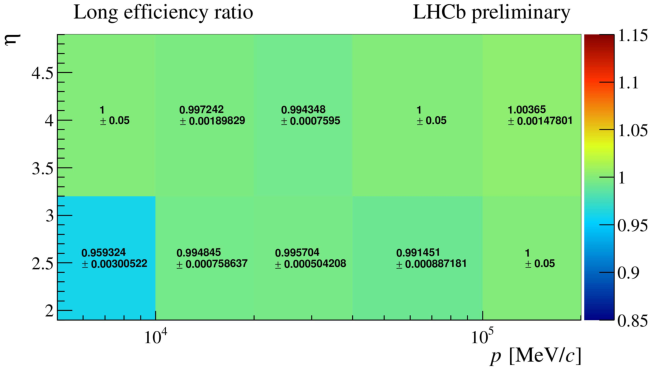
\includegraphics[width=0.6\textwidth]{./figs-mc-correction/reweighting-tracking/tracking_eff_2016.pdf}
    \caption{
        Tracking efficiency ratios
        $\frac{\epsilon_\text{data}}{\epsilon_\text{MC}}$.
        For 2016, only the table for the \emph{long} method is available.
    }
    \label{fig:trackcalib-eff}
\end{figure}

There are a few caveats: The efficiency ratios are available only for Sim09b MC
version, but in this analysis Sim09k is used.
The difference in simulation versions is ignored, given that this analysis
measures the \emph{ratio} of branching fractions, it is assumed that the
discrepancy would cancel in first order.
Additionally, the kinematic binning of \trackcalib efficiency ratios,
shown in \cref{fig:trackcalib-slow-pi}, are stricter than the signal selection
cuts in this analysis.
Most notably in slow \pion, about 50\% of the tracks falls outside of the
binning range of the table for \Dstarp\mun MC decay mode.
To circumvent the problem, one method is to apply \trackcalib binning range cuts
on both data and MC, which leads to a significant loss in selection efficiency.
It is decided that in case a track falls outside of the binning range, the
efficiency ratio from its closest bin is applied.
It is hoped that additional discrepancy will be corrected in the
\emph{final reweighting} procedure.

% Generated in lhcb-ntuples-gen/studies/plot-RDX_spi_tracking_eff:
%   ./plot_spi_tracking.py
\begin{figure}[htb]
    \centering
    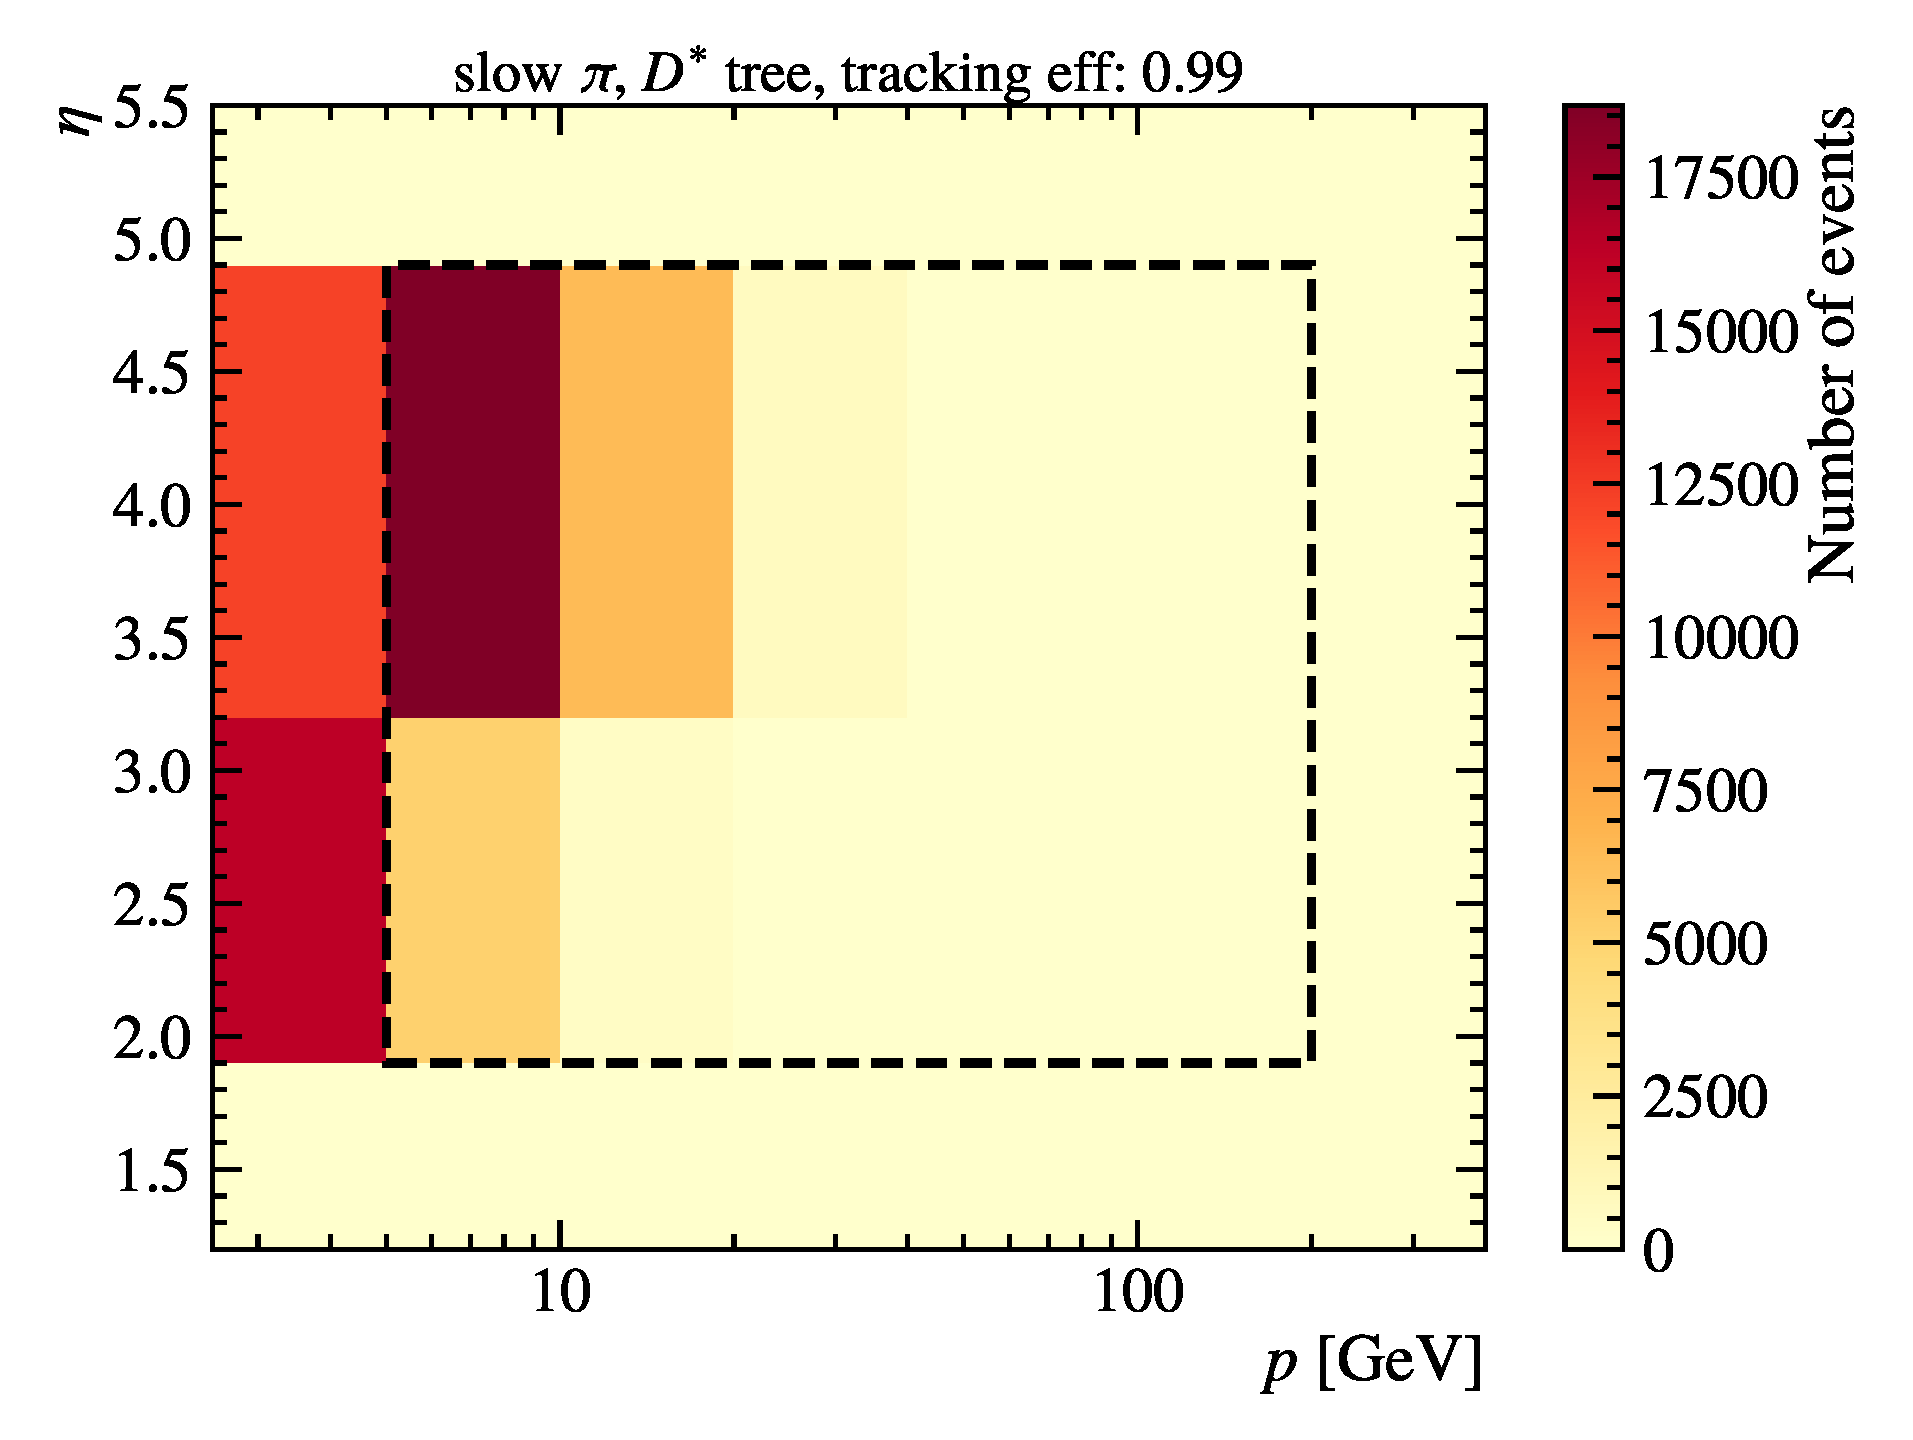
\includegraphics[width=0.7\textwidth]{./figs-mc-correction/reweighting-tracking/Dst_spi_p_eta.pdf}
    \caption{
        For slow \pion, about 50\% of tracks lies outside the binning region
        of the official \trackcalib binning range which is displayed by the
        dashed black box.
        The colored rectangles show number of events fall in each
        official \trackcalib bin.
        To avoid loss in selection efficiencies,
        correction ratios from nearby bin is applied.
        The study is done on $\Bzb \rightarrow \Dstarp \mun \neumb$ MC sample.
    }
    \label{fig:trackcalib-slow-pi}
\end{figure}


\subsection{$B$ kinematics and multiplicity}
\label{ref:mc-cor:init:jpsi-k}

Another known source of inconsistency between data and MC is the \B production
kinematics and multiplicity.
This is corrected by a separate set of
$\Bp \rightarrow \jpsi (\rightarrow \mun\mup) \Kp$
control samples, selected by a procedure described
in \cref{ref:sel:aux}.
Additionally, the track efficiency correction described in the previous section
is applied on the \jpsi\kaon MC sample.

To separate \jpsi\kaon signal from combinatorial background,
A fit, shown in \cref{fig:fit-JpsiK-data},
is performed on invariant mass of the $B$ meson ($m_B$) of \jpsi\kaon data.
The fit model consists of a double Gaussian plus a Crystal bell for
signal, and an exponential background.
A \sPlot\ procedure,
a fit-based approach to subtract background as described in
\cite{Pivk_2005},
then computes signal and background weight for each event.
Distributions of variables uncorrelated with $m_B$, for example \pt of $B$,
are produced by applying signal weights (\sWeight) obtained above on all
data events.

% Generated in /lhcb-ntuples-gen/run2-JpsiK, with:
%   make fit-2016
% need to install zfit, which can be done via:
%   pip install -r ./requirements.txt
% in the same folder. And for now this probably doesn't work on macOS
\begin{figure}[htb]
    \centering
    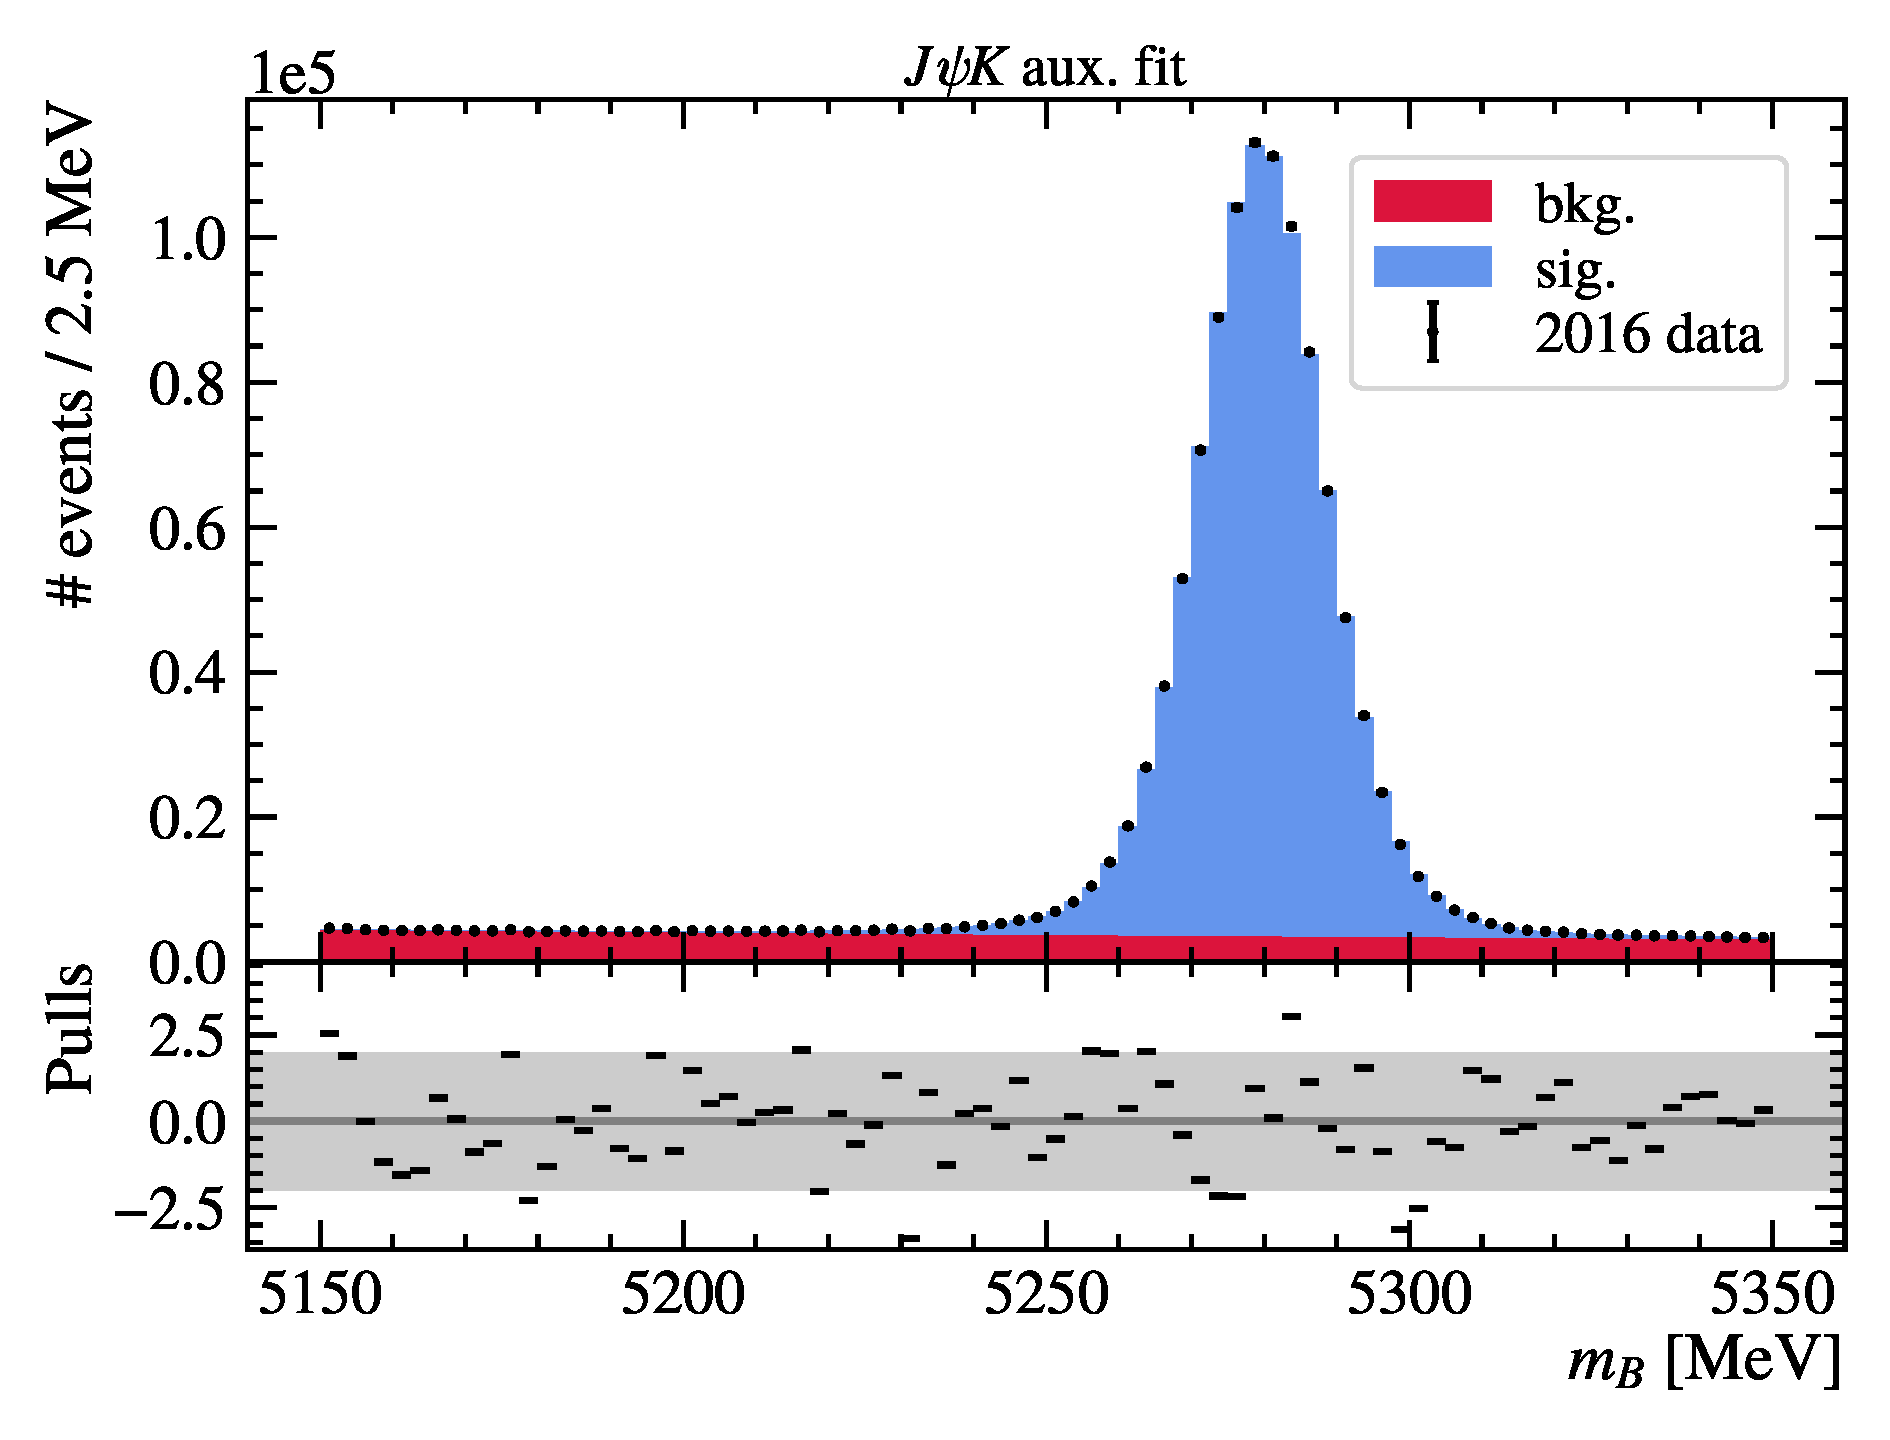
\includegraphics[width=0.45\textwidth]{./figs-mc-correction/reweighting-JpsiK/fit-JpsiK/fit_final.pdf}
    \hspace{1em}
    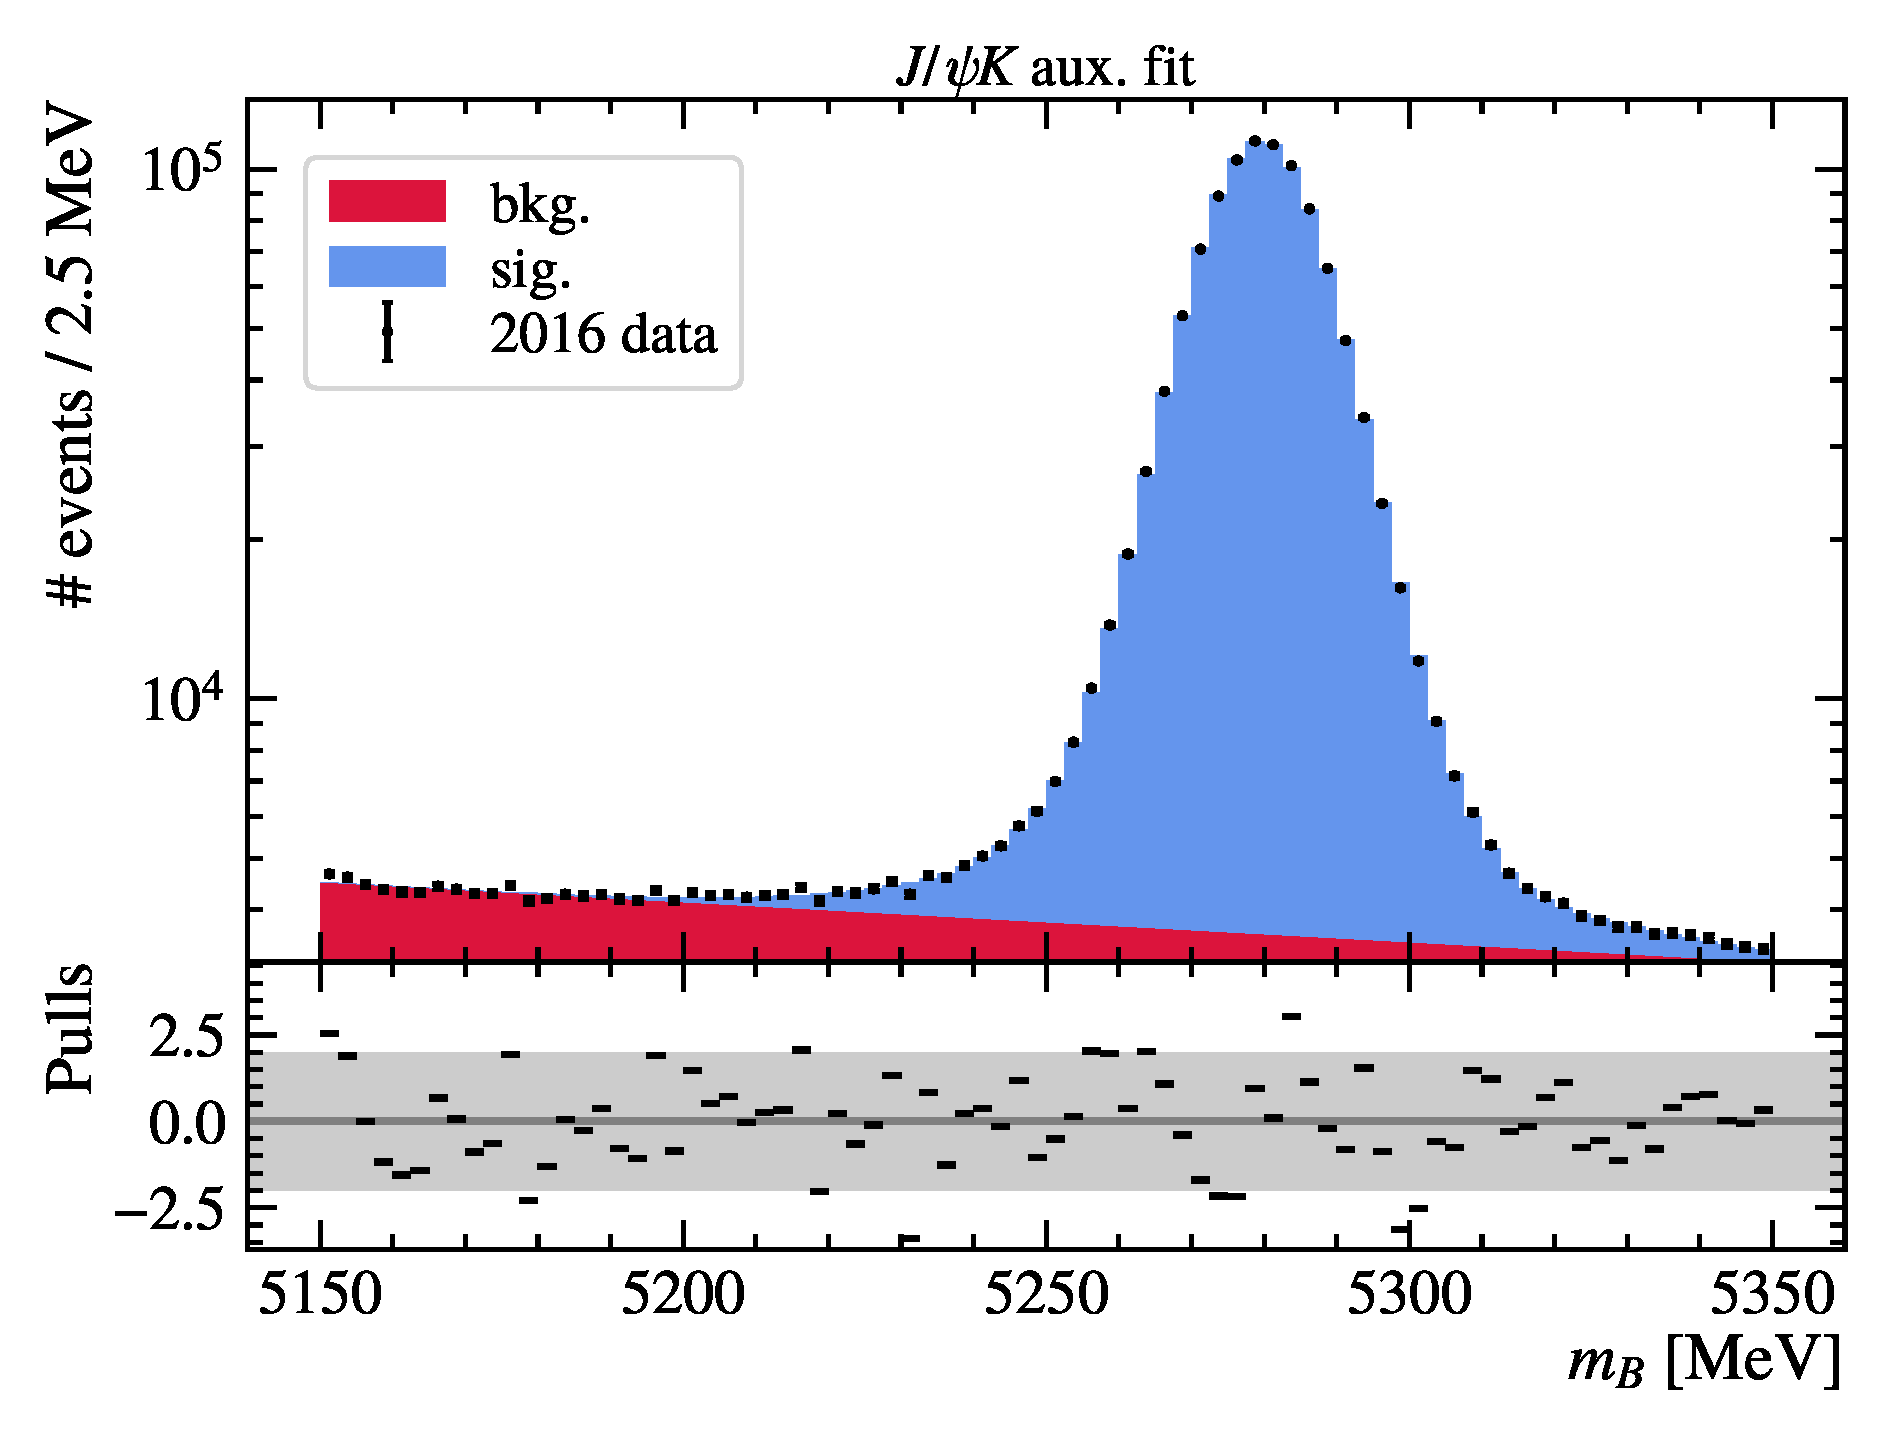
\includegraphics[width=0.45\textwidth]{./figs-mc-correction/reweighting-JpsiK/fit-JpsiK/fit_final_log_scale.pdf}

    \caption{
        Fit on $J/\psi K$ with a \sPlot procedure.
        The signal is modelled by a double Gaussian plus a Crystal bell;
        the background an exponential.
        Left and right show the same plot, with left having a linear $y$ axis,
        and right a log $y$ axis.
    }
    \label{fig:fit-JpsiK-data}
\end{figure}

A multi-stage\footnote{
    ``Multi-stage'' means that for reweighting stage $i$,
    all previous $i-1$ weights are applied.
} reweighting is performed on \sWeight-ed data and MC
(both are normalized, so the reweighting only corrects shape differences),
with stages defined in \cref{tab:rwt-JpsiK},
and the results shown in \cref{fig:rwt-JpsiK}.
The occupancy (nTracks) has to be corrected first before $B$ kinematics,
because the PID efficiency weights depend on nTracks, and the PID weights alter
the shapes of the kinematic distributions of the \B decay daughters, which in
turn affect the \B kinematic distributions themselves.
The reweighting binning ranges are chosen such that:
\begin{itemize}
    \item They cover most of signal ranges of the data after applying \sWeight.
    \item The MC have enough population within these binning
        ranges so that there is no or few bins without a event.
\end{itemize}

When applying the \jpsi\kaon-derived weights to the nominal MC sample,
for events outside the binning regions,
the weights from nearby bins are applied.
This is to avoid introducing explicit kinematic cuts on the \B meson,
which is hard to apply consistently due to the fact that for
$B \rightarrow \jpsi\kaon$ decays,
there is no missing particle in the decay chain thus the \B momentum is
reconstructed in a more complete way,
whereas for $B \rightarrow D^{(*)} \lepton\neulb$, the missing neutrino(s)
makes the reconstructed \B momentum incomplete.

\begin{table}[htb]
    \centering
    \caption{
        Reweighting stages and binning schemes for \B kinematic and
        occupancy reweighting.
    }
    \label{tab:rwt-JpsiK}
    \begin{tabular}{ c | c | c | c | c }
        \toprule
        {\bf Variable 1}    & {\bf Binning 1}      & {\bf Variable 2}   & {\bf Binning 2}    & {\bf Figure}   \\
        \midrule
        \B PV ndf           & 20, 1--250           & nTracks            & 20, 0--450         & \cref{fig:rwt-JpsiK:stage1} \\
        \B $\eta$           & 9, 2--6              & \B \pt             & 20, 0--30 GeV      & \cref{fig:rwt-JpsiK:stage2} \\
        \bottomrule
    \end{tabular}
\end{table}

% Generated in /lhcb-ntuples-gen/studies/plot-JpsiK_kinematic_reweighting
% by running:
%   plot_JpsiK_reweighting.py
% in the specified folder
\begin{figure}[htb]
    \begin{subfigure}{\textwidth}
        \centering
        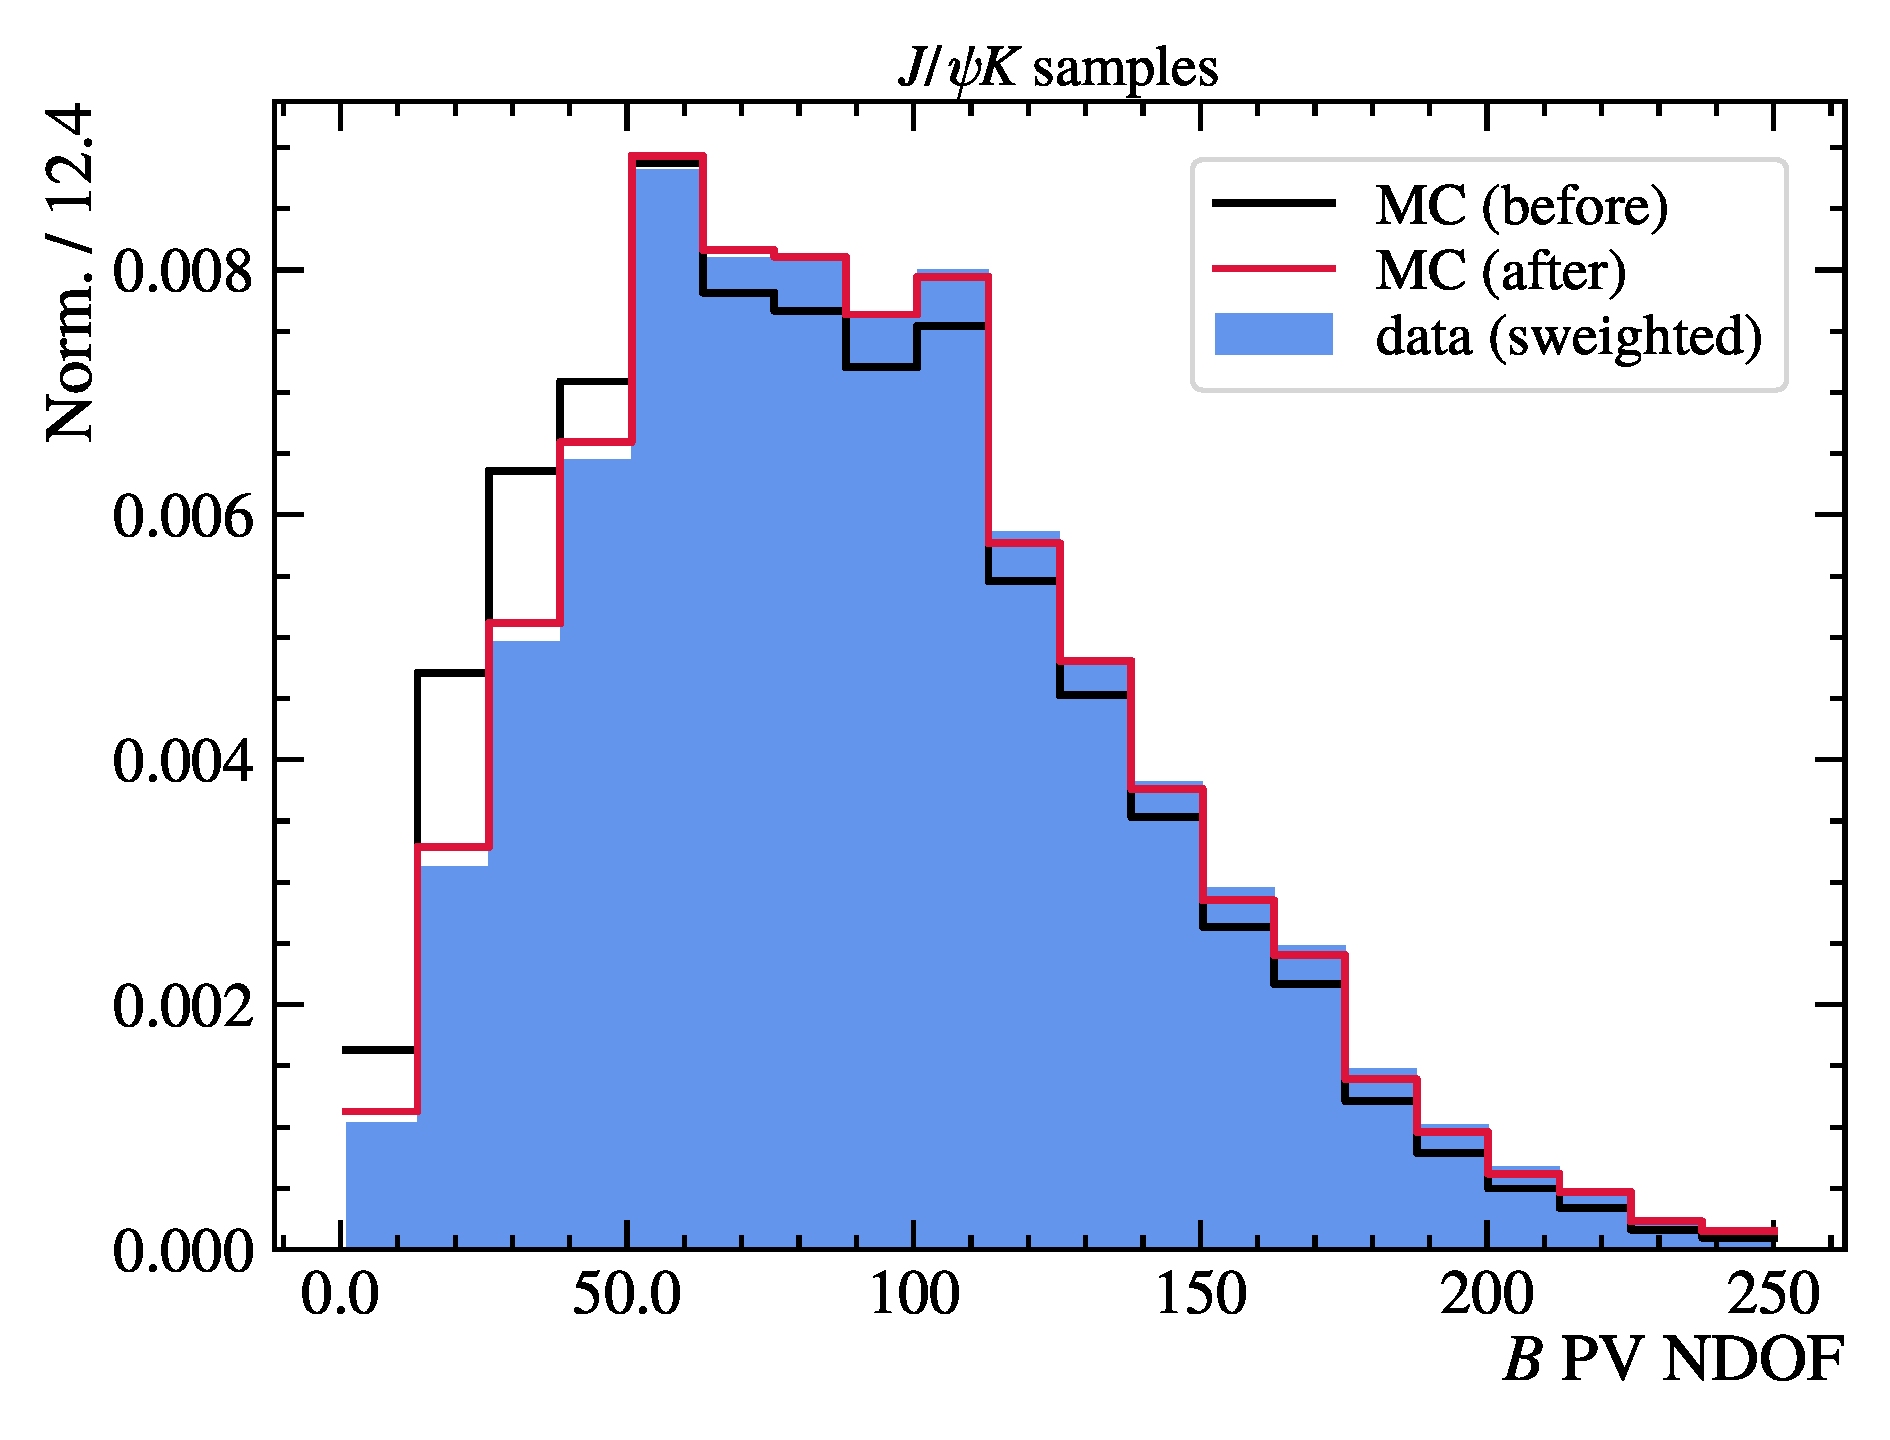
\includegraphics[width=0.45\textwidth]{./figs-mc-correction/reweighting-JpsiK/reweight-JpsiK/b_ownpv_ndof.pdf}
        \hspace{1em}
        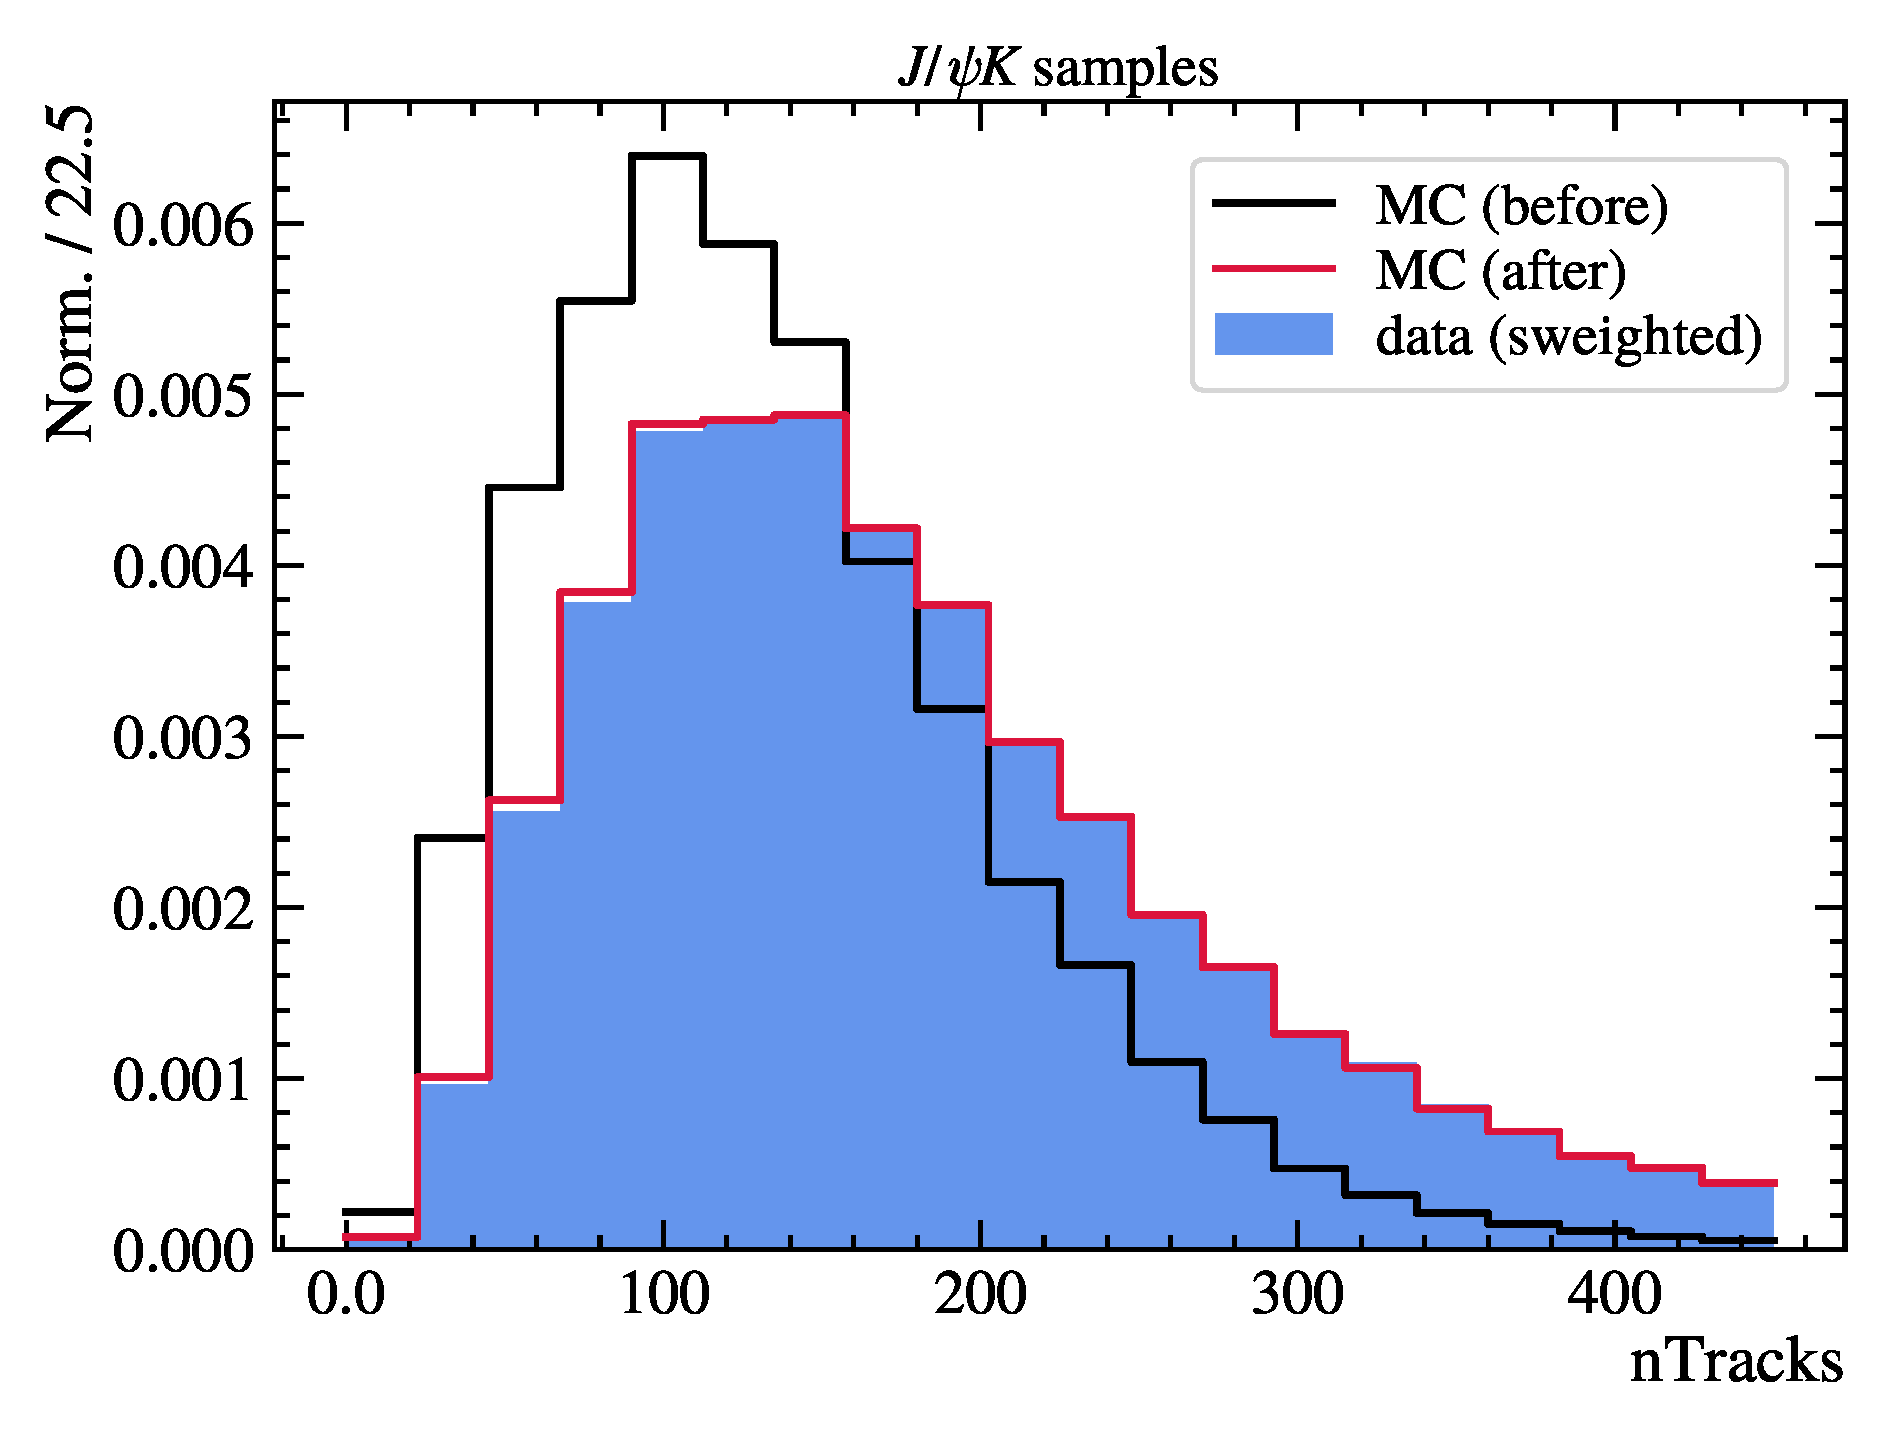
\includegraphics[width=0.45\textwidth]{./figs-mc-correction/reweighting-JpsiK/reweight-JpsiK/ntracks.pdf}
        \caption{Stage-1: $B$ PV ndf and nTracks.}
        \label{fig:rwt-JpsiK:stage1}
    \end{subfigure}

    \begin{subfigure}{\textwidth}
        \centering
        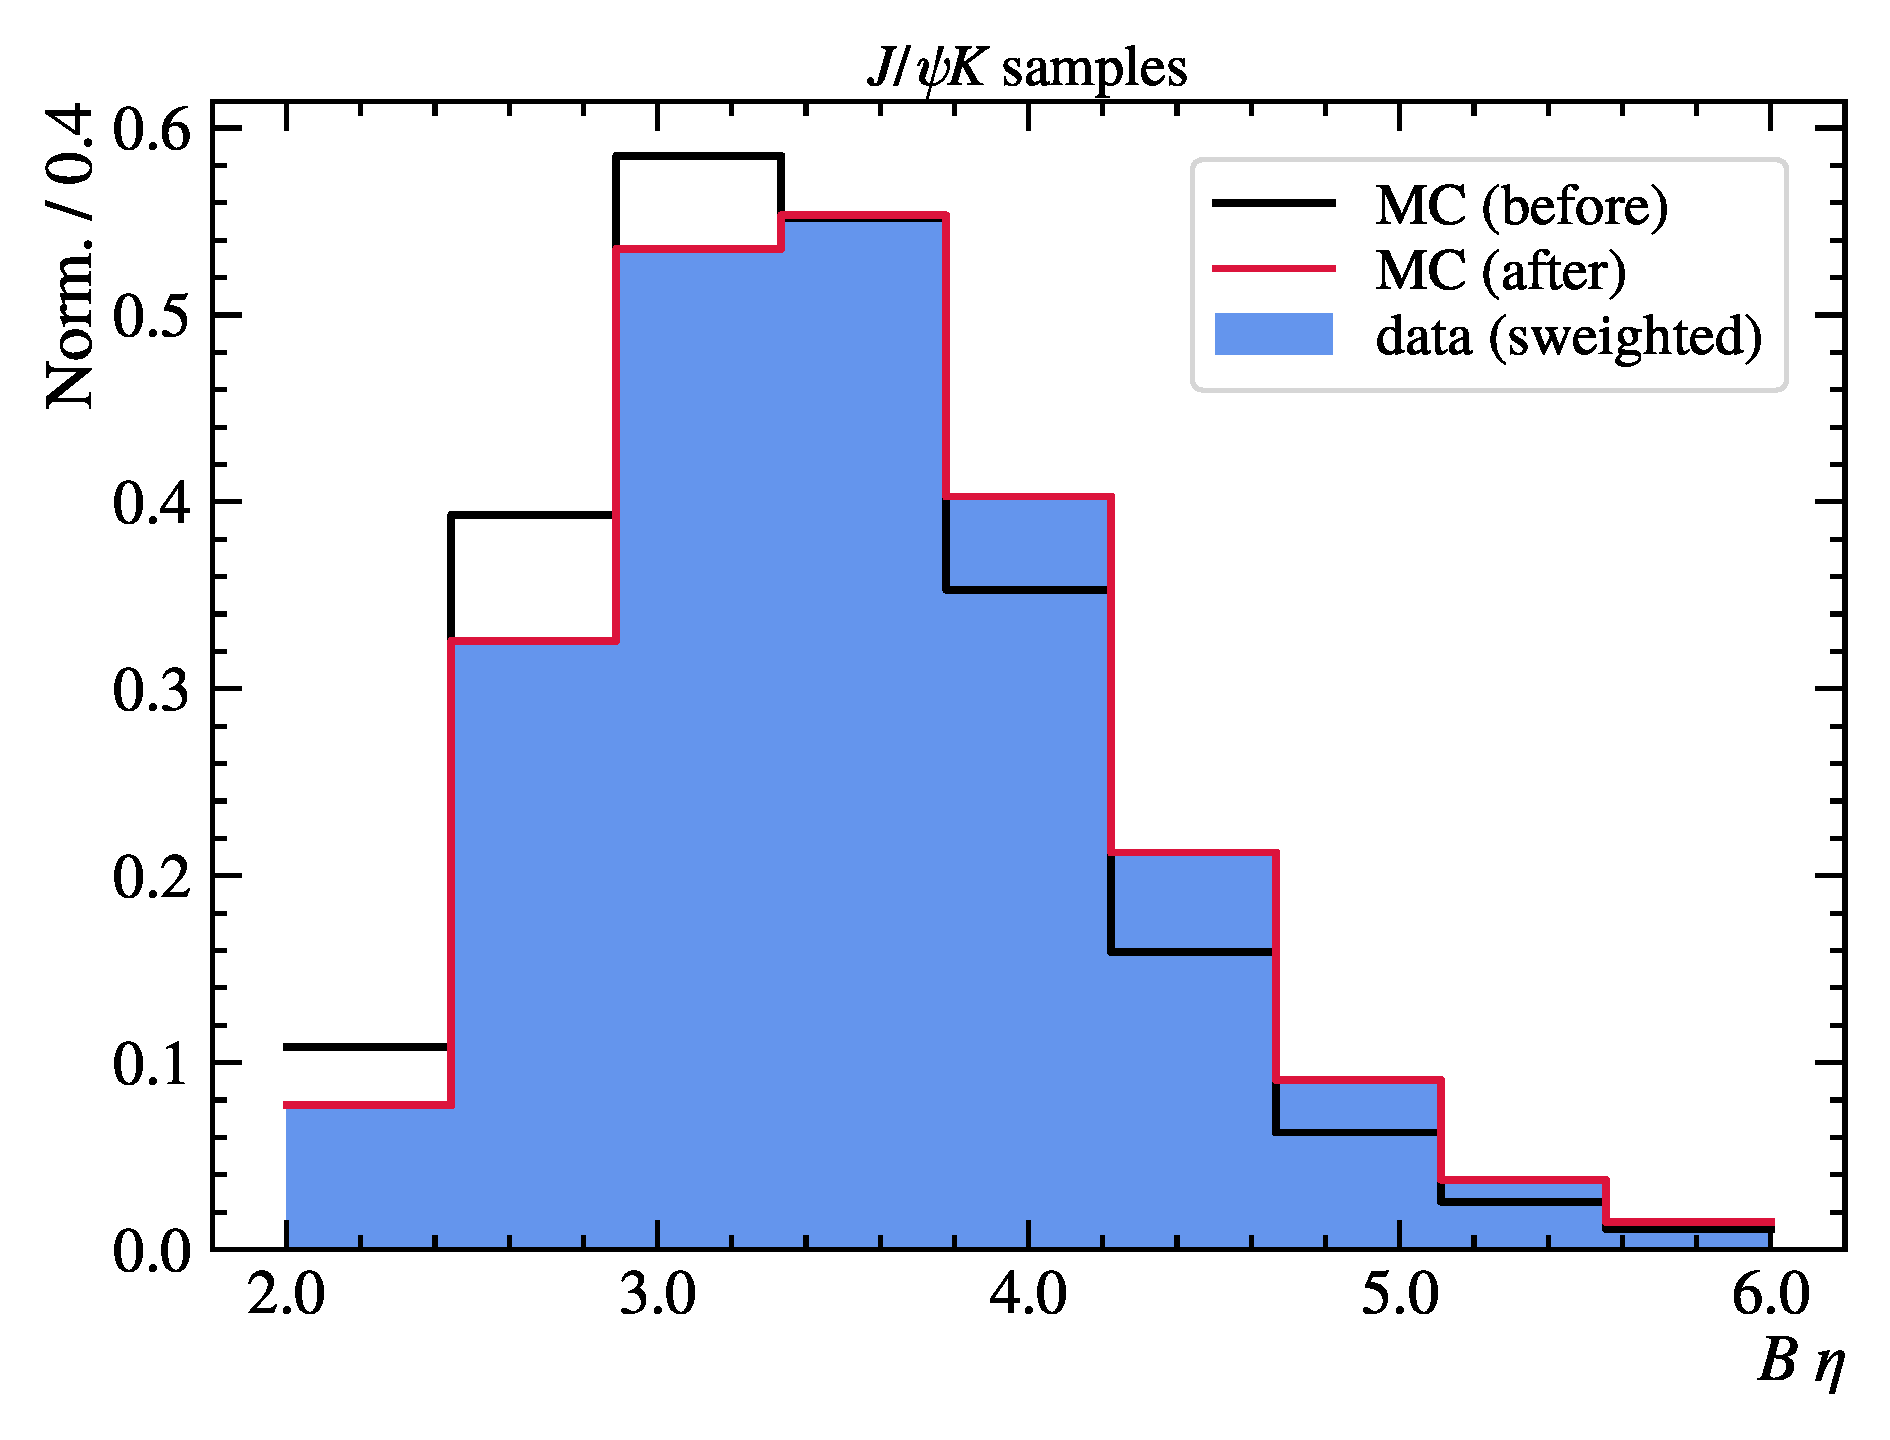
\includegraphics[width=0.45\textwidth]{./figs-mc-correction/reweighting-JpsiK/reweight-JpsiK/b_eta.pdf}
        \hspace{1em}
        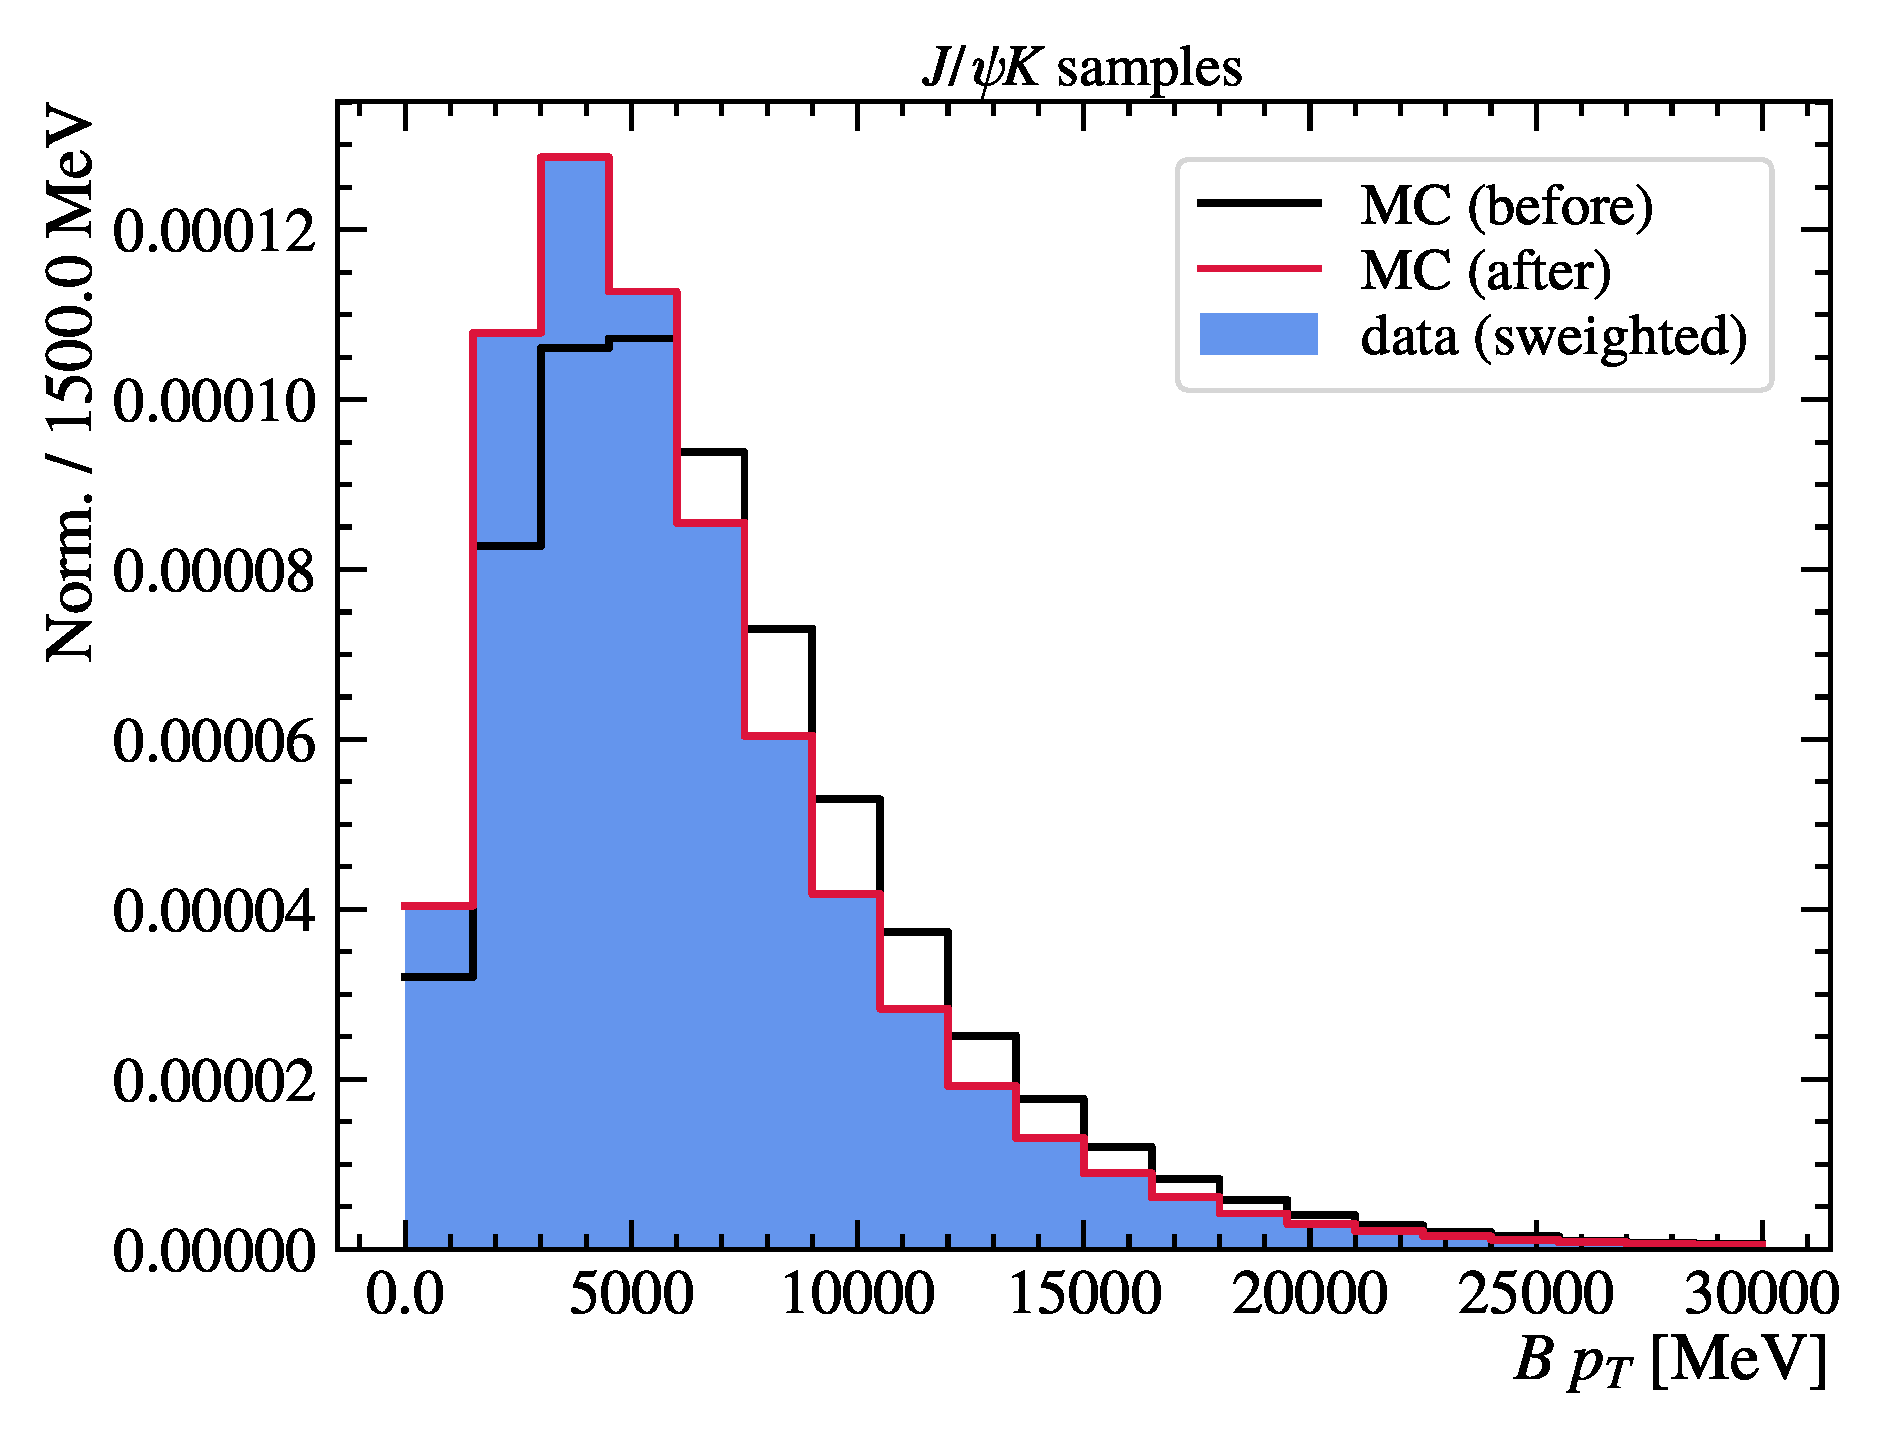
\includegraphics[width=0.45\textwidth]{./figs-mc-correction/reweighting-JpsiK/reweight-JpsiK/b_pt.pdf}
        \caption{Stage-2: $B$ $\eta$ and $B$ \pt.}
        \label{fig:rwt-JpsiK:stage2}
    \end{subfigure}

    \caption{
        Effect of \B kinematic and occupancy reweighting,
        derived from \jpsi\kaon control samples.
        The ``MC (after)'' plots contain corrections from \emph{all stages}.
    }
    \label{fig:rwt-JpsiK}
\end{figure}


\section{Post-fit cocktail}
\label{ref:mc-cor:postfit-cocktail}

To check data/MC agreements on many variables, a post-fit cocktail,
generated from scaling each fit component based its fitted yields, is needed.
This is because the selected data samples are themselves cocktails with
contributions from many decay modes, so no meaningful comparison between single
decay-mode MC and data can be performed.

After the initial weights are applied to the fit templates,
a multi-step fit,
termed \emph{initial fit},
which is identical to the \emph{canonical} fit described in
\cref{ref:fit:procedure},
is performed with initial-reweighted templates to determine the yield and
variations of each template.
The fit results are displayed in
\cref{appx:suppl:init-fit-cocktail}.

Since the main objective of final reweighting is to correct the remaining
inconsistencies between data and MC due to detector responses,
it is important to reweight in a region where most discrepancies are induced by
such responses.
Therefore, a $\mmSq < 0.4$ GeV$^2$ region,
termed reweighting region,
dominated in normalization decay mode,
mostly free of effects due to choice of modelling on background modes,
is used to derive the final weights.
The post-fit cocktail is built with the following procedure:

\begin{enumerate}
    \item Apply the $\mmSq < 0.4$ GeV$^2$ cut to obtain yields in the reweighting
        region based on total fitted yields.

    \item Some fit templates have variations which are specified by
        additionally provide variation templates at $\pm 1 \alpha$ and a
        interpolation/extrapolation method.
        More details can be seen in \cref{ref:fit:var}.

    \item After effecting possible variations,
        each fit template is rescaled such that the scaled integral of the
        template matches the fitted yield in the reweighting region.

    \item All MC templates are added together to form the
        \emph{post-fit cocktail}.
        The data-driven templates are subtracted from the \emph{data}
        template to form \emph{subtracted data} template
        which is comparable to the \emph{post-fit cocktail}.
\end{enumerate}


\section{Final reweighting}
\label{ref:mc-cor:final}

Final reweighting is a multi-stage reweighting process by comparing
selected kinematic and geometric variables of the \B decay daughters,
listed in \cref{tab:rwt-final-vars},
between \emph{post-fit cocktail} and \emph{subtracted data}
in the reweighting region, selected by a $\mmSq < 0.4$ GeV$^2$ cut,
and generate binned $\frac{\text{data}}{\text{MC}}$ ratios as weights for each
variable.
The reweighting is performed separately for \Dz and \Dstar channel;
the latter contains additional stages due to corrections to slow \pion.

The effects of final reweighting can be seen at
\cref{fig:final-rwt-d0-idx0,fig:final-rwt-d0-idx1,fig:final-rwt-d0-idx2,fig:final-rwt-d0-idx3}
for \Dz channel, and
\cref{fig:final-rwt-dst-idx0,fig:final-rwt-dst-idx1,fig:final-rwt-dst-idx2,fig:final-rwt-dst-idx3}
for \Dstar channel.
Some important technical details are provided below.

\paragraph{Bins with 0 MC event} For bins without MC events,
the weights are replaced by 1, to avoid arbitrarily large weights.
This is justified by the fact that if the corresponding data bins also have
0 event, no reweighting is needed;
otherwise it is likely that large weights will be produced by the reweighting
procedure and it is the case we want to avoided.

\paragraph{Treatment of large weights}
For large weights, defined as $w \geq 50$, the number of events $n$
in the corresponding bin of the \emph{subtracted data} sample is checked:
If $n \leq 10$, the large weight is treated as a fluctuation and is
set back to 1;
otherwise, it is capped at 50.
No other weight cap is imposed on the \jpsi\kaon-derived weight at this
stage\footnote{
    There are, however, weight caps on the products of weights,
    which will be described in
    \cref{ref:fit:tmpl}.
}.

\paragraph{Under and overflow bins}
The under and overflow bins are taken into account during
the reweighting process.


\begin{figure}[htb]
    \begin{subfigure}{\textwidth}
        \centering
        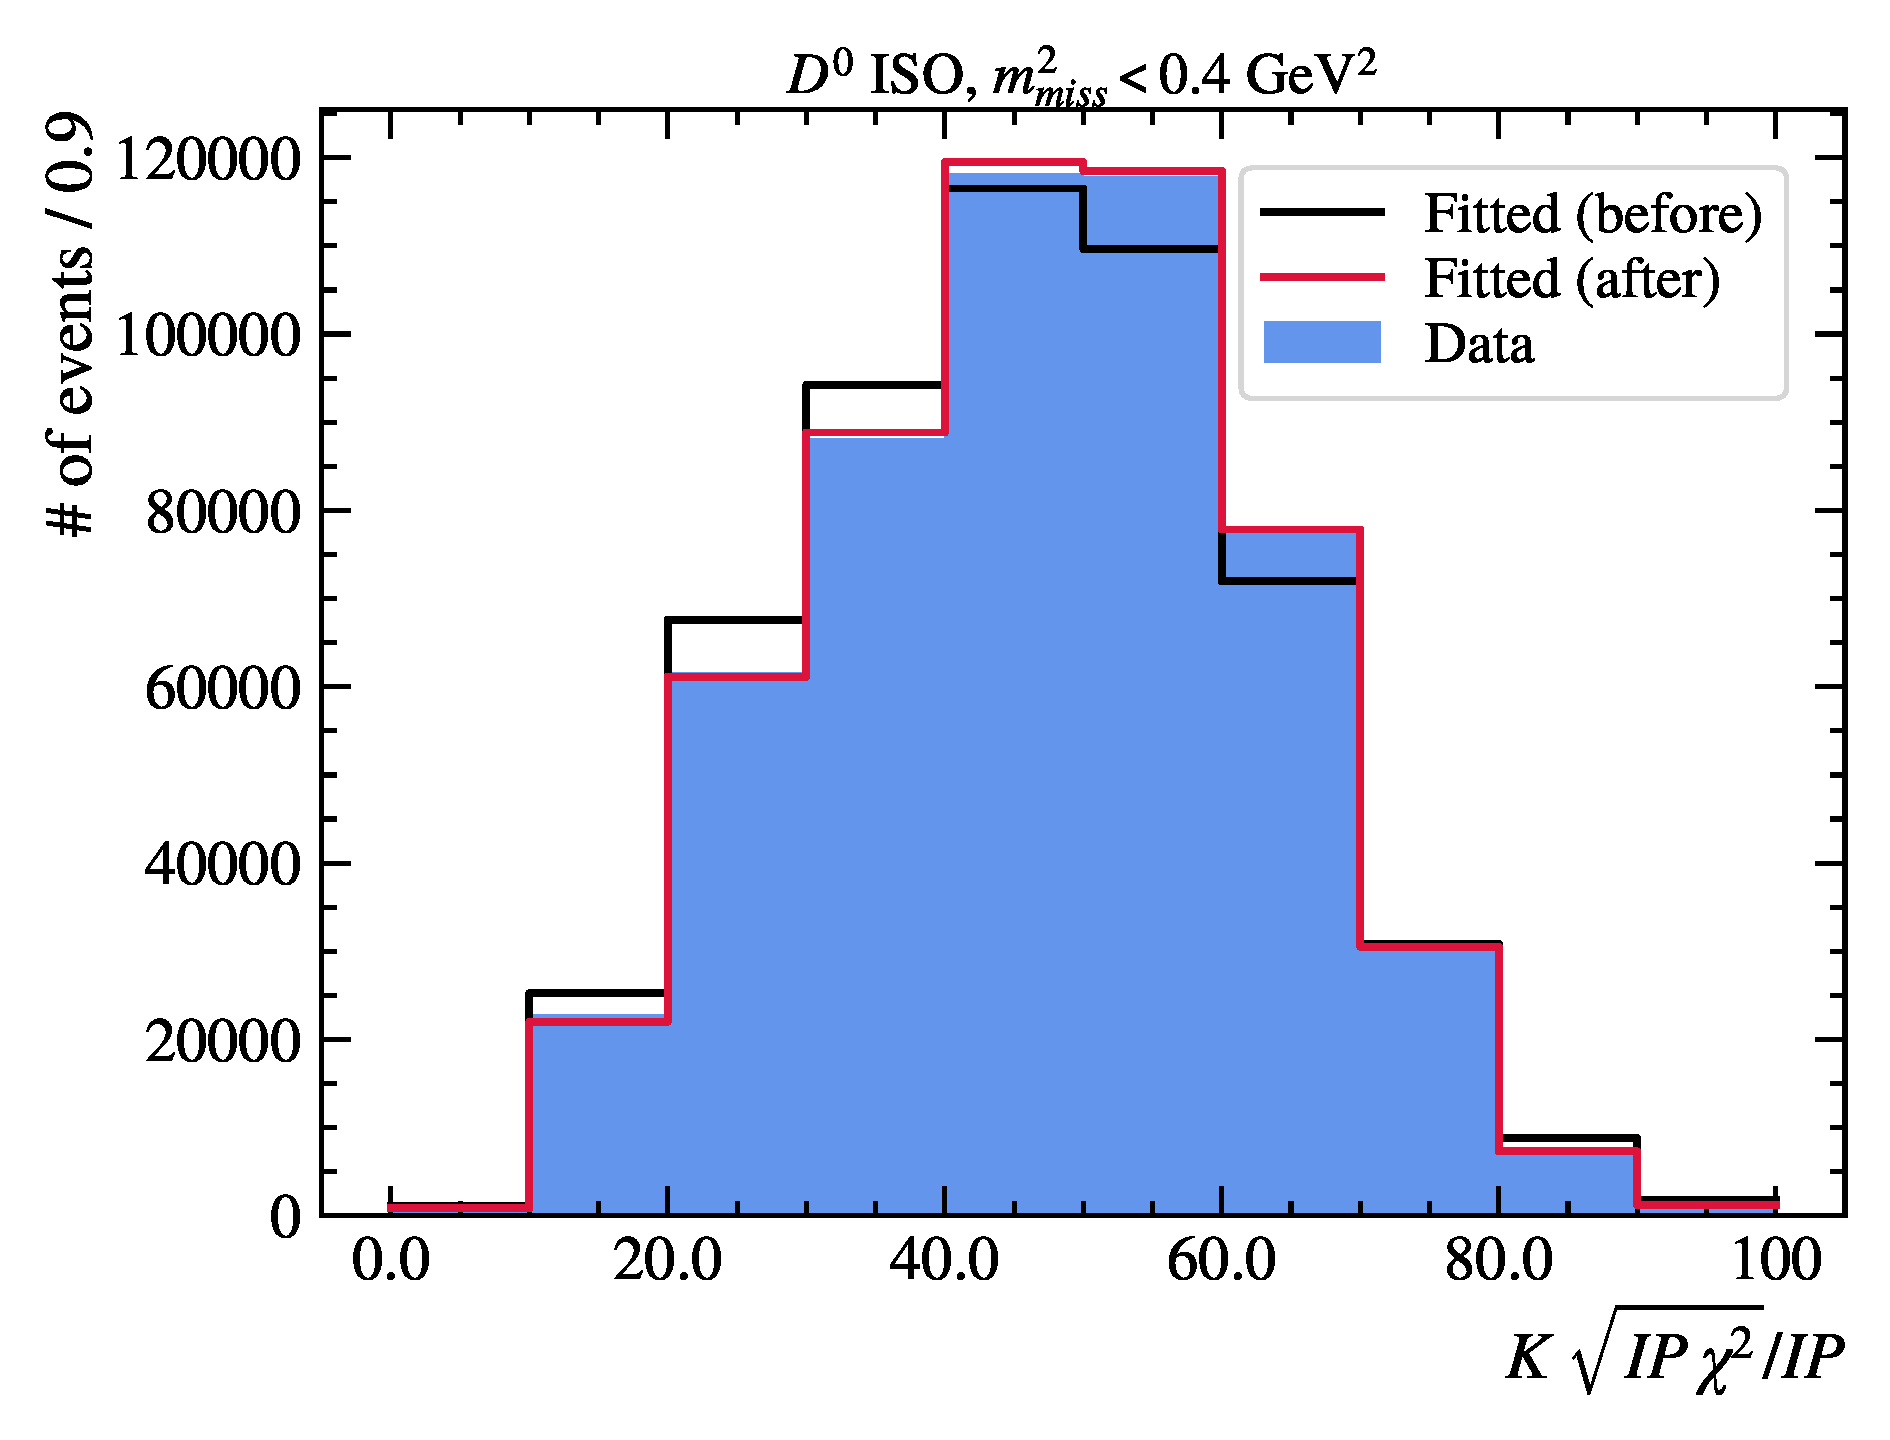
\includegraphics[width=0.32\textwidth]{./figs-mc-correction/reweighting-final/plot_step0-D0_iso-k_comp.pdf}
        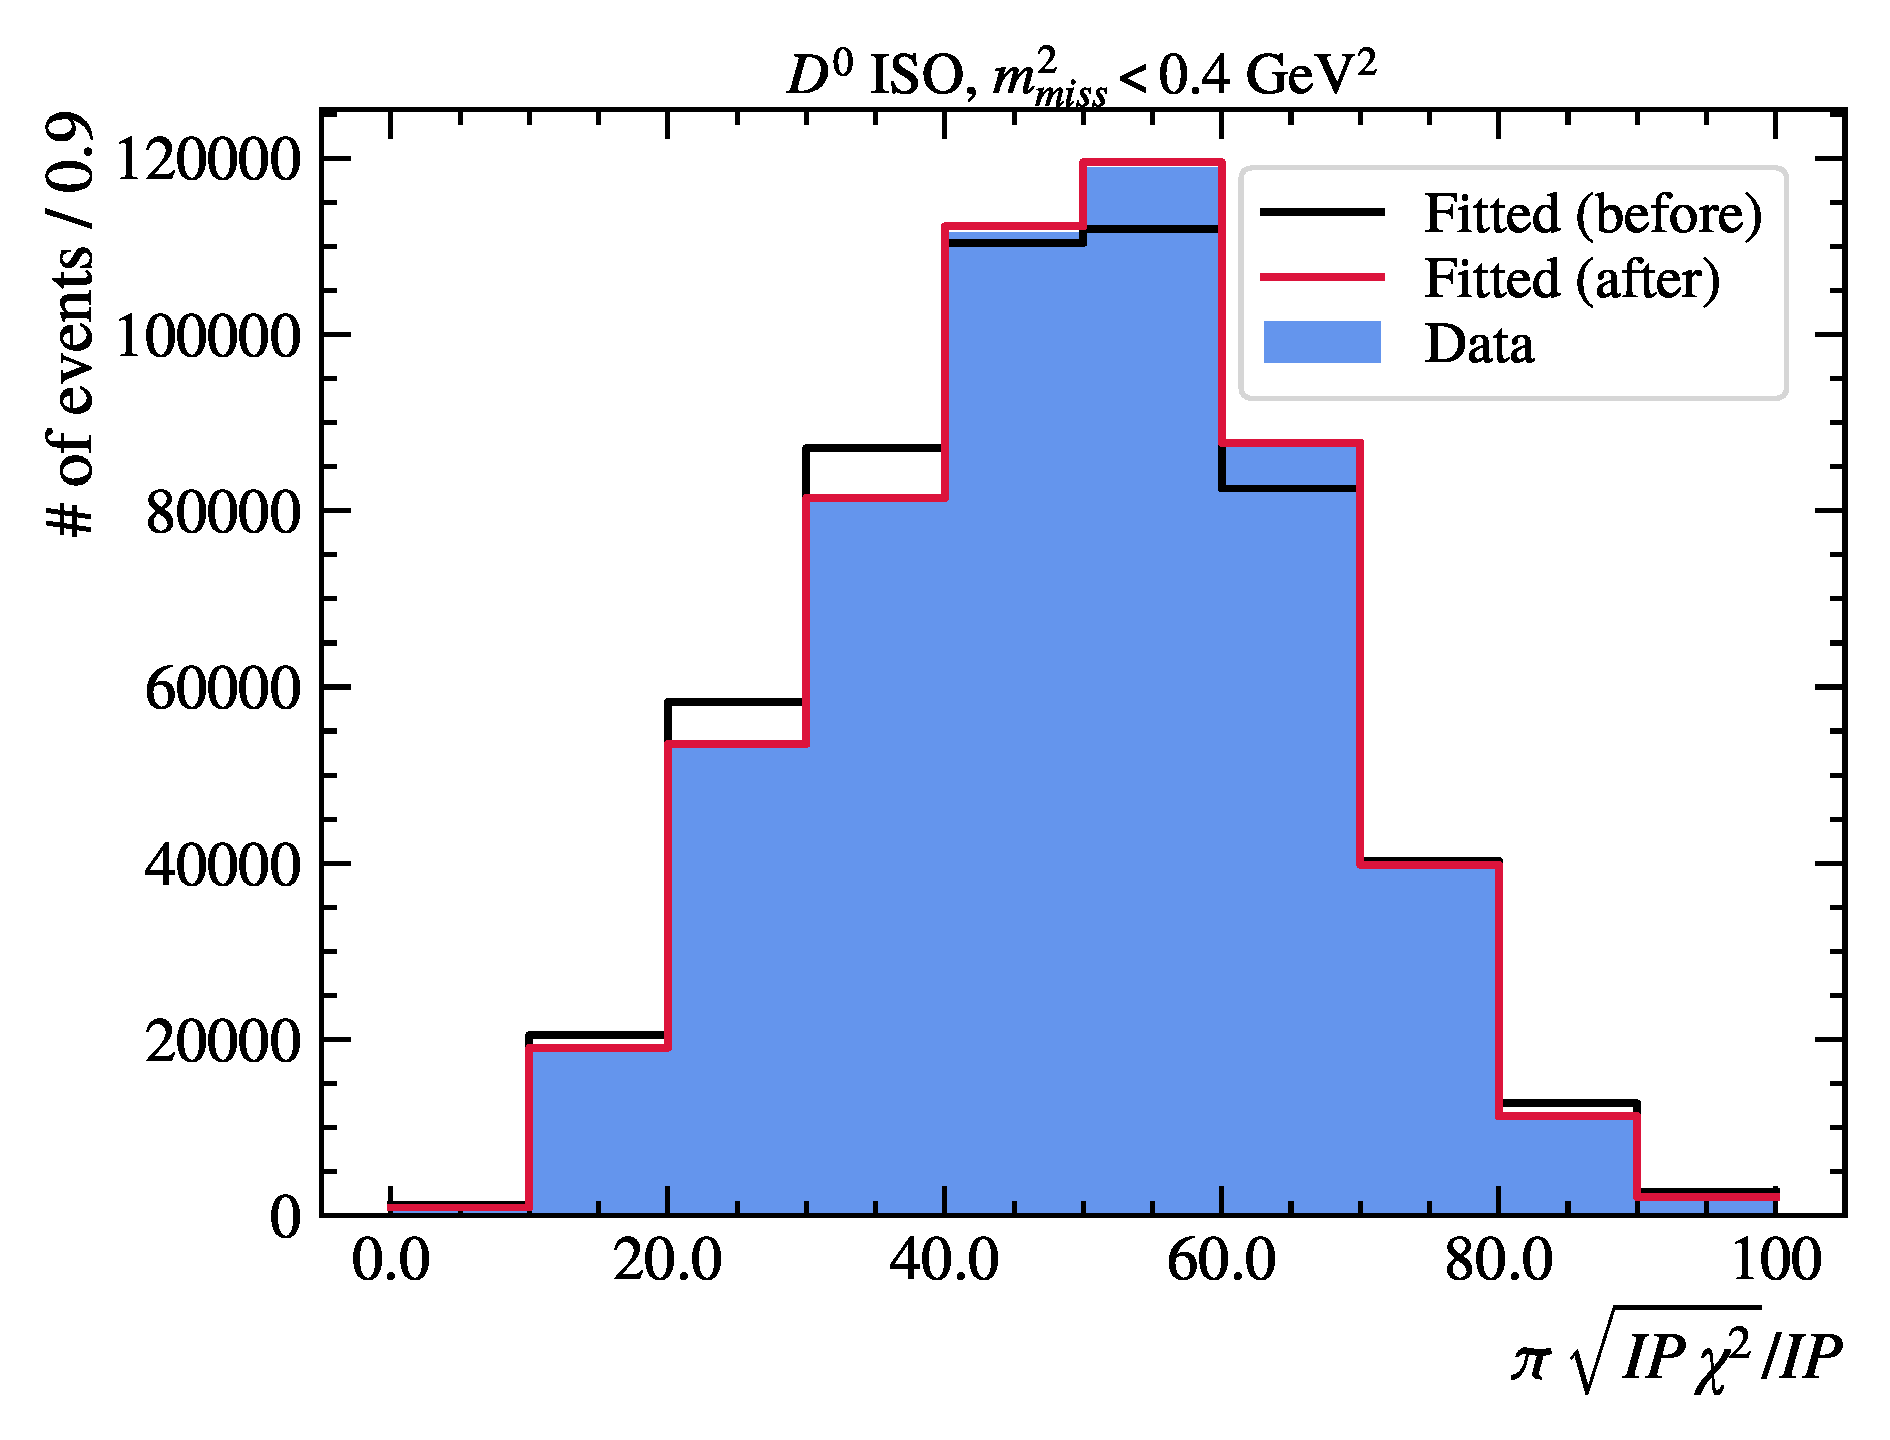
\includegraphics[width=0.32\textwidth]{./figs-mc-correction/reweighting-final/plot_step0-D0_iso-pi_comp.pdf}
        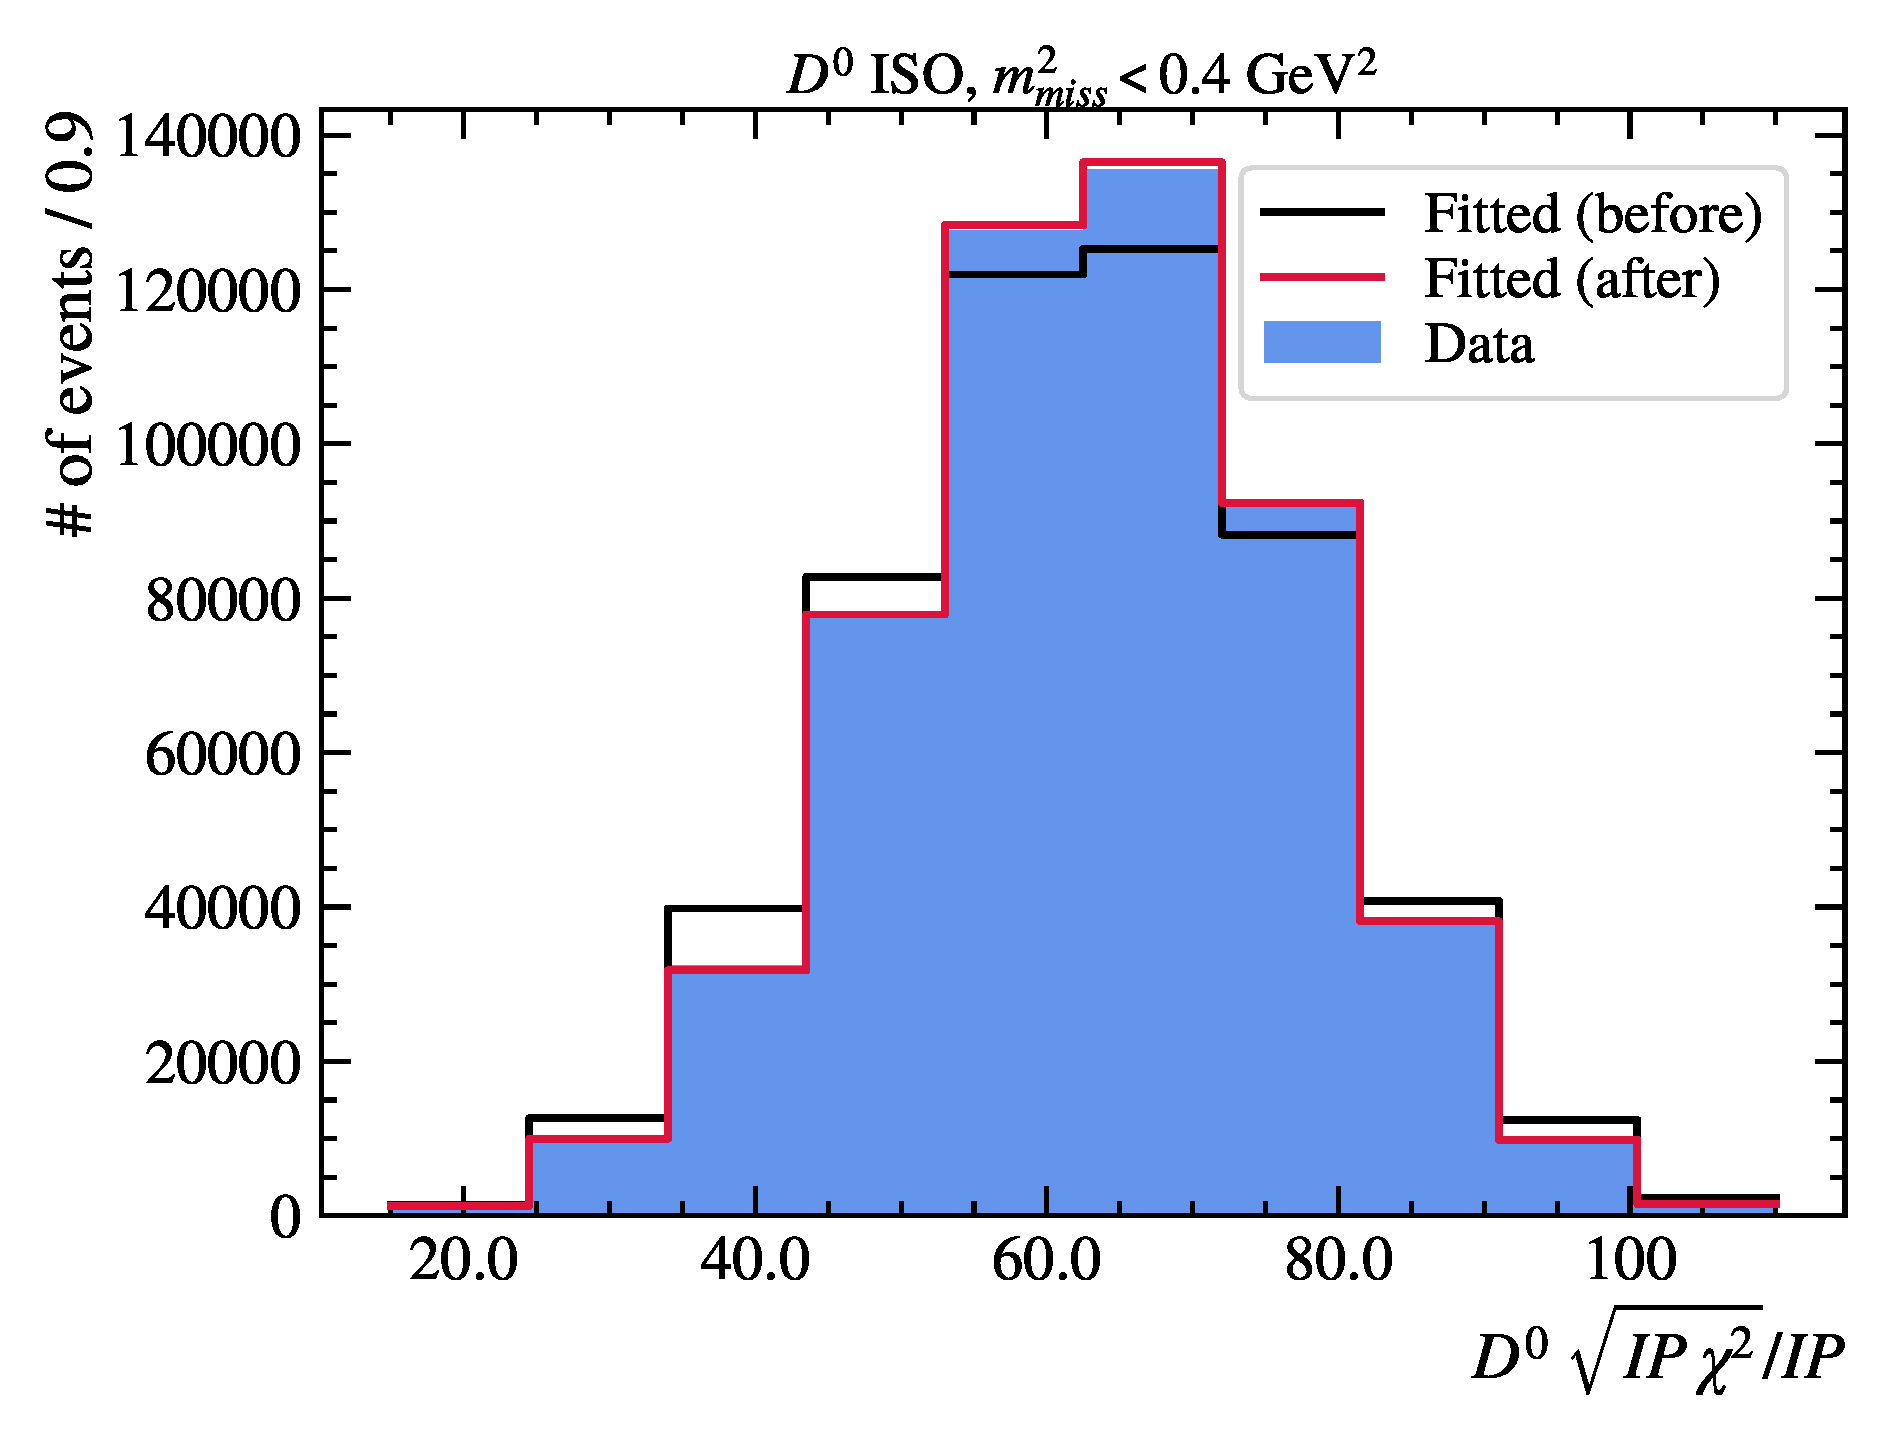
\includegraphics[width=0.32\textwidth]{./figs-mc-correction/reweighting-final/plot_step0-D0_iso-d0_comp.pdf}
        \caption{Stage 1.}
    \end{subfigure}
    \caption{
        Final reweighting for \Dz channel, for a total of 11 stages.
        The black plots contain weights from \emph{all previous} stages,
        whereas the red ones contain weights from \emph{all} stages.
    }
    \label{fig:final-rwt-d0-idx0}
\end{figure}

\begin{figure}[htb]
    \begin{subfigure}{\textwidth}
        \centering
        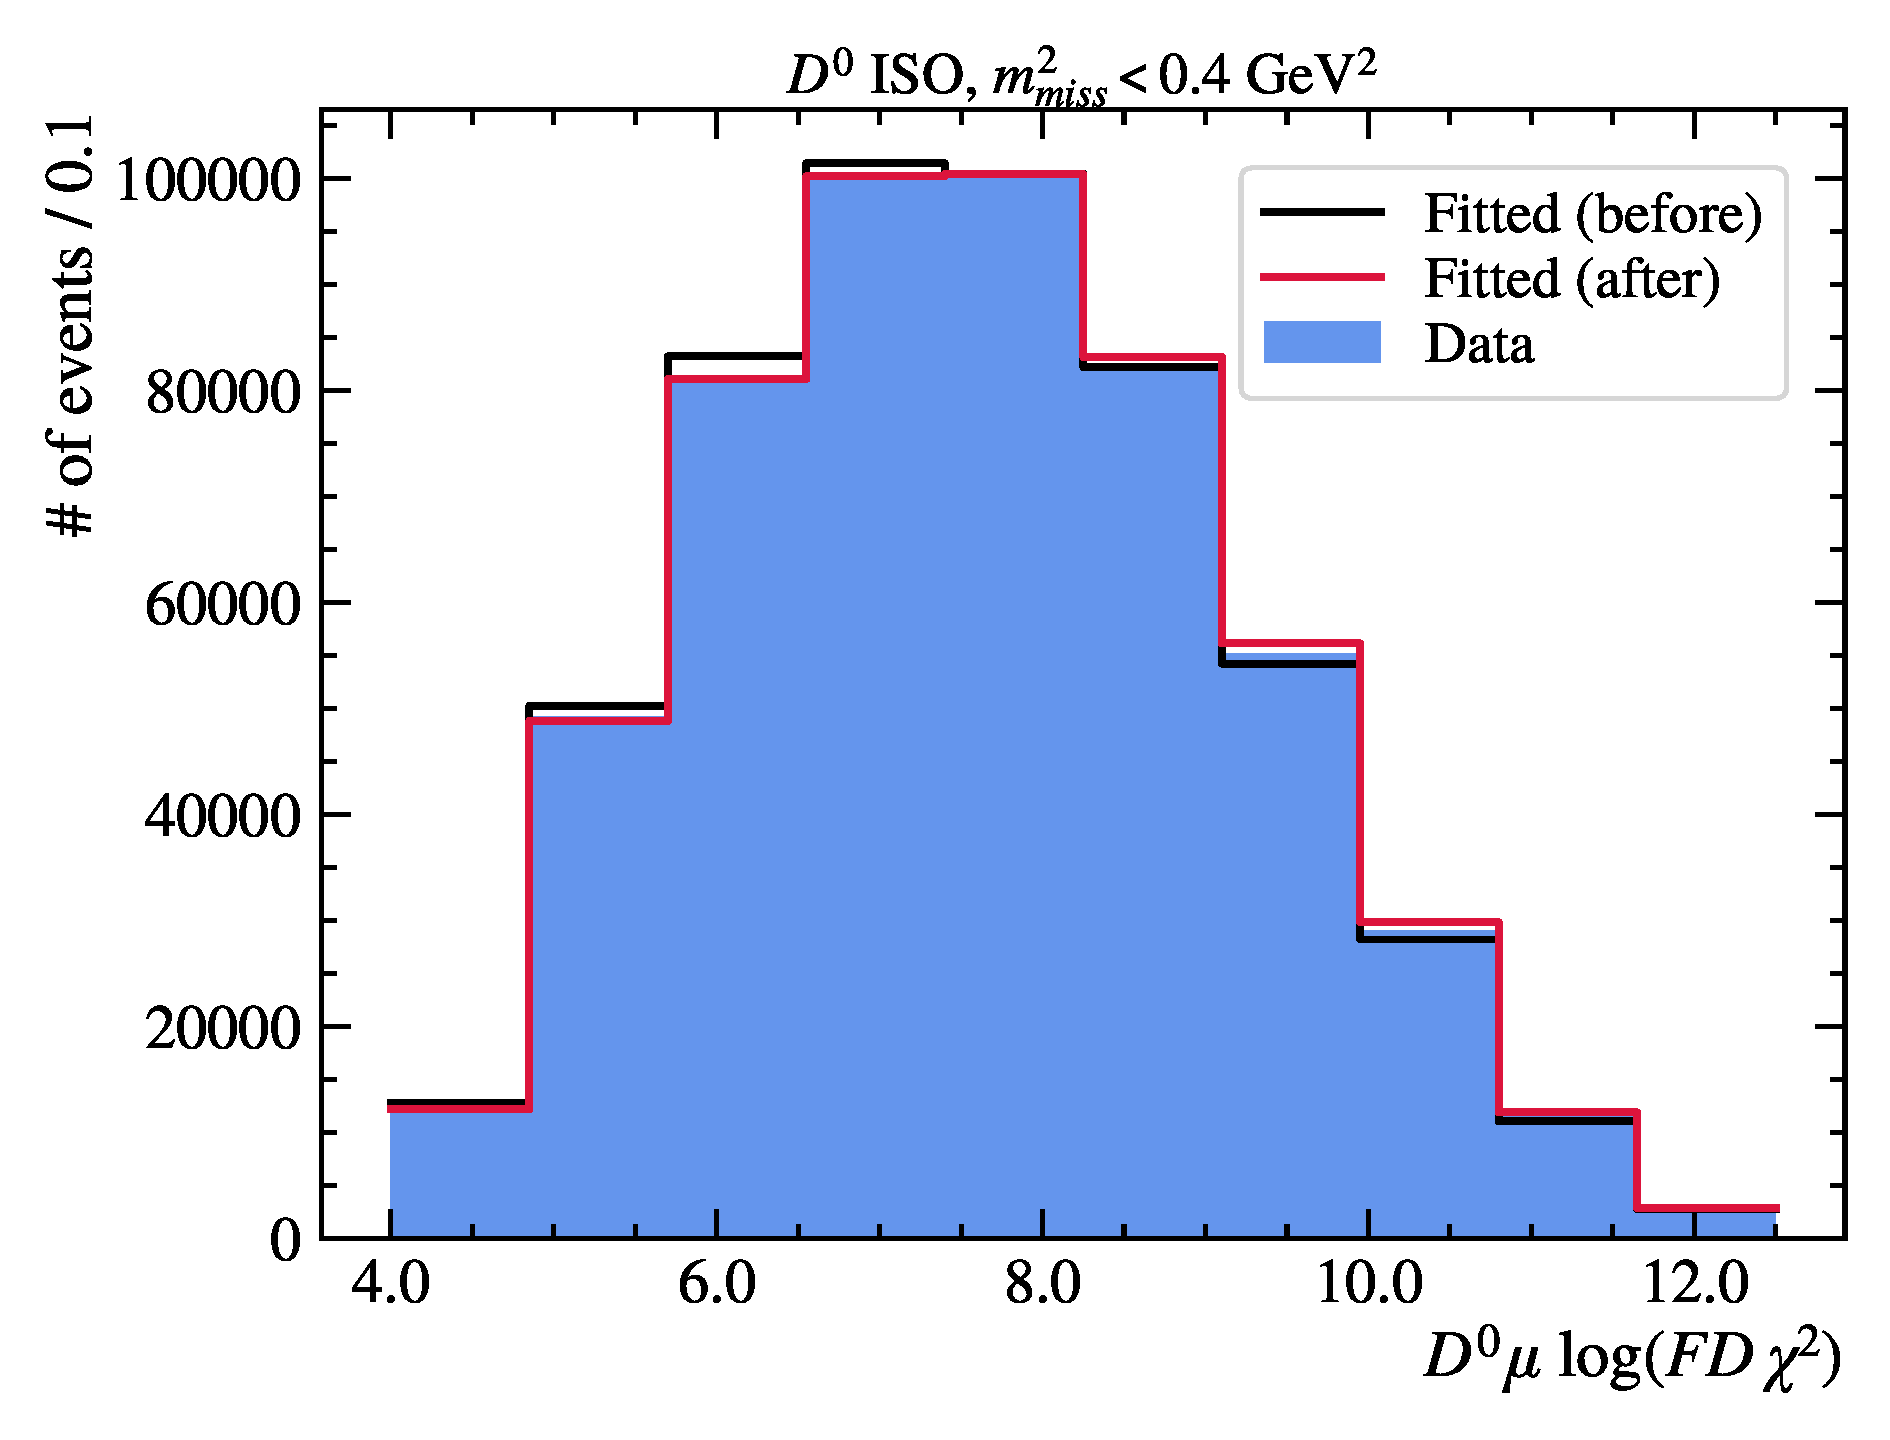
\includegraphics[width=0.32\textwidth]{./figs-mc-correction/reweighting-final/plot_step1-D0_iso-b_log_fd_chi2.pdf}
        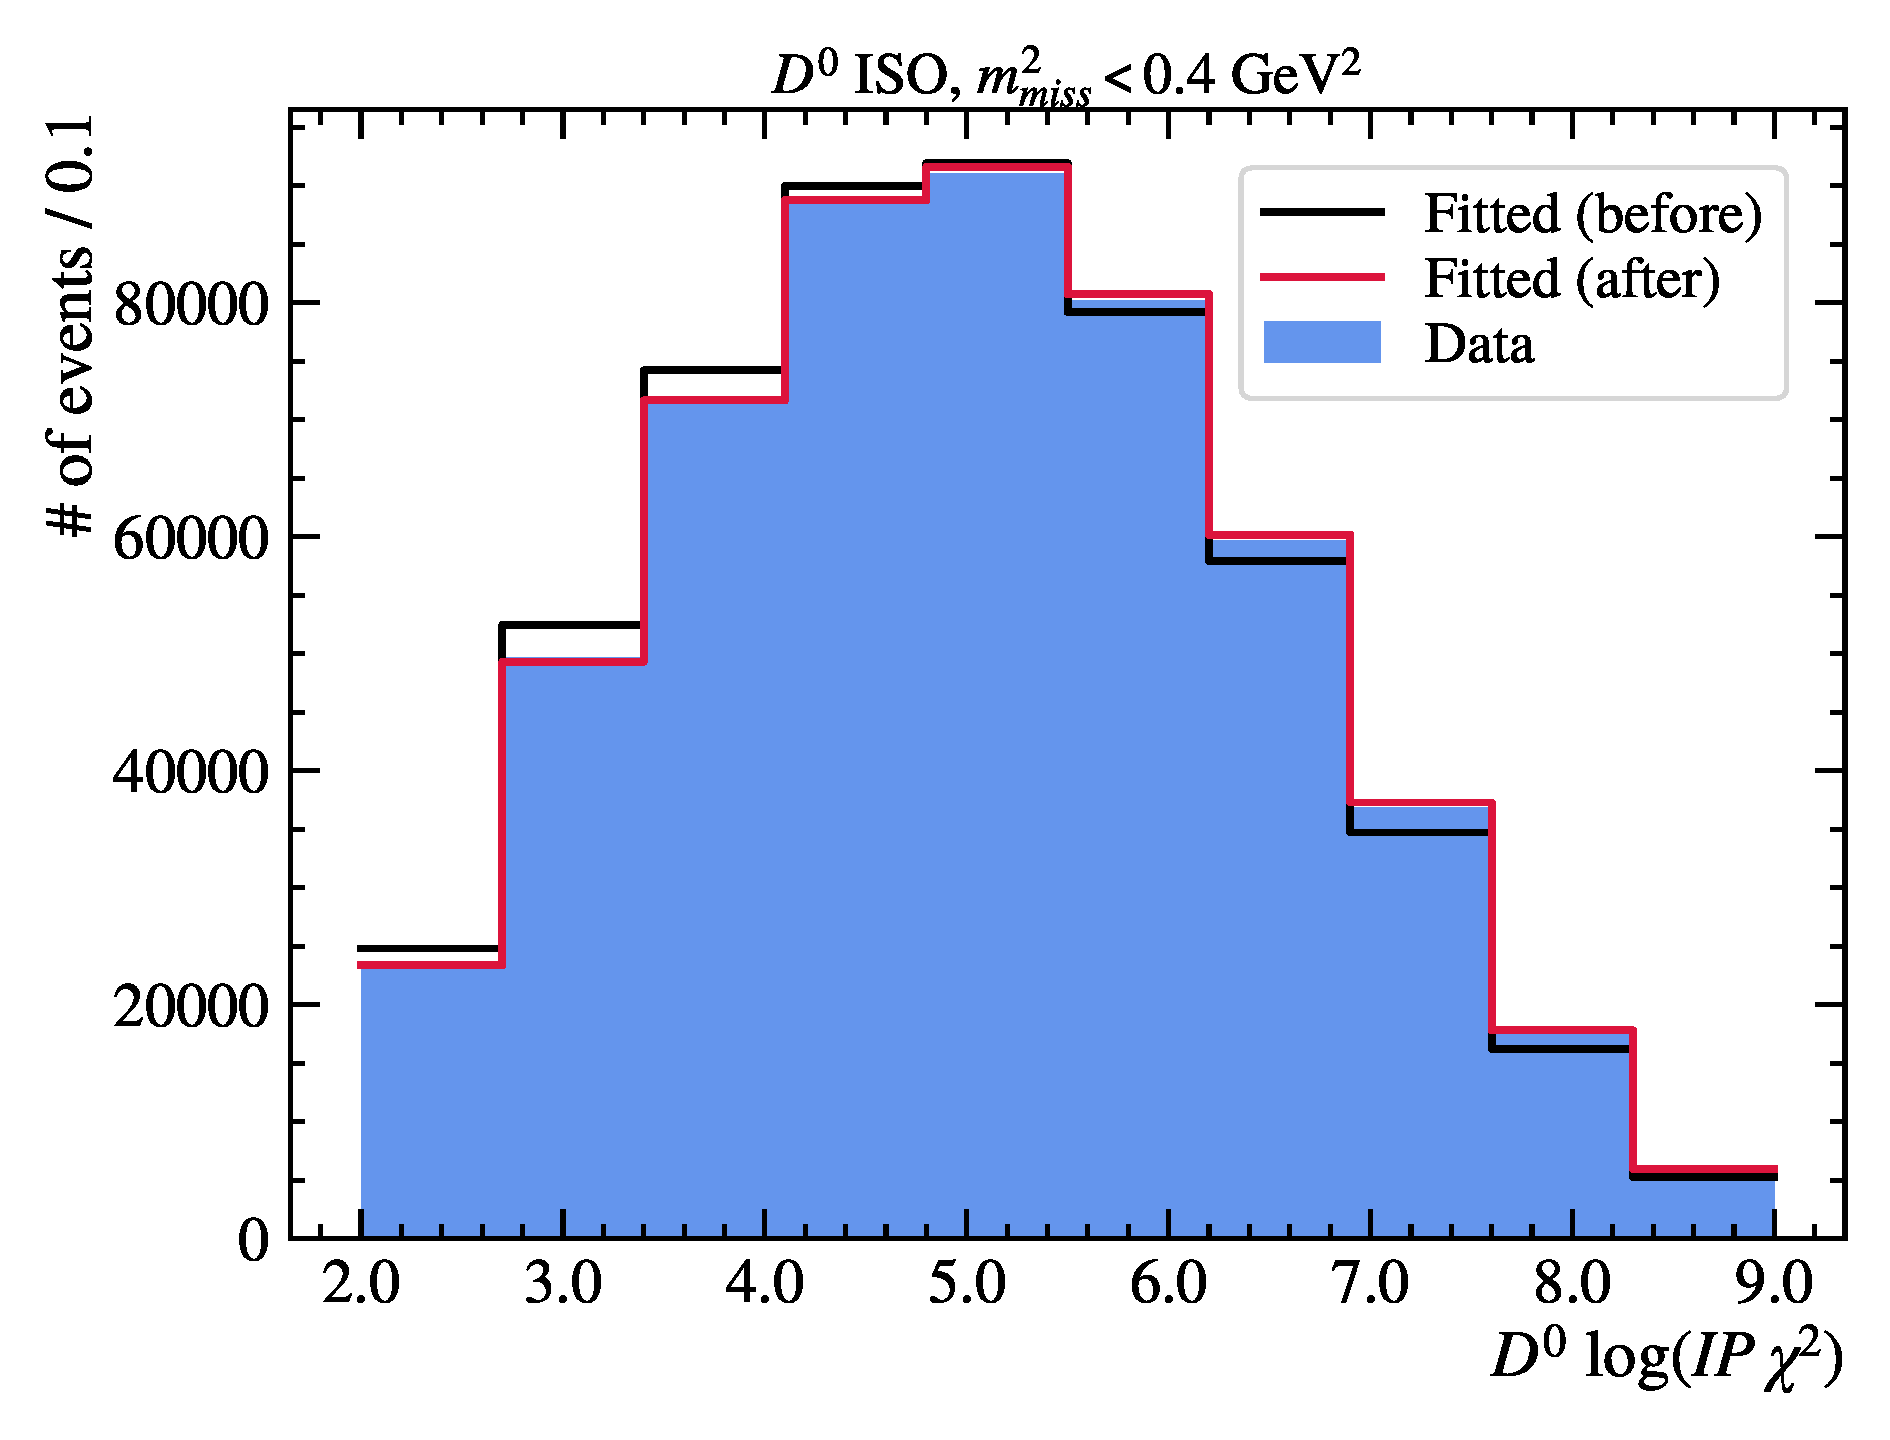
\includegraphics[width=0.32\textwidth]{./figs-mc-correction/reweighting-final/plot_step1-D0_iso-d0_log_ip_chi2.pdf}
        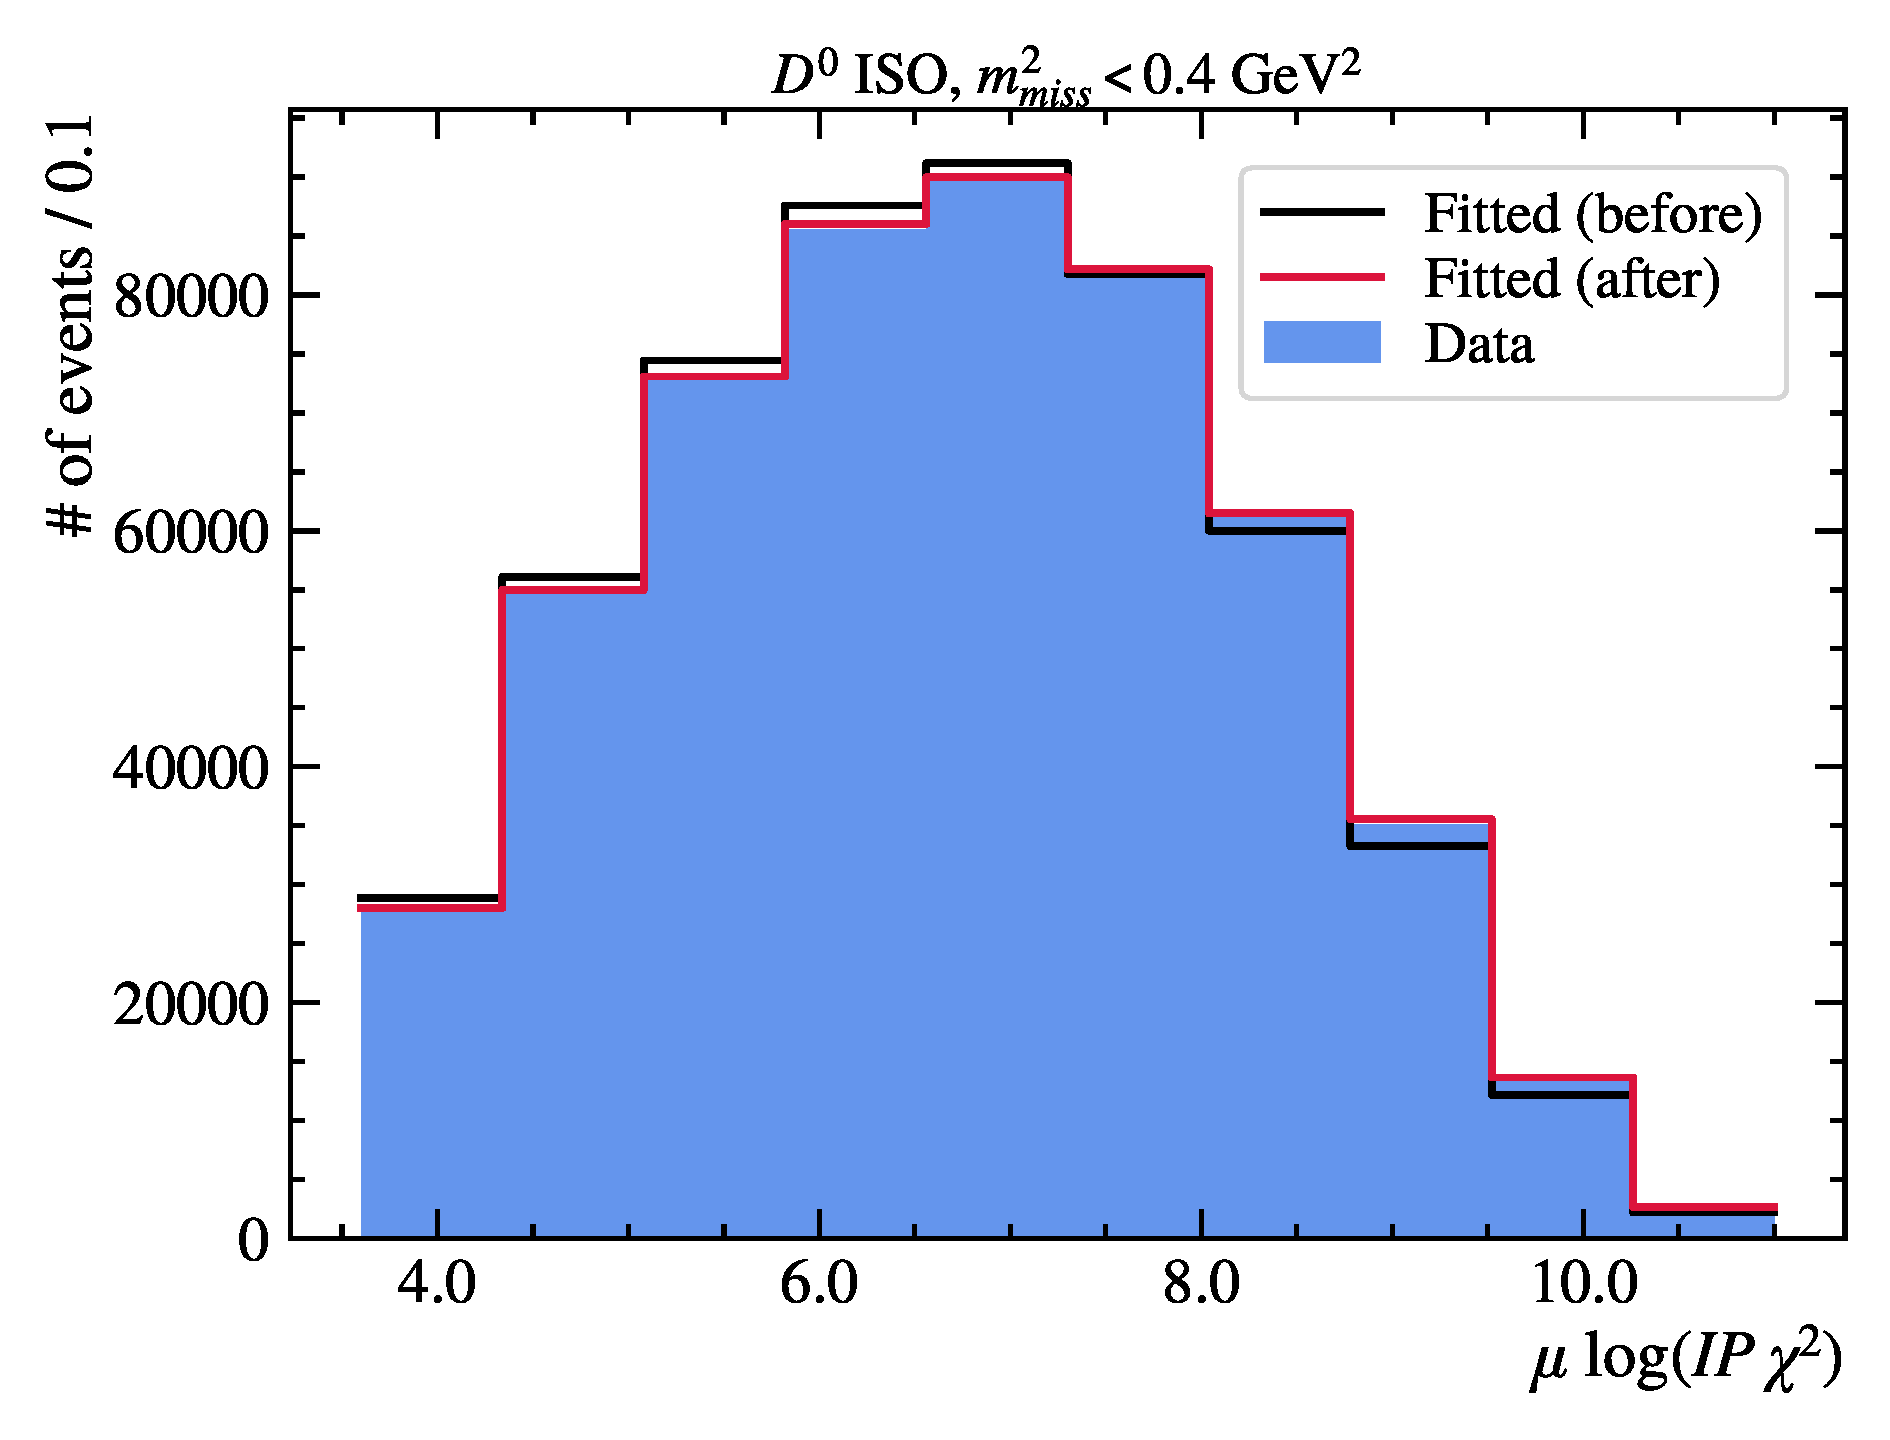
\includegraphics[width=0.32\textwidth]{./figs-mc-correction/reweighting-final/plot_step1-D0_iso-mu_log_ip_chi2.pdf}
        \caption{Stage 2.}
    \end{subfigure}

    \begin{subfigure}{\textwidth}
        \centering
        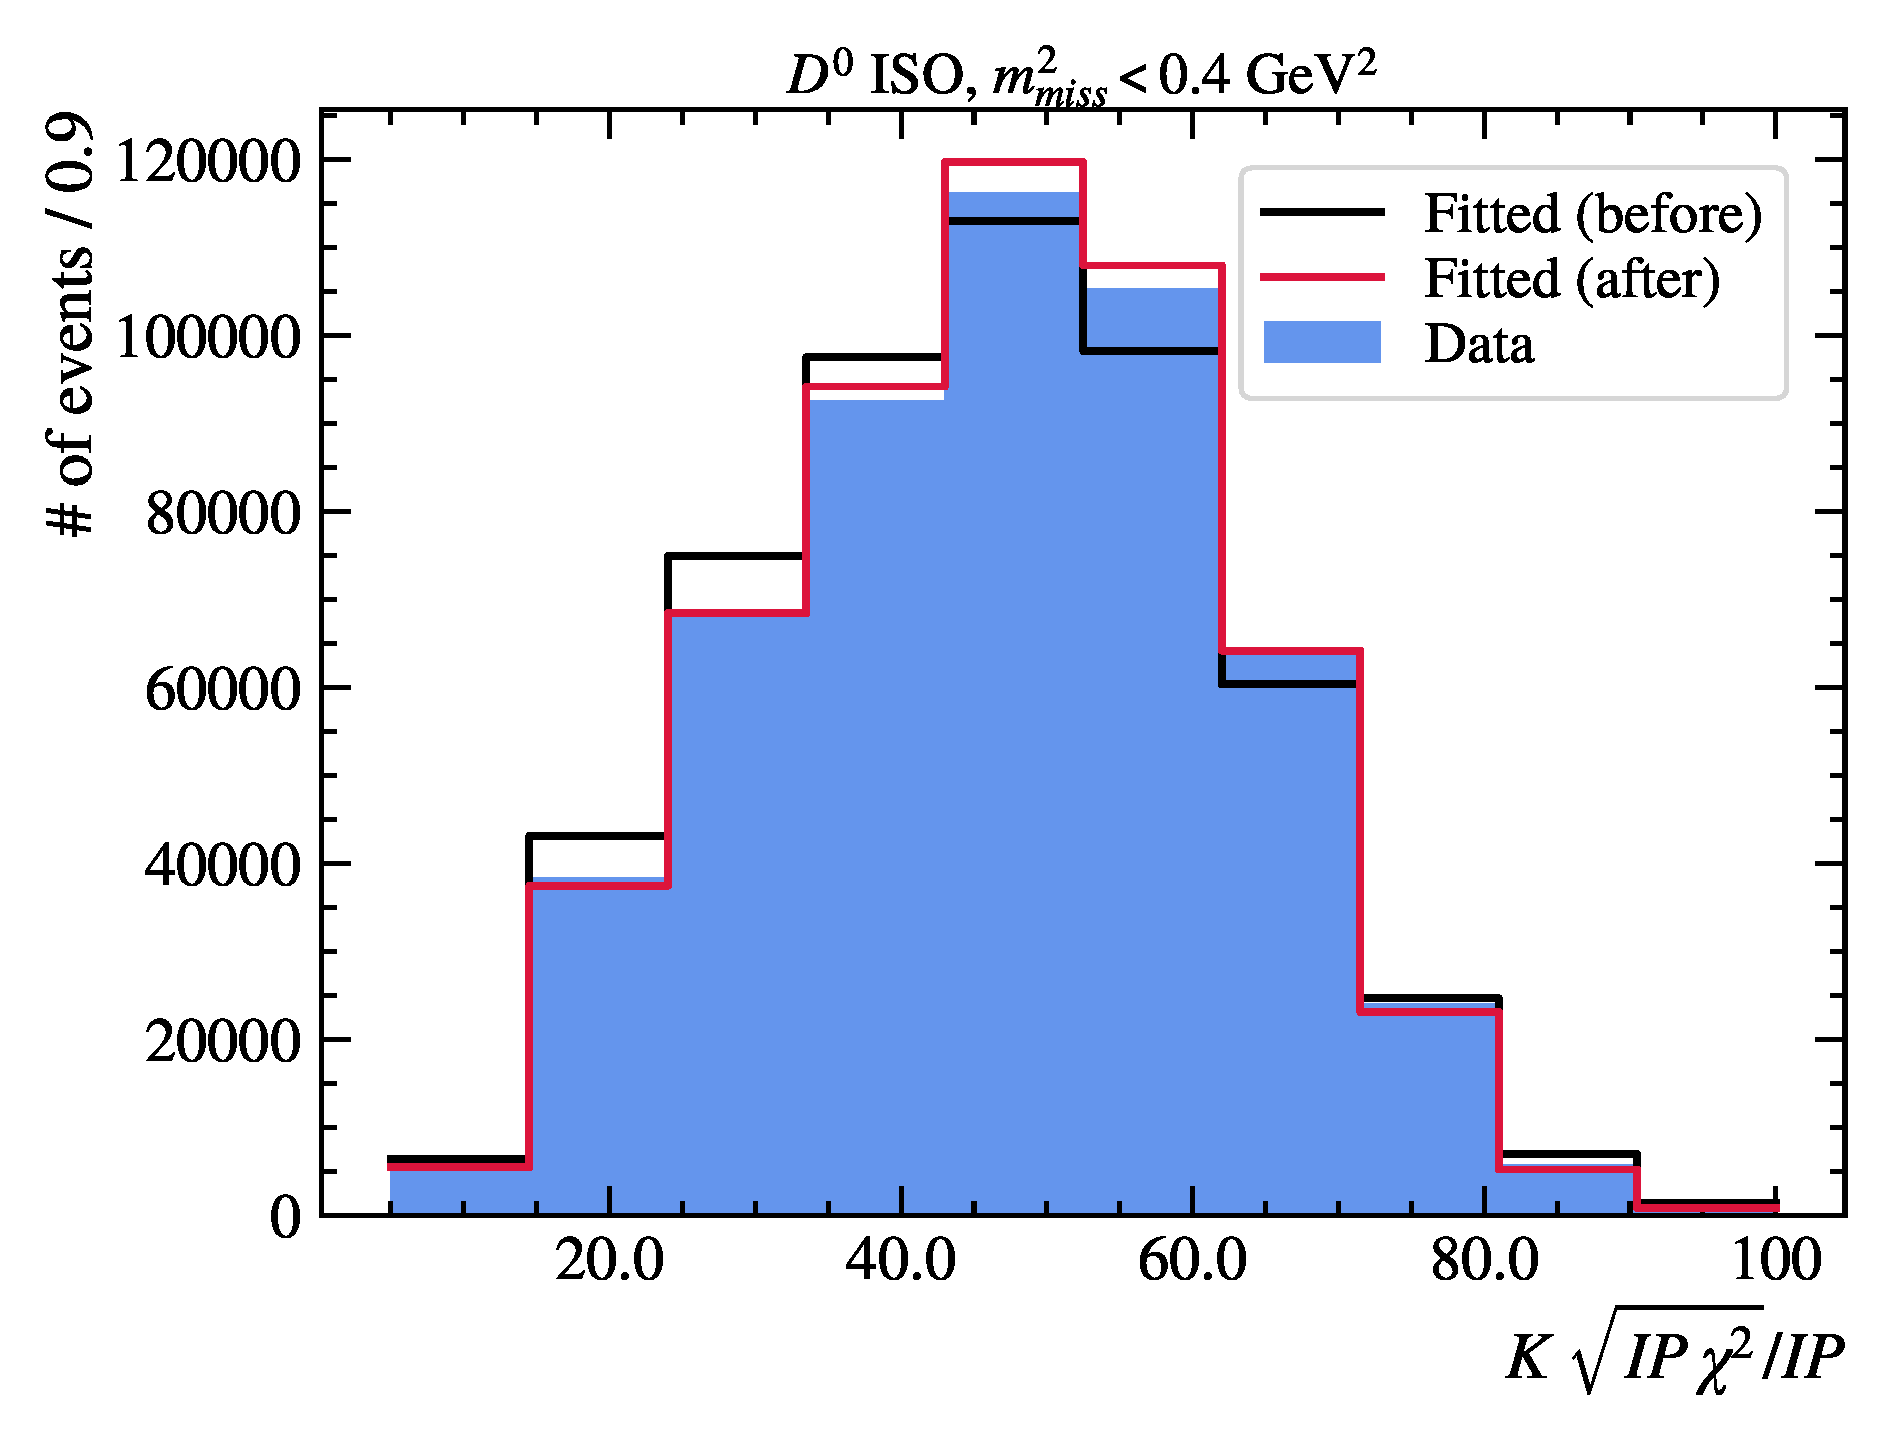
\includegraphics[width=0.32\textwidth]{./figs-mc-correction/reweighting-final/plot_step2-D0_iso-k_comp.pdf}
        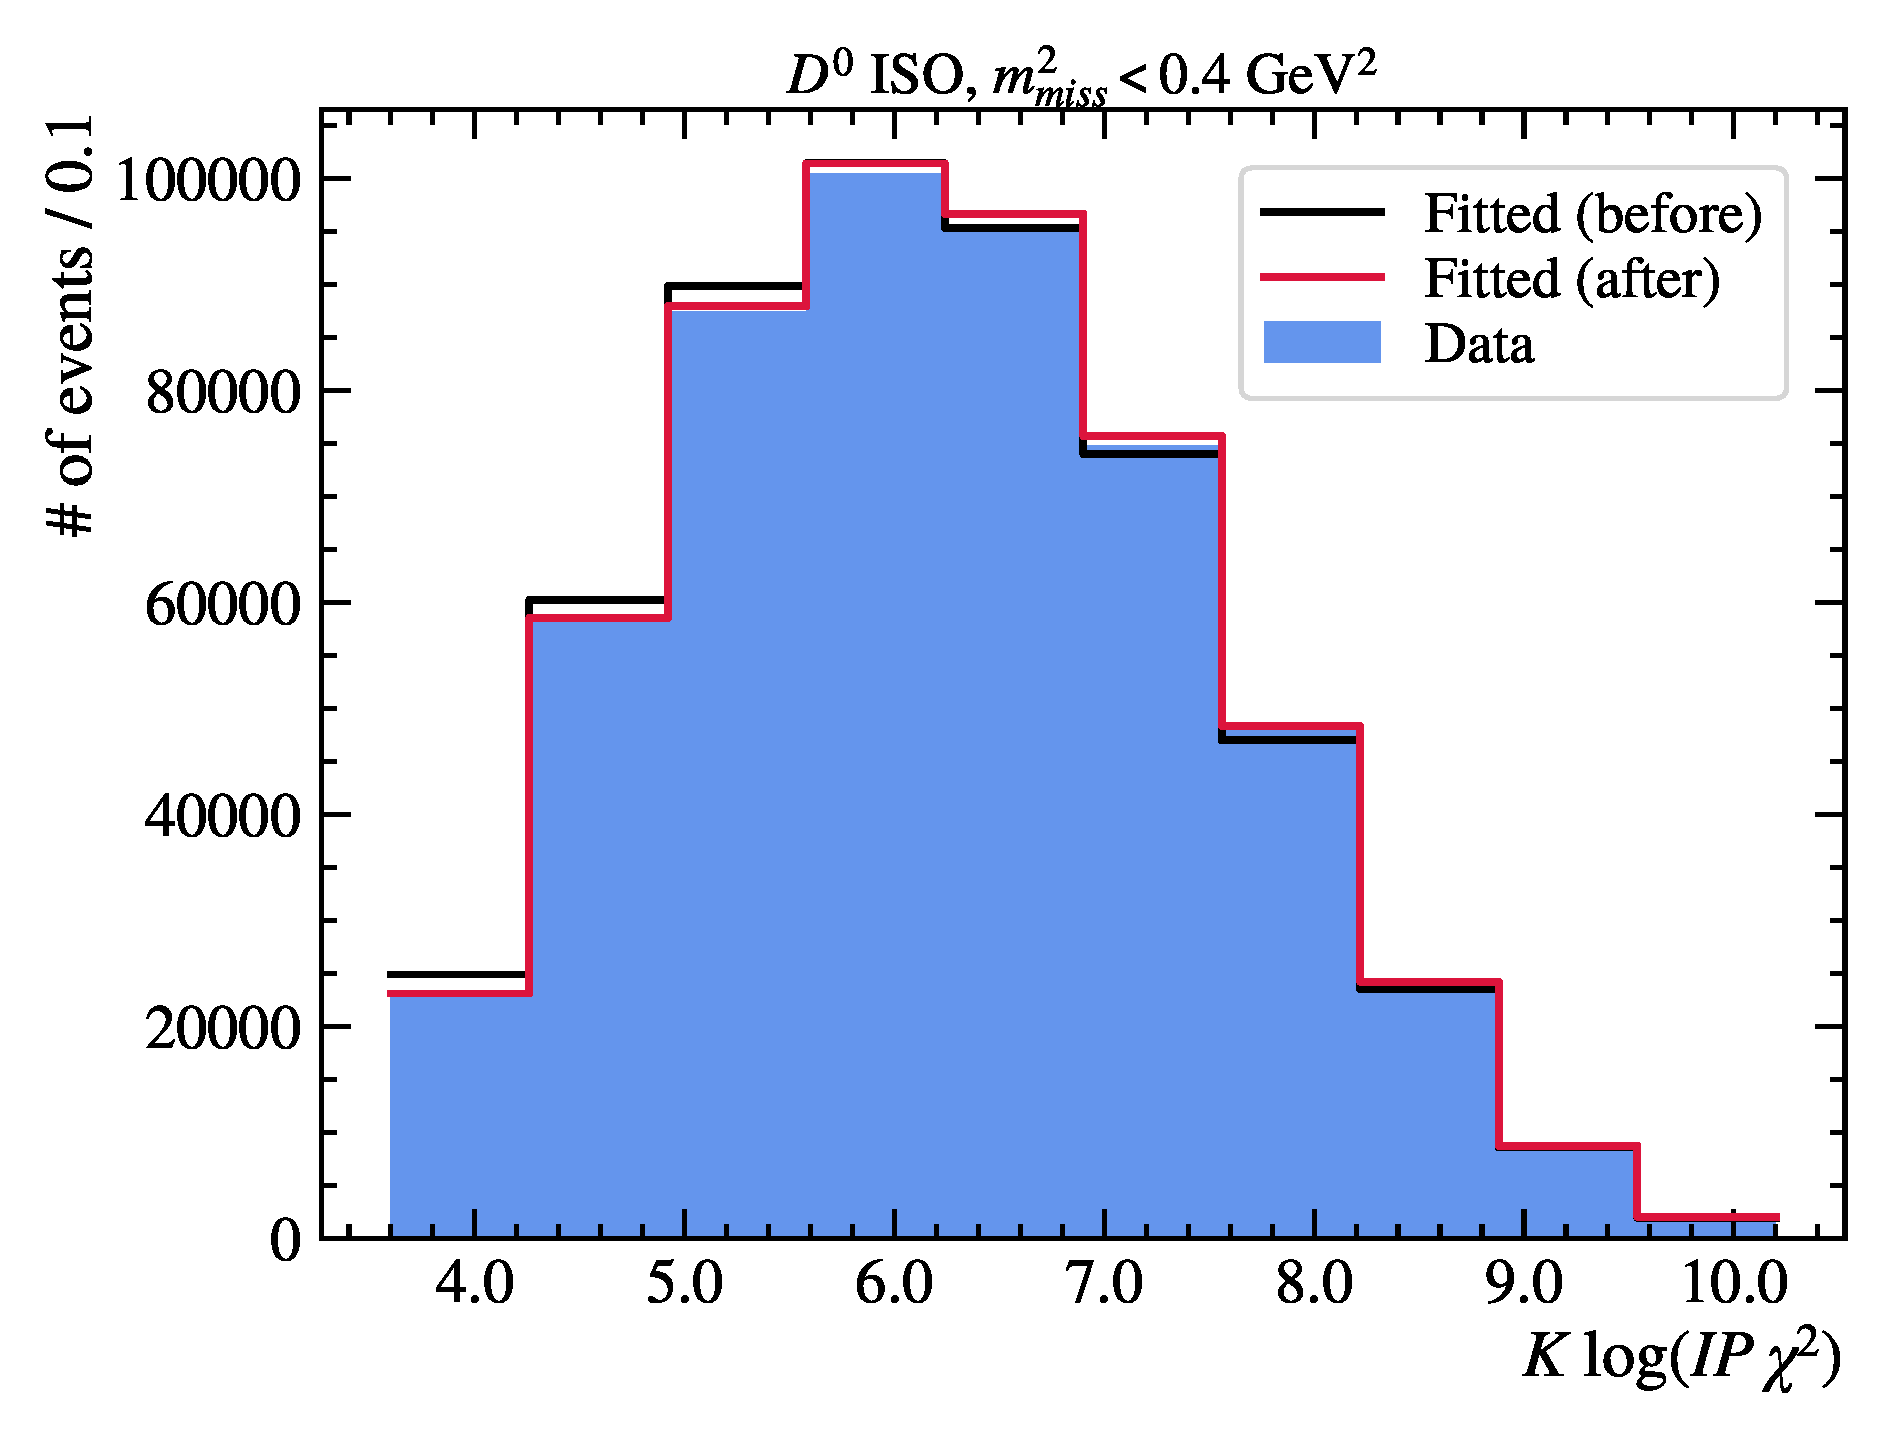
\includegraphics[width=0.32\textwidth]{./figs-mc-correction/reweighting-final/plot_step2-D0_iso-k_log_ip_chi2.pdf}
        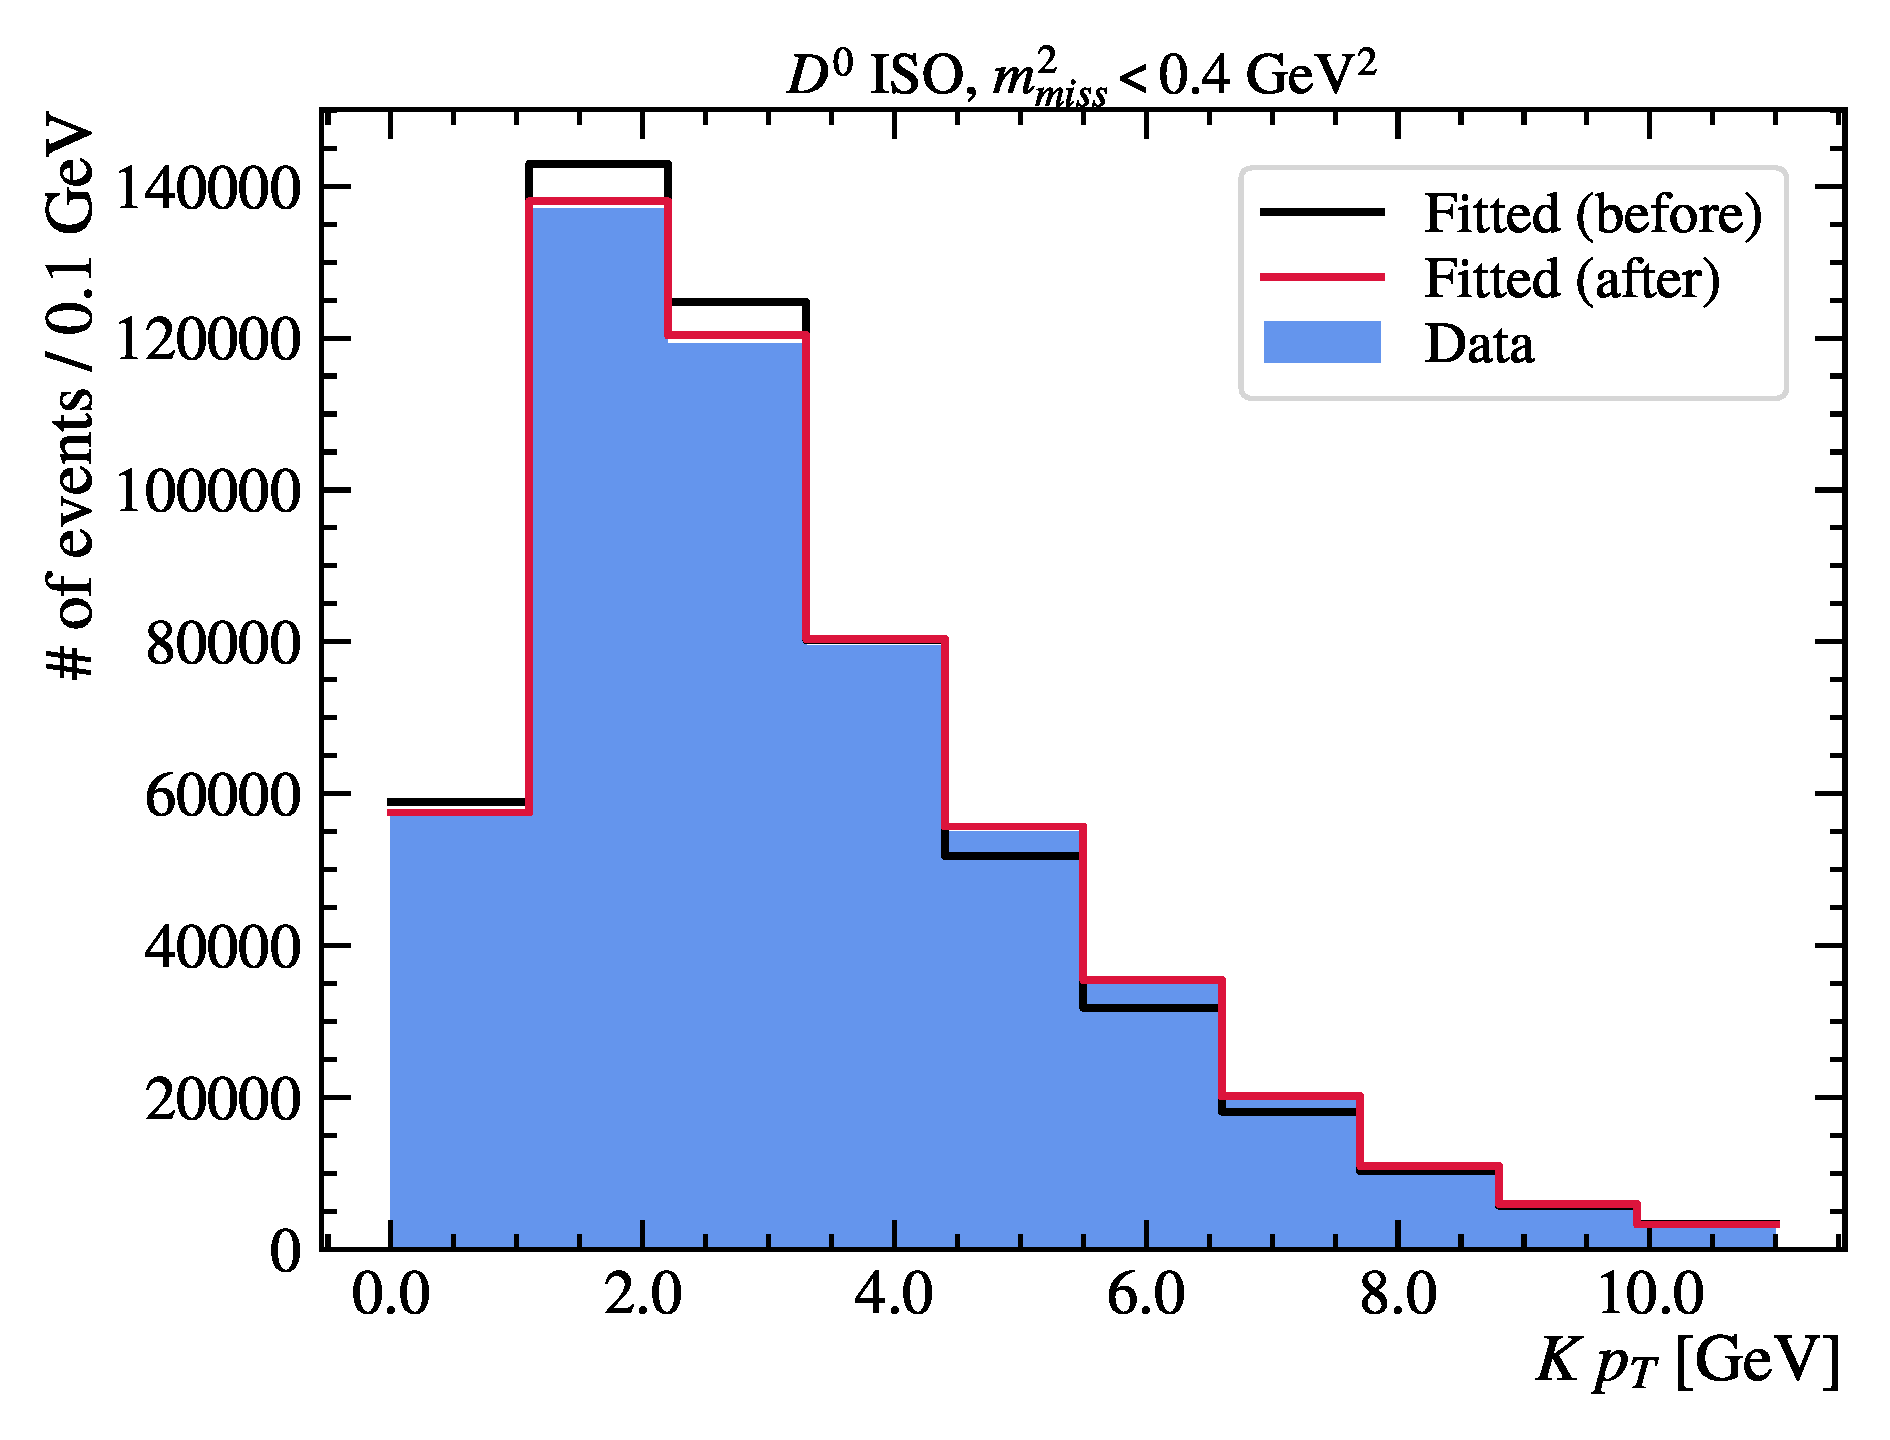
\includegraphics[width=0.32\textwidth]{./figs-mc-correction/reweighting-final/plot_step2-D0_iso-k_pt.pdf}
        \caption{Stage 3.}
    \end{subfigure}

    \begin{subfigure}{\textwidth}
        \centering
        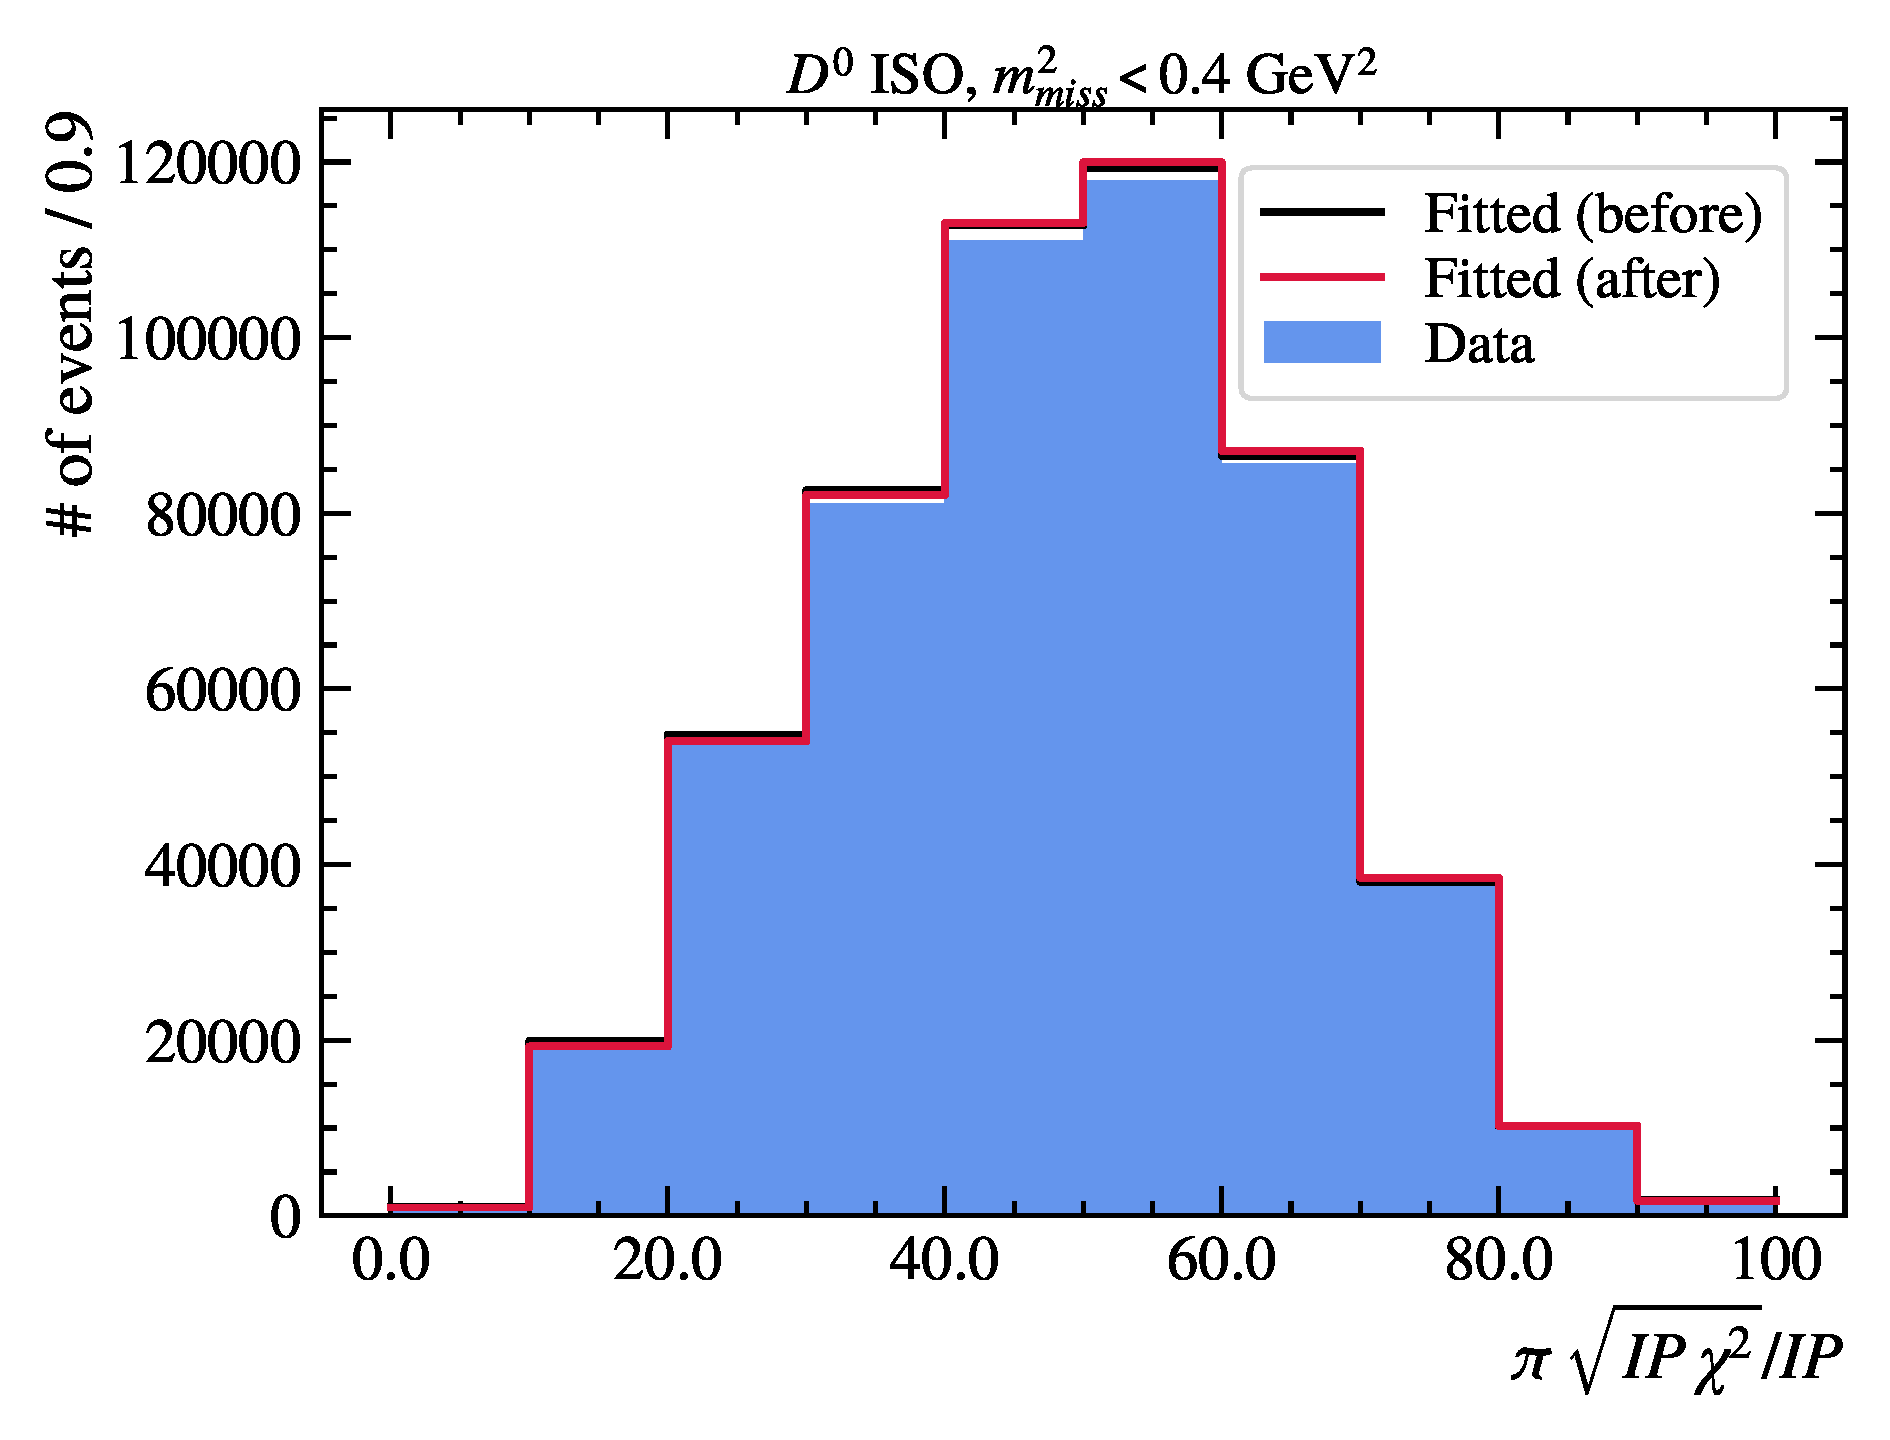
\includegraphics[width=0.32\textwidth]{./figs-mc-correction/reweighting-final/plot_step3-D0_iso-pi_comp.pdf}
        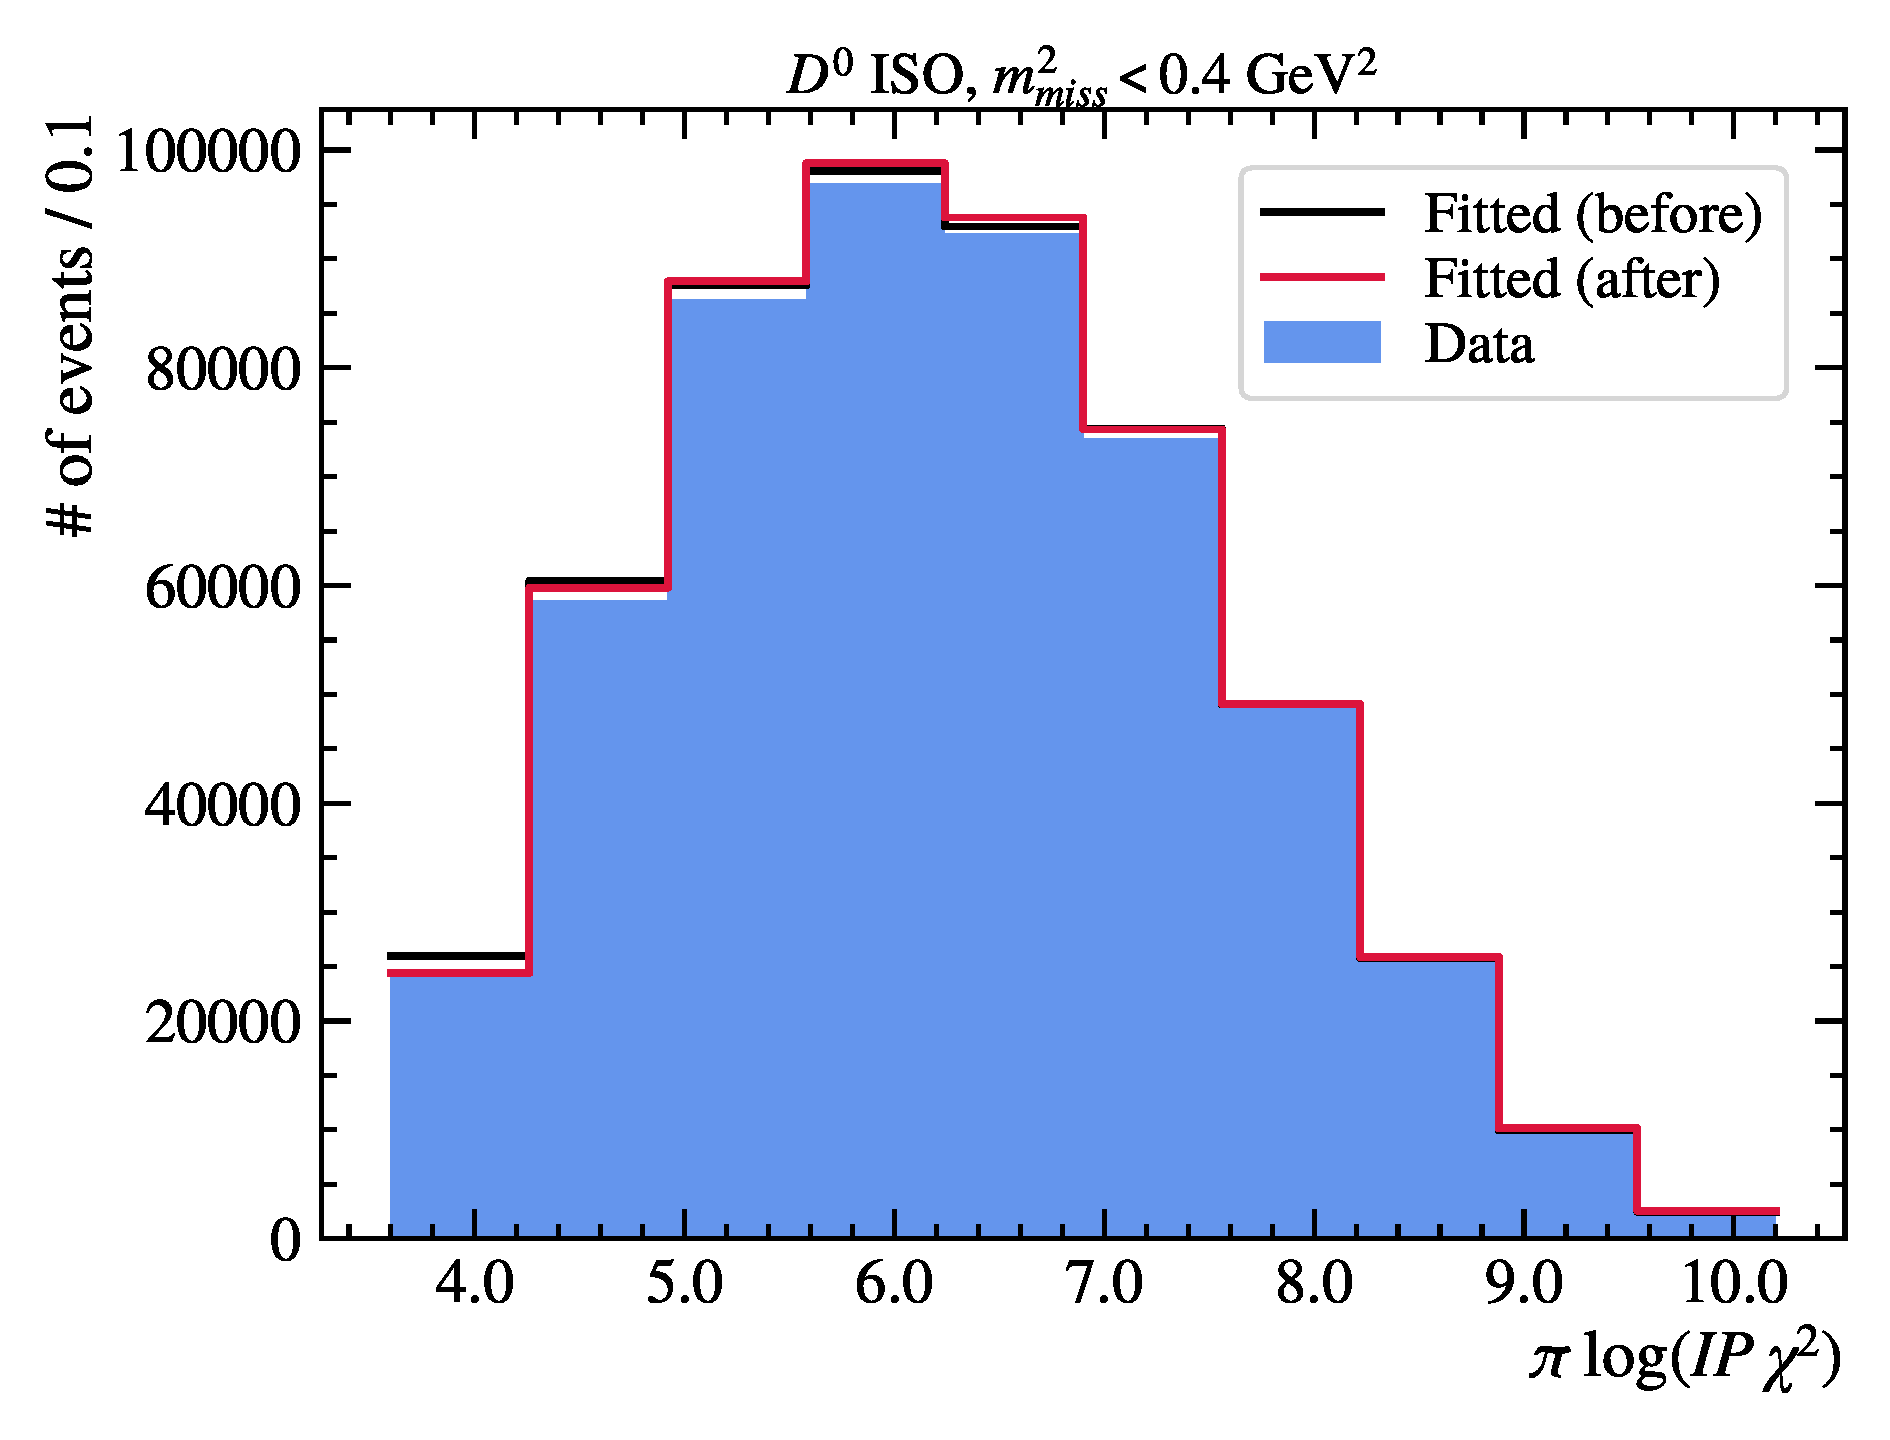
\includegraphics[width=0.32\textwidth]{./figs-mc-correction/reweighting-final/plot_step3-D0_iso-pi_log_ip_chi2.pdf}
        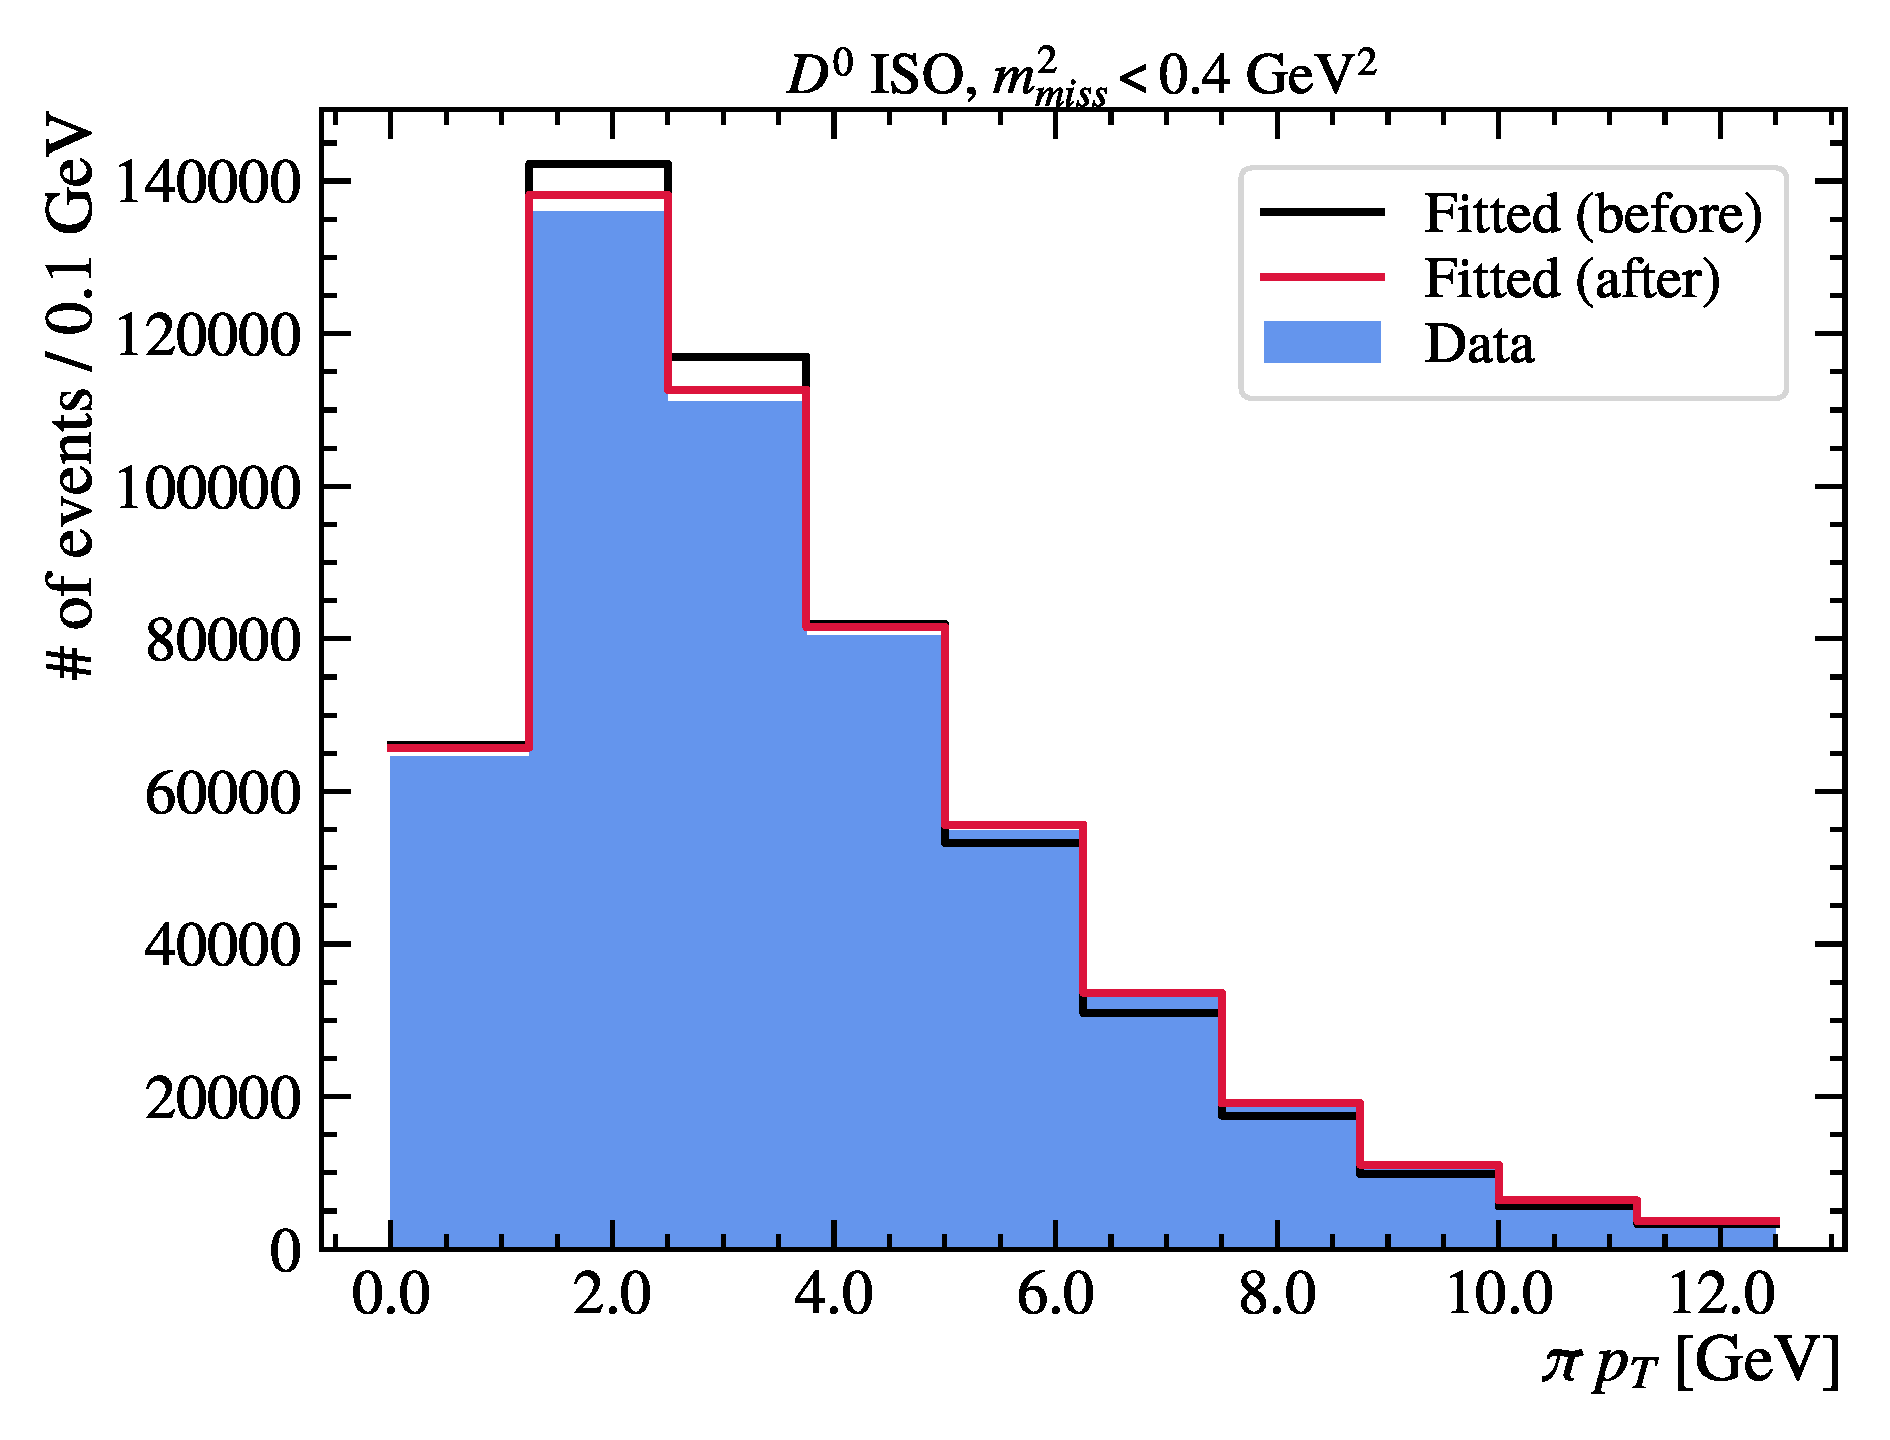
\includegraphics[width=0.32\textwidth]{./figs-mc-correction/reweighting-final/plot_step3-D0_iso-pi_pt.pdf}
        \caption{Stage 4.}
    \end{subfigure}

    \begin{subfigure}{\textwidth}
        \centering
        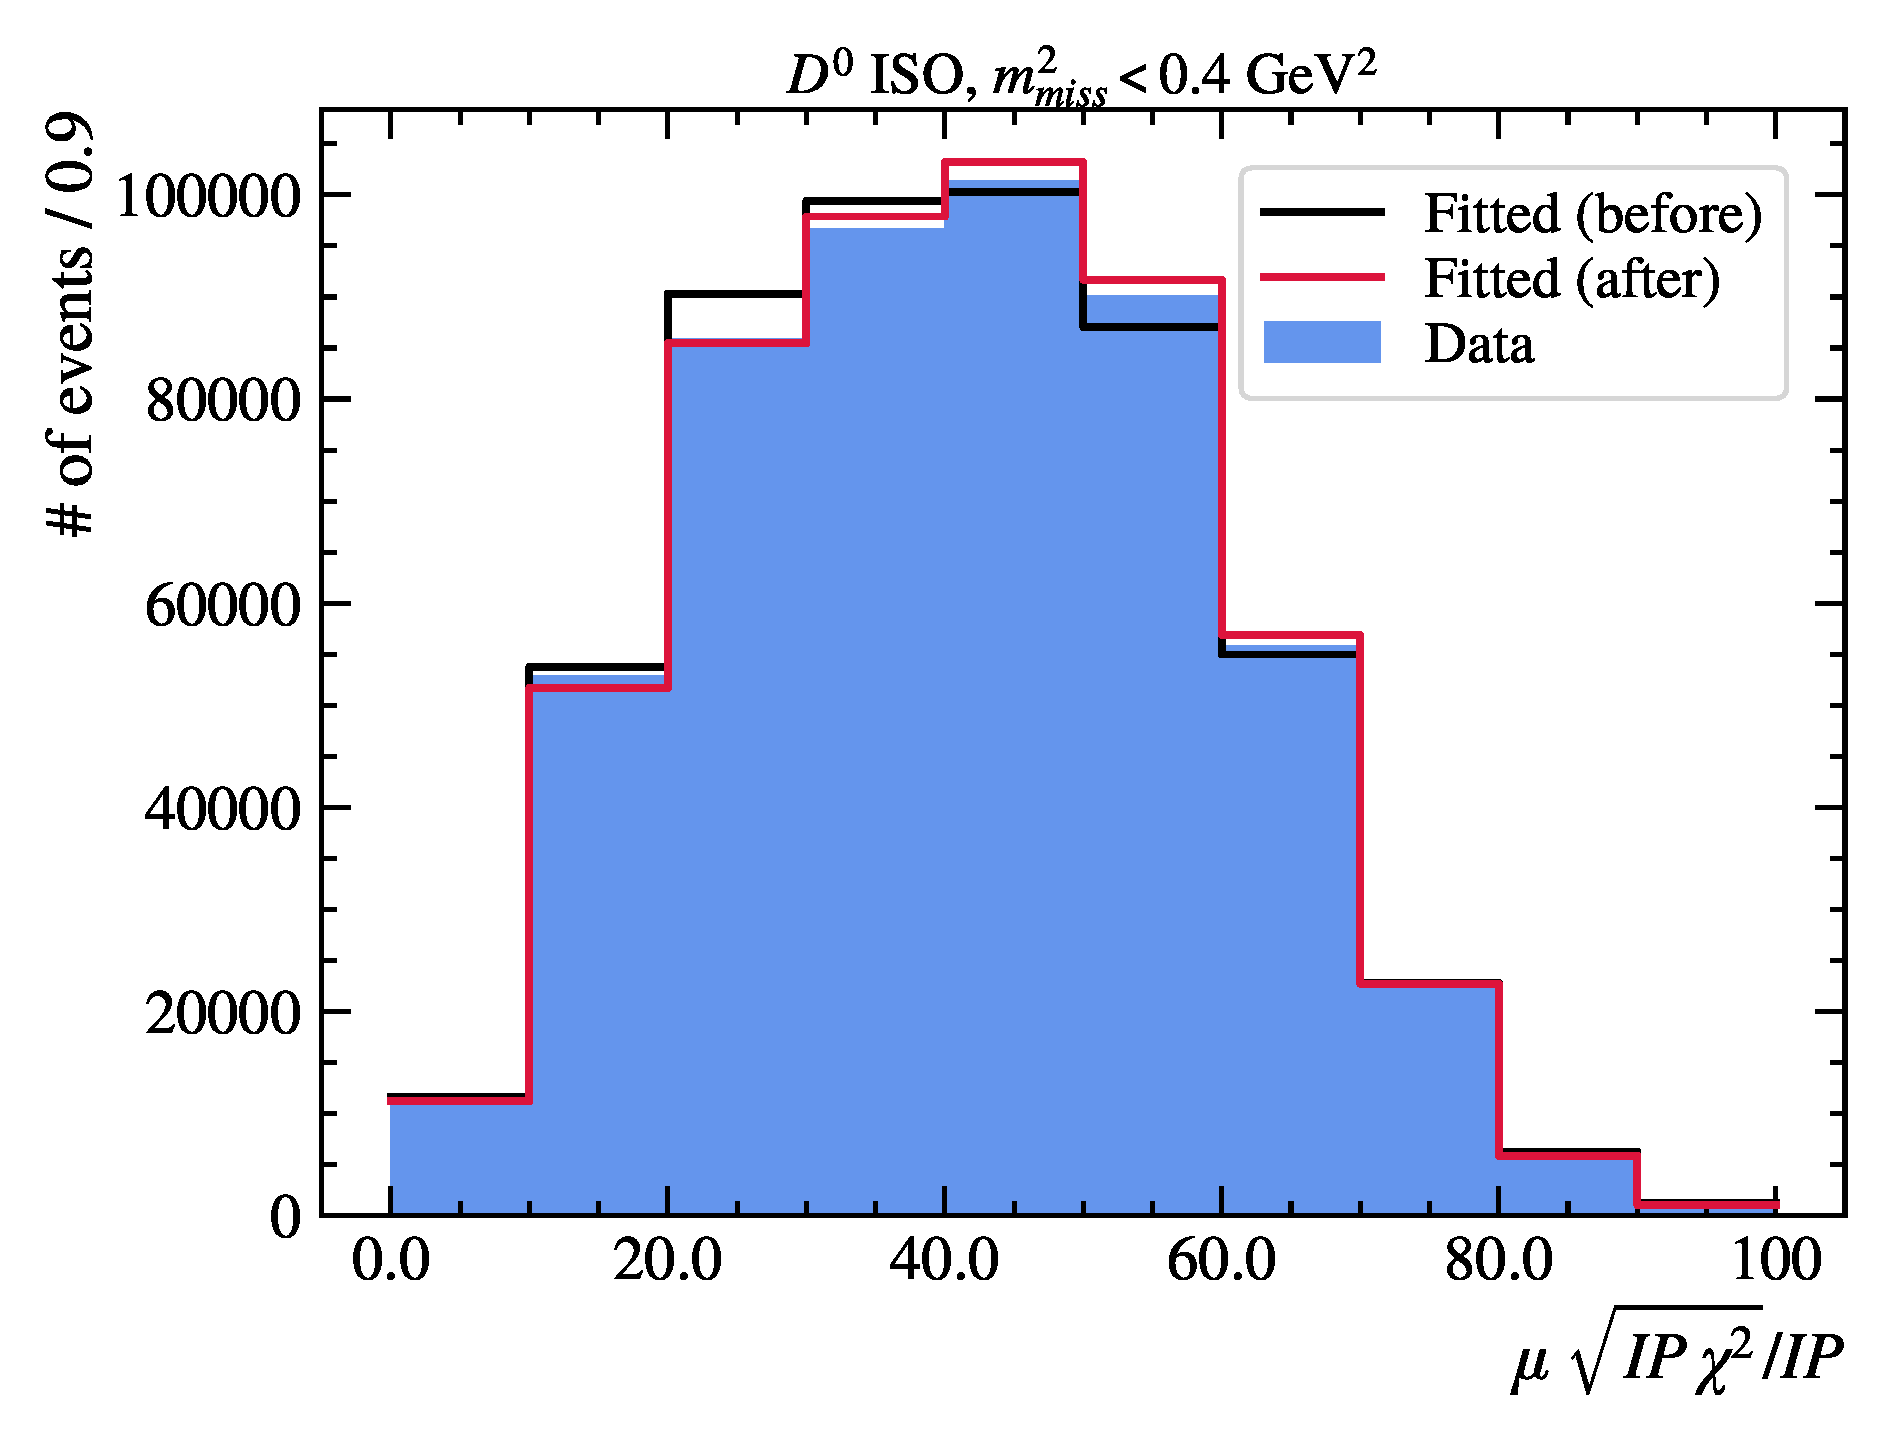
\includegraphics[width=0.32\textwidth]{./figs-mc-correction/reweighting-final/plot_step4-D0_iso-mu_comp.pdf}
        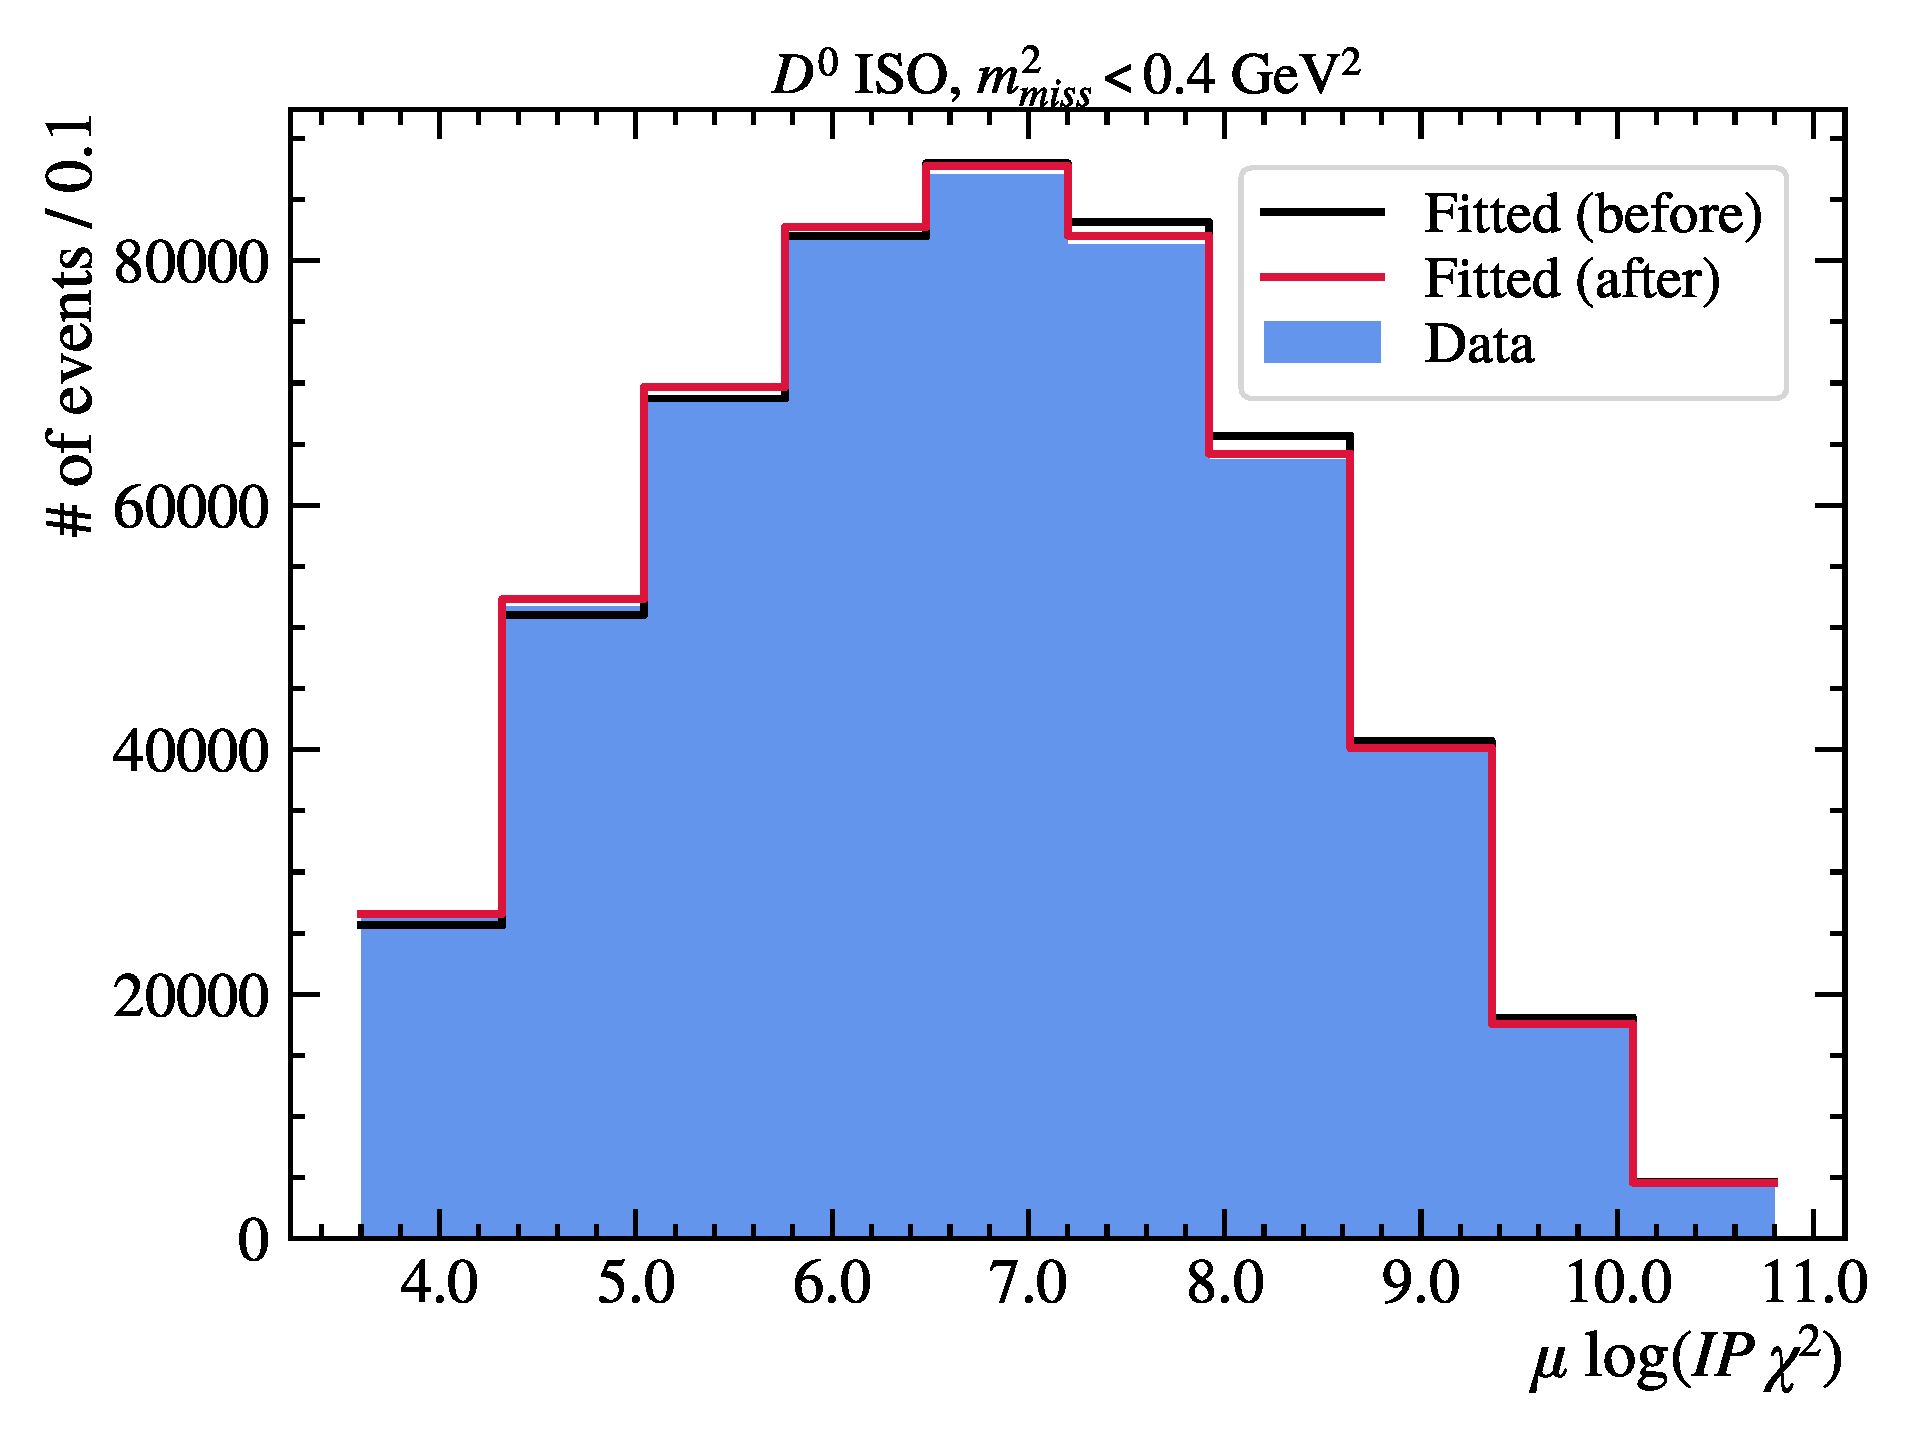
\includegraphics[width=0.32\textwidth]{./figs-mc-correction/reweighting-final/plot_step4-D0_iso-mu_log_ip_chi2.pdf}
        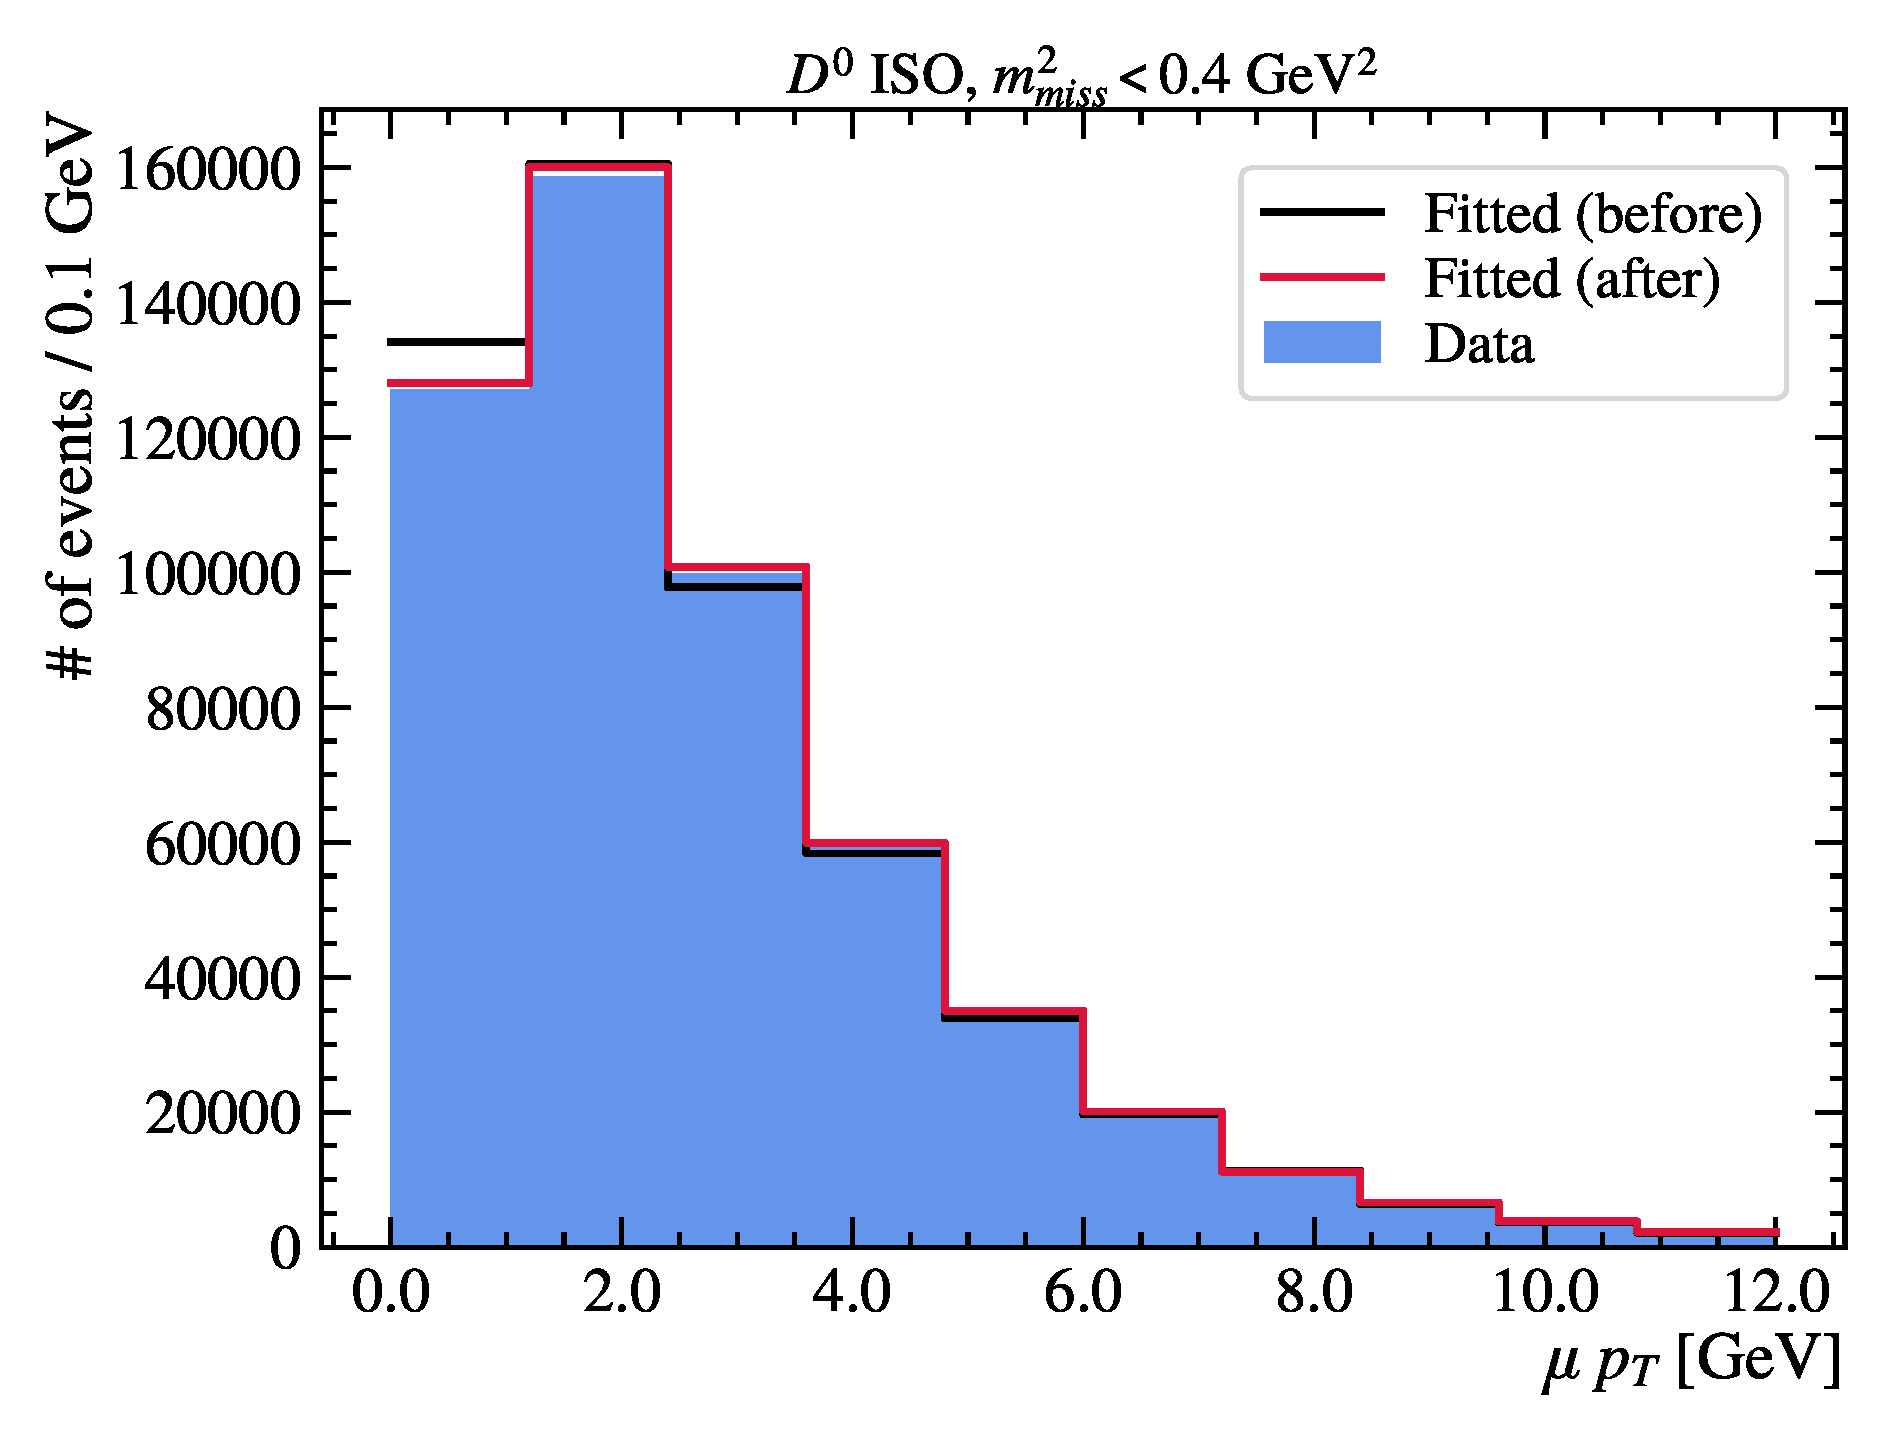
\includegraphics[width=0.32\textwidth]{./figs-mc-correction/reweighting-final/plot_step4-D0_iso-mu_pt.pdf}
        \caption{Stage 5.}
    \end{subfigure}

    \caption{Final reweighting for \Dz channel, stages 2--5 (cont'd).}
    \label{fig:final-rwt-d0-idx1}
\end{figure}

\begin{figure}[htb]
    \begin{subfigure}{\textwidth}
        \centering
        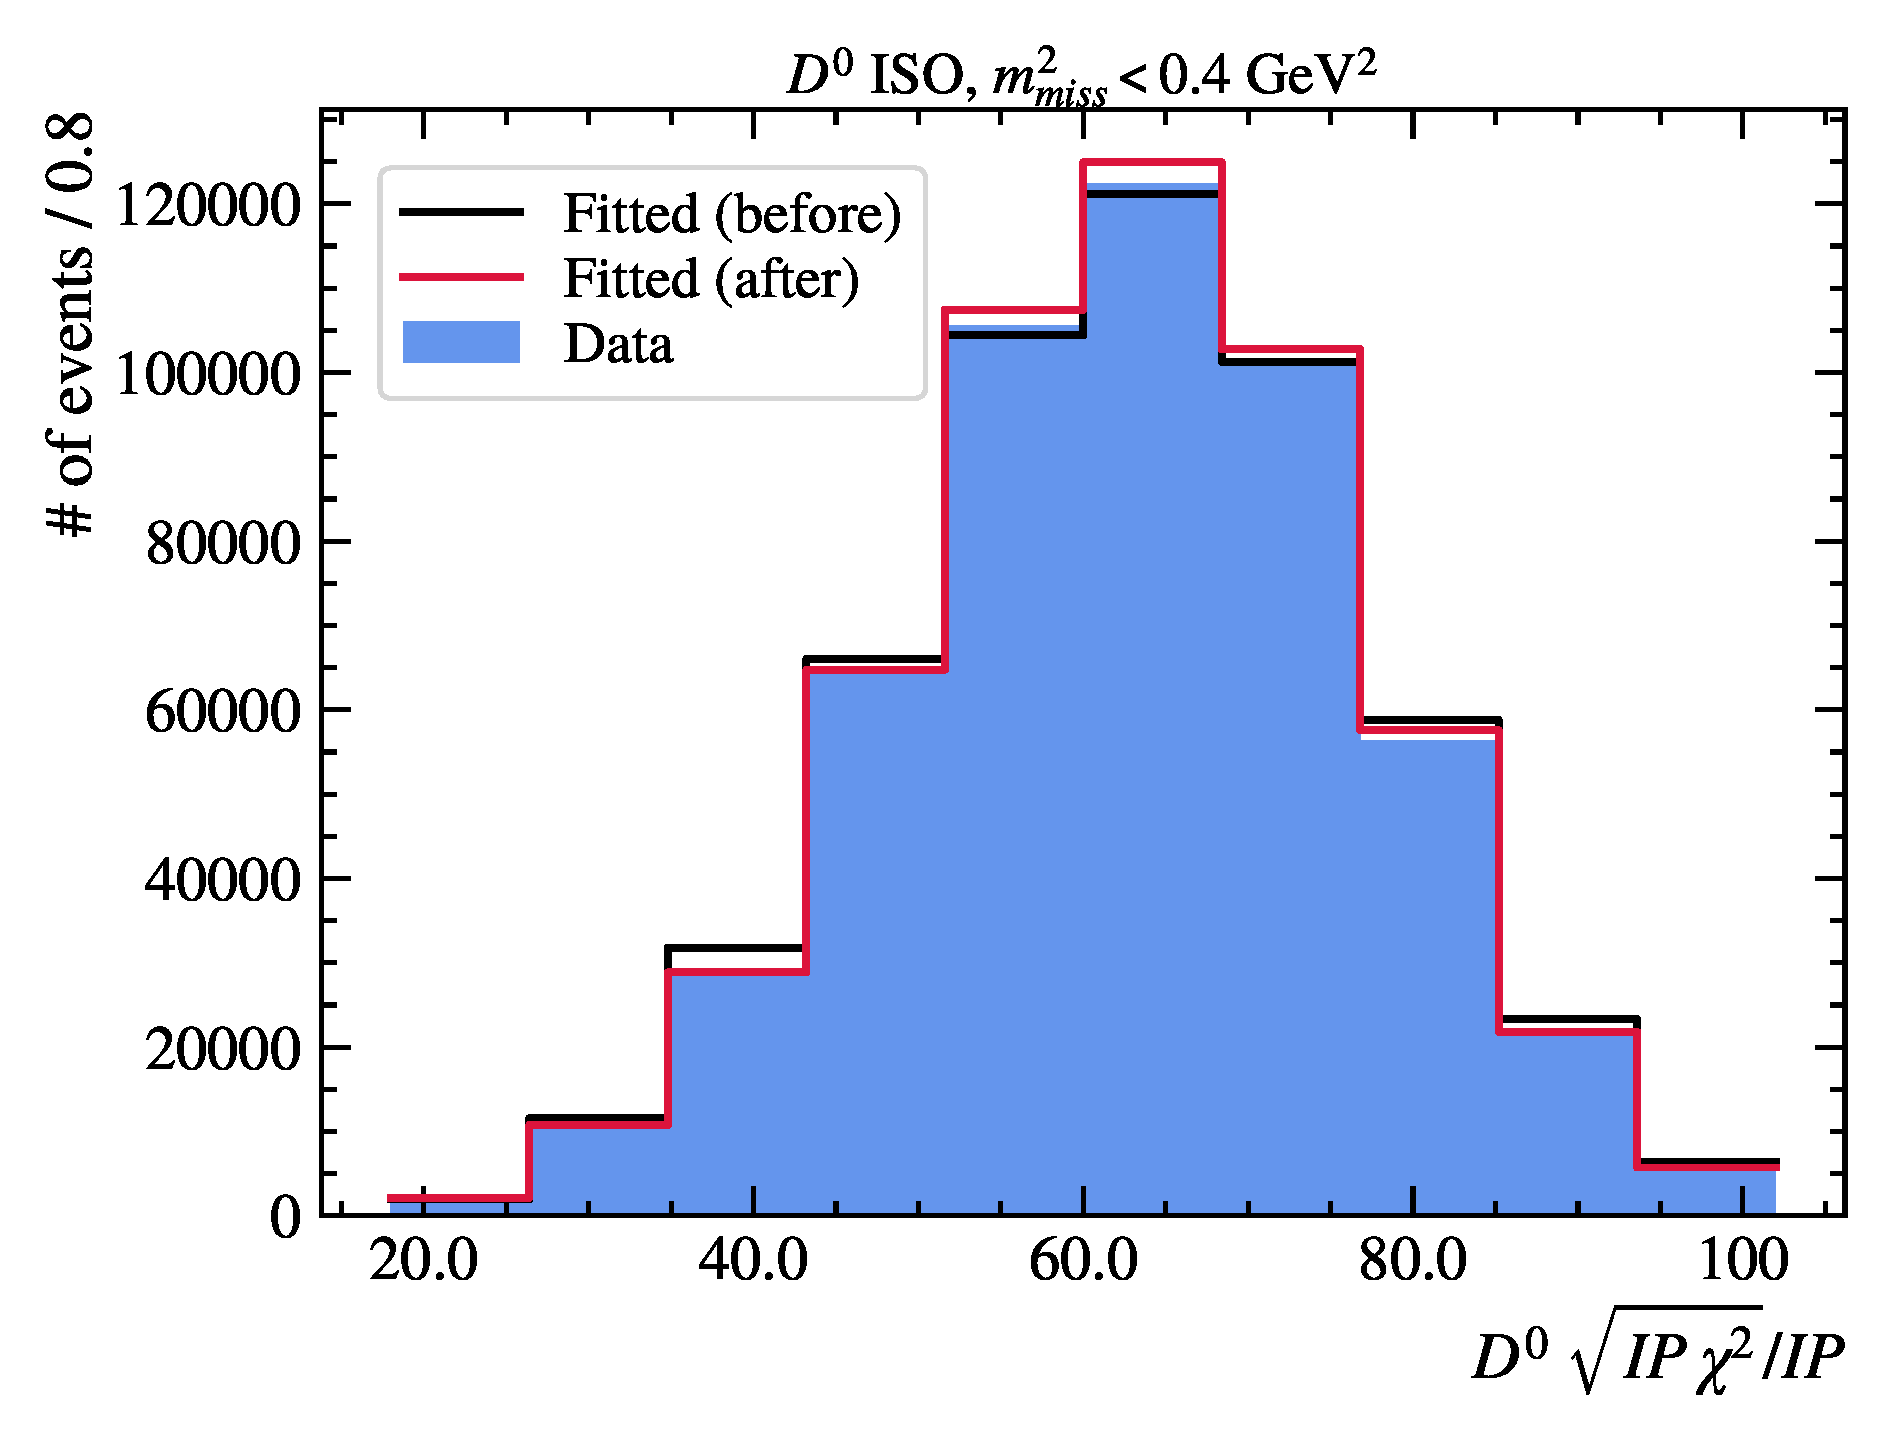
\includegraphics[width=0.32\textwidth]{./figs-mc-correction/reweighting-final/plot_step5-D0_iso-d0_comp.pdf}
        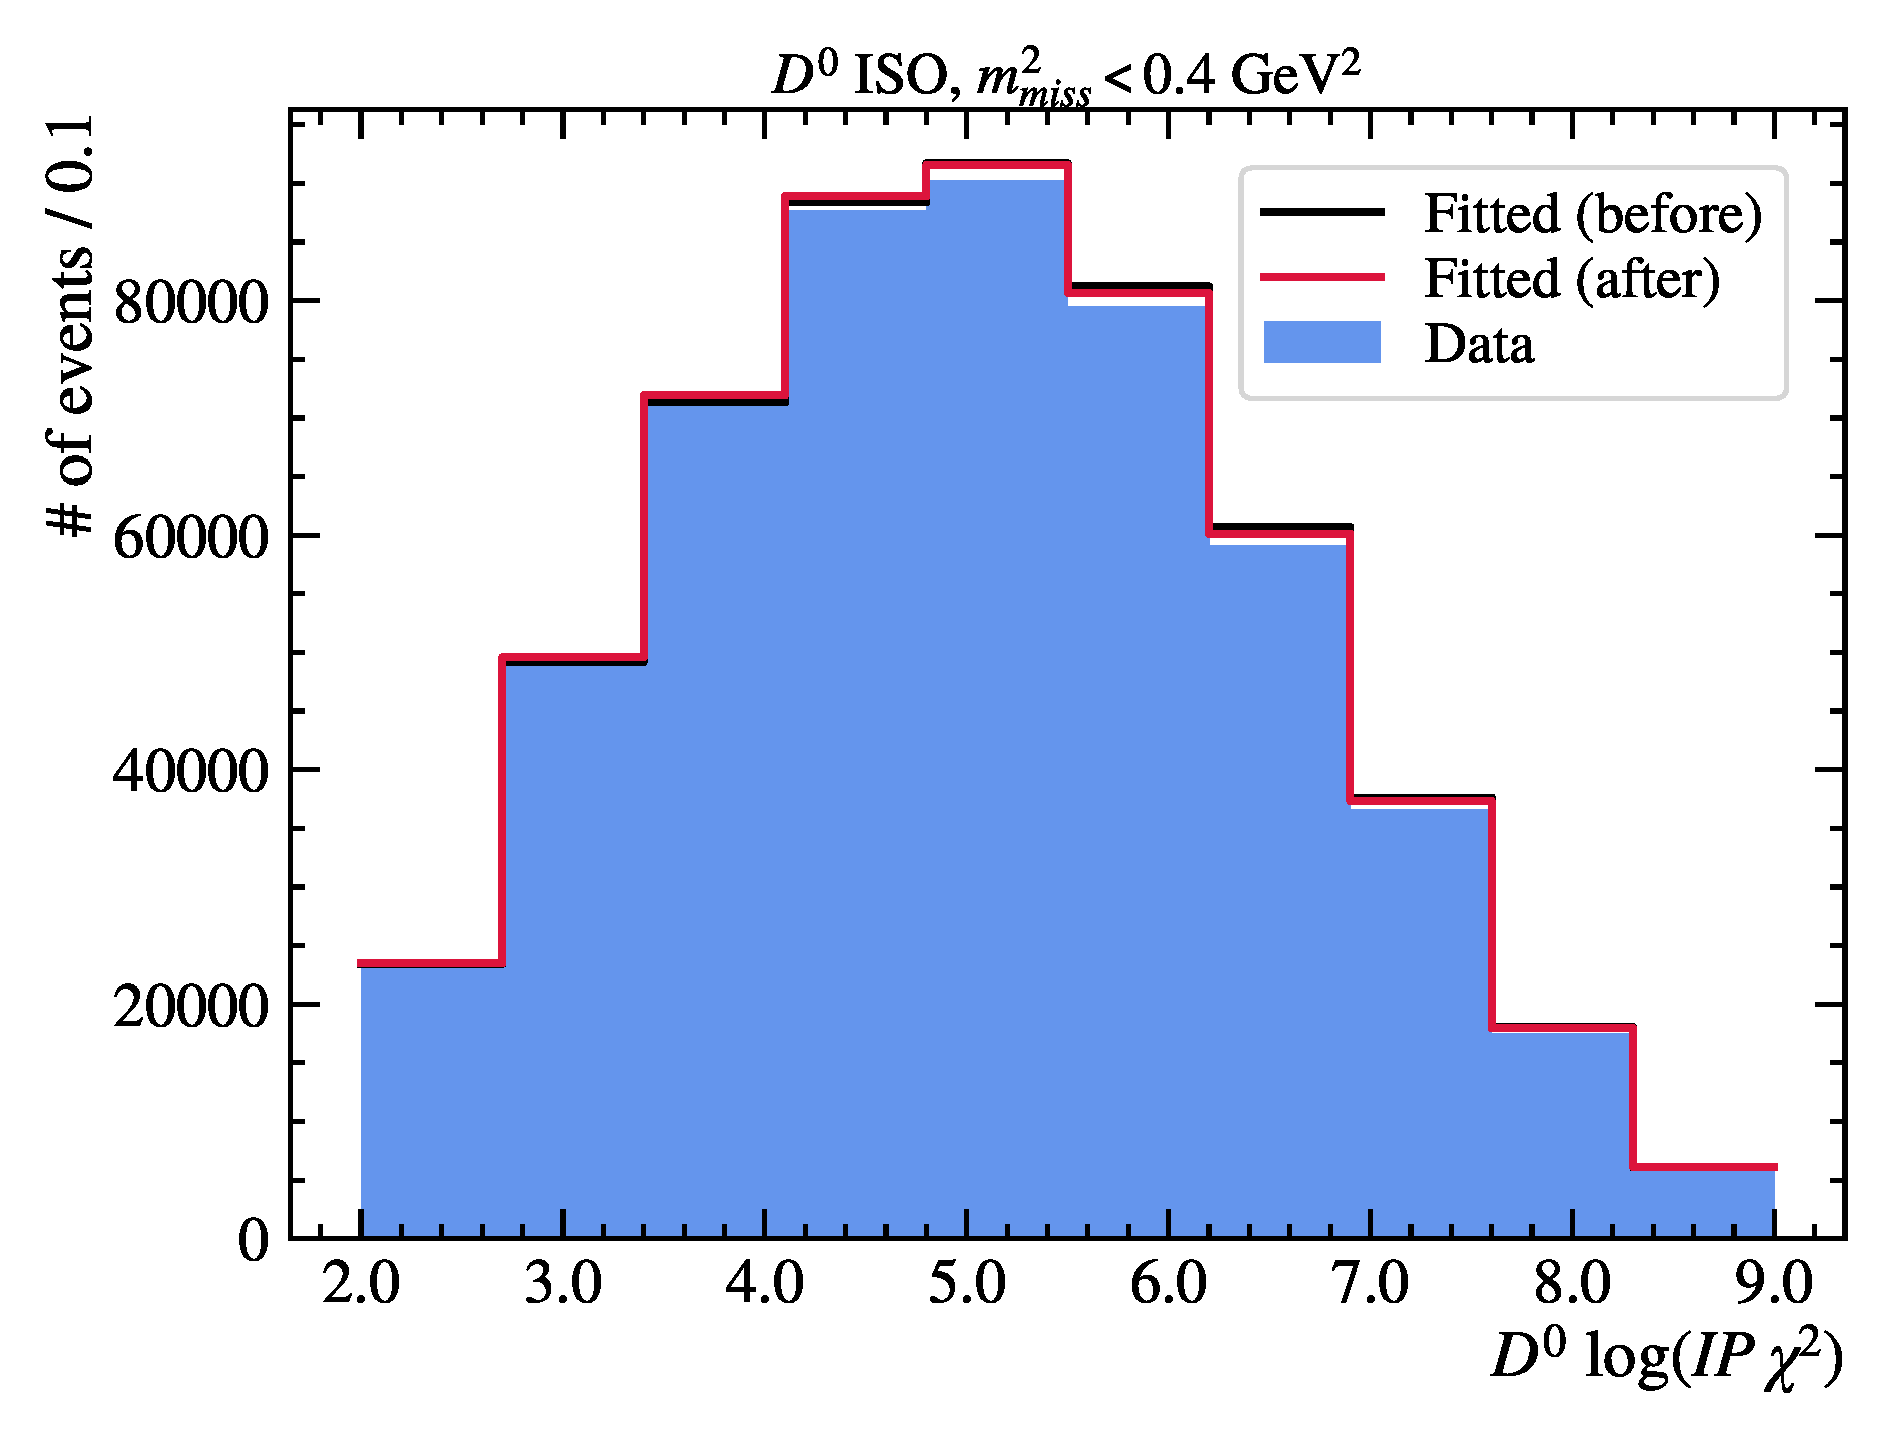
\includegraphics[width=0.32\textwidth]{./figs-mc-correction/reweighting-final/plot_step5-D0_iso-d0_log_ip_chi2.pdf}
        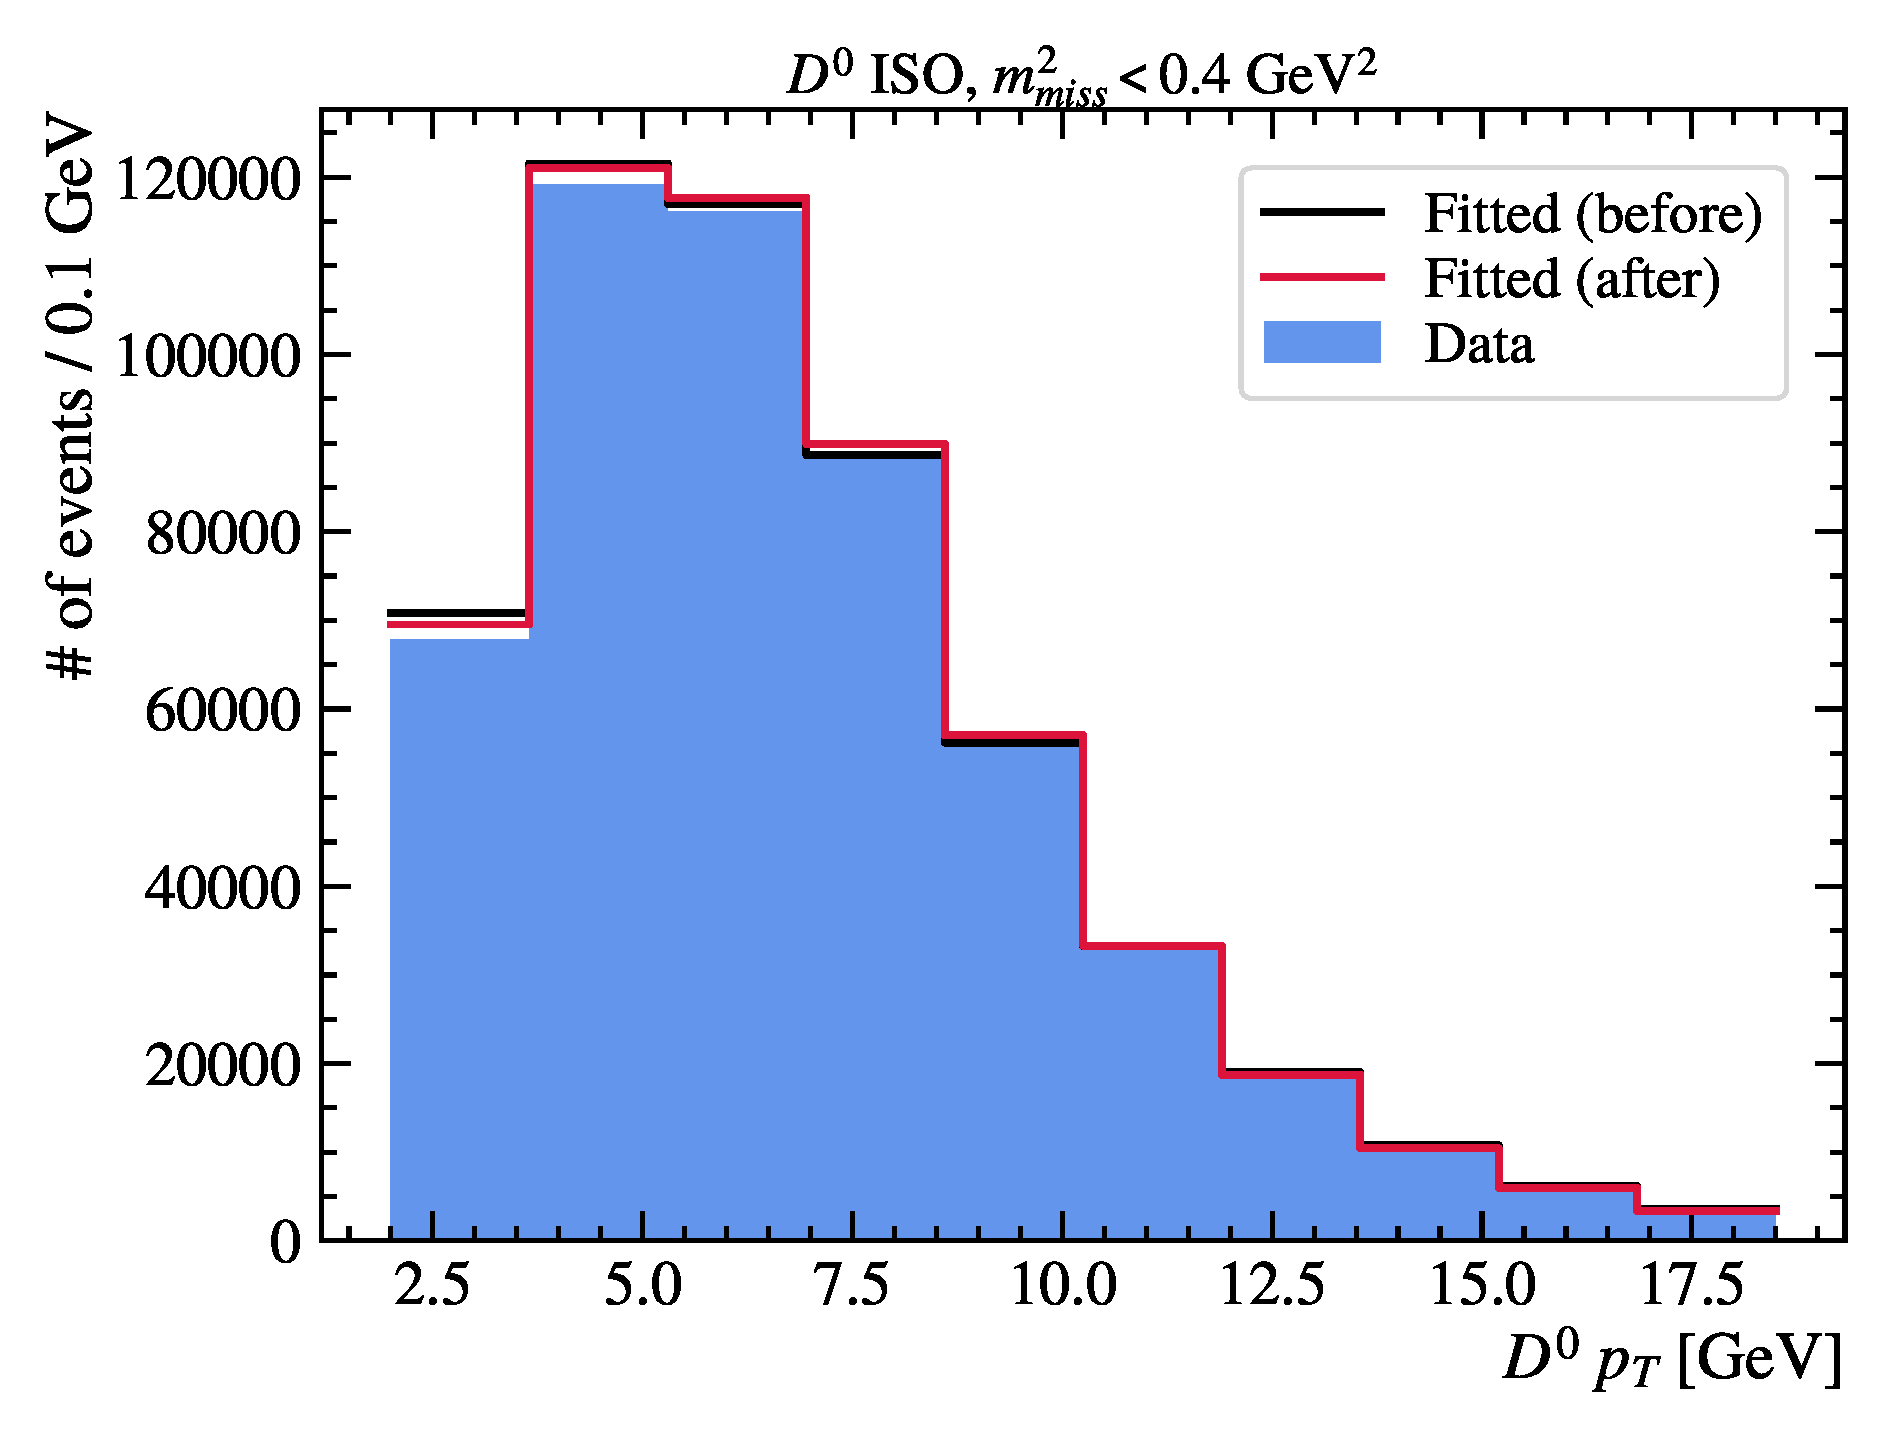
\includegraphics[width=0.32\textwidth]{./figs-mc-correction/reweighting-final/plot_step5-D0_iso-d0_pt.pdf}
        \caption{Stage 6.}
    \end{subfigure}

    \begin{subfigure}{\textwidth}
        \centering
        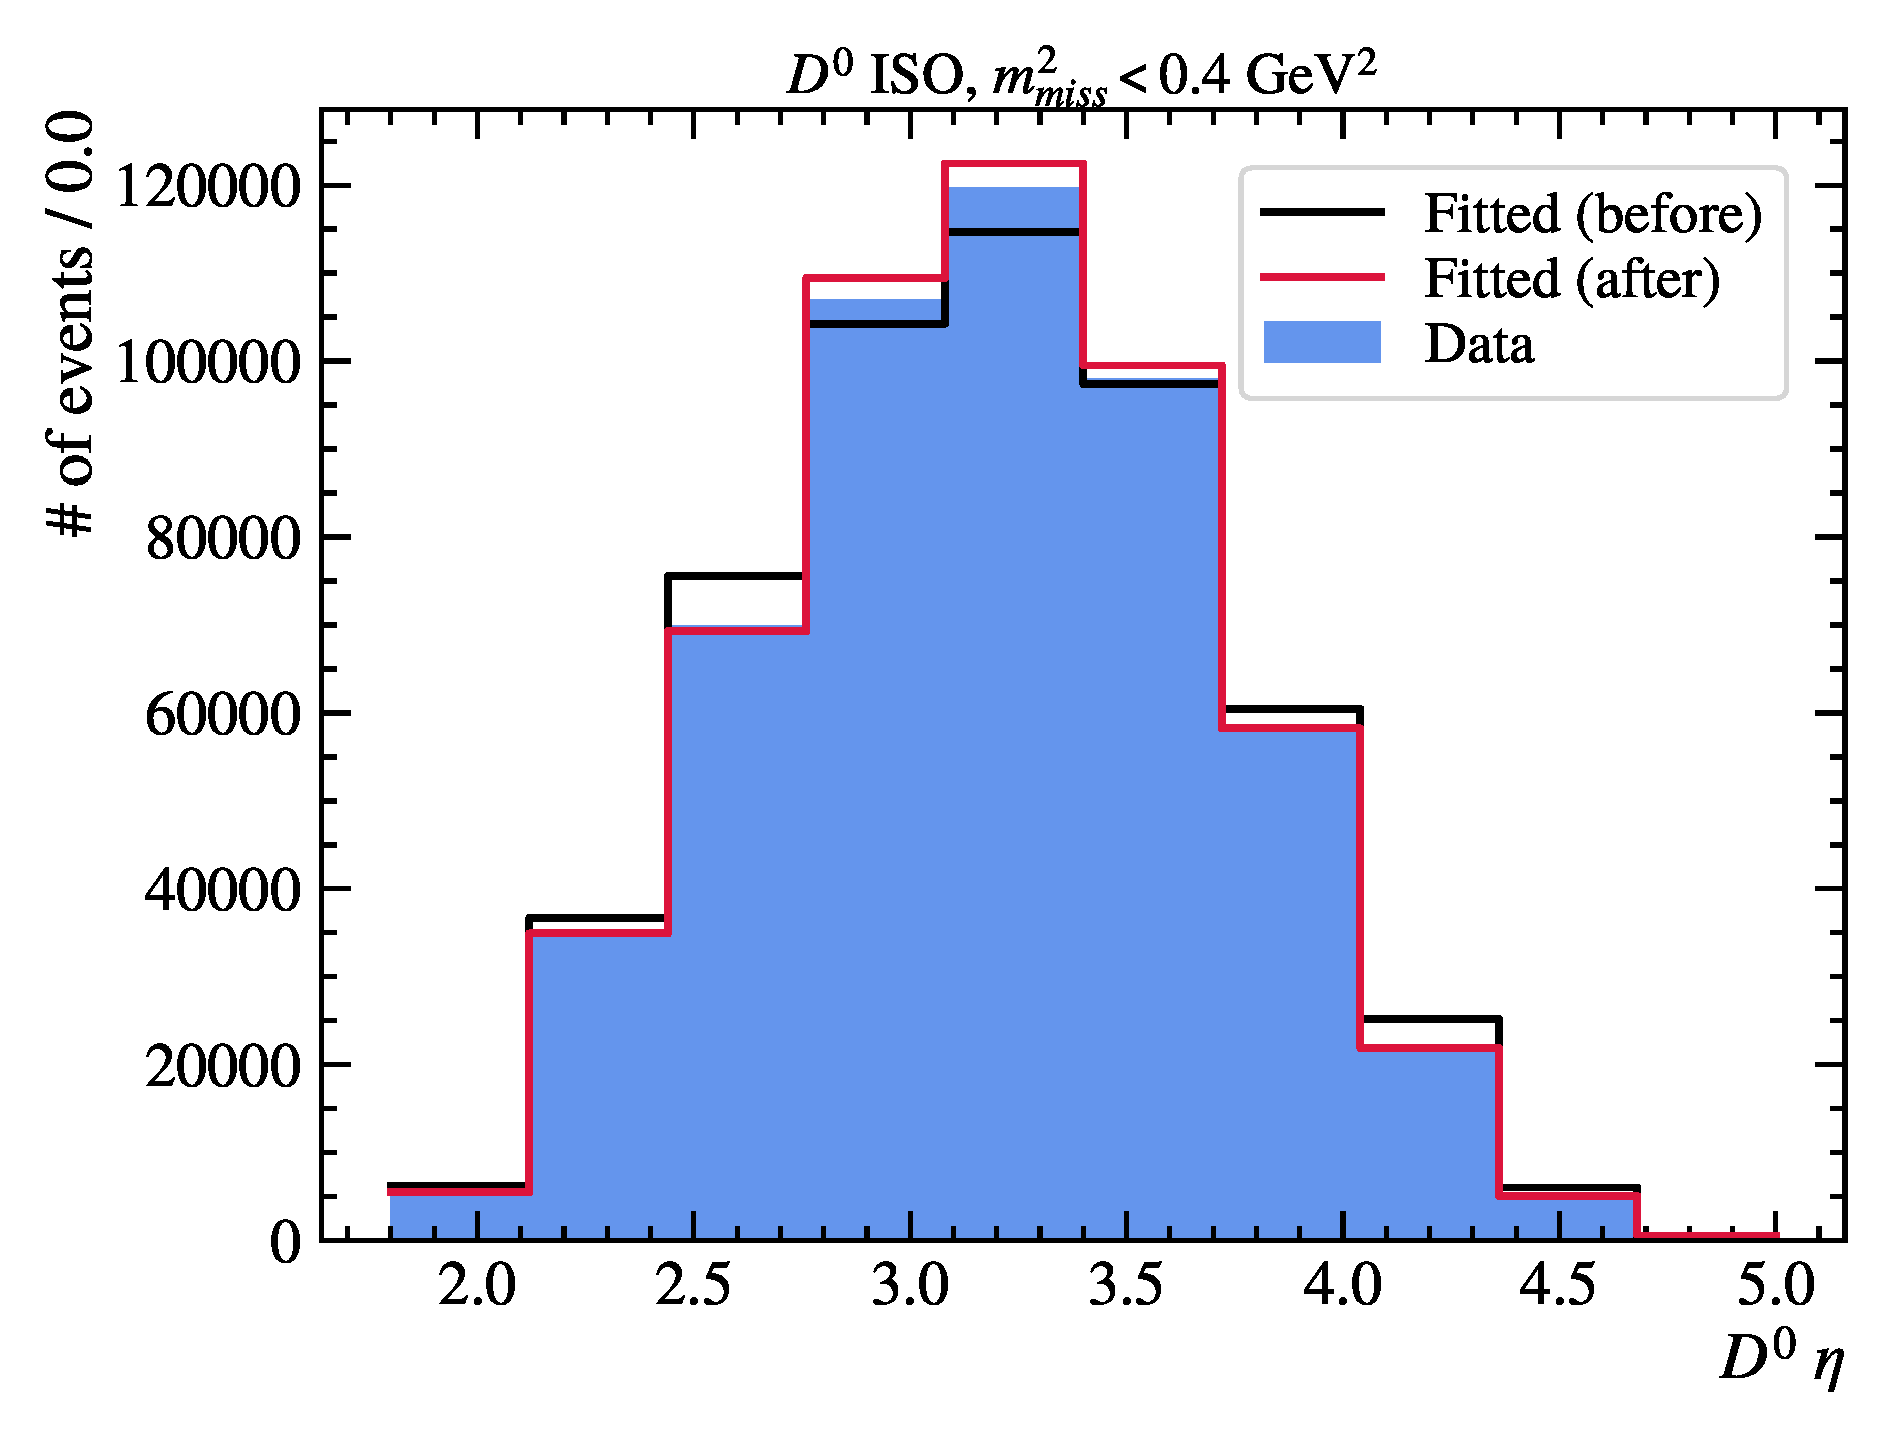
\includegraphics[width=0.32\textwidth]{./figs-mc-correction/reweighting-final/plot_step6-D0_iso-d0_eta.pdf}
        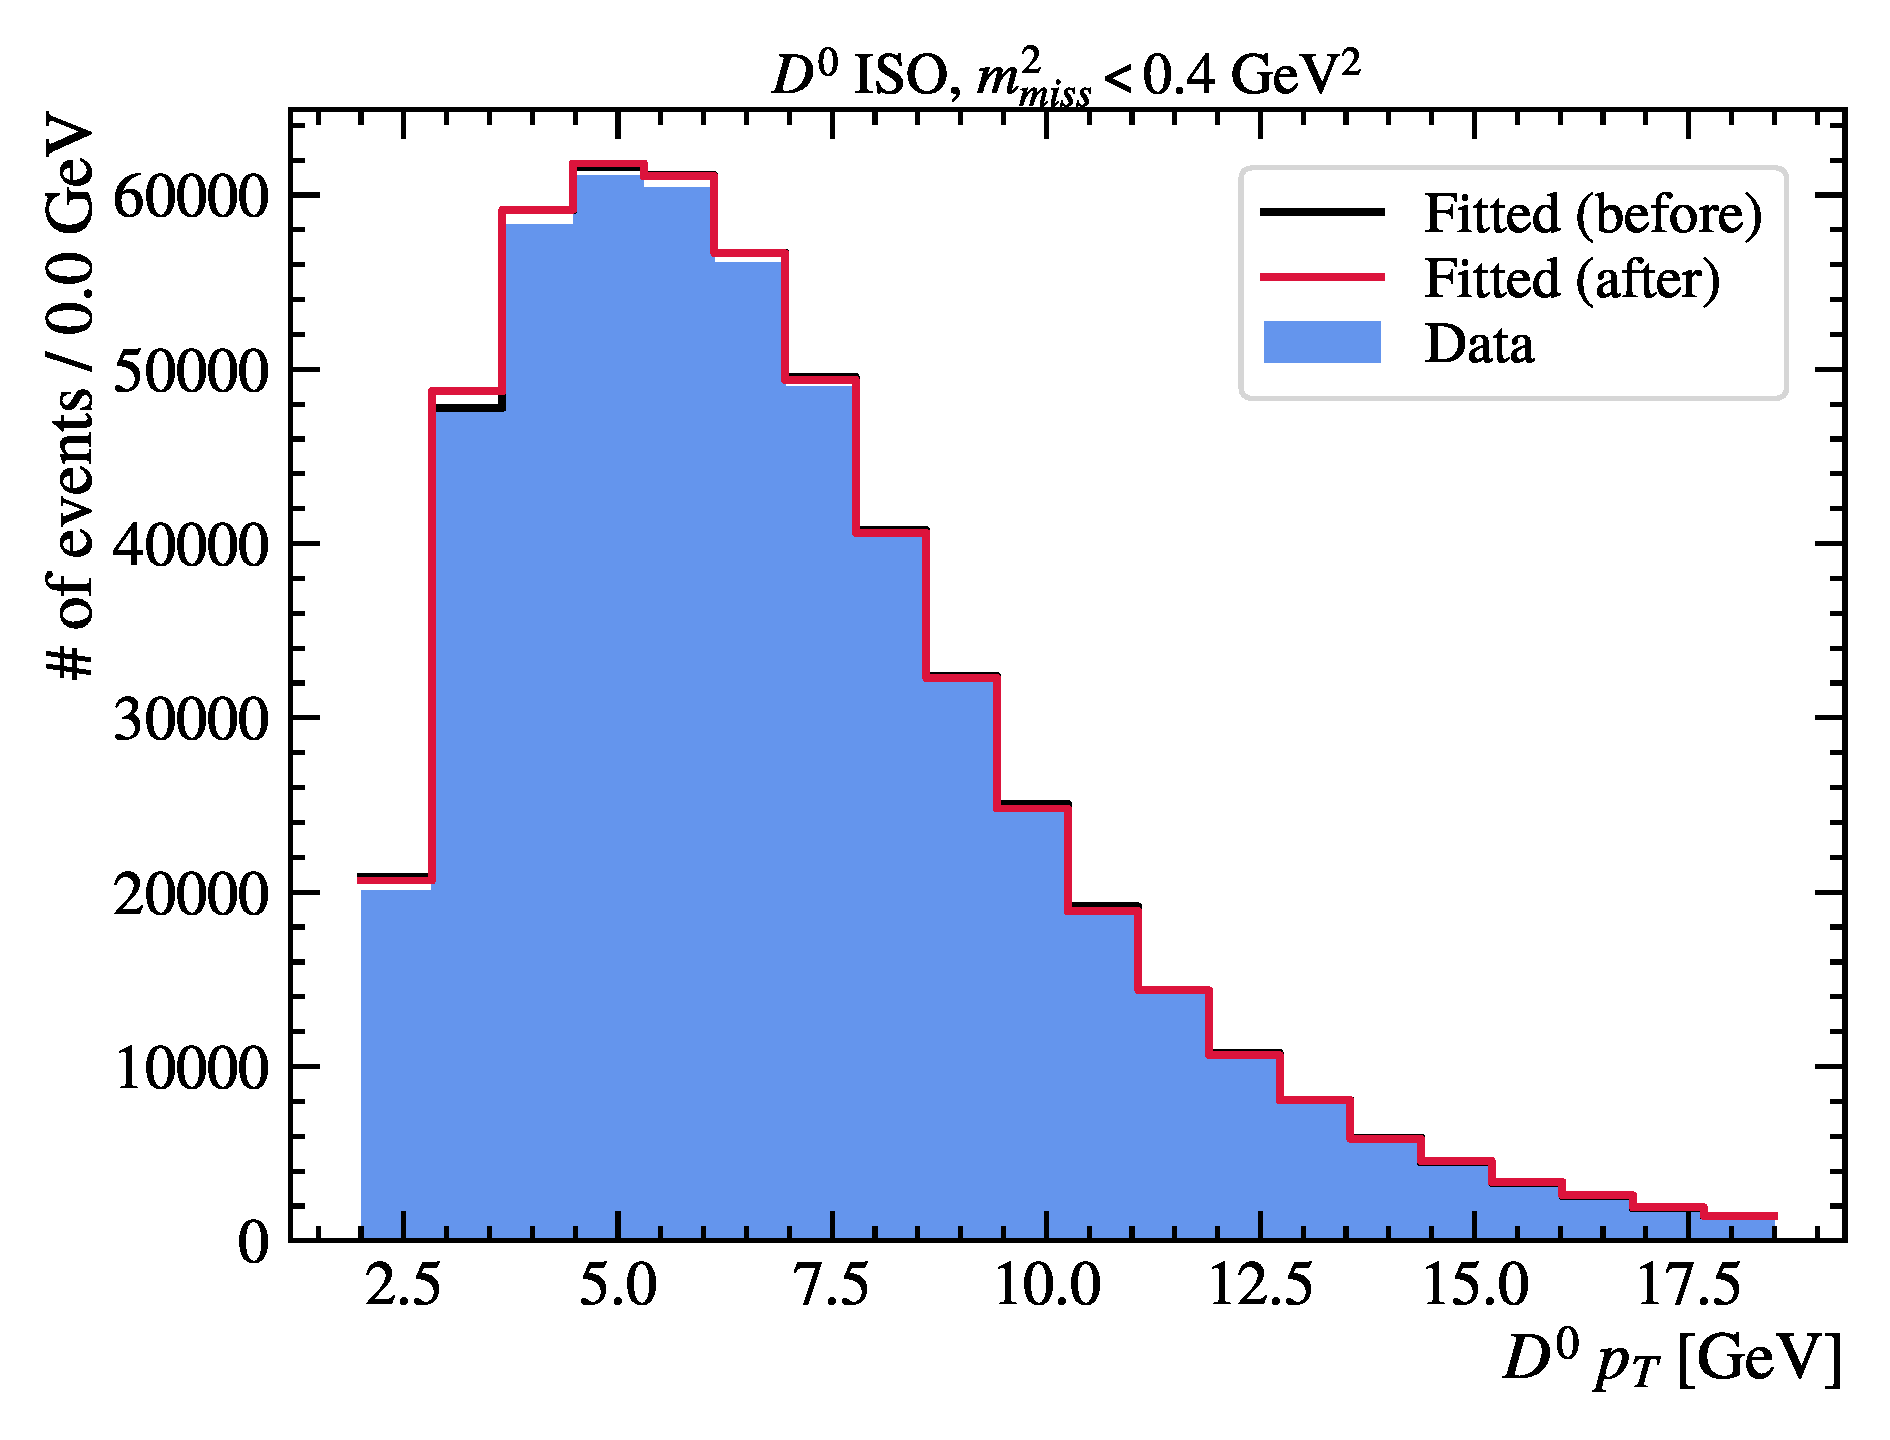
\includegraphics[width=0.32\textwidth]{./figs-mc-correction/reweighting-final/plot_step6-D0_iso-d0_pt.pdf}
        \caption{Stage 7.}
    \end{subfigure}

    \begin{subfigure}{\textwidth}
        \centering
        \includegraphics[width=0.32\textwidth]{./figs-mc-correction/reweighting-final/plot_step7-D0_iso-k_eta.pdf}
        \includegraphics[width=0.32\textwidth]{./figs-mc-correction/reweighting-final/plot_step7-D0_iso-k_pt.pdf}
        \caption{Stage 8.}
    \end{subfigure}

    \begin{subfigure}{\textwidth}
        \centering
        \includegraphics[width=0.32\textwidth]{./figs-mc-correction/reweighting-final/plot_step8-D0_iso-pi_eta.pdf}
        \includegraphics[width=0.32\textwidth]{./figs-mc-correction/reweighting-final/plot_step8-D0_iso-pi_pt.pdf}
        \caption{Stage 9.}
    \end{subfigure}

    \caption{Final reweighting for \Dz channel, stages 6--9 (cont'd).}
    \label{fig:final-rwt-d0-idx2}
\end{figure}

\begin{figure}[htb]
    \begin{subfigure}{\textwidth}
        \centering
        \includegraphics[width=0.32\textwidth]{./figs-mc-correction/reweighting-final/plot_step9-D0_iso-mu_eta.pdf}
        \includegraphics[width=0.32\textwidth]{./figs-mc-correction/reweighting-final/plot_step9-D0_iso-mu_pt.pdf}
        \caption{Stage 10.}
    \end{subfigure}

    \begin{subfigure}{\textwidth}
        \centering
        \includegraphics[width=0.32\textwidth]{./figs-mc-correction/reweighting-final/plot_step10-D0_iso-d0_comp2.pdf}
        \caption{Stage 11.}
    \end{subfigure}

    \caption{Final reweighting for \Dz channel, stages 10--11 (cont'd).}
    \label{fig:final-rwt-d0-idx3}
\end{figure}

%%%%
%%%%

\begin{figure}[htb]
    \begin{subfigure}{\textwidth}
        \centering
        \includegraphics[width=0.32\textwidth]{./figs-mc-correction/reweighting-final/plot_step0-Dst_iso-k_comp.pdf}
        \includegraphics[width=0.32\textwidth]{./figs-mc-correction/reweighting-final/plot_step0-Dst_iso-pi_comp.pdf}
        \includegraphics[width=0.32\textwidth]{./figs-mc-correction/reweighting-final/plot_step0-Dst_iso-d0_comp.pdf}
        \caption{Stage 1.}
    \end{subfigure}
    \caption{
        Final reweighting for \Dstar channel, for a total of 13 stages.
        The black plots contain weights from \emph{all previous} stages,
        whereas the red ones contain weights from \emph{all} stages.
    }
    \label{fig:final-rwt-dst-idx0}
\end{figure}

\begin{figure}[htb]
    \begin{subfigure}{\textwidth}
        \centering
        \includegraphics[width=0.32\textwidth]{./figs-mc-correction/reweighting-final/plot_step1-Dst_iso-b_log_fd_chi2.pdf}
        \includegraphics[width=0.32\textwidth]{./figs-mc-correction/reweighting-final/plot_step1-Dst_iso-d0_log_ip_chi2.pdf}
        \includegraphics[width=0.32\textwidth]{./figs-mc-correction/reweighting-final/plot_step1-Dst_iso-mu_log_ip_chi2.pdf}
        \caption{Stage 2.}
    \end{subfigure}

    \begin{subfigure}{\textwidth}
        \centering
        \includegraphics[width=0.32\textwidth]{./figs-mc-correction/reweighting-final/plot_step2-Dst_iso-k_comp.pdf}
        \includegraphics[width=0.32\textwidth]{./figs-mc-correction/reweighting-final/plot_step2-Dst_iso-k_log_ip_chi2.pdf}
        \includegraphics[width=0.32\textwidth]{./figs-mc-correction/reweighting-final/plot_step2-Dst_iso-k_pt.pdf}
        \caption{Stage 3.}
    \end{subfigure}

    \begin{subfigure}{\textwidth}
        \centering
        \includegraphics[width=0.32\textwidth]{./figs-mc-correction/reweighting-final/plot_step3-Dst_iso-pi_comp.pdf}
        \includegraphics[width=0.32\textwidth]{./figs-mc-correction/reweighting-final/plot_step3-Dst_iso-pi_log_ip_chi2.pdf}
        \includegraphics[width=0.32\textwidth]{./figs-mc-correction/reweighting-final/plot_step3-Dst_iso-pi_pt.pdf}
        \caption{Stage 4.}
    \end{subfigure}

    \begin{subfigure}{\textwidth}
        \centering
        \includegraphics[width=0.32\textwidth]{./figs-mc-correction/reweighting-final/plot_step4-Dst_iso-mu_comp.pdf}
        \includegraphics[width=0.32\textwidth]{./figs-mc-correction/reweighting-final/plot_step4-Dst_iso-mu_log_ip_chi2.pdf}
        \includegraphics[width=0.32\textwidth]{./figs-mc-correction/reweighting-final/plot_step4-Dst_iso-mu_pt.pdf}
        \caption{Stage 5.}
    \end{subfigure}

    \caption[]{Final reweighting for \Dstar channel, stages 2--5 (cont'd).}
    \label{fig:final-rwt-dst-idx1}
\end{figure}

\begin{figure}[htb]
    \begin{subfigure}{\textwidth}
        \centering
        \includegraphics[width=0.32\textwidth]{./figs-mc-correction/reweighting-final/plot_step5-Dst_iso-d0_comp.pdf}
        \includegraphics[width=0.32\textwidth]{./figs-mc-correction/reweighting-final/plot_step5-Dst_iso-d0_log_ip_chi2.pdf}
        \includegraphics[width=0.32\textwidth]{./figs-mc-correction/reweighting-final/plot_step5-Dst_iso-d0_pt.pdf}
        \caption{Stage 6.}
    \end{subfigure}

    \begin{subfigure}{\textwidth}
        \centering
        \includegraphics[width=0.32\textwidth]{./figs-mc-correction/reweighting-final/plot_step6-Dst_iso-d0_eta.pdf}
        \includegraphics[width=0.32\textwidth]{./figs-mc-correction/reweighting-final/plot_step6-Dst_iso-d0_pt.pdf}
        \caption{Stage 7.}
    \end{subfigure}

    \begin{subfigure}{\textwidth}
        \centering
        \includegraphics[width=0.32\textwidth]{./figs-mc-correction/reweighting-final/plot_step7-Dst_iso-k_eta.pdf}
        \includegraphics[width=0.32\textwidth]{./figs-mc-correction/reweighting-final/plot_step7-Dst_iso-k_pt.pdf}
        \caption{Stage 8.}
    \end{subfigure}

    \begin{subfigure}{\textwidth}
        \centering
        \includegraphics[width=0.32\textwidth]{./figs-mc-correction/reweighting-final/plot_step8-Dst_iso-pi_eta.pdf}
        \includegraphics[width=0.32\textwidth]{./figs-mc-correction/reweighting-final/plot_step8-Dst_iso-pi_pt.pdf}
        \caption{Stage 9.}
    \end{subfigure}

    \caption{Final reweighting for \Dstar channel, stages 6--9 (cont'd).}
    \label{fig:final-rwt-dst-idx2}
\end{figure}

\begin{figure}[htb]
    \begin{subfigure}{\textwidth}
        \centering
        \includegraphics[width=0.32\textwidth]{./figs-mc-correction/reweighting-final/plot_step9-D0_iso-mu_eta.pdf}
        \includegraphics[width=0.32\textwidth]{./figs-mc-correction/reweighting-final/plot_step9-D0_iso-mu_pt.pdf}
        \caption{Stage 10.}
    \end{subfigure}

    \begin{subfigure}{\textwidth}
        \centering
        \includegraphics[width=0.32\textwidth]{./figs-mc-correction/reweighting-final/plot_step10-D0_iso-d0_comp2.pdf}
        \caption{Stage 11.}
    \end{subfigure}

    \begin{subfigure}{\textwidth}
        \centering
        \includegraphics[width=0.32\textwidth]{./figs-mc-correction/reweighting-final/plot_step11-Dst_iso-spi_eta.pdf}
        \includegraphics[width=0.32\textwidth]{./figs-mc-correction/reweighting-final/plot_step11-Dst_iso-spi_pt.pdf}
        \caption{Stage 12.}
    \end{subfigure}

    \begin{subfigure}{\textwidth}
        \centering
        \includegraphics[width=0.32\textwidth]{./figs-mc-correction/reweighting-final/plot_step12-Dst_iso-spi_comp.pdf}
        \includegraphics[width=0.32\textwidth]{./figs-mc-correction/reweighting-final/plot_step12-Dst_iso-spi_log_ip_chi2.pdf}
        \includegraphics[width=0.32\textwidth]{./figs-mc-correction/reweighting-final/plot_step12-Dst_iso-spi_pt.pdf}
        \caption{Stage 13.}
    \end{subfigure}

    \caption{Final reweighting for \Dstar channel, stages 10--13 (cont'd).}
    \label{fig:final-rwt-dst-idx3}
\end{figure}


\section{Validation of final reweighting}

As shown in the previous section, the kinematic variables, for example \pt
and $\eta$, of $B$ decay daughters are in good agreements.




% Generated in umd-lhcb/rdx-run2-analysis/fit:
%   make tab-reweight
\begin{landscape}
\begin{table}[p]
    \centering
    \caption{
        Reweighting stages and binning schemes for final reweighting.
    }
    \label{tab:rwt-final-vars}
    \begin{tabular}{c|l|c|l|c|l}
        \toprule
         {\bf Variable 1}             & {\bf Binning 1}   & {\bf Variable 2}               & {\bf Binning 2}   & {\bf Variable 3}                     & {\bf Binning 3}   \\
        \midrule
         $K$ $\sqrt{IP\, \chi^2} / IP$ & 10, 0 -- 100     & $\pi$ $\sqrt{IP\, \chi^2} / IP$ & 10, 0 -- 100     & $D^0$ $\sqrt{IP\, \chi^2} / IP$      & 10, 15 -- 110     \\
         $D^0\mu$ $\log(FD\, \chi^2)$  & 10, 4 -- 12.5     & $D^0$ $\log(IP\, \chi^2)$      & 10, 2 -- 9       & $\mu$ $\log(IP\, \chi^2)$            & 10, 3.6 -- 11     \\
         $K$ $p_T$ [GeV]               & 10, 0 -- 11       & $K$ $\log(IP\, \chi^2)$        & 10, 3.6 -- 10.2  & $K$ $\sqrt{IP\, \chi^2} / IP$        & 10, 5 -- 100      \\
         $\pi$ $p_T$ [GeV]             & 10, 0 -- 12.5     & $\pi$ $\log(IP\, \chi^2)$      & 10, 3.6 -- 10.2  & $\pi$ $\sqrt{IP\, \chi^2} / IP$      & 10, 5 -- 100      \\
         $\mu$ $p_T$ [GeV]             & 10, 0 -- 12       & $\mu$ $\log(IP\, \chi^2)$      & 10, 3.6 -- 10.8  & $\mu$ $\sqrt{IP\, \chi^2} / IP$      & 10, 0 -- 100      \\
         $D^0$ $p_T$ [GeV]             & 10, 2 -- 18.5     & $D^0$ $\log(IP\, \chi^2)$      & 10, 2 -- 9       & $D^0$ $\sqrt{IP\, \chi^2} / IP$      & 10, 18 -- 102     \\
         $D^0$ $p_T$ [GeV]             & 20, 2 -- 18.5     & $D^0$ $\eta$                   & 10, 1.8 -- 5     & --                                   & --                \\
         $K$ $p_T$ [GeV]               & 20, 0 -- 11       & $K$ $\eta$                     & 10, 1.8 -- 5     & --                                   & --                \\
         $\pi$ $p_T$ [GeV]             & 20, 0 -- 12.5     & $\pi$ $\eta$                   & 10, 1.8 -- 5     & --                                   & --                \\
         $\mu$ $p_T$ [GeV]             & 20, 0 -- 12       & $\mu$ $\eta$                   & 10, 1.8 -- 5     & --                                   & --                \\
         $D^0$ $\log(1 - DIRA)$        & 20, -14.2 -- -8.4 & --                             & --               & --                                   & --                \\
         slow $\pi$ [GeV]\parnote{
             \label{parnote:final-rwt-dst}
             This is for \Dstar channel only.
         }                            & 6, 0 -- 1.6       & slow $\pi$ $\eta$              & 10, 1.8 -- 4.8    & --                                   & --                \\
         slow $\pi$ $p_T$ [GeV]\parnoteref{parnote:final-rwt-dst}
                                      & 6, 0 -- 1.6       & slow $\pi$ $\log(IP\, \chi^2)$ & 10, -4 -- 7       & slow $\pi$ $\sqrt{IP\, \chi^2} / IP$ & 10, 0 -- 50       \\
        \bottomrule
    \end{tabular}
    \parnotes
\end{table}
\end{landscape}
